%%%%%%%%%%%%%%%%%%%%%%%%%%%%%%%%%%%%%%%%%%%%%%%%%%%%%%%%%%%%%%%%%%%%%%
% Colorado State University LaTeX Thesis Template and Documentation
%
% by
%   Elliott Forney
%   2017
%
% This is free and unencumbered software released into the public domain.
% 
% Anyone is free to copy, modify, publish, use, compile, sell, or
% distribute this software, either in source code form or as a compiled
% binary, for any purpose, commercial or non-commercial, and by any
% means.
% 
% In jurisdictions that recognize copyright laws, the author or authors
% of this software dedicate any and all copyright interest in the
% software to the public domain. We make this dedi`cation for the benefit
% of the public at large and to the detriment of our heirs and
% successors. We intend this dedication to be an overt act of
% relinquishment in perpetuity of all present and future rights to this
% software under copyright law.
% 
% THE SOFTWARE IS PROVIDED "AS IS", WITHOUT WARRANTY OF ANY KIND,
% EXPRESS OR IMPLIED, INCLUDING BUT NOT LIMITED TO THE WARRANTIES OF
% MERCHANTABILITY, FITNESS FOR A PARTICULAR PURPOSE AND NONINFRINGEMENT.
% IN NO EVENT SHALL THE AUTHORS BE LIABLE FOR ANY CLAIM, DAMAGES OR
% OTHER LIABILITY, WHETHER IN AN ACTION OF CONTRACT, TORT OR OTHERWISE,
% ARISING FROM, OUT OF OR IN CONNECTION WITH THE SOFTWARE OR THE USE OR
% OTHER DEALINGS IN THE SOFTWARE.
%%%%%%%%%%%%%%%%%%%%%%%%%%%%%%%%%%%%%%%%%%%%%%%%%%%%%%%%%%%%%%%%%%%%%%
% Preamble
%%%%%%%%%%%%%%%%%%%%%%%%%%%%%%%%%%%%%%%%%%%%%%%%%%%%%%%%%%%%%%%%
% use the thesis document class
% this is derived from the standard book class
% and supports many of the same features
%\documentclass[master]{thesis}
%\documentclass[master,showframe]{thesis} % showframe helps troubleshoot margins
\documentclass[doctor]{thesis} % for a dissertation
%\documentclass[bachelor]{thesis} % for an honor's thesis
% fonts
% use times font by default but you can choose a
% different font if you would like
%\usepackage{fourier} % fourier is also a nice choice
\usepackage{helvet} % sans-serif helvetica works too
%\renewcommand\familydefault{\sfdefault}
% ams math packages
\usepackage[cmex10]{amsmath}
\usepackage{amsthm,amssymb}
% graphics packages
\usepackage[pdftex]{graphicx} % remove pdftex if you are not compiling to pdf
\graphicspath{{./figures/}} % this places all graphics in the figures subdirectory
% allowed graphics extensions
% uncomment if you prefer to add extension in \includegraphics
\DeclareGraphicsExtensions{.pdf,.png,.jpg}
% allows the creation of subfigures
\usepackage[caption=false]{subfig}
% book tables are simple and look nice
\usepackage{booktabs}
% for specifying urls and links
\usepackage{url}
\urlstyle{same} % same style as regular text
% citation and reference formatting
\usepackage{apacite} % apa style citations, also change bibliographystyle below
%\usepackage{cite} % math and engineering style citations
\usepackage{algorithmicx}
\usepackage{times}
\usepackage{multirow}
\usepackage{helvet}
\usepackage{courier}
\usepackage{graphicx}
\usepackage{algorithm}
\usepackage[noend]{algpseudocode}
\newcommand{\smallurl}[1]{\scriptsize{\url{#1}}}
\usepackage{verbatim}
\usepackage{tabularx}
\usepackage[normalem]{ulem}
\usepackage{float}
\usepackage{subfig}
\usepackage{amssymb}
\usepackage{enumitem}
\usepackage{supertabular}
\usepackage{amsmath}
% define custom commands for creating references
% for tables, figures, equations and such
\newcommand{\RomanNumeralCaps}[1]
    {\MakeUppercase{\romannumeral #1}}
\newcommand{\eref}[1]{\eqref{#1}}        % cite equation
\newcommand{\fref}[1]{Figure~\ref{#1}}   % cite figure
\newcommand{\cref}[1]{Chapter~\ref{#1}}  % cite chapter
\newcommand{\sref}[1]{Section~\ref{#1}}  % cite section/sub(sub)section
\newcommand{\aref}[1]{Appendix~\ref{#1}} % cite appendix
\newcommand{\tref}[1]{Table~\ref{#1}}    % cite table
\newcommand{\dref}[1]{Definition~\ref{#1}} % cite definition
% commands from AAAI paper format
\DeclareMathAlphabet\mathbfcal{OMS}{cmsy}{b}{n}
% Use the postscript times font!
\newenvironment{smallenum}{\setlength{\topsep}{0.0 truein}\begin{enumerate} 
   \setlength{\leftmargin}{.25 truein}
   \setlength{\parsep}{0.0 truein}
   \setlength{\parskip}{0.0 truein}
   \setlength{\itemsep}{0.0 truein}}{\end{enumerate}}
\newenvironment{smalldesc}{\setlength{\topsep}{0.0 truein}\begin{description} 
   \setlength{\leftmargin}{.25 truein}
   \setlength{\parsep}{0.0 truein}
   \setlength{\parskip}{0.0 truein}
   \setlength{\itemsep}{0.0 truein}}{\end{description}}
\usepackage[dvipsnames,svgnames]{xcolor}
%known valid colors include: red, blu, ForestGreen, cyan, DarkOrchid

%mak: list with no symbol
\newenvironment{simplelist}{
 \begin{list}{}
  {\setlength{\itemsep}{1pt}
   \setlength{\parsep}{1pt}
   \setlength{\topsep}{2pt}
   \setlength{\partopsep}{1pt}
   \setlength{\leftmargin}{3em}
   \setlength{\labelwidth}{3em}
   \setlength{\labelsep}{0.6em}}}
  {\end{list}}
%mak: list with a dash
\newenvironment{dashlist}{
 \begin{list}{-}
  {\setlength{\itemsep}{0pt}
   \setlength{\parsep}{0pt}
   \setlength{\topsep}{0pt}
   \setlength{\partopsep}{1pt}
   \setlength{\leftmargin}{1.5em}
   \setlength{\labelwidth}{2em}
   \setlength{\labelsep}{0.6em}}}
  {\end{list}}
\usepackage{amsthm}
\theoremstyle{plain}
\newtheorem{definition}{Definition}
\frenchspacing
\setlength{\pdfpagewidth}{8.5in}
\setlength{\pdfpageheight}{11in} 

%%%%%%%%%%%%%%%%%%%%%%%%%%%%%INTERVENTION MACROS%%%%%%%%%%%%%%%%%%%%%%%%%%%%%%%%%%%%
\usepackage[dvipsnames]{xcolor}
\usepackage{xspace}
\newcommand{\suffix}{\ensuremath{x}\xspace}            %use for a single action
\newcommand{\suffixIdx}[1]{\ensuremath{x_{#1}}\xspace}  %use for the index to a single action
\newcommand{\Suffix}{\ensuremath{X}\xspace}            %use for the sequence
\newcommand{\Suffixes}{\ensuremath{\mathcal{X}_\Diamond}\xspace} %use for the set of suffixes
\newcommand{\SuffixUnsafe}{\ensuremath{X_{\textnormal{unsafe}}}\xspace}            %use for the sequence to \undesiarable
\newcommand{\SuffixSafe}{\ensuremath{X_{\textnormal{safe}}}\xspace}  
\newcommand{\SuffixesUnsafe}{\ensuremath{\mathcal{X}_{\blacksquare}}\xspace}  			%this is the set of unsafe suffixes
\newcommand{\SuffixesSafe}{\ensuremath{\mathcal{X}_{\square}}\xspace}		%this is the set of safe suffixes

\newcommand{\desired}{\ensuremath{\mathrm{d}}\xspace}
\newcommand{\undesired}{\ensuremath{\mathrm{u}}\xspace}
\newcommand{\dandu}{\ensuremath{\mathrm{u}\cup\mathrm{d}}\xspace}


\newcommand{\planDesired}{\ensuremath{\pi_{\desired}}\xspace}
\newcommand{\planUndesired}{\ensuremath{\pi_{\undesired}}\xspace}
\newcommand{\PlansDesired}{\ensuremath{\Pi_{\desired}}\xspace}
\newcommand{\PlansUndesired}{\ensuremath{\Pi_{\undesired}}\xspace}


\newcommand{\initialState}{\ensuremath{s_0}\xspace}  % best to avoid $I$, since that's used for the intervention problem
\newcommand{\historyDef}{\ensuremath{H}\xspace}
\newcommand{\historyEndState}{\ensuremath{s_{\historyDef}}\xspace}
\newcommand{\presentedAction}{\ensuremath{o_i}\xspace}  


\newcommand{\problemTemplate}[1]{\ensuremath{P_{\textnormal{#1}}}\xspace}
\newcommand{\domainTemplate}[1]{\ensuremath{D_{\textnormal{#1}}}\xspace}
\newcommand{\actionsTemplate}[1]{\ensuremath{A_{\textnormal{#1}}}\xspace}
\newcommand{\factsTemplate}[1]{\ensuremath{F_{\textnormal{#1}}}\xspace}


\newcommand{\problemUser}{\problemTemplate{user}}
\newcommand{\domainUser}{\domainTemplate{user}}
\newcommand{\factsUser}{\factsTemplate{user}}
\newcommand{\actionsUser}{\actionsTemplate{user}}

\newcommand{\problemOther}{\problemTemplate{other}}
\newcommand{\domainOther}{\domainTemplate{other}}
\newcommand{\factsOther}{\factsUser \cup \factsTemplate{other}}
\newcommand{\actionsOther}{\actionsTemplate{other}}

\newcommand{\domainObserver}{\domainTemplate{observer}}
\newcommand{\factsObserver}{\factsOther}
\newcommand{\actionsObserver}{\actionsUser \cup \actionsOther }
%%%%%%%%%%%%%%%%%%%%%%%%%%%%%%%%%%%%%%%%%%%%%%%%%%%%%%%%%%%%%%%%%%%%%%%%%%%%

%colors
\definecolor{light-gray}{gray}{0.95} 
%
% Title Page
%%%%%%%%%%%%%%%%%%%%%%%%%%%%%%%%%%%%%%%%%%%%%%%%%%%%%%%%%%%%%%%%
% title of your thesis
\title{Helping Humans and Agents Avoid Undesirable Consequences with Models of Intervention}
%
%% author's name
\author{Sachini Weerawardhana}
%
%% author's email address
%\email{sachini@cs.colostate.edu}
%
%% department name
\department{Department of Computer Science}
%
%% semester of completion
\semester{Summer 2021}
%
%% committee member names
\advisor{Prof. Darrell Whitley}
\committee{Prof. Indrajit Ray}
\committee{Prof. Sangmi Pallickara}
\committee{Prof. Francisco Ortega}
\committee{Prof. Carol Seger} 
% Copyright Page
%%%%%%%%%%%%%%%%%%%%%%%%%%%%%%%%%%%%%%%%%%%%%%%%%%%%%%%%%%%%%%%%
% here is an example of student copyright declaration
% note that the \copyright command prints the copyright symbol,
% so we use the name \mycopyright instead
%\mycopyright{%
%Copyright by John M. Doe 20\_\_ \\
%All Rights Reserved
%}
% here is an example of a creative commons copyright license
% ask the graduate school for more information, if you are interested
%\mycopyright{%
%This work is licensed under the Creative Commons Attribution-NonCommercial-NoDerivatives 4.0 United States License.
%
%\vspace{3em}
%
%To view a copy of this license, visit:
%
%\vspace{2em}
%
%\url{http://creativecommons.org/licenses/by-nc-nd/4.0/legalcode}
%
%\vspace{3em}
%
%Or send a letter to:
%
%\vspace{2em}
%
%Creative Commons
%
%171 Second Street, Suite 300
%
%San Francisco, California, 94105, USA.
%}
% Abstract
%%%%%%%%%%%%%%%%%%%%%%%%%%%%%%%%%%%%%%%%%%%%%%%%%%%%%%%%%%%%%%%%
%\abstract{%
%This document aims to get you started typesetting your thesis or dissertation in \LaTeX{}.  It serves both as a sample and as the documentation for this package.  Please review the entire document for helpful tips about formatting your thesis or dissertation.  To get started writing your thesis, copy \textit{sample.tex} to something like \textit{thesis.tex} and begin inserting your own content.
%}
% Acknowledgments 
%%%%%%%%%%%%%%%%%%%%%%%%%%%%%%%%%%%%%%%%%%%%%%%%%%%%%%%%%%%%%%%%
%\acknowledgements{%
%I would like to thank the CSU Graduate Student Council and the CSU Graduate School for initiating, commissioning and supporting this project.  I would also like to thank Nicole Ramo for her support and ensuring that we followed through with this project to completion.  I would like to thank Leif Anderson, who created and supported the previous LaTeX template for a number of years.  Although I have never met Leif, his work was invaluable in the creation of this package and has helped many students get their thesis approved by the CSU graduate school.  Finally, I would like to thank everyone who helps to contribute to this package.  Your work will help many CSU graduate students to create professional, beautiful and compelling theses and dissertations using LaTex.  Last but not least, thank you to the creators and maintaners of \LaTeX{} for creating a fantastic typesetting tool.
%}
% Metadata
%%%%%%%%%%%%%%%%%%%%%%%%%%%%%%%%%%%%%%%%%%%%%%%%%%%%%%%%%%%%%%%%%%%%%%
% consider using hyperref to insert pdf metadata and make links clickable
% this is nice but can cause tricky problems, use at your own risk
%\usepackage[pdfpagelabels,pdfusetitle,colorlinks=false,pdfborder={0 0 0}]{hyperref}
\begin{document} % preamble is complete, add any custom packages above
%%%%%%%%%%%%%%%%%%%%%%%%%%%%%%%%%%%%%%%%%%%%%%%%%%%%%%%%%%%%%%%%
\frontmatter % starts preliminary pages
%%%%%%%%%%%%%%%%%%%%%%%%%%%%%%%%%%%%%%%%%%%%%%%%%%%%%%%%%%%%%%%%
\maketitle              % insert title page
%\makemycopyright        % insert copyright page
%\makeabstract           % insert abstract page
%\makeacknowledgements   % insert acknowledgements page
% any extra preliminary pages can be added here
% below is an example of a dedication page
% the dedication page is optional
%\prelimtocentry{Dedication} % add table of contents entry
%\begin{flatcenter} % center without extra space
%
%    % page title
%    DEDICATION
%
%    %\vspace{3em} % place at top
%    \vfill % or center on page
%
%    \noindent \textit{I would like to dedicate this thesis to my dog fluffy.}
%    \vfill % fill extra space at bottom
%\end{flatcenter}
%%\newpage
%
\tableofcontents    % insert table of contents
\listoftables       % insert list of tables (optional)
\listoffigures      % insert list of figures (optional)
\mainmatter % starts thesis body
%%%%%%%%%%%%%%%%%%%%%%%%%%%%%%%%%%%%%%%%%%%%%%%%%%%%%%%%%%%%%%%%
\chapter{Avoiding Undesirable Consequences}
\textit{\textbf{Imagine a human user learning to use a new software application. In the beginning, the user is more likely to make mistakes because he may not have all the information to work with the software. In another instance, while performing routine tasks on the computer, the user may receive a phishing email appearing to be from a well-known and trusted source, requesting personal information.}}
The two scenarios highlight how the routine tasks performed by human users can sometimes have unintended, perhaps dangerous consequences.
The same can occur when a software agent executes a task in a complex environment, where the agent may be subverted by hidden information or by a nefarious agent acting as an adversary. 
In the case of a human user, the cognitive load imposed by the task may be an additional impediment for the user to find a sequence of actions that completes the task safely.
User error or actions of nefarious agents may cause plans to accomplish the intended goal become vulnerable to undesirable consequences. 
Therefore, when working in an unfamiliar environment, it is important to have a system in place to recognize in advance when the software agent or the human user is executing a plan that will result in an undesirable consequence, and upon recognition, guide the agent (or the human user) toward the goal while avoiding the undesirable consequence. 
We propose intervention as a utility for online assistive agents and safety critical decision making for human users.
As illustrated in Figure~\ref{fig:stages}, we model intervention as a two stage process. 
The environment is modeled as a state transition system. 
The agent (or the human user), in order to achieve a desirable outcome, executes actions ($a_1$, $a_2, \ldots$) that change environment from one state to the next ($S_0, S_1, S_2, \ldots$). 
For simplicity, henceforth we refer to the agent in the environment as \textit{the user}.
Some states in the environment are undesirable and the user does not have the ability to recognize them. 
The intervening agent, henceforth referred to as \textit{the observer}, wants to help the user in the environment avoid the undesirable state.

In the first stage of the intervention process, which we refer to as \textit{\textbf{the Intervention Recognition}}, the observer monitors what the user doing.
The observations may consist of actions and/or the states resulting from the actions that the user executes. 
\textit{Using the model of the environment and the observations as evidence, how can the observer automatically detect that an undesirable state is developing and decide when to intervene in order to help the user}? In this dissertation, we present \textbf{three intervention models} to answer this question.
\begin{figure}[ptb]
 \centering{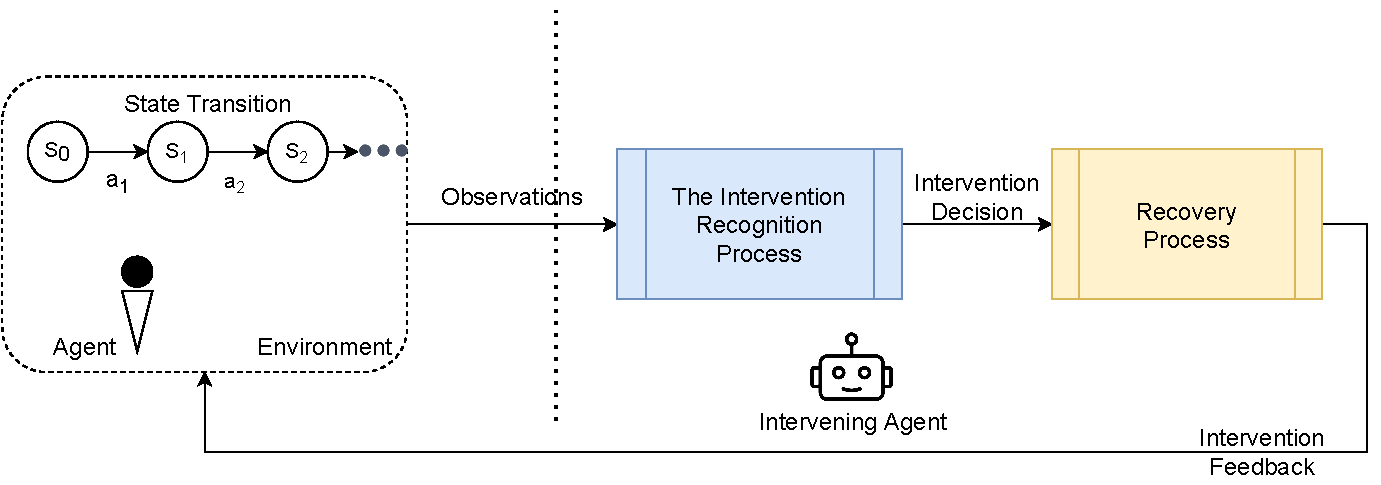
\includegraphics[width=\columnwidth]{img/interventionrecognition.pdf}}
   \caption{The stages of intervention}
\label{fig:stages}
\end{figure}

The second stage of the intervention process is \textit{\textbf{the intervention recovery process}}. 
It is natural to envision the intervention decision to manifest as an alert message for the agent in the intervention feedback loop. 
The simplest case of helping the user through intervention is to adopt a preventive measure such as blocking the recognized dangerous action or displaying an alert.
This approach makes sense in domains like cyber-security because once the attack is complete, reverting back to a safe state may be difficult. 
Furthermore, the user may not even be aware that an attack has taken place until long after. 
Examples of intervention actions include: cleaning attachments of a particular type, updating a software version or installing a firewall. 
In other domains, the preventive measures may not be as helpful. 
For example, if the intervention occurs when the human user is learning to use a new software application, the observer in addition to blocking the action, must also help the user in framing the decision about what to do next.
Therefore, in the intervention recovery process, we ask the question: \textit{can we improve the intervention recovery process to guide the user toward a desirable outcome while avoiding undesirable outcomes instead of blocking actions?} 
This is an important question, specially in cases where the agent is a human user. 
To answer this question, we present an \textbf{intervention feedback technique built on automated planning} to safely guide the user toward the goal.
The intervention feedback technique helps a human user complete a cognitively engaging problem solving task by providing helpful hints. 
A hint is a piece of information about the search problem the user is solving. 
We design helpful hints to allow the user to carefully probe the solution space of the problem during the search, while avoiding the undesirable consequence.
In this dissertation, we explore how automated planning can be used in:
\begin{itemize}
\item modeling the intervention environments
\item intervention recognition process
\item intervention recovery process
\end{itemize}
Automated planning is integral to the design of the intervening agent. 
First, planning is used to model the intervention environment as a state transition system comprised of preconditions and post-conditions of actions. 
Second, to achieve some goal in the environment, the user executes many actions; while a few of them incur risk, some are pivotal in triggering the undesirable consequence. 
Therefore, in order to identify when intervention is needed the observer must be able to generate alternative plans to find the many possible ways to reach the undesirable consequence. 
Third, when intervention occurs the user may still be incapable of deciding what to do next on his own, mainly because of hidden information about the domain or the actions of an adversary that the user can not control. 
Therefore, planning can be used to implement preventive measures such as blocking. 
Once the paths leading to an undesirable consequence have been identified, the planner can be provided with intervention actions that negates the states leading to the undesirable consequence. 
The preconditions of an intervention action are  states that are on the path to the undesirable consequence and the post-conditions of the intervention action negates that specific state. 
In situations where the user needs more help than a simple preventive measure, as we will show in this dissertation, automated planning can be used to help guide the user toward a plan that avoids the undesirable consequence.
Good intervention actions are those that block multiple undesirable consequences, are low cost to execute and do not interfere with the user’s needs or preferences. 
In this dissertation, we discuss three intervention models that address two of the aforementioned requirements, blocking multiple undesirable consequences and not interfering with the user's needs. 
\begin{description}
\item [Recognition of actions that ensures safety while allowing some freedom for the user : ] The observer and the user operate in an unfamiliar and online environment, where partial knowledge about the environment precludes the user from recognizing an unsafe state. 
The observer has knowledge about the user's desirable goal and the unsafe state the user likes to avoid.
We discuss the design of an observer that can intervene and guide a user toward a desirable outcome while avoiding undesirable outcomes or frustration.
When recognizing where intervention is required, the observer considers both the user's goal and the undesirable state.
Furthermore, the observer needs to allow the user reach his goal and not be constantly interrupted.
We present two intervention models that combine automated planning and machine learning. 
The observer can adopt these models to help the user reach the desirable goal while avoiding the undesirable state.
\item [Recognition of actions that enable multiple undesirable consequences : ] Using a cyber-security application, we study intervention when the observer is not aware of the user's goal, but still needs to help the user avoid multiple undesirable states in the environment. 
Because the user's goal is unknown, the observer cannot determine when to intervene based on the user's goal and the undesirable state. Therefore, we frame the observer's decision to recognize when intervention is required as a function of objective metrics. The objective metrics capture the timeliness and criticality of actions that must be flagged for intervention in order to help the observer identify at an opportune time, the actions that may cause the most damage. 
We also investigate how the missing and extraneous actions in the observation trace affects the intervention decision.
\end{description}
In both recognition types, the observer must deal with a trade-off in early recognition of potential danger versus certainty that the undesirable effects will occur. 
In this dissertation, we investigate different metrics to capture that trade-off and how to combine different objective metrics to identify pivotal actions.

\section{The Dimensions of an Intervention Problem}
Let us now look at an example application that requires intervention.
Figure \ref{fig:episode} models an application in the Blocks World domain \cite{gupta1992bw}, where two agents: a user and a competitor stack blocks to spell the words BAND and BRAND respectively.
In the environment, the user and the competitor perform the actions \textsc{pick-up}, \textsc{unstack}, \textsc{stack}, and \textsc{put-down} using the blocks A, B, N, D and R. 
The user can not recognize the block R.
The competitor uses the hidden block R to subvert the user's goal BAND and achieve his goal BRAND.
We refer to the user's goal BAND as the desirable goal (\desired) and the competitor's goal BRAND as the undesirable state (\undesired).
When the competitor and the user present actions to the observer, the observer must help the user achieve BAND while avoiding BRAND. 
The observer does this by accepting actions that help the user advance toward the goal BAND and rejecting the actions that do not. 
In this example, when the user first presents the action \textsc{unstack a b}, the observer asks the question: ``\textit{will the user avoid the undesirable state if the presented action \textsc{unstack a b} is accepted as an observation}?''
If the observer's analysis finds that the user will not avoid the undesirable state, then intervention occurs and the process moves on to the intervention recovery phase.
In the intervention recovery phase, the observer accepts actions that help the user advance toward \desired and rejects actions that enables or satisfies the undesirable state.
The actors continue to present actions until the user achieves \desired.
The observer makes the intervention decisions in favor of the user for each presented action.
\begin{figure}[ptb]
  \centering
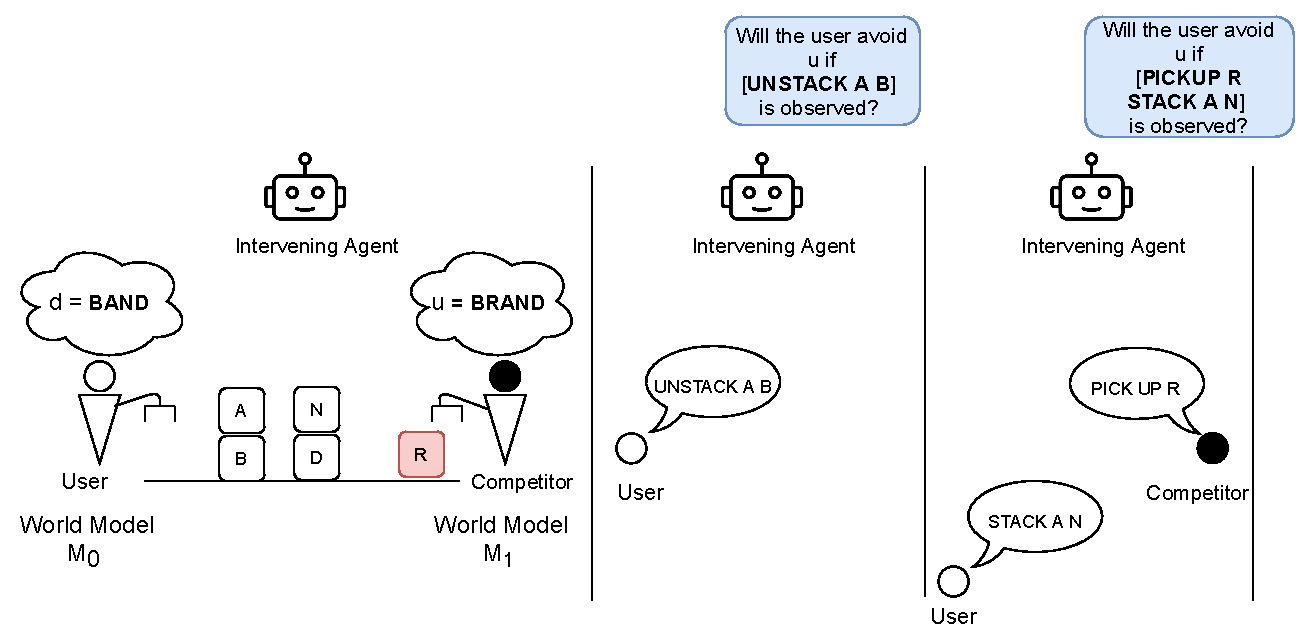
\includegraphics[width=\columnwidth]{img/episode.pdf}
\caption{An intervention episode modeled in the Blocks Words domain}
\label{fig:episode}
\end{figure}

We study several properties in the intervention environment in order to discuss the dimensions of an Intervention Problem, taking a cyber-security application and a cognitively engaging puzzle solving task as examples.
\begin{description}
\item [Actors in the environment :] The observer may be monitoring the user working alone or the user working with other agents in the domain. 
The example in Figure~\ref{fig:episode} shows a scenario where the observer monitors two actors. 
The intervention models we discuss in this dissertation consider both single agent and multi-agent intervention.
When there are other agents working to achieve goals that are different to the user's, the observer must  analyze how the post conditions of the other agents' actions affect the user's goal achievement. 
We can not assume that only the other agent's actions will always result in the undesirable state.
Sometimes, the other agents may execute actions that enable the undesirable state, but the undesirable state does not actually manifest until much later, possibly when the user executes an action that appear to be harmless. 
For example, consider a phishing attack. 
The attacker enables the attack vector by sending the phishing email to steal the user's password. However, the user's password does not get stolen until the user clicks on the link (normally, a  harmless action) to visit the phishing site and submits the information.
Recognizing these enabling actions allows the observer to intervene the user in advance and give the user some time to recover.
\item [Goals hidden to the observer :] To help the user trade-off benefits versus risks, the observer needs to know what the user thinks he/she is trying to accomplish.  
Using automated planning, we can categorize goals of the user and other actors in the environment in terms of  actions and their post conditions. 
However, in certain cases, specifying the user's goal may be difficult. 
For example, consider a home computer user preparing a document to send as an attachment in an email, while listening to music. 
In this situation, the home computer user will not be able to explicitly state his goals as post conditions of actions to the observer as required by planning.
At different times, the human user may change the order in which he wants to achieve the goals. 
For example, at the start he may want to play music in the background (as a secondary goal) while preparing the document (primary goal).
However, if he hears a song he doesn't like he may want to pause the document preparation task and change the song on the music player.
In this situation, the user's priorities change.
Therefore, in certain cases, the observer must also be able to make the intervention decision considering only the undesirable states the user wants to avoid.
\item [Types of observations :] In the example shown in Figure~\ref{fig:stages}, the observer makes the intervention decision based on actions presented by the actors. 
We make the differentiation between observations of actions and observations of state because in some intervention scenarios, the observer may not be able to observe the action itself but will be able to perceive the post conditions of the action in the environment. 
For example, consider the situation where a remote attacker sends a phishing email to the user. The observer may not be able to observe the action of sending the email.
However, the post condition of that remote action, i.e., the presence of the phishing email in the user's inbox, can be perceived by the observer.
When the actions are unobservable, the states resulting from actions can be used to extract the information necessary for the intervention decision.
Our intervention models consider both the observations of actions and states to decide when to intervene.
\item [Noise in observations :] When an agent or a human user executes actions to achieve a goal, lots of extraneous actions can be thrown into the observation trace. 
This is because the user does not intentionally want to trigger the undesirable state. Rather, he is trying accomplish a different (and useful) goal in the domain. 
This means that the plans that lead to the undesirable states may not encompass the user's goal and as a result, the observations will contain not only the undesirable actions, but also the desirable actions.
In addition to extraneous actions, the observer may miss some actions executed by the actors because of faulty sensors. 
Using the cyber-security domain as case study, we explore the impact of noise in the observation trace in making a correct intervention decision.
\item [Intervention recovery :] In this work, we model the observer as an agent who can intervene to help the user reach the desirable goal safely. We present two intervention models with different intervention recovery processes.
In one form of intervention, the observer considers the remaining plans in safe and unsafe partitions to learn to recognize unsafe suffixes in order to help the user avoid the undesirable state.
In this case, the observer can help the user by only accepting actions into the observation history that will safely advance the user toward the user's desirable goal.
In the second form of intervention, the observer learns to recognize that the user is not making progress toward \desired by analyzing the observation history when a suffix is not available. In this case,  the observer must offer enough help to \textit{guide} the user toward \desired without giving the solution. 
The second intervention model is particularly useful when the user is a human and it can be difficult evaluate progress with heuristics like a normal planning agent.
\end{description}


\section{Intervention Use Cases}
Users perform many actions in order to complete a task; while a few of them incur much risk, some are pivotal in triggering vulnerabilities. 
Given there are necessary preconditions in the system, either created by the user or by an adversary, any seemingly harmless action can suddenly become dangerous. 
The Intervention models allow us to automatically detect such vulnerable situations.
We discuss helpful intervention using two use cases. 
The uses cases we selected to study intervention have different dimensions. 
Table \ref{tab:properties} summarizes the intervention dimensions for each domain.
\begin{table}[tpb]
\caption{Dimensions of intervention use cases}
\label{tab:properties}
\resizebox{\columnwidth}{!}{%
  \begin{tabular}{|l|l|l|}
\hline
& \multicolumn{2}{c|}{\textbf{Domain}}  \\ \cline{2-3} 
\multicolumn{1}{|c|}{\textbf{Dimension}} &
  \multicolumn{1}{c|}{Cyber-security} &
  \multicolumn{1}{c|}{Rush Hour} \\ \hline
Actors in the environment  & User, Attacker, Observer & User, Observer \\ \hline
Goals hidden to the observer &
  \begin{tabular}[c]{@{}l@{}}User's goal is hidden\\ 
  Multiple known undesirable states \end{tabular} &
   \begin{tabular}[c]{@{}l@{}}User's goal is not hidden\\ 
  One or more known undesirable states \end{tabular} \\ \hline
Types of observations &
  \begin{tabular}[c]{@{}l@{}}The observer observes user's actions\\ 
  The observer only observes the effects of the attacker's actions\end{tabular} &
  The observer observes user's actions \\ \hline
Noise in observations     & Has missing and extraneous observations & None                           \\ \hline
Intervention recovery  & block action & Offer helpful hint   \\ \hline
\end{tabular}%
}
\end{table}

\subsection{Intervention in Cyber-security}
In the cyber-security domain, we model an attacker attempting to trick the user into compromising his security/privacy during day-to-day computing tasks.
The attacker creates opportunities for phishing and malware attacks by making them to appear as common harmless tasks such as email and installing software.
Unable to recognize these attacks in advance, the user becomes an unwitting accomplice to security breaches. 
The Intervention Problem for the cyber-security domain consists of three actors: the human user, the attacker (human/machine) and the observer. 
In most cyber-security cases, the attacker does not operate as a typical adversary (e.g., taking turns with the user). 
Instead the attacker takes preemptive actions and lays traps (e.g., send phishing email), which are often tied to typical actions the user performs (e.g., checking email). 
We model the cyber-security domain with multiple undesirable states: phishing attacks, malware installations. However, the user's goal is hidden to the observer.
In the cyber-security domain we model noisy observations in terms of missing and extraneous actions.
The observer considers the actions of the user and the post-conditions of attacker's actions to produce the intervention decision. 
The observation trace will contain varying noise levels from missing and extraneous actions.
Our helpful intervention solution for cyber-security is based on automated planning and uses the properties of a planning problem to identify ``\textit{critical trigger actions}'', that will cause the security breach. 
We do not study a specific recovery process for Cyber-security domain. 
We assume that when the observer identifies the critical trigger action, it is blocked.

\subsection{Intervention in Rush Hour}
Our second case study is a puzzle solving task called Rush Hour, which simulates a parking lot. In the standard version of the puzzle, the player has to clear a path on a board to move a target vehicle to the exit. To simulate the condition where the user is working only with partial knowledge about the domain, we introduced a hidden forbidden vehicle to the Rush Hour puzzle, which if moved will cause the undesirable state. 
We use the Rush Hour puzzle to approximate the case where human users learn to use a new software application and also it helps motivate the users to actually do the task in experiment conditions. 
The Rush Hour domain only has the human user and the observer. 
Unlike the cyber-security use case, the observer is aware of the desirable goal the user is trying to achieve (i.e., solve the puzzle by moving the target vehicle to the exit) and also the undesirable state (i.e., forbidden vehicle moves).
Similar to the cyber-security use case, the Rush Hour domain also contains multiple undesirable states. All states resulting from legal moves of the forbidden vehicle are undesirable.
The observations are actions the user executes to solve the puzzle. In this case, the observations are not noisy.
Our intervention solution for this case uses machine learning algorithms to recognize when the user is about to move the forbidden vehicle and intervene.
As the recovery process, we explore how to help the human user decide what to do next by offering further assistance as helpful hints.
In both cases the user actively pursues his own goal. 
The threats are triggered because the user did not understand the consequences of reaching the undesirable state (phishing/malware vulnerabilities) or was not aware of the undesirable state from the start (hidden forbidden vehicle in Rush Hour). 
The observer makes the decision to intervene upon recognizing actions in the observations that enable or satisfy the undesirable state.
 
\section{Distinguishing Intervention From Plan Recognition}
Plan recognition is the closest to our Intervention Problem. 
In the literature the plan recognition is defined as the problem of taking as input a sequence of actions performed by an actor and inferring the goal pursued by the actor and also organizing the sequence as a plan structure \cite{kautz1986generalized,schmidt1978}. 
The solution to the plan recognition problem is given by the set of goals that produces a plan that is compatible with the observations. 
The online version of the plan recognition problem uses observations as they happen as input. 
The offline version requires the complete observation to be available in advance. 
At first glance, it might seem that intervention is a variant of Plan Recognition for the user's desirable goal and the undesirable states the user wants to avoid. 
However, there are several subtleties that make intervention unique, which we now discuss.
\begin{itemize}
\item \textbf{Intervention is an online problem.}
In most cases Plan Recognition (e.g., \cite{ramirez2009plan,ramirez2010probabilistic, sohrabi2016plan}) is an offline problem;
there are a few notable exceptions \cite{mirsky2018}.
However, intervention is inherently online and dynamic.  
The observer decides whether to intervene (or not) every time the user(s) presents an action.
In order to make the decision, the observer uses the observation history, which contains accepted actions.
Intervention is a multi-agent problem as well. 
This has ramifications in environments where the user and the competitor compete to achieve close but different goals. 
With intervention, the observer can help the user by accepting actions into the observation history that only help further the user's goal. 
This is not possible with offline plan recognition.
\item \textbf{Agents may have distinct views of the problem.}  
The user and the competitor are modeled with different domain definitions. 
When the agents have distinct views of the problem and they can not satisfy the undesirable state on their own, conditions will arise such that the agents working together will enable the undesirable state.
The user wants to satisfy the desirable goal state, while avoiding the \textit{hidden} undesirable state.
The competitor is trying to subvert the user’s goal by enabling preconditions for the undesirable state without the user's knowledge.
When the user and the competitor reveal their plan(s) incrementally, the observer needs to decide whether the revealed actions make it impossible for the user to avoid the undesirable state considering the plans from the user's and the competitor's domain definitions collectively. 
Any action that make it impossible for the user to avoid the undesirable state must be flagged for intervention and not accepted into the observation history.
If the plans for the undesirable state and desirable goal share a long common prefix, 
it will be difficult for the observer to disambiguate between the goals and to use plan recognition algorithms in time to help the user avoid the undesirable state.
\item \textbf{Partitioned suffixes (with known desirable goal).}
When the desirable goal is known, the observer should allow the user to pursue suffixes leading to the desirable goal and intervene when actions are presented from suffixes that get ``too close'' to the undesirable state. 
Our key insight is to model the  ``goals'' of the user and competitor, which justifies our use of planning to find these suffixes. 
However, intervention adds new concerns beyond plan recognition, namely that the observer needs to consider two kinds of goals that might require intervention:
\begin{enumerate}
\item Cases where the user is headed toward a undesirable outcome. 
This can be easily be solved by plan recognition.
\item Cases where the user unwittingly enables an undesirable outcome by taking actions toward a desired goal. 
This is less easily solved by plan recognition because there is an inherent trade-off between intervening and allowing the user some freedom to pursue the desirable goal. 
Suppose that some suffix $\Suffix_{\undesired}$ leads to the undesirable state and suffix $\Suffix_{\desired}$ leads to the desirable goal.  
Then it can happen that by simply following the plan leading to the desirable goal, the user enables the undesirable state when there is enough overlap between  $\Suffix_{\undesired}$ and $\Suffix_{\desired}$.
\end{enumerate}
Partitioning the suffixes this way allows the observer to learn the differences between the safe and the unsafe suffixes and balance specific unsafe actions with those that are necessary for allowing the user some freedom.
For example, in a malicious email attack such as phishing, the user will still want to check email.
So prohibiting email is untenable; what the agent must do is intervene when the user attempts to click the phishing link.
This need for partitioning the suffixes  is distinct from plan recognition, where existing offline Plan Recognition algorithms often rely on  plan cost to disambiguate between goals and recognize suffixes. 
When the undesirable state and the desirable goal are too close, disambiguation based on plan cost will not work (we will demonstrate in a later chapter). 
Learning the differences between the plan partitions will allow us to address this issue.
\item \textbf{Suffix analysis with unknown desirable goal.}
When the desirable goal is unknown, the observer only has the space of plans leading to the undesirable goals to make the intervention decision when the agents reveal their plans incrementally.
Plan recognition over the undesirable goals does not really     apply because it is     focused on matching actions to  prior plans     to determine the goals the      user is trying  to achieve.     
In other words, the observer assumes that the user is executing some plan to reach the undesirable state.
In reality, the user wants to avoid the undesirable state and reach a different (desirable) goal, which may be unknown to the observer.
Therefore, when analyzing partition suffixes with known desirable goal, the observer uses the knowledge of the user's goal to determine which are critical actions that require intervention.   
In contrast, with unknown desirable goal, the observer analyzes the remaining undesirable suffixes to identify actions that cause the most damage to intervene the user.
\item \textbf{Goal priors cannot be estimated reliably.}  
Plan Recognition algorithms use a prior probability distribution over the goal hypotheses to estimate the posterior probability of the likely goals given the observations. 
Intervention must consider the likely goals regardless of their priors. 
For example, the undesirable state is hidden from the user, who does not intend to achieve it (i.e., prior probability $\approx 0$). 
In contrast, a competitor, when present, intends to achieve the undesirable state (i.e., prior probability $\approx 1$).
When the priors are not accurate, the observer (using Plan Recognition) may not be able to  disambiguate between likely goals (and recognize the correct plan) in time to avoid the undesirable state.
  
\item \textbf{Emphasis on intervention recovery.}
In Plan Recognition, the observer uses an observation trace to derive the user's likely plan. 
The observation trace can be either an ordered sequence of actions  \cite{ramirez2009plan,ramirez2010probabilistic} or an ordered sequence of states \cite{sohrabi2016plan}.
Plan Recognition does not define a method for the user to recover when the observer recognizes a plan leading to the undesirable state. 
With the proposed intervention models, we address that limitation with two different types of help the observer can offer to the user to decide what to do next.
\end{itemize}


\section{Research Questions}
The main objective of this research is to study different intervention models that help human users complete tasks safely. We address the following research questions: 
\begin{description}
\item[What are the salient characteristics for deciding when to intervene?]
We address this question considering the dimensions of an intervention problem, summarized in Table~\ref{tab:properties}.

Our intervention models are based on identifying actions in an observation trace that either satisfy the undesirable state or enable it. 
This requires the observer to evaluate the current state (i.e., state resulting from the observed actions) based on it's importance to causing the undesirable state considering the user's desirable goal (if available) and the undesirable state.
In the two intervention use cases, criticality of the current state is evaluated using two different methods. 
For the cyber-security domain we identify salient features by analyzing the plan space. 
We model the cyber-security domain as a planning problem and use an existing automated planner to  sample the possible solutions (plans) that project possible undesirable outcomes and then trace back to actions critical to their occurrence. 
The resulting plans are analyzed to extract objective metrics to predict if the current action is likely to trigger the undesirable consequences. 
Raising a warning to the user involves a trade-off in early recognition of potential danger versus certainty that the effects will occur. 
We investigate different objective metrics to capture that trade-off and how to combine these objective metrics to identify pivotal actions. 

To study intervention in the Rush Hour domain, we formalize a family of Intervention Problems and show how these problems can be solved using a combination of Plan Recognition methods and classification techniques to decide whether to intervene. 
We characterize the observer's decision space as an Intervention Graph and construct it using an ``Intervention as Classical Planning'' approach to generate potential suffixes of partially executed plans. 
We extract domain-independent features from this graph and extend several Plan Recognition benchmarks to evaluate this approach. 
We then generalize these results to Human-Aware Intervention, where the observer must decide in
real time whether to intervene for human users solving a cognitively engaging puzzle. 
Using a revised feature set more appropriate to human behavior, we produce a learned model to recognize when a human user is about to trigger an undesirable outcome.

\item[How should information be displayed to effectively inform users following intervention?] Using the Rush Hour domain, we study how an intervention model can be extended to help users continue a cognitively engaging task by providing helpful hints. 
In the context of the Rush Hour puzzle solving task, a hint is a piece of information about the Rush Hour search problem. 
We design helpful hints to allow the user to carefully probe the search space of the Rush Hour search problem, while avoiding the undesirable state.
We monitor how human users achieve planning landmarks of the Rush Hour problem when intervention is supported by hints compared to intervention without hints to evaluate the effectiveness of our intervention recovery process.

\item[How to design tools to study intervention in activities with human user participation?]
To identify pivotal events, the appropriate system states and user actions must be monitored and compared to a model of actions that can lead to the undesirable state. 
If an action that contributes to a trigger is suspected, it should be put in the context of what the user is trying to do and an estimate of how likely the action is to actually cause the undesirable state. 
We develop state/action models using automated planning that allow us to recognize the appropriate system \textit{states} (computer/puzzle board) that must be monitored and the \textit{actions}, which may lead to the undesirable state. 
For the cyber-security domain, we model the security vulnerabilities that occur in a home computer environment using PDDL (Planning Domain Definition Language) \cite{ghallab1998}, which is designed to represent pre-conditions and post-conditions of actions. 
PDDL is the prominent representation used in the AI Planning community. 
We also develop PDDL models for the Rush Hour domain, which will be used in generating the helpful hints. 
Our studies are focused on how human users solve these tasks (e.g., perform common home computer user actions, solve a Rush Hour puzzle), which requires studying human users in situ. 
To this end, we will develop a simulated home computer environment for studying users practice computer security and a Rush Hour puzzle simulator to study how human users respond to helpful hints. 
Both these tools are event monitoring systems that capture human user's actions when placed in different experimental conditions as well as system level events that are defined in the PDDL models.
\end{description}


The rest of this dissertation is organized as follows:
\begin{itemize}
\item \textbf{Chapter 2}: We present the background on automated planning and a review of existing plan recognition literature that studied methods to infer an agent's intention.
\item \textbf{Chapter 3}: We present the findings of an human subject study to motivate plan intervention. In this study, we simulate cyber-security vulnerabilities that occur in a home computer environment when the human users perform routine tasks like checking email and using software applications.
\item \textbf{Chapter 4}: We present the first intervention model based on the findings of the cyber-security human subject study. 
We formulate the Intervention Problem as a  planning problem of three domain independent objective metrics: timeliness, which captures how soon the undesirable state may occur; certainty, which captures how frequently the undesirable state may be seen; and desirability, which captures the user’s preference for continuing the current action despite the increased risk. 
Against an ideal baseline, we examine trade-offs in choosing the ``correct'' intervention point by varying the weights associated with these objective metrics, the observability of actions, and the presence of extraneous actions.
\item \textbf{Chapter 5}: We study two kinds of Intervention Problems in environments where an observer monitors a user (and a competitor) and help the user achieve a desirable goal, while avoiding an undesirable state. 
In ``\textbf{Unsafe Suffix Intervention}'', the observer uses automated planners to project the remaining suffixes and extract features that can differentiate between safe and unsafe plans. 
We evaluate the recognition accuracy of Unsafe Suffix Intervention on benchmark planning
problems. 
In ``\textbf{Human-aware Intervention}'', the observer uses the observed partial solution to extract features that can separate safe and unsafe solutions. 
We evaluate the accuracy of Human-aware Intervention on a new Intervention Planning benchmark Rush Hour.
\item \textbf{Chapter 6}: We present an intervention recovery process for the Human-aware Intervention model based on automated planning. 
We discuss the findings of a human subject study where human users solved a cognitively engaging Rush Hour puzzle task while being guided by a human-aware intervention agent. 
We evaluate the efficacy of our recovery approach using automated planning landmarks.
\item \textbf{Chapter 7}: We discuss some open issues in Intervention and provide an outline for future research.
\end{itemize}


\chapter{Preliminaries}
\label{chap:ch2}
In order to design intervention for human users, first we need to model human user behavior in some environment. 
We use the automated planning formalism \cite{nau2004} to describe the tasks the user performs in both the cyber-security and Rush Hour domains. 
The automated planning formalism is based on concepts such as goals, states and actions, to describe the behavior of rational agents. 
Although human user behavior is more complex than that of a rational agent, in our intervention models we assume the actor being intervened is a (bounded) rational agent.
In this chapter, we first present an overview of automated planning and describe how a state/action model can be represented as a classical planning problem. Next, we discuss the problem of inferring the intention of an agent and discuss three variants of the problem: plan recognition, goal recognition and activity recognition. Finally, we present a discussion on the existing literature on intention recognition considering a three-dimensional framework: number of agents in the environment, online/offline recognition and how the recognizer interacts with the environment during the intention recognition process.

\section{Automated Planning}
Planning aims at achieving some predefined objectives through a deliberation process that chooses and organizes actions by anticipating their outcomes. The planning formalism views the problem as a state transition system, defined as a tuple $\Sigma=(S,A,E,\gamma)$ where:
\begin{itemize}
\item $S = \lbrace s_1, s_2, \ldots \rbrace$ is a finite or recursively enumerable set of states;
\item $A = \lbrace a_1, a_2, \ldots \rbrace$ is a finite or recursively enumerable set of actions;
\item $E = \lbrace e_1, e_2, \ldots \rbrace$ is a finite or recursively enumerable set of events; and
\item $\gamma: S\times(A\cup E)\mapsto 2^S$ is a state transition function.
\end{itemize}
Given an action $a\in A$ and $\gamma(s,a)\neq\emptyset$, then $a$ is \textit{applicable} in state $s$. If $a$ is applied to the state $s$, it will take the system to a different state $s^\prime\in \gamma(s,a)$. A state transition system $\Sigma$ can be represented in a directed graph $G=(V_G,E_G)$, where $V_G=S$ and an edge $e_G\in E_G$ connects two states $e_G=s\mapsto s^\prime$, labeled with an action $a$ if and only if $s^\prime \in \gamma(s,a)$ as shown in Figure~\ref{fig:blockswords}. 

In this example, we model the Blocks Words problem \cite{ramirez2009plan}, which is a modification of the Blocks World domain \cite{gupta1992bw}. In the Blocks Words problem, the agent operates in an environment that contains a flat surface (a table) and a set of blocks identified by English letters. The blocks can be stacked on one another. The agent uses a set of actions (e.g., pick-up, put-down, stack, unstack) to build a stack such that it spells a word from the top to bottom (i.e., goal state). The agent can only move one block at a time. The agent's goal is to spell the word BAND. Initially, the blocks D, N are on the table and B is stacked on A. The partial graph shows some of the the state transitions that can happen in the domain. Red color edges show a path (i.e., an action sequence), which translates the initial state to the goal state. Let us map the Blocks Words environment in Figure \ref{fig:blockswords} to the definition of $\Sigma$.
\begin{itemize}
\item $S = \lbrace init, goal, s_1, s_2 \ldots \rbrace$ is a finite or recursively enumerable set of states;
\item $A = \lbrace pickup, unstack, stack, putdown \rbrace$ is a finite or recursively enumerable set of actions;
\item $E = \lbrace \rbrace$ assuming no exogenous events occur and;
\item $\gamma:$ transitions indicated by arrows in the graph.
\end{itemize} 


The state transition system $\Sigma$ describes all the ways in which our environment may evolve. Finding a \textit{plan} means that we need to extract a structure that gives appropriate actions to apply such that some \textit{objective} can be achieved. There can be many forms to define this objective: (1) defining a goal state or a set of goal states (e.g., state \textit{Goal} in Figure~\ref{fig:blockswords}), (2) optimize for a utility function attached to the states, (3) satisfying some condition over the sequence of states, (4) defining tasks to be performed. In our work, when we refer to the \textit{objective}, we mean type (1) objective.

The preliminary intervention designs are for an agent whose behavior can be represented using a classical planning model. The classical planning formalism requires eight restrictive assumptions about $\Sigma$:
\begin{enumerate}
\item The system is defined using a \textbf{finite} sets of states, actions and events.
\item The system defined in $\Sigma$ is \textbf{fully observable}. This means that the agent has knowledge  about every aspect of the state when an observation is made.
\item The system defined in $\Sigma$ is \textbf{deterministic}, i.e., an action in the system does not have alternative outcomes. Formally, for all $s\in S, u\in A\cup E; |\gamma(s,u)|\leq1$
\item The system define in $\Sigma$ is \textbf{static}, i.e., there are no exogenous events happening in the environment. $E=\emptyset$
\item Only \textbf{restricted goals} can be given to the planner. Restricted goals are given as an explicit goal state or a set of goal states.
\item The solution plan for a planning problem in $\Sigma$ is a linearly ordered finite sequence of actions.
\item The system defined in $\Sigma$ has \textbf{implicit time}. This means that actions and events do not have any time duration between state transitions.
\item Planning in $\Sigma$ is \textbf{offline}, which means that any changes to $\Sigma$ that takes place while the planner is searching for a plan, are ignored.
\end{enumerate}

Given a description of $\Sigma$, the initial state and an objective, an automated planner generates a plan that achieves the objective. A classical plan for the Blocks Words problem is a sequence of actions (e.g., \texttt{unstack B A, put down B, pick up N}, etc.). A plan can also be represented as a policy: a partial function from $S$ into $A$ (e.g.,  $\lbrace$(\texttt{init, unstack B}), ($s_1$,\texttt{ putdown B}), ($s_4$,\texttt{ pickup N}) $\ldots\rbrace$. When we refer to plans in this work, we mean a sequence of actions. The agent can execute these plans on the environment using actuators, which generates observations. In our Blocks Words example, the agent can use a mechanical arm to lift block B from the top of A. This generates an observation, the mechanical arm holding block B and the top of block A now being clear. Formally, the agent's behavior can be defined as a \textbf{planning problem} $P=(\Sigma, s_0, S_g)$ where, 
\begin{itemize}
\item $\Sigma=(S,A,\gamma)$ is a state transition system,
\item $s_0\in S$ is the initial state and
\item $S_g\subset S$ is a set of goal states.
\end{itemize}
\noindent The solution to $P$ is a sequence of actions $\langle a_1, a_2, a_3, \ldots, a_n\rangle$ such that it corresponds to a sequence of states $\langle s_0, s_1, s_2, \ldots, s_n\rangle$ where $s_1=\gamma(s_0,a_1), s_2=\gamma(s_1,a_2), \ldots, s_n=\gamma(s_{n-1},a_n)$ and $s_n \in S_g$

\begin{figure}[ht]
  \centering
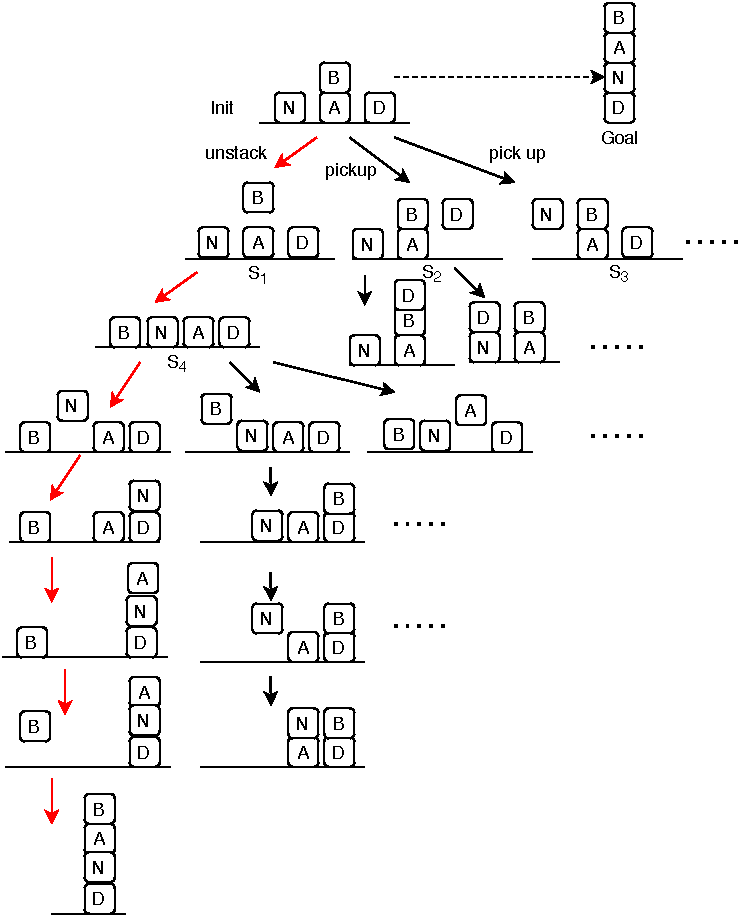
\includegraphics[width=0.6\columnwidth]{img/bw.pdf}
  \caption{Blocks Words problem as a state transition system}
  \label{fig:blockswords}
\end{figure} 

\section{Representing Classical Planning Tasks}
Although we can use the graph representation of the state transition system corresponding to a planning problem, the resulting graph can be very large and modifying this graph as new events occur in the system can become very cumbersome. In order to provide a compact representation of the transition system, \textit{states} (i.e., vertices) are represented using state variables, and actions (i.e., edges) are represented as \textit{operators} with preconditions and post-conditions specified as state variables. This way, in order to find a plan, we only need to provide the initial and goal states and use the operators to find other states as needed.

A classical planning problem can be represented using the \textbf{classical representation}, \textbf{the set-theoretic representation} or \textbf{the state-variable representation}. STRIPS \cite{fikes1971strips}, which we will use to model the domains described in this work, is an implementation of the classical representation. STRIPS uses first-order literals to describe states and actions. The set-theoretic representation is used when planning problems are solved with SAT solvers. The state-variable representation is implemented in SAS formalism \cite{backstrom91}.

In the classical representation, the world state is a set of \textbf{grounded} propositional state variables. $\Sigma$ is described using a finite set of grounded propositional state variables, which means there are only finitely many possible states. Operators that modify the world state consist of precondition propositions: propositions that must be true for the action to execute, and post-condition propositions: those will be made true as a result of the action. An \textit{action} is a ground instance of an operator. The initial state in the Blocks Words example in Figure~\ref{fig:blockswords} described in the grounded classical representation is: $\lbrace$
\texttt{ontable(N)}, \texttt{ontable(A)}, \texttt{ontable(D)}, \texttt{on(B,A)}, \texttt{clear(N)}, \texttt{clear(B)}, \texttt{clear(D)}$\rbrace$. The operator unstack is described as: \\
\textbf{operator}: \texttt{unstack (x, y)}\\[-0.5em]
\textbf{preconditions}: \texttt{(on x, y)},\texttt{(clear x)},\texttt{(handempty)},$\neg$\texttt{(equals x y)}\\[-0.5em]
\textbf{effects}: \texttt{(holding x)},\texttt{(clear y)},$\neg$\texttt{(clear x)},$\neg$\texttt{(handempty)},$\neg$\texttt{(on x, y)}

\noindent Grounding the unstack operator using blocks B and A defines the action as follows:\\
\textbf{action}: \texttt{unstack (B, A)}\\[-0.5em]
\textbf{preconditions}: \texttt{(on B, A)},\texttt{(clear B)},\texttt{(handempty)},$\neg$\texttt{(equals B A)}\\[-0.5em]
\textbf{effects}: \texttt{(holding B)},\texttt{(clear A)},$\neg$\texttt{(clear B)},$\neg$\texttt{(handempty)},$\neg$\texttt{(on B, A)}

\noindent An action is \textit{applicable} in state $s$ if $s$ satisfies the preconditions of the action. 
This means that the action's positive preconditions are  in $s$ whereas the negative preconditions are not in $s$. 
In the Blocks World example, (\texttt{unstack B A}), (\texttt{pickup D}), and (\texttt{pickup N}) are applicable in the initial state. If an action is applicable to $s$, the result of performing the action means to delete the negative propositions from the state $s$ and add the positive ones. For example, if \texttt{unstack B A} is executed in the initial state, the resulting state would be $\lbrace$ \texttt{ontable(N)}, \texttt{ontable(A)}, \texttt{ontable(D)}, $\neg$\texttt{on(B,A)}, \texttt{clear(N)}, $\neg$\texttt{clear(B)}, \texttt{clear(D)}, $\neg$(\texttt{handempty}), \texttt{clear (A)}, \texttt{holding (B)}$\rbrace$. Typically, in the classical representation, the state only explicitly contains the true propositional variables. Any propositional variable that are not included in the state is considered false.


\subsection{STRIPS Planning Task}
We now present a formal definition of a STRIPS domain and planning problem. In STRIPS, a planning task is defined using a planning domain and a planning problem.
\begin{definition}
A STRIPS planning domain is a tuple $\mathcal{D}=\langle F, Op\rangle$, where $F$ is a finite set of  state variables (predicates) and $Op$ is the set of operator schema. An operator schema $op \in Op$ is a tuple $ op = \langle Pre(op), Add(op), Del(op)\rangle$ that consists of preconditions, add and delete effects respectively, where $Pre(op)$, $Add(op)$, $Del(op)$ are all subsets of $F$. Predicates and operator schema have parameter lists and can be instantiated with objects (defined later). An instantiated operator (action) $op$ is applicable in a state $s$ if predicates in $Pre(op)$ are \textit{True} in $s$. A state transition induced by an action $op$ in a state $s$ is defined as a function $\delta$:
\begin{equation*}
\delta (s,op) = \left\{\begin{matrix}
s\setminus Del(op) \cup Add(op) & Pre(op) \subseteq s\\ 
undefined & otherwise
\end{matrix}\right.
\end{equation*}
\end{definition}

\begin{definition}
A STRIPS planning problem is a tuple $P = \langle \mathcal{O}, s_0, G\rangle$, where $\mathcal{O}$ is the set of objects. Objects can be either constant or non-constant and may have a type. Constant objects are common to all instances of the domain definition and shared by planning problems defined on that specific planning domain. Non-constant objects are unique to a specific planning problem. $s_0 \subseteq F$ is the set of propositions that are true in the initial state, $G\subseteq F$ represents the goal specification.
\end{definition}

Given a domain $\mathcal{D}$ and a planning problem $P$, an automated planner generates the planning task $\Pi=\langle \mathcal{F}, \mathcal{A}, s_0, G\rangle$, where $\mathcal{F}$ is a finite set of grounded propositions, $\mathcal{A}$ is the finite set of grounded actions instantiated from the operator schemata $Op$, $s_0$ is the grounded propositions specifying the initial state and $G$ is the grounded goal specification. Objects in $\mathcal{O}$ are used to ground $\mathcal{F}$, $\mathcal{A}$, $s_0$ and $G$. Grounding replaces the variable terms in the parameter lists of the propositions, action schema, goal specifications with constant/non-constant objects. 

\begin{definition}
A solution to $\Pi$ is a plan $\pi=\lbrace a_1, \ldots, a_k\rbrace$ of length $k$ that modifies $s_0$ into $G$ by successive execution of actions  $a_1, \ldots, a_k$ 
\end{definition}

Actions in $\pi$ may have a cost that assigns a non-negative value to the action schema defined in the STRIPS domain definition. The cost function is given as $C: Op \rightarrow \mathbb{R}^0_+$. The cost of the plan $c(\pi)$ is  $\sum(c(a_i))$. The optimal solution, the optimal plan $\pi^*$, minimizes the cost. 



\section{The Recognition Task}
Besides being able to plan, in certain cases the agent must also be able to \textit{recognize} another agent's behavior. This is specially important in the domains we are studying in this dissertation where the agent acts as an assistant to the human user.

We now extend our discussion to a multi-agent setting where, we consider at least two agents: an  acting agent $A$ and an observer agent $R$. To draw a realistic example, consider the Blocks World scenario in Figure~\ref{fig:bwpr}. Agent $A$ solves a planning task $\Pi_A=\langle \mathcal{F}_A, \mathcal{A}_A, s_{I_A}, G_A\rangle$ executes a sequence of actions $O=\lbrace$\texttt{unstack D A}, \texttt{putdown D}, \texttt{unstack R P}$\rbrace$. For simplicity let us assume that $R$ does not execute any actions, and passively observes the actions $A$ executes.

\begin{figure}[tpb]
  \centering
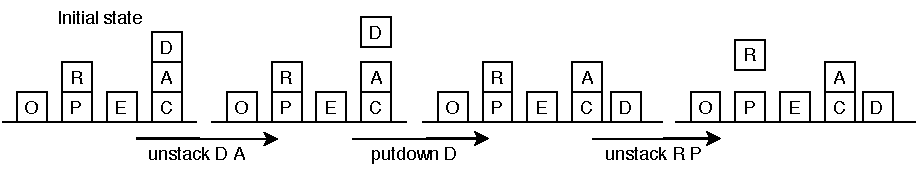
\includegraphics[width=\columnwidth]{img/bwpr.pdf}
  \caption{A recognition task}
  \label{fig:bwpr}
\end{figure}

\noindent In the recognition task, $R$ asks the question: ``What is $A$ trying to do?''. This question can be answered in three ways, leading to three types of recognition tasks:
\begin{itemize}
\item Given $O$, what is the posterior probability P($\pi$|$O$) of the complete plan $\pi$. This is the \textbf{plan recognition problem}.
\item Given $O$, what is the posterior probability P($G$|$O$) of the goal $G$, where $G \in \mathcal{G}$, a list of potential goals in the environment. This is the \textbf{goal recognition problem}
\item Given $O$, what is the posterior probability P($a$|$O$) of an activity $a$. This is the \textbf{activity recognition problem}.
\end{itemize}
\noindent Typically, $R$'s objective is to find the most likely plan, goal, activity from a set of potential plans, goals, activities in the environment. A recognition task consists of three components:
\begin{description}
\item [The environment] $E = \lbrace \Sigma, s_0, \mathcal{G}\rbrace$, is the setting in which agent $A$ acts. $s_0$ is the initial state and $\mathcal{G}$ is the set of possible goals. 
In order to perform the recognition task, the environment may produce a \textbf{plan} $\pi=\lbrace a_0, a_1, \ldots, a_n\rbrace$: a complete sequence of actions that takes agent $A$ from $s_0$ to the goal state $G$ in $\mathcal{G}$, a \textbf{history} $h=\lbrace s_0, s_1, \ldots, s_n\rbrace$: a sequence of states from $s_0$ to $G$ or an \textbf{execution} $e=\lbrace s_0, a_0, s_1, a_1, \ldots, s_n, a_n, s_{n+1}\rbrace$: a sequence of state-action transitions from $s_0$ to $G$. 
These are referred to as \textit{prefixes} in recognition. 
The recognition task example shown in Figure~\ref{fig:bwpr} considers the plan prefix. Some work in the plan recognition literature uses plan prefixes while others use the history prefixes. We will discuss work on each category. Furthermore, research has investigated recognition in both discrete and continuous domains where actions transition from one state to another via paths through the state space, rather than through discrete states (e.g., navigation domains).

\item [The acting agent (agent $A$)] must specify the assumptions made with regard to how agent $A$ acts in the environment to achieve his goal. Most of the time, recognition tasks assume that agent $A$ enters the environment and follows a plan to achieve some goal. However, $A$'s behavior may be affected by how familiar it is with the environment (e.g., are there objects that escape agent $A$'s sensors?), A's special capabilities (e.g., can he compute an optimal plan to reach $G$), and the relationship to the recognizer (e.g., does $A$ acts in such a way that his goal/plan/activity can be recognized easily or would he act to obfuscate his true goal/plan/activity?). There could be more than one agent whose goals/plans/activities we would want to recognize.
The recognition literature uses different ways to represent agent $A$ from the point of view of $R$ in the situations mentioned above. Commonly used representations are \textbf{plan libraries} and \textbf{domain theories}.

\item [The recognition system (agent $R$)] When defining a recognition problem, the final component is the specification of the recognizer. Here, we need to define several components: 
\begin{itemize}
\item the observability: how does agent $R$, perceive agent $A$'s behavior (e.g., is there any noise in the observations? Are there any actions/states $R$ can not perceive?)
\item the objective: what does $R$ need to do? (e.g., recognize $A$'s goal/plan/activity as soon as possible? is the recognition online or offline?)
\item the possible interventions: can $R$ interact with $A$ or affect its behavior? (e.g., provoke $A$ to change its course during execution, modify $\Sigma$ to help recognition)
\end{itemize}

\end{description}

We now present a framework, within which we discuss selected prior work from goal and plan recognition. We set up the framework along three dimensions:
\begin{description}
\item [single vs. multi actor] In the single actor case, $R$ makes observations of a single actor agent to recognize the goal/plan of that agent. In the multi-agent case, the observations originate from many agents. Furthermore, the goals pursued by the agents in the system may be a complex goal. For example consider an agent $X$ assisting two other agents ($Y$ and $Z$) pursuing two different goals $G_Y$, $G_Z$ respectively. $X$'s goal $G_X$ an be defined as $G_Y \cup G_Z$. Thus, in a multi-agent system $R$ may have to recognize complex goals as above, instead of one goal shared by all agents.
\item [online vs. offline] In online recognition, the observations are incrementally revealed to $R$. Recognition is performed based on the observations revealed thus far (i.e., a partial observation trace). In offline recognition, the complete observation trace is available to $R$ up front and recognition is performed accounting for information available from the full observation trace.

\item [the recognizer's interaction with the actor] In this dimension we discuss different ways $R$ can communicate with $A$ during the recognition process. In most related work, the recognition task terminates when $R$ identifies what $A$'s goal or plan is. Interaction is an extension of the typical recognition problem. Some work on interaction suggests modifying the environment (e.g., blocking some actions $A$ could otherwise have executed) to facilitate early recognition of $A$'s goals/plans. Others propose question-answering approach where $R$ queries $A$ about his plans/goals and reasoning about information acquired from the queries.
\end{description}

\noindent Within the three-dimensional framework, for each related work shown in Table~\ref{tab:relatedwork} we also discuss the properties of the \textbf{environment}, the \textbf{acting} agent and the \textbf{recognizer} agent around which the recognition tasks are modeled. Our discussion on related work also extends to work that are not listed in Table~\ref{tab:relatedwork}. We do this mainly to draw comparisons between how the work listed in Table~\ref{tab:relatedwork} improves/extends other (earlier) noteworthy plan and goal recognition work.

\begin{table}[tpb]
\caption{Fitting related work to the analysis framework}
\label{tab:relatedwork}
\resizebox{\columnwidth}{!}{
\begin{tabular}{|l|c|c|c|c|c|c|}
\hline
\multirow{2}{*}{Related Work} & \multicolumn{3}{c|}{Plan Recognition}       & \multicolumn{3}{c|}{Goal Recognition}       \\ \cline{2-7} 
                              & Single/Multi & Online/Offline & Interaction & Single/Multi & Online/Offline & Interaction \\ \hline
Ramirez et al. 2009       &        &         &      & Single & Offline & None \\
Ramirez et al. 2010       & Single & Offline & None &        &         &      \\
Sohrabi et al. 2016  	  & Single & Offline & None &        &         &      \\
Vattam et al. 2015        & Single & Offline & None & 
&  		&  \\
Vered et al. 2017 &        &         &      & Single & Online  & None \\
Boddy et al. 2005      & Single & Offline & None &        &         &      \\
Keren et al. 2014       &        &         &      & Single & Offline & Yes  \\
Pozanco et al. 2018     &        &         &      & Muti   & Online  & Yes  \\
Mirsky et al. 2016      &        &         &      & Single & Online  & Yes  \\ 
Shvo et al. 2018  	 & Multi  & Offline & None &        &         &      \\ \hline
\end{tabular}
}%
\end{table}

\section{Plan Recognition}
The plan recognition problem is to \textit{take as input a sequence of actions performed by an actor and to infer the  goal pursued by the actor and also to organize the action sequnce in terms of a plan structure} \cite{schmidt1978plan}. This requires some method to represent how the actor would act in the environment. Recognition solutions that use automated planning represent the actor's behavior as a planning problem focusing on the fact that the actor moves from state to state and changes the environment to achieve some goal. The solutions that use parsing assume that plans are constructed as a hierarchy in the actor's mind.

Early solutions to the plan recognition problem require that the part of a plan given as input to the recognizer be matched to a repository of example plans. This repository is referred to as a \textit{plan library}. The plan library represents possible plans the acting agent may be trying to execute in the environment $E$. In the plan recognition literature, several methods have been proposed as representation models of the plan library.

\subsection{Plan Recognition with Plan Library Representations}
Many plan library representations use graphs to represent a possible plan that will likely execute in the environment. 
In The Generalized Plan Recognition \cite{kautz1986generalized}, the recognition problem is defined as identifying a \textit{minimal set of top-level actions sufficient to explain the set of observed actions}. 
Here, the plans are modeled in a graph. 
The nodes of the graph represent the actions. 
The graph has two types of edges: action specialization (between top-level actions) and action decomposition into sub-actions.
The authors use a cooking domain as the example and define the top level actions and recursively decompose those actions until no further specializations can be made. 
Lower level actions in the plan graph \textit{logically imply} the higher level actions. 
For example the top level action ``PrepareMeal'' specialized into ``MakePastaDish'', specialized into ``MakeFettuciniMarinara'', decomposed into two leaf-level actions ``MakeFettucini'' and ``MakeMarinara''. The implication relationships are derived from bottom to top. Given this representation of the plan library, the plan recognition task becomes the minimum vetex cover problem of the graph. This recognition problem contains one actor and one recognizer.

Geib and Goldman represent the plan library for a cyber security domain as partially ordered AND/OR trees \cite{GeibGoldman09}. 
Their representation also assumes that the tasks the actor agent is trying to complete in the domain are hierarchical. 
AND nodes in the graph require that all sub-tasks be achieved before completing the parent task. 
OR nodes represent instances where the actor agent may choose between alternatives to complete the parent task. 
The subtasks themselves may further be represented as AND/OR (sub) trees. The root of the tree is the goal. Plans are derived from traversing to leaves from the root of the tree. The plan library is augmented with probabilities (i.e. prior probabilities of root goals, OR tree choice probabilities etc.).
Then, in order to recognize the actor's plan, the recognizer needs to compute the probability of an explanation (plan) given the observations (i.e. P$(\pi|O)$). 
Specifically, the recognizer needs to derive a probability distribution over a set of likely explanation plans. 
To extract the likely explanation plans, the authors define a grammar to parse the AND/OR trees and generatively build the explanations by starting off with a ``guess'' and refining it as more observations arrive. 
The actor in this work is hostile. This means that the actor does not want the recognizer to find out his plan and he will hide some actions. 
This causes the recognizer to deal with partial observability when computing P$(\pi|O)$. 
This topic is left for future work.

\subsubsection{Plan Libraries: What is the Problem Anyway?}
One issue with using plan libraries is that it is difficult to ensure the completeness of the plan library. It is unrealistic to encode \textit{all} possible plans for a given planning problem into a plan library. However, the system must still be able to reason about new but correct plans the agent may pursue. Cohen et al. propose a new approach for updating a plan library with new plans \cite{spencer1993}.

Another issue with using plan libraries for recognition is the noise in the input observations. A key assumption in the library based solution is that the observations must be able to associate with one or more recipes in the library, and the partial plan inferred for the agent must reflect the agent's intended goal or plan. Noise in the observation trace may occur from missing actions (e.g., noisy sensors, agent deliberately hiding observations, etc.) or exogenous events that occur in the environment that have nothing to do with the agent's true goal/plan. Rich et al. proposes  a method to enable the plan library to incrementally relax the constraints on recipes before declaring that the recipe is not found \cite{rich2001collagen}. They use a \textit{focus stack}, that maintains a set of annotated goals that are being pursued. The goals are removed from the tack only when the goal is complete.

\noindent\textbf{Vattam et al. 2015 - Case-based Plan Recognition}

The case-based plan recognition \cite{vattam2015case} relaxes the error-free requirement of the observations in plan recognition problems and introduces a recognition algorithm that can handle \textbf{missing} and \textbf{misclassified} actions in the observation trace. This problem is also modeled with a single actor and a single passive recognizer agent and assumes that there exists a plan library consisting of a set of \textit{cases}. A case consists of a planning problem and a fully grounded solution plan to this planning problem. Given a subsequence of actions, the algorithm needs to address two requirements: (1) matching the incoming sequence to the stored cases to retrieve candidate plans and (2) evaluating the retrieved cases to identify the top-ranked candidate plan (i.e., recognize plan).

Cases are stored using labeled, directed graph called an \textit{action sequence graph}. 
This data structure facilitates comparisons between incoming observations and the stored plans using similarity metrics derived from the graph topology. In order to account for errors in the observations, plans are represented as a sequence of action-state pairs: $\mathbb{S}=\langle (null,s_0), (a_1, s_1), \ldots, (a_g,s_g)\rangle$. $s_0$ is the initial state and $s_g$ satisfies the goal $g$. This is in contrast to the typical representation of a plan, which is a sequence of actions. Given an action-state pair $(a,s)_k \in \mathbb{S}$, they first produce the predicate encoding graph $\epsilon$, a labeled, directed graph such that the vertices encode the action $a$, the state fact $s$ and the corresponding parameters of $a$ and $s$. Then two types of edges are created for both action and the state fact that connect the predicate and the first parameter and an edge for each pair of parameters in the predicate's parameter list. An edge is labeled based on the two nodes that it connects. Once each action-state pair $\in \mathbb{S}$ generates its own $\epsilon$, the action sequence graph is generated by their union.

Given the action sequence graph of a sequence of action-state pairs and a plan library consisting of action sequence graphs, candidate plans are retrieved by evaluating the structural similarity between them. This work proposes two graph based similarity metrics (degree sequences similarity metric, combined similarity metric), which can approximate the \textit{maximum common subgraph} to match the incoming graph to the graphs in the library. Then the top k graphs based on the approximated metric values are selected as the recognized plans.

\noindent\textbf{Constraints in the Approach}\\
This approach is tested on the Blocksworld benchmark domain. The plan library is small and errors to the observation sequences are introduced systematically, rather than attempting to simulate realistic conditions. In the application domains we are studying for this research, the human users interact with the recognition system, which means that errors may appear in the observation trace in an ad-hoc manner. Furthermore, the user (due to partial visibility/lack of knowledge) may not realize the action they take is incorrect and do it anyway. This requires that the recognition system be able to ``evaluate'' partial observation sequences based on the extent to which it helps task completion while avoiding errors.

Next, we introduce a second approach for solving plan recognition problem, which does not require the existence of a plan library.


\subsection{Solving the Plan Recognition Problem with Domain Theory}
\label{sec:prpdomain}
\noindent\textbf{Ramirez et al. 2010 - Probabilistic Plan Recognition}

Ramirez and Geffner proposed a plan recognition solution that does not rely on defining a plan library \cite{ramirez2010probabilistic}. 
Their approach has the advantage of being able to exploit automated planners to sample the plan space to find plans that are compatible with the observations. 
This allows the recognition problem to scale up well to handle domains with a large number of actions and state variable predicates.

The environment $E$ discussed in this solution consists of one actor agent and one recognizer. The actor is not executing an optimal plan. The recognizer passively observes the actions executed by the actor. 
Figure~\ref{fig:prp} illustrates a grid based plan recognition task, where an actor moves through a $8\times5$ grid. 
The actor initially is the position indicated by \textbf{I}. 
The actor attempts to accomplish one of the possible set of goals $\lbrace$A, B, C, D$\rbrace$, by moving either horizontally, vertically, or diagonally. 
Using PDDL, we can represent the possible set of goals $\mathcal{G}=\lbrace$ (\texttt{at A}), (\texttt{at B}), (\texttt{at C}), (\texttt{at D})$\rbrace$. \textbf{F} is the current position of the actor. 
Assume that horizontal and vertical moves have cost of 1, and diagonal move has a cost of $\sqrt{2}$. 
The arrows show the path the actor has taken, which consists of three moves (2 vertical and 1 diagonal). The recognizer asks the question, ``\textit{Given the three moves (up,up,diagonal) what is the actor's most likely goal}?'' Formally, the plan recognition problem $\mathcal{R}$ is a tuple such that $\mathcal{R}=\langle \mathcal{F}, \mathcal{A}, s_0, \mathcal{G}, O, PROB\rangle$, where $\mathcal{F}$ is the set of state variable predicates, $\mathcal{A}$ is the set of actions, $s_0$ is the initial state, $\mathcal{G}$ is the set of possible goals, $O$ is an observation sequence $O=\lbrace o_1,\ldots o_m\rbrace$ and $PROB$ is a prior probability distribution over $\mathcal{G}$. 
In this work, each $o_i\in O$ is an action in $\mathcal{A}$.
Note that $\mathcal{F}, \mathcal{A}, s_0$ are collectively known as the \textit{planning domain theory}.

\begin{figure}[tbp]
  \centering
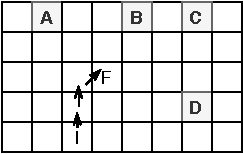
\includegraphics[width=0.5\columnwidth]{img/rg.pdf}
  \caption{The plan recognition problem}
  \label{fig:prp}
\end{figure}

Ramirez and Geffner provides a solution to the recognizer's question by accounting for the cost differences of two types of plans for each goal: (1) plans that reach a goal while going through the observations and (2) plans that reach a goal without going through the observations. Formally,
$\forall g \in \mathcal{G}: \Delta_{g} = C_g(O) - C_g(\overline{\rm O})$, where $\Delta$ refers to the cost difference, $C_g(O)$ refers to the cost of the plan that reaches goal $g$ going through $O$ and $C_g(\overline{\rm O})$ is the cost of the plan that reaches the goal without going through $O$. In the example in Figure~\ref{fig:prp}, when the agent is (\texttt{at F}),\\
$\Delta_{(at A)}= (2+3\sqrt{2}) - (3+\sqrt{2})=1.8$\\
$\Delta_{(at B)}= (3+2\sqrt{2}) - (2+2\sqrt{2})=1$\\
$\Delta_{(at C)}= (6+2\sqrt{2}) - (4\sqrt{2})=3.2$\\
$\Delta_{(at D)}= (4+2\sqrt{2}) - (3+\sqrt{2})=2.4$\\
This indicates that from the given observations, (\texttt{at B}) has the least cost difference. What does that mean? 
According to the $\Delta_g$ formula, if for a specific goal, if $C_g(O)$ is greater, it follows that $\overline{\rm O}$ is more likely than $O$ (because the rational actor agent would follow the lower cost plan). 
Putting it differently, smaller $\Delta$ means that cost of $\overline{\rm O}$ plan is greater, thus the agent is likely following the plan that is aligned with the observations. 
Therefore, given the observations, the most likely goal would be the one that has the least cost difference. 
The solution to the plan recognition problem is expressed as the subset of goals $g\in \mathcal{G}$ such that the \textit{optimal} plan for $g$ satisfies the observation sequence $O$.

How does the recognizer produce plans that are compatible with the observations? 
For this, Ramirez and Geffner use a technique called ``\textit{Compiling Observations Away}''. When the observations are compiled into the domain theory, it forces the automated planner to search for solutions that already contain the observations. 
They transform the original domain (defined in STRIPS) $D$ into a domain $D^\prime$ given the observations $O$. The new domain has the same initial state and actions as $D$. 
However, new state variable predicates are added to $D^\prime$ such that if an action $a$ is in $O$, it's definition in the domain gets added an extra state variable predicate to its post-conditions. 
This modification is done only if $a$ is the first observation in $O$. 
If there is an action $b \in O$ that immediately comes before $a$, then the preconditions of action $a$ gets added a new state variable predicate (that is already in the post conditions of $b$) and post conditions of action $a$ gets added a second new state variable predicate.

Once these modifications are done to the domain definition $D^\prime$, automated planners can be used to find plans that are compatible with the observations. $D$ is used to find plans that are not compatible with the observations. Then, to do the recognition task for each $g\in \mathcal{G}$ they compute the posterior probabilities $P(g|O) \cong \alpha P(O|g) P(g) $, where $P(g)$ is the prior probability for $g$ given as input to the recognition task and $\alpha$ is the normalizing constant. Ramirez and Geffner characterize the likelihood $P(O|g)$ as a Boltzmann distribution $P(O|g)=\frac{e^{-\beta\Delta_g}}{1+e^{-\beta\Delta_g}}$ where $\beta$ is a positive constant and $\Delta_g$ is the cost difference between observation compatible and not compatible plans for goal $g$.

\noindent\textbf{Constraints in the Approach}\\
In order to compute the posterior probabilities over the likely goals, the planner has to be invoked twice: once to find the observation compatible plans and once to find the plans that are not compatible. 
This may be costly for large problems and plan recognition in real time (i.e., when observations arrive incrementally). 
Furthermore, for the two costs to be different (and enable the recognizer to correctly identify the actor's goal) the observations must contain action landmarks for the goal we want to identify.
Landmarks are state predicates that must be true in any valid plan to reach the goal \cite{hoffman2004lm}.
Action landmarks contain the landmarks as their post-conditions. 
If the observed action is an action landmark for $g$, then $C_g{(\overline{\rm O})}$ will be higher and as a result $P(g|O)$ will be higher. If there are many ways to reach $g$ (i.e., no action landmarks) then the cost difference $C_g(O) - C_g{(\overline{\rm O})}$ will not be significantly different and as a result, it will be harder for the recognizer to identify the correct goal. 
A solution that address these constraints is proposed by E-Martin et al., which calculates the \textit{interaction} of two or more actions \cite{yolanda2015} using the \textbf{plan graph} representation of the planning task  \cite{blum1997fast}. 
They first define the cost of two proposition/actions to be established together (\textit{cost interaction}). 
This cost is propagated through the plan graph starting from the initial state until the goal states are achieved. 
The cost of achieving the goal is the sum of interactions between propositions and the costs of actions required to achieve that goal.
Like Ramirez's solution, this work also assumes that the observations are not noisy but may be incomplete.

In certain problems, it maybe difficult to provide reasonable prior probabilities for the likely goals. This is specially true in the kinds of planning domains we are working on in this research, where certain facts about the domain are hidden to the actor and the absence of complete knowledge may enable some unintended goals, regardless of their priors. For example, consider a human user unwittingly falling victim to a phishing scam because he can not recognize phishing web sites from the safe ones.

Furthermore, in certain cases the recognizer may need to recognize the actor's plan before all the observations are made available. This is also an important requirement in the domains we are studying in this research, where an agent needs to assist human users avoid certain undesirable consequences before the human user's task is completed. This requires that recognition needs to happen as observations are made available incrementally. We will discuss some recent work in online recognition in the following sections.

\noindent\textbf{Sohrabi et al. 2016 - Plan Recognition with Unreliable Observations}\\
The recognition task is similar to the probabilistic plan recognition problem proposed by Ramirez and Geffner, where a recognizer receives an observation trace of the actor's agent's behavior and attempts to identify what the actor's plan is. They also use the ``\textit{Compiling Observations Away}'' theory to generate a solution to the plan recognition problem. Sohrabi et al. propose several extensions to prior work where (1) the recognition system can now handle noisy or missing observations and (2) address observations over state variables. Further, the recognizer can identify the actor's plan and goals.

This work defines a \textbf{noisy} observation as an action that can not be explained by actions of a plan for a particular goal. \textbf{Missing} observation is an action that should have been in the observation trace but have not. When the observations are unreliable, the cost difference $C_g(O) - C_g{(\overline{\rm O})}$ will be large and as a result it will underestimate $P(g|O)$. This is because with noise in the trace, either the plan that is compatible with $O$ will have a higher cost than the plan that is not compatible with $O$ or the planner may not be able to find an observation compatible plan. To remedy this situation, they propose a new approach to ``\textit{Compiling Observations Away}'' that modifies the planning domain to include action costs; specifically penalties for noisy/missing observations.

In Ramirez and Geffner's work, the observations are presented as actual actions as defined in the domain theory. Shorabi et al. argue that in realistic examples, it may be difficult for the recognizer to observe the action itself, but he may be able to observe the effect of the action in the state. Therefore, they define the observations over state variables instead of actions. When  ``\textit{Compiling Observations Away}'', they augment the domain $D$ with special ``discard'' and ``explain'' actions. This classification helps to identify noisy observations that must be discarded. The definition for the plan recognition problem $\mathcal{R}$ closely follows from Ramirez and Geffner's definition, where $\mathcal{R}=\langle \mathcal{F}, \mathcal{A}, s_0, \mathcal{G}, O, PROB\rangle$. However, $O$ is now a sequence of states, instead of actions. Recall that the domain theory $D=\langle \mathcal{F}, \mathcal{A}, s_0 \rangle$. The augmented domain theory $D^\prime=\langle \mathcal{F}^\prime, \mathcal{A}^\prime, {s_0}^\prime\rangle$. $\mathcal{F}^\prime$ contains state variable predicates from $D$ plus the new predicates  $done, l_{o_0}$ to signal that the goal state is complete and to indicate the start of the $O$ respectively. 
In addition  $\mathcal{F}^\prime$ has a set of special predicates $l_{o_i}$ for each observation $o_i$ indicating whether the observation was discarded or explained. 
The special predicates ensure the total order of observations is maintained when the new actions are executed. 
${s_0}^\prime$ is equal to $s_0$ and has the additional predicate $l_{o_0}$. Goal $G^\prime \in \mathcal{G}$ are expressed such that $G^\prime = \lbrace done, l_{o_m}\rbrace$, where $l_{o_m}$ is the last observation. There are four types of actions in $\mathcal{A^\prime}$, each having costs associated with them \textbf{goal} action, \textbf{discard} action, \textbf{explain} action and original actions from $\mathcal{A}$. The \textit{goal action} has preconditions equal to the goal state, postcondition equal to $done$ and cost = 0. The \textit{discard action} is added when the observed state is false in the current state (i.e., observation not explained). As the post condition, the discard action adds the special predicate $l_{o_i}$ and removes the special predicate added by previous observation $l_{o_{i-i}}$. Discard action cost = $b_2$ (a application specific weight). The \textit{explain action} is added when the observed state is true in the current state. The post condition is similar to the discard action. The explain action has cost = 0. The \textit{original action} has the same pre/post conditions from the original definition $\mathcal{A}$. However, it is now assigned a new cost, which adds a penalty proportionate to the number of missing observations. The plans derived from the augmented domain theory $D^\prime$, now reflect penalties to missing and unexplained observations.

The recognition task is performed by deriving posterior plan probabilities P($\pi|O$) and posterior goal probabilities P($G|O$) following the same process as Ramirez and Geffner. 
\begin{itemize}
\item $P(\pi|O) = \beta P(O|\pi)P(\pi|G)P(G)$
\item $P(G|O) = \beta P(O|G)P(G) = \beta \sum_{\pi \in \Pi}P(\pi|O)P(G)$
\end{itemize}
$P(G)$ is an input to the recognition problem as $PROB$. Note that, now $P(G|O)$ depends on $P(O|\pi)P(\pi|G)$. Sohrabi et al. approximates this value such that $P(O|\pi)P(\pi|G) \approx 1- \frac{\beta V(\pi)}{\sum_{\pi^\prime \in \Pi}V(\pi^\prime)}$, where $V(\pi)$ is a weighted cost factor that accounts for noisy and missing observations in a plan $\pi$ for goal $G$ that satisfies $O$.  The term $\sum_{\pi^\prime \in \Pi}V(\pi^\prime)$ is computed from the sampled plans that are derived from the augmented domain theory $D^\prime$ using Top-K planner \cite{riabov2014}, which finds k-best plans and using diverse plans. The recognized goal/plan is the goal/plan that has the highest posterior probability from the set of most likely goals/plans.

\noindent\textbf{Constraints in the Approach}\\
Similar to Ramirez and Geffner's work, this solution for plan and goal recognition relies on being able to provide the goal priors as an input to the algorithm. Furthermore, the observations (although given as a sequence of states) need to be provided to the algorithm up front. For the assistive agent we are designing for human users, the recognition process needs to be separated from these constraints.

\subsection{Shvo et al. 2018 - Multi-agent Plan Recognition}
So far, we have only discussed plan recognition in situations where there is one actor and one recognizer. An extension to this paradigm is proposed in work by Shvo et al. \citeyear{shvo2018}, where the Multi-agent Plan Recognition problem (MAPR) is introduced. In MAPR the recognizer infers the goals and plans of multiple agents. The observations given to the recognizer originates from many agents. MAPR has interesting applications in multiple real domains such as intrusion detection, surveillance and so on.

When performing MAPR, the recognizer takes into account different capabilities of the agents in the domain. In addition, this work further considers actions taking some time to finish executing (durative actions). Similar to the work by Shorabi et al., observations are processed as states and not as actions. Furthermore, observations may be unreliable (i.e., contains missing/unexplainable observations). This solution to MAPR problem also builds on the plan recognition approach proposed by Ramirez and Geffner that proposes modifications to the domain theory to recognize goals/plans using automated planners. In the first step, the multi-agent aspect is compiled away into the domain theory. When there are many agents in the environment having different actions that they can execute, some actions can be executed concurrently, while others can not. They use temporal nature of actions to establish ordering constraints on the actions.  Two special state predicates are defined for actions that operate as \textit{action delimiters}: ``start'' and ``end'', which specify the pre and post conditions to the temporal action respectively. Additionally, they also define an overall precondition to the temporal action, which must hold true in every state between the ``start'' and ``end'' states. When actions are temporal, the solution plan is a sequence of action-time pairs showing actions that can execute at the same time when they are applicable.  Use of temporal actions allows concurrency of the agent's own actions as well as actions of different agents. Now, in order to compile away the multi-agent aspect, they define a privacy model for the agents when executing the temporal (and perhaps shared) actions. Action $a$ can be executed by agent $i$ if and only if $a$ is private to agent $i$ or is public to all agents. This is done by introducing special predicates to track the ownership (i.e., which agent, what objects) of state variables when a temporal action is being executed. This privacy model is added to the initial state of the planning problem. The second step is ``\textit{Compiling Observations Away}''. Here, they follow the same process as Sohrabi et al. 2016 to ``\textit{Compiling Observations Away}'' for missing and noisy observations. Then, the plan recognition problem becomes finding the posterior probabilities of plans P($\pi|O$) and  goals P($G|O$). Because the domain theory now has temporal actions, it is possible to use temporal planners to find sample solution plans.

\noindent\textbf{Constraints in the Approach}\\
The proposed approach is only evaluated for a case where the agents pursue one common goal. The assistive recognizer agent we are presenting in our research is an extension to this work. When different agents pursue different and competing goals, and when the recognizer is expected to assist one agent in the environment it needs to consider how likely the goal of the agent (who is being helped) will be threatened by competing agent(s) actions. The recognizer agent must be  able to complete recognition \textit{in time} to identify when a partial plan that seems to be helpful can be subverted by a competing agent during execution and alert the agent accordingly.



\subsection{Planning as a Tool to Model User Behavior in Cyber-security}
Cyber-security domain offers a lot of promise to study behavior both as normal users and as adversaries in automated planning. Behavioral Adversary Modeling System (BAMS) \cite{boddy2005course} uses automated planning to help computer network administrators in analyzing vulnerabilities in their system against various kinds of attacks. BAMS takes into account the properties of an adversary and produces plans that lead to system exploits that also coincides with the adversary model. While this work does not directly apply to plan recognition at its core, it illustrates a use case where classical planning can be used to design assistive systems targeted towards human end users.

This work models network vulnerabilities of a document management system as a planning problem and integrates a predictive behavior model of an adversary (who is a malicious insider) so that network administrators can concentrate on hardening the system in places where exploits are most likely and result of the exploit will be most costly. The network security planning domain contains objects such as email messages, files, hosts, user identifiers etc. and has 124 predicates to represents facts about the environment, status of tiles, capabilities, vulnerabilities of programs, knowledge possessed by users etc. Actions are represented in STRIPS with parameters, pre and post conditions. The domain has 56 actions that capture system events such as document accesses, user group modifications etc. The adversary's objectives are specified in the planning problem as goals. They use an off-the-shelf planner Metric-FF  \cite{hoffman2003ff} to find possible plans of the adversary. A graphical user interface allows end-users (i.e., network administrators) to configure problem specifications (hosts in the system, access control rules etc) and the attacker's properties (skills/tools he has) without having to encode them in PDDL.

The authors highlight several issues in modeling expressive scenarios in PDDL. 
The first constraint is the difference between the level of detail that is required in the domain and what can be modeled in the planning language. If the representation is too detailed, the resulting plans will be uninteresting and difficult for the users to extract information. Furthermore, developing and maintaining these highly descriptive domains will be a difficult task requiring expert knowledge. The second constraint is providing the plans generated by the automated planner to end-users in a natural representation. PDDL plans are not naturally comprehensible to end-users. The authors propose an encoding scheme for the PDDL actions and providing explanatory texts to capture state transitions that take place within the solution plan.

In this dissertation, we take a step toward designing assistive systems using automated planning to help human end users, who are non-experts (e.g., home users). 
Home users are specially vulnerable to undesirable consequences because they lack the know-how to recognize risky situations in advance.
A previous study \cite{byrne2016} showed that home users pay more attention to the benefits of the activities than the risk; they have goals that they want/need to achieve and are willing to take the risk to achieve them. Many triggering actions may be normal
activities (e.g., reading email, clicking on links) with the user more focused on the goal than on the risk. Thus, the undesirable consequence recognition problem needs to take into account the user’s intention as well as the undesirable consequence.

Howe et al. \citeyear{howe2012psychology} observed that most studies that look into computer security practices of users relying on self reported surveys suffered from issues such as respondent bias, socially desirable responding and peer perception.
The authors posited that experiments based on simulation, which place the participant in the actual situation that is monitored can help reduce such issues and also be leveraged to assess the emotional reactions of users to interventions and warnings.

The Intervention Problem can be directly applied in the cyber-security domain.
An attacker attempting trick the user into compromising his security/privacy during day-to-day computing tasks fits the model of the competitor we discussed in this work.
The attacker creates opportunities for phishing and malware attacks by making them to appear as common harmless tasks such as email and installing software. 
Unable to recognize these attacks in advance, the user becomes an unwitting accomplice to security breaches.


\section{Goal Recognition}
Similar to plan recognition, early goal recognition solutions involved using plan libraries. Lesh and Etzioni \citeyear{lesh1996} use a plan library based approach for goal recognition. Here, they use a data structure called a \textit{consistency graph}, which is a directed graph with actions, action schema, and goals as nodes. There is an edge between two nodes if there is a \textit{consistent} plan that supports the two nodes for some goal. Their approach to recognizing an actor's goal rely on quickly determining if a goal is inconsistent with the observed actions. Informally, the recognizer needs to conclude that the actor could not possibly have executed the observed actions as a part of a plan to satisfy the goal. This requires the recognizer to reason about \textbf{all} plans for each candidate goal. Consistency graph is an efficient way to represent planning problems and reason about them tractably.

Similar to the plan recognition problem, the goal recognizer takes as input a set of likely goals, a sequence of actions executed by the actor, actor's beliefs and a model of action schema that can be executed in the domain. The solution to the goal recognition problem is a subset of the goal schema such that, for every element in the subset, there exists a plan that achieves that goal. In order to find this goal schema subset, they first build the consistency graph. Then they gradually remove elements (action schemas/goal schemas) following a predefined rule set, which recognizes elements in the graph that are not in any consistent plan without violating the graph correctness.

Actions are removed from the consistency graph when the observed action is not consistent with other actions in the plan or the goal. This rule is sensitive to noisy observations. Oftentimes, human users do not take actions to achieve a goal in a rigid sequence. For example, they may try a few options before settling into one plan or they could just be \textit{exploring} the domain. This is specially true in the kinds of domains we are investigating in this research: cyber-security and Rush Hour. Actions generated in these type of situations may eventually be removed from the graph, which results in the recognizer failing to identify the actor's goal.

\subsection{Ramirez et al. 2009 - Plan Recognition as Planning}
This work is the precursor to the probabilistic plan recognition work proposed by Ramirez and Geffner that we discussed in plan recognition related work. There are many similarities between plan recognition as planning \cite{ramirez2009plan} and probabilistic plan recognition. As stated in the previous work by the same researchers, the environment $E$ and the recognizer's problem are defined the same. They both use the domain theory to generate two types of plans to find the most likely goal: (1) one that is compatible with observations and (2) one that is not compatible with observations.
The key differences are the assumption that the actor is only executing optimal plans and the approach they use to compile the observations away. The ``\textit{Compiling Observations Away}'' technique used in this work to modify the original domain theory $D$ into a new domain theory $D^\prime$ by adding new action definitions and predicates corresponding to the observations.

Let us define $D = \lbrace \mathcal{F}, \mathcal{A}, s_0 \rbrace$ for plan recognition problem illustrated in Figure~\ref{fig:prp}. $\mathcal{F}= \lbrace (at\:x), (adj\:x,\:y), L1\_1, L1\_2, \ldots, L8\_5\rbrace$, which indicates that the actor is at location $x$ and location $x$ is adjacent to location $y$ respectively. Predicates $L1\_1$ etc. refer to the cells on the grid, corresponding to the row and the column numbers of the cell. $\mathcal{A}= \lbrace move(x,y)\rbrace$, which indicates that the agent can move from location $x$ to location $y$. Preconditions of the move operation $pre(move)=\lbrace (at\:x)  \land  (adj\:x,\:y) \rbrace$. Post-conditions for the move operation $add(move)=\lbrace (at\:y) \rbrace$, $del(move)=\lbrace (at\:x) \rbrace$. The initial state $s_0=\lbrace (at\:L5\_3)\rbrace$. Let us assume the recognizer gets the observation trace $O=\lbrace move(L5\_3, L4\_3)\rbrace$, which indicates that the actor has moved up one cell from the initial position.

\sloppy
If we are to apply the \textit{Compiling Observations Away} theory proposed by Ramirez and Geffner to transform $D$ to $D^\prime=\lbrace \mathcal{F}^\prime, \mathcal{A}^\prime, {s_0}^\prime\rbrace$ adds one new state variable predicate such that $\mathcal{F}^\prime=\mathcal{F}\cup\lbrace p_{move(L5\_3, L4\_3)}\rbrace$ and one new action such that $\mathcal{A}^\prime=\mathcal{A}\cup\lbrace ob_{move(L5\_3, L4\_3)}\rbrace$. The new state variable predicate indicates that the an observation has occurred in the environment (in this case, move up). The new action is fully grounded and defined below.\\
\textbf{operator:} $\texttt{ob}_{\texttt{move}(L5\_3, L4\_3)}$\\
\textbf{preconditions:} $\lbrace$ (\texttt{at}$\:L5\_3$) $\land$  (\texttt{adj}$\:\:L5\_3$,$\:L4\_3$) $\rbrace$ \\
\textbf{postconditions:} $\lbrace$ $\neg$ (\texttt{at}$\:L5\_3$) $\land $ (\texttt{at}$\:L4\_3$) $\land$ $\texttt{p}_{\texttt{move}(L5\_3, L4\_3)}$ $\rbrace$\\
Comparing this to the compilation proposed in probabilistic plan recognition, the probabilistic method does not add any new action definitions to the domain theory. Instead, only the new state variable predicates are added into existing action definitions. In order to force the planner (an optimal planner in this case) to find solutions that are optimal in number of moves and also contains actions in the observations, the goals $\mathcal{G}$ are also modified to reflect the effects of the observation. For example, the goal $g \in \mathcal{G}$ such that $g=\lbrace$(\texttt{at}$\:L1\_2$)$\rbrace$ is modified to  $g^\prime=\lbrace$(\texttt{at}$\:L1\_2$)$ \:\land\: \texttt{p}_{\texttt{move}(L5\_3, L4\_3)}\rbrace$. The process of adding new state variable predicates and new actions is repeated for all actions in the observation trace. All goals in the candidate goal set are also modified accordingly. The likely goal given observations ($P(g|O)$) is found by the same calculation as the probabilistic plan recognition by taking the cost difference between optimal plans that contain the observations and optimal plans that do not contain the observations.


\noindent\textbf{Constraints in the Approach}\\
This work also has the same constraints as the probabilistic plan recognition, in that the goals are recognized when all the observations are available and the difficulty in specifying the goal priors. Plan intervention requires us to identify undesirable consequences before the task is completed. It follows that the offline model of recognition is not suitable for plan intervention. However, we will use the plan recognition with ``\textit{Compiling Observations Away}'' theory to benchmark our initial plan intervention solutions.


\subsection{Vered et al. 2017 - Online Goal Recognition in Continuous Domains}
So far, the goal and plan recognition problems we have discussed in this chapter assume the actor and the recognizer are in a discrete domain and the observations are discrete. Online goal recognition \cite{vered2017} extends the recognition problem to continuous domains. For example, in robot motion planning, we can define a simple domain as the space of possible positions for a robot. This definition can further be extended to define higher order dimensions such as angle, velocity etc. Further, the recognition is online, which means that the recognition problem must be solved for every new observation when they are revealed. The recognizer receives observations of the actor's position in the same n-dimensional space (e.g., a point or a trajectory). The recognition problem them becomes finding the goal $g$ in the candidate set of goals $\mathcal{G}$ that best matches the observations. Formally, we seek to determine $P(g|O)$ for each goal $g\in \mathcal{G}$. The recognized goal is the one that has the highest posterior probability.

They propose a new method for ranking goals in $\mathcal{G}$. Instead of taking the cost difference (Ramirez and Geffners' approach) they define a ratio $score(g)=\frac{cost(i_g)}{cost(m_g)}$, where $i_g$ is the \textit{optimal} plan to achieve $g$ and $m_g$ is the \textit{optimal} plan that achieves $g$ and includes all the observations. When the optimal plan that has all the observations is the same cost as the optimal the score approaches 1. Then $P(g|O) = \eta score(g)$, where $\eta$ is the normalizing constant. $i_g$ can be computed using a planner. To compute $m_g$, they exploit the fact that each observation is a trajectory or point in the continuous space and each likely plan is also a trajectory in the same space. Therefore $m_g= prefix + suffix$, where $prefix$ is built by concatenating all observations in $O$ into a single trajectory, and the $suffix$ is generated by calling a planner from the last observed point to goal $g$. To improve the computation efficiency during recognition, they introduce two functions: RECOMPUTE - recomputes the new plans only if the new observations seem to change the plan significantly, and PRUNE - removes unlikely goals from $\mathcal{G}$.

\noindent\textbf{Constraints in the Approach}\\
Although the recognition algorithm is evaluated in continuous domains, follow up work extends this solution to discrete domains \cite{vered2018goalrec}. The planning applications we are studying in this research are modeled for discrete domains. We will use goal ranking heuristic proposed in this solution to benchmark our initial plan intervention solutions.

The proposed online goal recognition approach further reduces the computational cost by introducing \textit{landmarks} to prune the likely goals \cite{vered2018goalrec}. 
Landmarks are facts/actions that must be true/executed at some pin all valid plans that achieve a goal from an initial state \cite{hoffman2004lm}. 
This work uses landmarks to heuristically estimate the goal completion ratio (i.e., more landmarks are active in the current state means that particular goal is closer to being achieved) as a proxy for estimating $P(g|O)$. Landmark based heuristics are often times used to improve run time during the goal recognition process. Pereira et al. use a landmark based heuristic to estimate the proximity to each goal \cite{pereira2017}. This heuristic measures the ratio between achieved and non-achieved landmarks.


\section{Recognition and Interaction}
In the goal/plan recognition  work discussed so far, the recognizer passively observes the actor. The recognizer's task finishes once the actor's goal/plan is identified. An extension to this model is to allow the recognizer to interact with the environment and affect the actor's behavior. This interaction can be \textbf{offline}: where the recognizer modifies the domain before the actor can execute any plans on it, \textbf{online}: provoke the actor to behave in some specific way by setting values of environment features, and \textbf{direct communication}: where the actor is asked questions such that the goal hypotheses can be pruned quickly. 

When designing assistive intervention models for human users, in addition to recognizing what they are trying to achieve in the domain, we must provide some guidance if it can be determined that the goal they are trying to accomplish has become unachievable. Prior work in goal/plan recognition provide some insight on how this can be achieved by allowing the recognizer to interact with the actor. We discuss some approaches below.

\subsection{Keren et al. 2014 - Goal Recognition Design}
Goal recognition design (GRD) \cite{keren2014grd} proposes a solution that allows the observer to measure the ``difficulty'' of performing goal recognition in the current domain and propose modifications (e.g. blocking actions) such that goal recognition can be done easily. GRD is an offline interaction activity, which means that unlike the typical plan/goal recognition that relies on having an observation trace for the actor's behavior, GRD analyzes the plans for possible goals in the domain an actor might execute and evaluates how distinct the plans are.

This work introduces a new metric \textit{worst-case distinctiveness} (\textit{wcd}) that measures the maximum length of the common prefix all plans for the likely set of goals may share in the current design of the domain. The solution to the GRD problem is a modified domain that assures \textit{wcd} is minimized, when plans are generated optimally. It also assumes that the actions are deterministic and fully observable.

\subsection{Pozanco et al. 2018 - Counterplanning using Goal Recognition and Landmarks}
In multi-agent settings the agents in the domain may be adversarial. This means that the agent may want to prevent another agent from achieving its goal. 
This work presents a domain independent approach for counterplanning based on goal recognition, landmarks and automated planning. 
The design of the counterplanning domain is such that there are two adversarial agents (seeking agent and preventing agent). 
The two agents pursue different goals. 
The recognizer's task is to help the preventing agent block the seeking agent from reaching his goal.

Counterplanning requires that the recognizer quickly identify the seeking agent's goal. 
This work uses Ramirez and Geffener's probabilistic goal recognition algorithm to perform goal recognition. 
Next, the recognizer needs to identify the earliest landmark for the seeking agent's planning problem (for the recognized goal) that needs to be blocked (i.e., counterplanning landmark). 
A counterplanning landmark is given a set of fact landmarks from the seeking agent's planning task, the counter planning landmark is a postcondition of an action the preventive agent can execute.
If the counterplanning landmark is a positive fluent, the preventive agent's action must delete it.
If the counterplanning landmark is a negative fluent, the preventive agent's action must add it.
The recognizer's interaction occurs when he uses automated planning to generate a plan to achieve the counterplanning landmark (e.g., negating the landmark), and therefore blocking the seeking agent's goal achievement.

\subsection{Mirsky et al. 2016 - Sequential Plan Recognition}
In goal recognition, the recognizer reasons about how likely a given set of possible goals are given the actor's behavior. The recognizer's task may fail if he can not accurately disambiguate between possible goal hypotheses. This work proposes a solution that involves the recognizer querying the actor about whether a candidate plan in one of the goal hypotheses matches the actor's intention. During the recognition process, the actor is sequentially queried in real-time whether the observed partial plan is correct. The actor's answers are used to prune the possible hypotheses, while accounting for the incomplete plans that could match with the observations after several other observations happen in the future. In order to optimize the querying process, the recognizer considers only the queries that maximizes the information-gain and the likelihood of the resulting hypotheses given the expected query result.

This solution assumes that a plan library is provided to the recognizer in advance. Their implementation of the plan library uses trees to represent the possible plans for goal hypotheses. The planning domain used in this study describes how to perform chemistry lab experiments  using an educational software that simulated a virtual lab. The plans in the planning library were traces were taken from real students' traces when interacting with the virtual chemistry lab.


\section{Behavior Classification}
The design of assistive agents for human users require that the recognizer be able to identify human behavior and how well the  behavior aligns with the goals of the system they interacts with. Human users are not always rational and may have hidden goals. It maybe an unfair comparison to model them as rational agents in real life scenarios.
 
Behavior classification is different from typical plan/goal recognition. 
It aims to achieve some insight about the actor from the passive observer's perspective. The work proposed by Borrajo et al. \citeyear{borrajo2020domainindependent} discusses the design of an observer agent, which tries to learn characteristics of other agents by observing their behavior when executing actions in a given environment. 
Using the financial transactions domain as a case study, this work models two agents: the actor (e.g., a bank customer) and an observer (e.g., the banking institution). Only the actor can execute plans in the environment. The observer does not know the actor's goal and has partial observability of the actor's behavior (actions the actor executes). Then, the observer's task is to classify the observed behavior into different types of known behavior classes. In order for the application to be domain-independent, the authors use plan distance measures (e.g., Jaccard similarity) between observed actions and distance between observed states as features to train the classifier.
Given two plans $p$ and $p^\prime$, the Jaccard similarity for the actions in the plan is defined as: 
$\frac{\left | A(p)\cap A(p^\prime) \right |}{\left | A(p)\cup A(p^\prime) \right |}$, where $A(p)$ and  $A(p^\prime)$ refer to the sets of actions in the plans $p$ and $p^\prime$ respectively.
We use a similar features to recognize the actor's plan prefixes that lead to undesirable states.



\chapter{How Do Home Computer Users Behave in Questionable Security Situations?}
\label{chap:ch3}
In this chapter, we present the findings from a human subject experiment that studied human behavior in practicing computer security.
In this study, we simulate cyber-security vulnerabilities that occur in a home computer environment when the human users perform routine tasks like checking email and using software applications. 
In our analysis, we find that the human users' intentions and post-hoc perceptions of computer security generally are not indicative of their actions; they were unaware when they had triggered security or privacy breaches.
The findings of this study motivated our work on plan intervention. 
In the next chapters we discuss three plan intervention models that can automatically detect an undesirable state developing and decide when to intervene.
Furthermore, our findings of this study support the claim that security solutions designed for end users to practice safe computing need to assess two information sources: 
\begin{itemize}
\item The human user's decision making context and the factors that affect the user's decision making ability
\item Observational data like system logs and user action sequences
\end{itemize}

\section{Introduction}
The 2016 American Community Survey found that 89\% of all households had a computer, including smartphones, making it a common feature of everyday life \cite{ryan2016}. 
Also, 81\% had a broadband subscription. 
The Internet impacts many areas of the daily life, from performing routine tasks like shopping, banking to connecting with family and friends. 
The Internet has become an avenue for pursuing formal education (e.g., online degree programs) as well as informal learning (e.g., how-to videos on cooking, household repairs etc.) and allows us to collaborate across many physical barriers. 
Whether we realize it or not, we are routinely  deciding whether or not to take risks in security and privacy when we interact with computer systems online.

Home computer use, as distinguished from work related or organizationally based computer
use, is dominated by personal activities (mostly recreational, but some financial and health related) and is not governed by security policies determined by experts. 
Most security approaches for home users encourage them to take preventative or precautionary actions, such as installing anti-virus/malware software, hardening passwords \cite{chiasson2008}, backing up information \cite{dupuis2012}. 
In this study, our objective is to understand how home computer users
make more \textit{immediate} security and privacy decisions, such as whether to click on links in email messages, to install software or visit suspect websites. 

We distinguish two decision making contexts for home computer users: unwittingly taking action that may lead to undesirable consequences (e.g., clicking on links in phishing emails) and deciding to accept the possibility of undesirable consequences (e.g., financial transactions on trusted sites or P2P software installations). 
In the first case, the user does not recognize that the situation may have undesirable
consequences. 
Thus, our research in the unwitting context will be to initially assist the user in better identifying possible undesirable consequences of action; we will do this by designing methods for automatically recognizing security/privacy risks. 
We discuss intervention solutions that address this requirement in Chapters 4 and 5.
In contexts where the user recognizes the consequence, the research will address how to help users frame their decisions: determining what alternatives are available for the user to take as next steps.
We discuss an intervention solution that address this requirement in Chapter 6 of this dissertation.


While computer security and privacy decision making share characteristics of other decision making models about possibility of undesirable consequences, the combination of decision making models within the context of practicing cyber-security is unique. 
Thus, theoretical models (e.g., Protection Motivation Theory \cite{rogers1997} and Theory of Planned Behavior \cite{ajzen1991}) applied in other decision-making contexts (e.g., health) fall short in their applicability because they use different models of risk management. 
Because of the diversity of the population and decision contexts, we favor a personalizable approach in which computer assistance can be tailored to the individual user and the decision making context.


The study discussed in this chapter makes several contributions:
\begin{itemize}
\item Analyses backed by human subject studies relating what human users think is happening to what they actually do. This is critical to understanding how much information about user's decision making context can be inferred from surveys.
\item Studies and analyses relating perceptions, actions and some user characteristics to possible interventions.
\item Software framework to support home computer user security/privacy studies. We create a lightweight, sandbox software system, which simulates the Microsoft Windows environment on desktops and laptops. The simulator supports a small set of vulnerabilities and the scenarios that could possibly trigger them.
\end{itemize}

The decision of when to flag a problem for intervention also relies on the knowledge about the user. 
We refer to this as the \textbf{\textit{user's decision making context}}. 
Success of the intervention model will depend on not bothering the user unnecessarily. 
For example, users who have the skill for recognizing computer security threats like phishing attacks, spoofing attacks and care about the negative consequences of these threats need less monitoring. 
In contrast, users who are less aware of the threats require more help. 
So, the question we need to address is \textit{what type of users make particular computer security decisions}. 
We answer this question by drawing from health related behavioral models to explain security behavior. 
Health behavior is a natural analogy to how human users respond to cyber-security threats. 
Human users frame many related issues in cyber-security using health related metaphors. 
For example, we refer to viruses and infections when talking about cyber attacks, we discuss system hardening after an attack takes place. 

The Health Belief Model (HBM) is focused on user's attitudes and beliefs. 
The user's beliefs are described based on their perceptions of six factors, susceptibility, severity, benefits, barriers, cues-to-action, and self-efficacy of performing a given health behavior \cite{rosenstock88}. 
In this work, we study the influence of two user characteristics when making security decisions from the HBM: \textit{self-efficacy}, that is an individuals confidence in her/his ability to perform a security enabling task on the computer, and \textit{cues-to-action}, that is an individual's response to external triggers for how they would affect users practicing computer security. 
We are adopting the HBM for studying user characteristics that affect computer security decision making because the HBM (specifically self-efficacy and cues-to-action) has been studied in prior work, which looked into computer security practices of the home user. 
Studies on self efficacy found that \cite{urbanska2013,aytes2004,milne2009} knowledge about how to practice safe computing increases the rate of safe behavior. 
However, having knowledge alone does not guarantee practice of computer security. 
For example, rapid advances in new security technologies make it harder for user to keep up with the latest updates that must be made to ensure safety of his computer. 
Cues-to-action triggers are advice received from external entities like friends, co-workers, media reports, laws and regulations etc. 
Studies on cues-to-action \cite{claar2010,ng2007} find that these types of cues do not have a significant effect on human users practicing computer security.  
However, these studies mainly use self-reports to evaluate the effects of self-efficacy and cues-to-action on users' decision making. 
In this work, our objective is to find out whether the same effects can be observed from human users practicing computer security in a simulated home computer environment. Furthermore, the simulated environment allows us to present cues to users that can be monitored easily such as HTTPS/HTTP web sites and safe/unsafe hyperlinks. 
This enables us to measure user responses to measurable cues as opposed to cues obtained from external sources, which are often hard to monitor and control.

Considerable research has addressed human decision making about risk. 
An individual’s risk tolerance and perception is likely to be context specific; Weber et al. \citeyear{weber2002} divided contexts into: ethical, financial, health/safety, recreational and social. 
Computer security and privacy decisions share features of several of these. 
Like some health/safety decisions, the consequences may be delayed (e.g., information theft) or unnoticed (e.g., malware), the probability of risk may be perceived as low, the actions may be routine (e.g., reading email), and the immediate primary effects (e.g., playing a new game or looking at a photo of a relative) may be recreational. 
Unlike health/safety, the cost of the threat is not as high (e.g., slow down of machine) or not as imminent (e.g., bot installed on machine). 
Like social, the user may experience peer pressure to take some action and be unwilling to admit when something goes wrong. 
Like ethical, risky actions may be violating laws (e.g., copyright in peer to peer file sharing) or putting others at risk (e.g., bots).
Additionally, the perception of cost for avoiding risk may be high (e.g., time spent learning about security), and the right actions may not be obvious (e.g., which security software to install or how best to make settings in browser). 
Moreover, given the disclosure of industry and government breaches, users may simply feel helpless.

In addition, the work by Davison and Sillence \cite{davinson2010} shows that human users' security related behavior often does not match their stated intentions. 
Human users often state the intention of being secure online but than perform actions that put their system at risk. 
Furthermore, studies that have been able to verify user's reports on their computers have uncovered lower actual than reported rates of some behaviors \cite{govani2005, national2010}. 
Therefore, developing user-friendly security solutions requires observing users performing actions rather than relying on self reporting, which acts as a proxy for actual behavior. Ideally, the home computer user should be studied at home for an extended period of time to be able to accurately gauge the computer security related behavior patterns. 
However, these requirements pose many logistical and practical problems. 
For example, the software system used in such studies should be a background process with minimal intrusion to the user's normal computing activities while collecting the necessary system/behavior information at different levels of granularity (e.g., system calls, process information, user action sequences). 
Knowledge of having these computer security monitoring software installed in their personal computers may force users to practice computer security more thoroughly than they would normally, which will lead to artificial behavior data.  
Therefore, we need to balance collecting high quality information against privacy and practicality of studies. 
The sandbox environment  we present in this chapter is designed to address the problem of collecting reliable data from human users when practicing computer security. 
Using the sandbox environment the subject is asked to walk through a protocol (task list) in a controlled environment, in which they are presented with different decisions to be made and actions taken. 
The scenarios can be designed to test the effect of cues and responses of users, thus allowing us to study computer security practices without having to only rely on self reports. 



\section{Related Work}
Before effective interventions can be developed, we must understand what types of users make particular decisions, and how they prefer to make decisions. 
What are the factors that influence user's decision making? 
Studies that have tried to answer this question have used behavioral models as a guide. Like HBM, there are many other behavioral models that have been adopted to study human user behavior such as Theory of Planned Behavior \cite{ajzen1991}, Extended Parallel Process Model \cite{witte1992} and Precaution-Adoption Process  Model \cite{weinstein2002}. 
These models define constructs that collectively represent a person's actual control over the behavior. 
Studies that apply these models to explain user behavior in computer security have looked at computer security practices such as password management, email usage, backing up data, antivirus software and firewall usage in both home and organizational environments. Typically, the studies evaluate the effects of the model's constructs on practicing security using self reported surveys from human subjects. 
We now discuss human behavior models that are commonly adopted in studies about the home computer user's security behavior.


\subsection{Modeling User Behavior for Computer Security}
Users adopting computer security concepts share many similarities with how they respond in a health related scenario. 
For example, consider a user installing an antivirus software to protect his computer against malicious. 
This is very similar to someone adopting a healthy diet to avoid diseases. HBM, developed in the 1950s after the failure of a tuberculosis screening program attempted to explain and predict health behaviors. HBM consists of six core constructs that affect an individual's core beliefs on some health related concept. These constructs are: susceptibility, severity, benefits, barriers, cues-to-action, and self-efficacy of performing a given health behavior. Let us translate the HBM for a scenario where the user is trying to protect his computer against a virus attack using antivirus software. HBM states that the user's behavior will depend on the user believing that there is a high probability that his computer will be affected by a virus (susceptibility), the user believes that the negative effect of the virus attack is a serious problem for him (severity), the user believes that having an antivirus software is helpful in preventing virus attacks (benefits), the user believes that there is little difficulty in getting a good antivirus software and using it (barriers) ,the user believes that he can recognize external trigger events indicating the computer may be at risk (cues-to-action), the user believes that he is confident in his ability to install and use an antivirus software to protect his computer (self-efficacy).

HBM has been adopted in several studies about computer security practices of human users. Ng et al. \citeyear{ng2007} study the effects of HBM constructs operationalized to the security practice of exercising care when reading emails with attachments. They evaluate the effects of HBM constructs using self-reported behavior of users. Unlike our study, which focus on home computer users, this study is conducted in the organizational context. The study finds that when exercising care while opening email attachments, self efficacy, susceptibility and benefits are determinants of user behavior. They further find that barriers, cues-to-action and perceived severity are not significant determinants of security behavior. However, they note that although the cues they have evaluated (e.g., organizational awareness programs) are not effective in prompting secure behavior in users, other types of cues could prove to be effective. In our study, we intend to address this by evaluating cues that can be presented from within the computing environment (e.g., browser notifications, secure URLs) to promote secure behavior in users.

Claar et al. \citeyear{claar2010} studies the effects of HBM constructs in the context of using computer security software anti-virus, firewall, and  anti-spyware. Like to our study, this study also focus on computer security behavior of the home computer user. Claar also extended the HBM by adding moderating variables gender, age, education, prior experience on the effect of computer software usage. Participants were recruited from university students and Internet groups and were administered a survey. The results show that self-efficacy, barriers, susceptibility influence computer security usage. This study also found that cues-to-action did not support computer security usage.

Attack graphs \cite{ammann2002} have been proposed as a methodology of modeling how a security vulnerability (goal state) can be reached starting from an initial state through a set of state transitions. Urbanska et al. \citeyear{urbanska2013} propose an extension of the attack graphs that factors in the user's interactions  with the system (in addition to the attacker) that leads to the manifestation of vulnerabilities. This state/action model is referred to as a Personalized Attack Graph (PAG). The PAG provides a basis for answering two questions related to trigger identification: (a) Which are the ``appropriate'' system states that must be monitored? and, (b) Which user actions are predicted to possibly lead to a vulnerability? A PAG explicitly ties the dependencies between known vulnerabilities existing in a standalone system and the system configuration (including characteristics of the user), to the user activities, system actions and attacker actions that can lead to an exploit of a vulnerability. The personalized aspect of the PAG comes from incorporating information about the user as \textit{user attributes}. These attributes include, user actions, preferences and assets. The authors use a Bayesian network model influenced by HBM to assign probabilities to the user attributes. User attribute probabilities for a specific user is calculated from values assigned to the six primary factors in the HBM and six additional factors (prior knowledge, experience, gender, age, socio-economic and education). However, the PAG model is evaluated using synthetic data and expert opinion. In this work, we produce actual human subject data that can be used to accurately estimate these probability values for two of the HBM constructs: self-efficacy and cues-to-action.


\subsection{Challenges in Security User Studies}
Many studies on assessing human decision making in practicing computer security including the studies cited in the previous section, report that one major challenge in conducting security user studies is the disparities between self-reported and actual observations. Howe et al. \citeyear{howe2012psychology} observed that most studies that look into computer security practices of users relying on self reported surveys suffered from issues such as respondent bias, socially desirable responding and peer perception. The authors posited that experiments based on simulation, which place the participant in the actual situation that is monitored can help reduce such issues and also be leveraged to assess the emotional reactions of users to interventions and warnings. 

Questions asked in self-reporting surveys induces respondent bias. For example in Ng et al. study \citeyear{ng2007}, the user is asked the question ``\textit{I am confident of recognizing suspicious email headers. (agree/disagree)}'' to measure self-efficacy. Users may find it difficult to estimate there skill level for some task and often times overestimate. Furthermore, asking about computer security practices primes the user for security, which may be difficult for researchers to control. A human subject study that looked into effectiveness of SSL warnings that appear during Web browsing tasks \cite{sotirakopoulos2011} attempts to minimize the priming effect by designing tasks for the Web browsers the participants normally used and simulating the same look and feel of the native Web browsers. This study also used deception. The researchers did not reveal the true purpose of the study until the tasks were completed. The results of this study also confirms that there is a disparity between self-reported  and observed actions in computer security studies. We follow the same principles in our sandbox environment design and the administering the experiment. The sandbox environment has the same look and feel as the typical Microsoft Windows Desktop. We adopted deception by presenting the participants with a cover story, which stated that we were evaluating the participants on their ability to perform day-to-day computing tasks like checking email and web browsing. We also use a combination of surveys and observational data to identify predictors of user actions. Surveys are issued to participants at the beginning and at the end of the study to more accurately gauge what the users report and what they had actually done.

While the sandbox offers a controlled environment, in situ affords realism and the ability to conduct longitudinal studies. This is particularly important in practicing computer security, which must continue beyond the initial adoption. The sandbox study we are proposing only looks into computer security practices in laboratory conditions and the study is administered only once. Accessing a user's computer in an unobtrusive way for a long period of time presents considerable challenges. Warkentin et al. \citeyear{warkentin2016} attempt to address this issue and presents a model that explains continuous intention to practice computer security. The researchers, measured the usage of an anti-malware software over nine weeks. The software was installed in the subjects' computers and usage data was sent to a web based server periodically. The study finds that in order to form an intention to continue the use of security software the effects of threat severity, susceptibility and self-efficacy are significant contributing factors.

Another challenge in human subject studies in computer security practices is the sample bias. Characteristics of the study participants vary from the general population of computer users.  Many studies use university students as the subject pool \cite{sotirakopoulos2011, warkentin2016} in order to draw a representative sample to the best of their ability. However, typical computer users are young, old, tech-savvy, non-tech-savvy, educated, uneducated, male, female and so on. The diversity of the sample should lead to more generalizable data. In our study, we also use the university students as a sample mainly because it is a sample of convenience. We however restricted the student sample to consist of non computer science majors so that we can better approximate an average home computer user.



\section{PsychoRithm: A Sandbox for Conducting Security Studies of Users}
We now present PsychoRithm, the sandbox environment we designed and implemented to study how the self-efficacy and cues-to-action impact security decision making of home computer users.
When running an experiment using PsychoRithm, the subject is presented with a desktop, which includes common applications such as emailing, Web browsing and file browsing. As the subject performs these activities, different events happen that can trigger threats and vulnerabilities of interest to the researcher. These events may include asking the user to register with a login name and a password, to provide sensitive information to gain access to a site, to respond to pop-ups asking the user to download a software. PsychoRithm records the user responses to these actions, including user clicks and time taken for response.

We had several design objectives. First, the environment needs to be as realistic as possible to encourage subjects to behave as they would on their home computers. When people are accustomed to using particular software, they have expectations about how to use it and what it will do. These expectations direct how they interact. Second, the software must be portable to different settings while also protecting the computational platform, allowing for simulation of security vulnerabilities without actually causing damage. We wanted a system that could be easily moved to a user location to run experiments. For example, if we wanted to study mature adults, we could take the setup to a senior center and conduct the experiments from there by installing the software on available platforms. Whether we run the study on someone's computer or our own, we need to retain control of the effects of the subject's actions. Yet, the possibility of infecting study machines with security experiments gone awry is very real. Given such constraints, we decided to create a fully simulated environment that would mimic the behavior of real world interaction without making any changes to the underlying operating system and minimizing changes to the file system. For example, if a pop-up asked the user to click on a button to download a software, the user would be able to click on the button, a download progress bar would show the changes, and finally a file icon would be placed in a mocked up file system browser to give the appearance that an actual file has been downloaded. Third, data collection needs to be computationally lightweight and privacy protecting. We considered a variety of methods for monitoring user interaction and found, unsurprisingly, that the most comprehensive are also the most computation intensive and potentially privacy invasive. We needed to strike a balance between carefully collecting/storing valuable data and damaging the privacy or the subject experience (e.g., not slowing down the computer so much that the subject notices). We now describe the tool we developed to support our controlled user study by first describing the user view and then the system view.

\subsection{Simulating Common Computing Activities in a Familiar Context}
Microsoft Windows is one of the most widely used desktop computing platforms accounting for 88\% of the market \cite{zdnet2020}. Thus, the look-and-feel of the Windows desktop and common applications is important to instilling familiarity for subjects. When a subject starts, he/she sees a Desktop as shown in Figure \ref{fig:desktop}. The Desktop provides application icons, e.g., a web-browser and a file-browser. Subjects can click these icons to launch the corresponding applications.

\begin{figure}[!ht]
  \centering
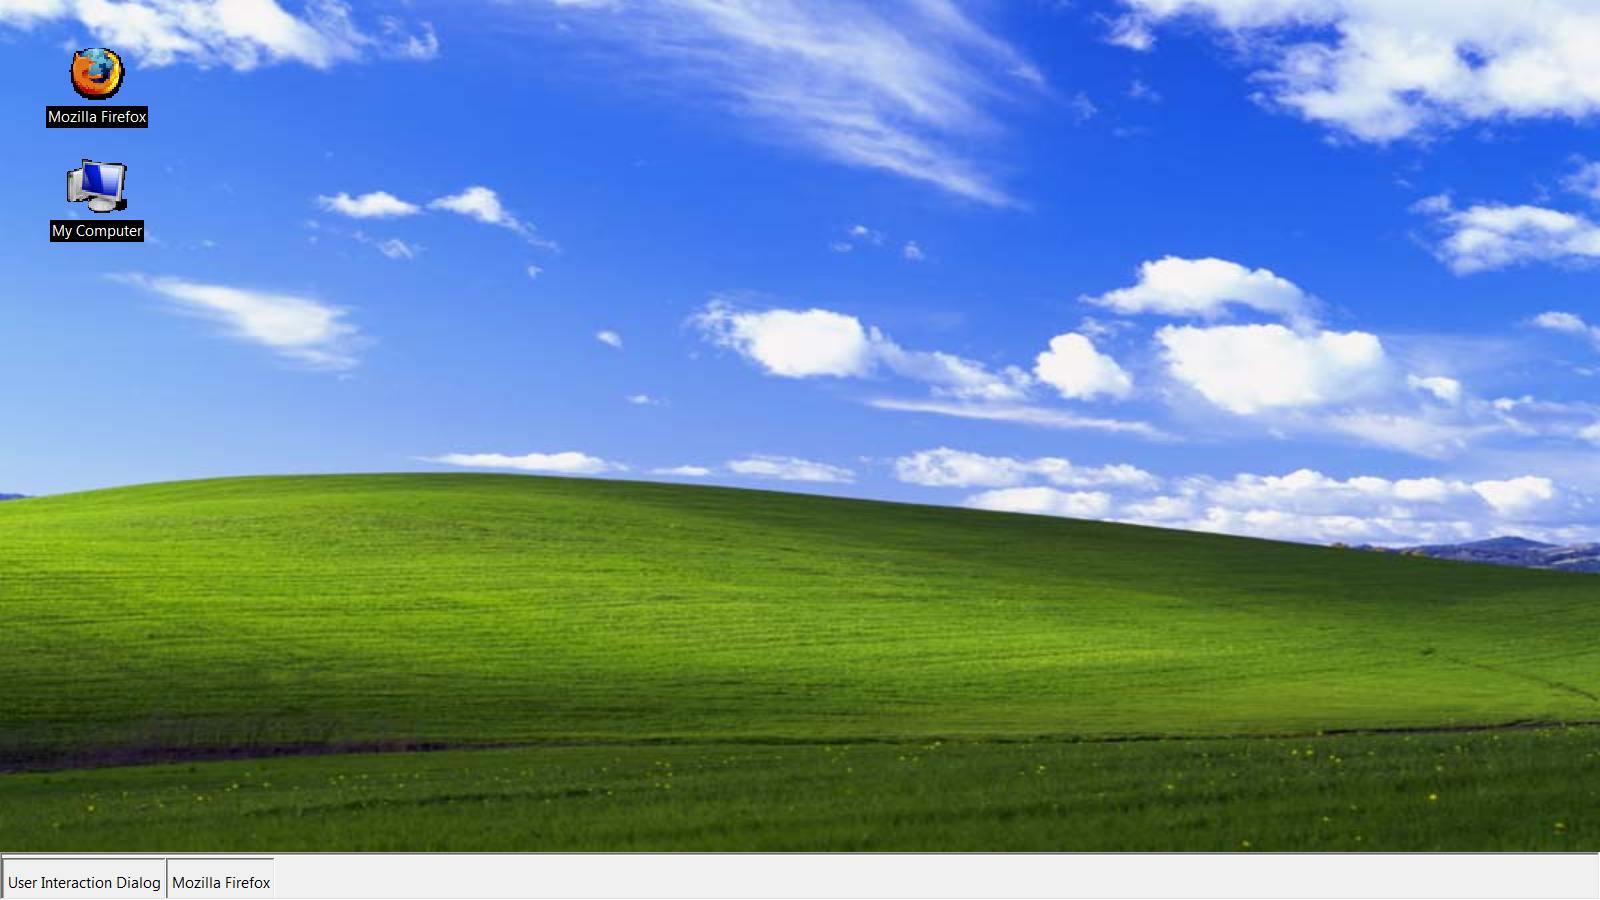
\includegraphics[width=\columnwidth]{img/desktop.png}
  \caption{Simulated Microsoft Windows desktop environment}
  \label{fig:desktop}
\end{figure}

In our study, the browser is the nexus; most of the interaction transpires through the browser. Subjects were instructed to open the browser which showed the starting page for the study (see
Figure \ref{fig:browser}). The browser not only guided the subjects through the tasks of the study, but also ensured that the subjects followed the required sequences. Subjects were allowed to perform a task only when the previous task was complete. For example, installing an application could not be skipped as subjects were required to post a verification code, which they obtained after running the application.

For the browser, we used FireFox (version 34.0.5) because it is open source, which allows us to customize the software to enable only the features we need for the simulated environment (forward/backward page navigation buttons, download button, address bar). To maintain the experience as being focused on computer interaction, web pages were used to collect pre and post interaction survey data. For our study, the data included demographic information as well as reports that could be compared against behavior as the subjects executed their tasks. To make the pages realistic, the URL bar in the PHP stub displayed the expected URLs (e.g., https://twitter.com) with an associated padlock to indicate that the HTTP connection was secure, when appropriate. The URL bar could be changed to test subject sensitivity to cues such as these. The browser also allowed for multiple tabs to be open for the experiment landing page and the various applications that are run within the browser.

Studies on global Internet users show that checking email, sending/receiving direct messages/chat, browsing for information/research and social media activities account for the bulk of the online activities \cite{furnell2007, worldinternet2018}. Thus, simulating these activities was a priority for our tool; the current version includes simulated applications of email and Twitter. Because ``google and click'' is so open ended, we did not include it in the current version of the tool.

\begin{figure}[!ht]
  \centering
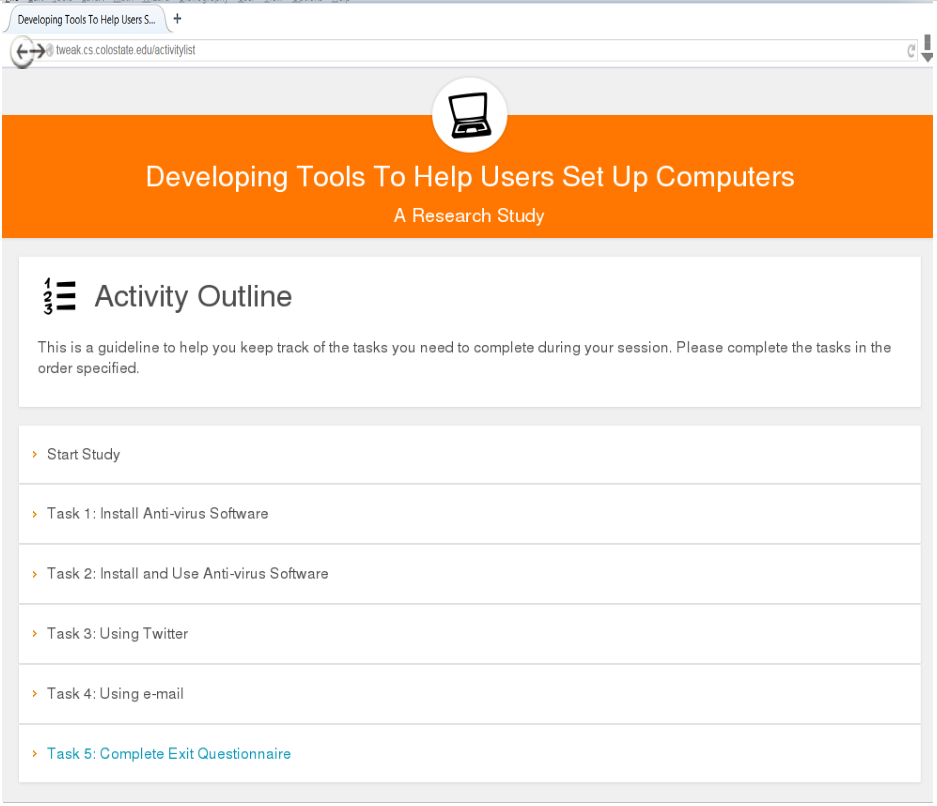
\includegraphics[width=\columnwidth, keepaspectratio=true]{img/browser.png}
  \caption{Simulated Mozilla Firefox Web browser}
  \label{fig:browser}
\end{figure}

Our email application was based off of SquirrellMail (version 1.4.22). SquirrelMail includes built-in PHP support for the IMAP and SMTP protocols and all pages render in pure HTML. These configurations fit perfectly to the technologies behind our simulated environment and therefore we could easily integrate it as an add-on service to the desktop environment. Our version of mail supports login and message functions. Subjects login using provided usernames and passwords and then can change their password. They can look at a list of messages, read and answer them. For purposes of this study, the email accounts can be populated with a set of email messages. Figure \ref{fig:mail} shows three emails that were used in our study and that were related to the other applications in the experiment protocol.
\begin{figure}[!ht]
  \centering
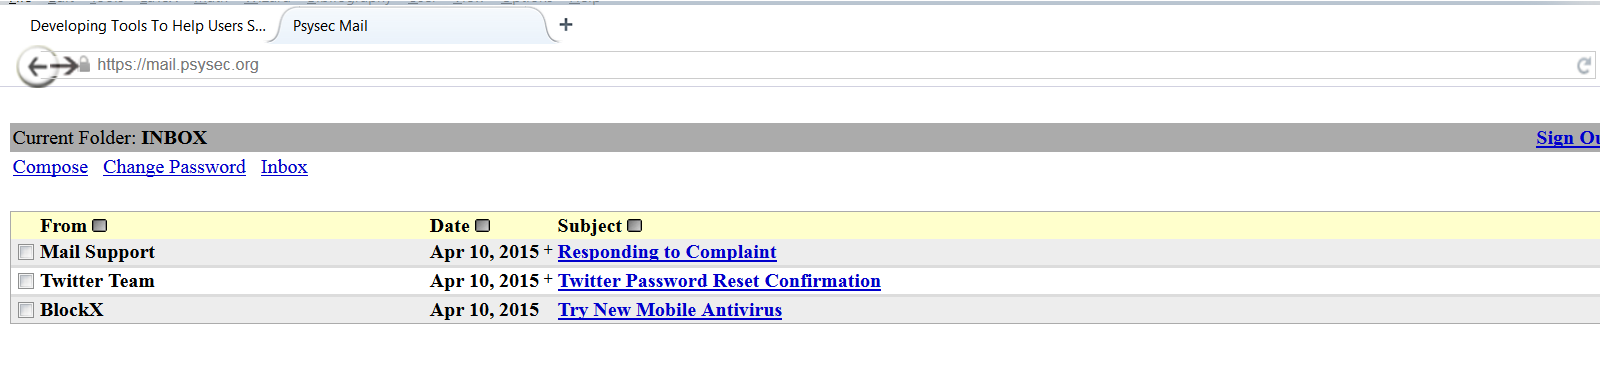
\includegraphics[width=\columnwidth, keepaspectratio=true]{img/mail.png}
  \caption{Simulated SquirrelMail email client}
  \label{fig:mail}
\end{figure}

As with email, our Twitter application supports login and message functions. Each participating user was provided with a twitter handle and a password. Three messages were posted in their respective Twitter inboxes (see Figure \ref{fig:twithome}). One of the three messages as shown in Figure \ref{fig:twitmsg}, which appears to link to a phishing website; if they click on the link, they are taken to a site which requested subjects to provide their Twitter username and password. 
\begin{figure}[ht]
  \centering
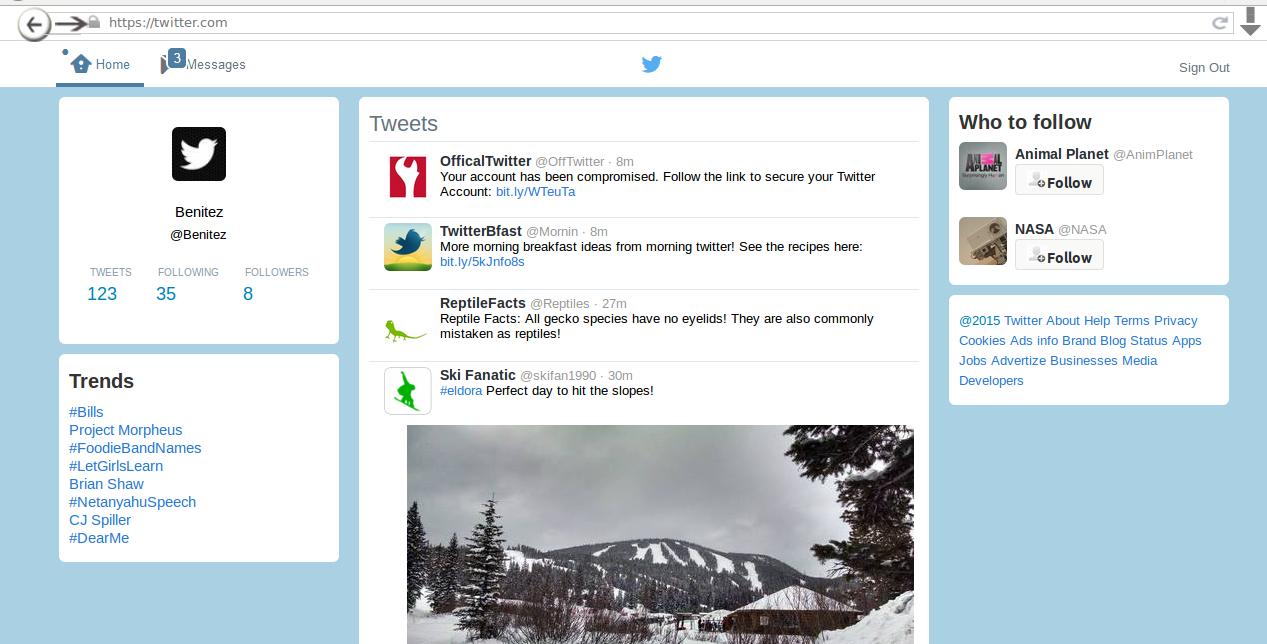
\includegraphics[width=\columnwidth, keepaspectratio=true]{img/twitterhome.png}
  \caption{Simulated Twitter home page with three direct messages in the inbox}
  \label{fig:twithome}
\end{figure}

\begin{figure}[ht]
  \centering
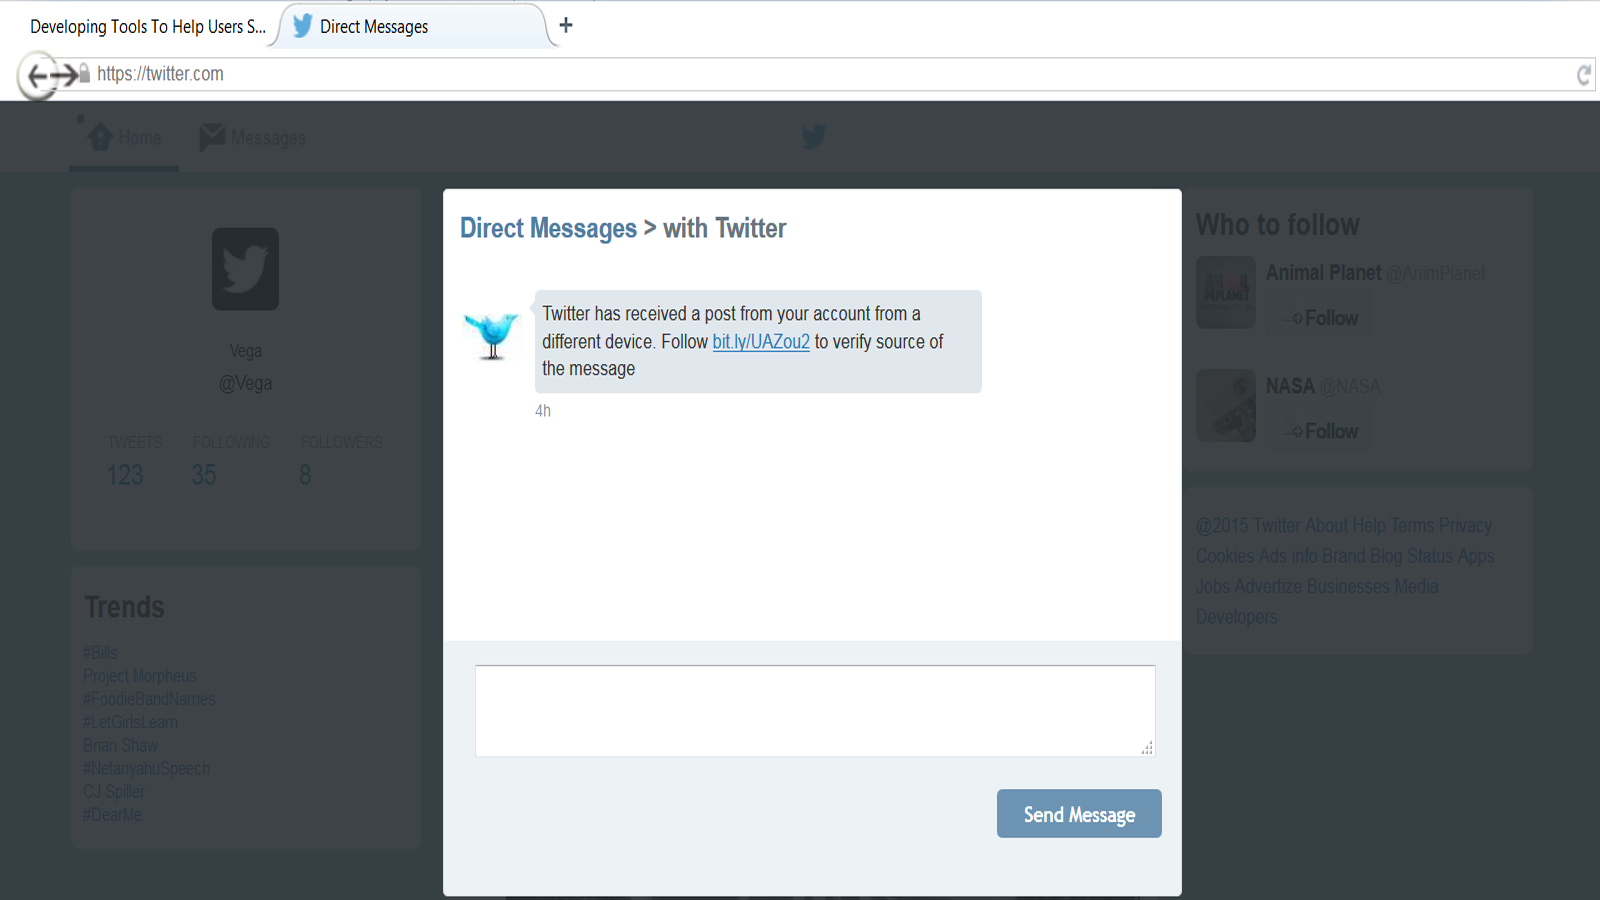
\includegraphics[width=\columnwidth, keepaspectratio=true]{img/twitter.png}
  \caption{Simulated Twitter direct message}
  \label{fig:twitmsg}
\end{figure}

To monitor the user's aptitude to use a common software application, we included an anti-virus software selection and installation activity. The subjects accessed an anti-virus download portal which leads to two separate websites as shown in Figure \ref{fig:virus}. One of the web-sites was purposefully made secure (HTTPS) while the other was made to look like a typical phishing site with flash images and dramatic warnings. Once the applications were downloaded, the subject was notified of the completed download. The subjects were then required to install and/or run the applications. To make sure the subjects installed and ran the downloaded application, the portal requested a verification code which was obtained by running the downloaded applications. Both anti-virus `downloads' were equipped with simulated system scanning capabilities (e.g., a progress bar appearing after the system scan is started).
\begin{figure}[pbt]
  \centering
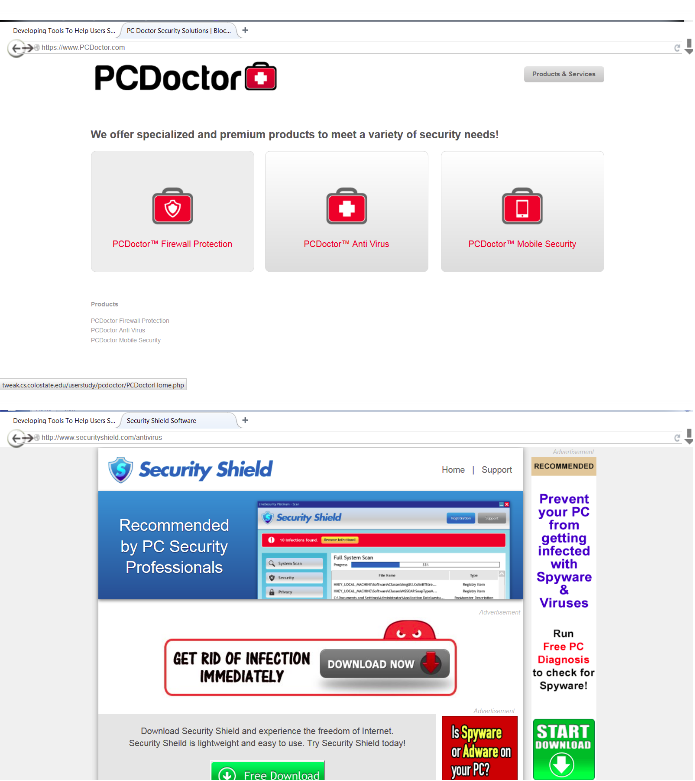
\includegraphics[width=\columnwidth, keepaspectratio=true]{img/virus.png}
  \caption{Simulated Anti-virus download pages: secure anti-virus software (top) and unsafe anti-virus software (bottom)}
  \label{fig:virus}
\end{figure}



\subsection{System Architecture}
The PsychoRithm software was designed to operate as a kiosk. The software creates a Simulated Local Environment on the subject's machine. The required applications such as the email program, the Twitter site, anti-virus software web pages, phishing web pages, and the survey questionnaires reside on the server. Software architecture diagram for PsychoRithm is shown in Figure \ref{fig:psyarch}
\begin{figure}[pbt]
  \centering
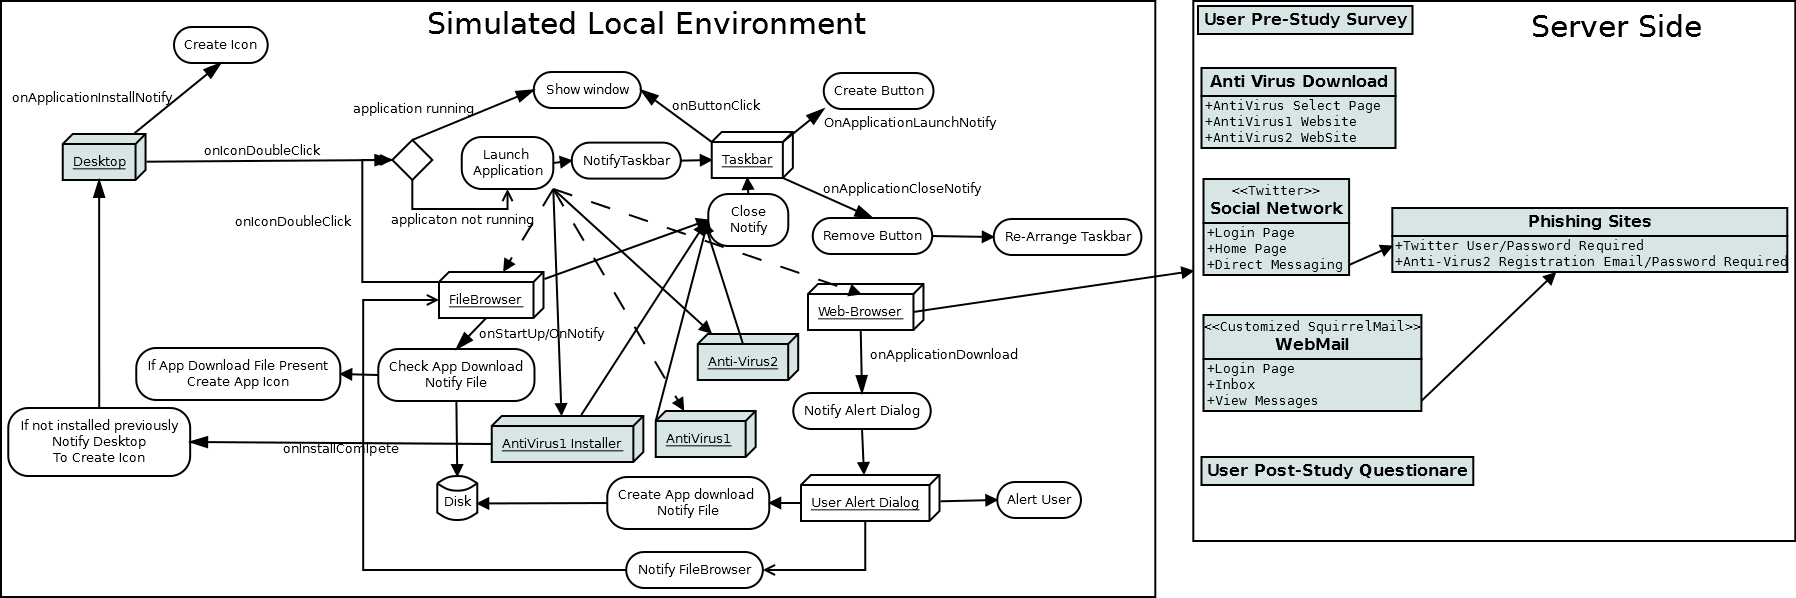
\includegraphics[width=\columnwidth, keepaspectratio=true]{img/fulluml.png}
  \caption{PsychoRithm software architecture diagram}
  \label{fig:psyarch}
\end{figure}


\subsubsection{Desktop and File System}
The user interacts with the desktop and the file system to download, install and run applications.
At the start of the experiment, the user validates his experiment username with the desktop,
and the desktop creates a folder specifically for that user. The simulated desktop provides application icons: Mozilla FireFox Web browser and the My Computer file browser (Figure \ref{fig:desktop}). The user can click these icons to run the corresponding application. When new applications are installed, such as the anti-virus software, new icons are added to the desktop. The desktop and all applications are supported by a taskbar, which provides easy access to all opened applications.

To make the simulated desktop resemble a real desktop, we implemented it as the topmost Win32 Tool Window spanning the working area of the actual desktop. Underneath the simulated desktop is an invisible list-view window, which hosts the application icons. Inter-process communication was performed using custom defined messages with application specific WPARAM values. We implemented our own opaque taskbar as a Win32 Toolbar that maps a zero-based incremental index to the launched applications. This index was used to track buttons/window-handles and close/rearrange them when applications were closed.

PsychoRithm was built as a package that contained empty folders like the \textit{Downloads} and \textit{LoginData}. It was placed under the \verb|C:\Users\<login_name>\Documents}| directory (to avoid conflict with system directories) and identified with \verb|login_name| on the fly to create the absolute path to the package. However, since the path was created dynamically, we could not configure the exact location of the \textit{Downloads} folder into Firefox and hence used the \textit{User Alert Dialog}. A Win32 window with an underlying list-view was used as the file browser for the \textit{Downloads} folder.


\subsubsection{Web Browser}
The Web browser component allows the user to browse the content fetched from the server. To create the illusion that applications were downloaded from a specific URL, we disabled the Firefox warning dialog by editing the mimeTypes.rdf which led to Firefox calling the User Alert Dialog. Similarly, to make websites like Twitter appear to be served from twitter.com, we removed the URL bars from the existing Firefox application and introduce a custom PHP stub (enabled with Javascript navigation functions) which emulated a URL bar and allowed subjects to navigate/reload pages in same browser session. This required mocking up images that made the interface appear as expected and means that any visited URL must have a corresponding image to be loaded. Action login was facilitated by PHP session variables and AJAX event handlers.

All widgets were disabled using a FireFox extension. When subjects double-clicked on the Firefox icon, the Firefox window was brought above the simulated desktop window giving the illusion that a new application has been launched. A custom designed Firefox extension allowed subjects to minimize this window, but not quit it.

\subsubsection{Email}
The SquirrellMail portal ran on top of a DoveCot IMAP/POP3 server.

\subsubsection{Anti-virus Applications}
Two anti-virus applications were created using Java Swing Platform. One of the anti-virus applications requires installation. After installation, it notifies the Desktop, which then creates an icon
to launch the application. To make the download process realistic, the web browser makes a call
to the \textit{User Alert Dialog}, which then alerts the user, creates a 0 byte file in the Downloads folder
and notifies the file browser.

\subsubsection{Collecting Data}
The system is instrumented to collect subject actions, specifically the start and conclusion of the session, the activation of each activity, typing and mouse clicks in the applications (buttons, widgets, windows, etc.) The results of the pre and post surveys and subject preferences (e.g., software selections, password choices) were also logged using PHP session variables. All activity related data are captured with timestamps. Once the experiment is complete, the Desktop
process sends over all captured data to the server side using SFTP/SCP, cleans all of the local storage and kills any process that was initiated by the system.

As per the regulations of the Institutional Review Board (IRB) of the Colorado State University, the researchers are required to store subject data in a safe and secure manner. Moreover, to run enough subjects, we needed to allow multiple subjects to participate simultaneously. Consequently, a secure remote server also stored experiment data in a safe manner. To preserve anonymity, the data were associated with the IDs (login names), which were assigned randomly when subjects arrived for the study and were never associated with specific individuals.

\subsubsection{Configuration and Extensions for Other Studies}
Microsoft Windows and Visual Studio Framework are required to install and use PsychoRithm. The web applications (Twitter, Software download pages are implemented using HTML/AJAX/JQuery. The Anti-virus mock-up software is implemented using Java. For this study, the simulator only supports Web browsing (restricted only to predefined URLS), file browsing (restricted only to personalized \textit{Downloads} directory) and email (restricted only to SquirrelMail webmail application) applications. Access to other Windows applications are restricted through the simulated desktop and the web application shown in Figure \ref{fig:browser}. 

Because Firefox is an existing application, it must be started at the beginning of an experiment session and cannot be stopped during the course of the experiment. As a result, the subjects were only allowed to minimize the application and restore it via the taskbar button. All menu operations, including right-click menu operations, were disabled. In this study, our main focus is on evaluating users' behavior with regard to self-efficacy and cues-to-action while performing common tasks on the computer. There are other behavior models, which describe many other factors that affect user's computer security behavior. In situ evaluations for these factors may require simulations for additional, more complected tasks. In this case, future add-on Windows applications can be developed using the aforementioned technologies and integrated as plug-ins.


\subsection{Studying Behavior In Situ}
The goals of this experiment are:
\begin{itemize}
 \item capturing actions taken by users when asked to perform tasks that provided ``opportunities'' to trigger security vulnerabilities
 \item characterizing their behaviors by their gender and prior experience
 \item assessing consistency in subjects answers
and actions.
 \end{itemize}
In this study our focus was on two factors common to several well-known models of user security behavior: self-efficacy and cues-to-action (e.g., Health Belief Model, Protection Motivation Theory). The core idea was to ask questions related to those two factors, then observe the user actions within scenarios designed to elicit potentially detrimental responses and then to ask questions about the tasks that they had undertaken. This protocol was designed to collect data on how the two factors manifest in the participant sample and to allow us to compare the self reports of against the observed actions. While we had no hypothesis about how the factors would appear, our hypothesis about the comparison of data collection methods is that self-reporting was likely to differ from observed actions. Thus, the study was designed with five parts: an introduction, a pre-study questionnaire, on-line completion of four tasks, a debriefing and a post-study questionnaire.

The sandbox software allowed us to analyze the actual behavior of human users when they are presented with scenarios that may lead to serious computer security exploits such as installing illegitimate software, responding to phishing email, not changing default passwords, potentially in contrast to what they report in a survey. If the participants were directly informed of the real purpose of the study (i.e., computer security practices), it is likely they would be extra cautious in completing the tasks. This self-consciousness could influence what they do in the experiment making it differ markedly from their actions outside the context of the research study (e.g., at home, workplace) and introduce an additional bias to measurements we collect. To this end, we introduced some deception into the study in three ways:
\begin{enumerate}
\item The description of the study used to attract participants indicated that the study was to evaluate their ability to complete common tasks on the computer so that the researchers can
use the findings to develop tools to help users set up their computers.
\item A task, which was unrelated to the focus of the study (i.e., compose and save email as draft)
was added to one of the other tasks to help mask the actual purpose of the study. This task
did not generate any useful data.
\item To induce a sense of buy in, the participants were presented with a cover story at the start of
the study. The cover story stated that the participant had purchased a second hand computer
with Microsoft Windows and one utility application (Mozilla Firefox) installed. Experiment tasks were to study the participants ability to set up this newly purchased computer to be used as an additional computer by multiple users at their home. The cover story was
communicated to participants during the introduction session.
\end{enumerate}
During the debriefing session, participants were informed of deception used in this study. The study was designed as a within-group experiment, where all participants were placed in identical threat scenario simulations. Written instructions were given to all participants to assist them in completing the required set of tasks. All data were collected through the PsychoRithm sandbox. Text computer logs recorded the tasks that were completed, timestamp at which a task was completed, the selections made when options were presented, external URLs visited by following links on web pages, and updates made to user visible settings. Video/audio recordings were not used. The study took approximately 45 minutes to complete.


\subsubsection*{Participants}
In Spring 2015, we collected data from 61 university undergraduates as participants. The students were enrolled in a psychology course during that semester. The course attracts a wide range of majors and gives research credit for participating in studies. All participants were given informed consent and participated voluntarily.

Although selected as a sample of convenience, the sample was representative of home computer users from a critical group: young adults with easy access to computers. Prior studies have shown that high school and college aged adults, age between 18 and 34 report the highest level of Internet usage \cite{census2012}. 56\% of participants in this study were female. 74\% were less than 20 years of age, 25\% were aged 20-25 years and the remaining participant was aged 26-30. 98\% were working toward a Bachelor's degree.

\subsubsection*{Surveys}
We presented two surveys. The pre-study survey shown in Appendix \ref{apx:cypre} asks three questions (questions 1 - 3) about demographics and 10 questions about computer experiences (questions 4 - 13). Although we would have liked to directly assessed self-efficacy, the standard questions, as pioneered by \cite{ng2007, claar2010}, asked about level of confidence when executing specific tasks in different contexts. We did not wish to prime the participants to be thinking about computer security during the on-line portion of the study. Instead, we followed the tone of Mannan and van Oorschot \cite{mannan2008}, which asked about their experience with computers (questions 4 - 8), what challenges they perceive (question 9), where they obtain help (questions 10 - 11) and what software they have installed (questions 12 - 13). These questions were selected to relate more clearly to the cover story.

For the post-study survey shown in Appendix \ref{apx:cypost}, we adopt the standard survey instruments, which evaluate self-efficacy for computer security practices from \cite{ng2007, compeau1995}. Instruments that measure cues-to-action are adopted from \cite{ng2007}. It must be noted that our idea of cues refer to security notifications available in the computing environment such as SSL lock icon in URLs, web site content/look and feel as opposed to external information sources like news, help-desks etc. in Ng et al.\cite{ng2007}. Questions 2 - 11 evaluate the self-efficacy of the anti-virus software usage. Questions 12 - 19 evaluate self-efficacy of safe communication over social media (Twitter). Questions 21 - 24 evaluate self-efficacy of using email and managing passwords. Questions 20, 25-29 are about awareness of secure and private information collection. Questions 30 - 35 evaluate cues-to-action on practicing computer security on the Internet. The first question asks for the pseudonym which allows us to connect the on-line portion's data with the post-survey data. The main purpose of these questions was to establish whether or not the actions in the online portion of the study corresponded to what they thought that they did.


\subsubsection*{Experiment Procedure}
When the participants arrived for the study, one person checked their name on an attendance list, and then another person had them pick a persona ID from folded slips of paper in a basket. The persona ID included a fictitious name, user ID and password to login to the simulated desktop. All data were collected using the persona ID, which was never connected back to the participant's actual name. They were then led to a computer and assisted in logging into the kiosk software.

The starting page provided the instructions to the participants. To avoid alerting them to security issues, we presented the cover story below for what they were being asked to do.

\begin{center}
\framebox{%
  \begin{minipage}{0.8\columnwidth}
    \setlength{\parindent}{25pt}
    You have just bought a second-hand desktop computer from Surplus Property, the recycle, reuse sales point of Colorado State University. This computer will be used as an additional computer at home. The computer already has Microsoft Windows operating system installed. Notepad, Windows Media Player and Mozilla Firefox web browser are installed as application software. Additionally, you also managed to get an Internet connection setup for the computer. This computer will be used by you and your family members for regular purposes such as checking email, browsing Internet, and also for entertainment activities like watching movies and videos.
    
  \setlength{\parindent}{25pt}
This study helps us understand your ability to perform common tasks on a computer, while it is being set up. To familiarize yourself with the new environment, you may browse the computer and check what applications are installed. Please note that, for the purpose of this study, a custom desktop environment was created and therefore it may not have all options available in a typical desktop computer.
\end{minipage}}
\end{center}

\vspace{1em}
The participants were presented with a screen that described and organized their on-line tasks. This page was generated as the participant finished one activity and moved on to the next. They were first directed to take the pre-study survey. Their last task was to complete the post study survey. The online portion presented three threat scenarios: (1) selecting, installing and using an antivirus software to ensure safety of the computer, (2) communicating on social media and (3) using email.

In the first scenario, participants were directed to install, configure and run anti-virus software as part of setting up their new machines. Below is the the instructions that were presented to the user as they started these tasks.
\begin{center}
\framebox{%
  \begin{minipage}{0.8\columnwidth}
  \textbf{ Task: Install Anti-virus Software}\\
  \setlength{\hangindent}{15pt}
	\textit{Please read the following description before you begin}
	
	\textit{You may have noticed that the computer does not have any anti-virus software installed. You are concerned about this lack because the computer will be shared among your family members. Your  task is to install and configure an anti-virus software to be used in this computer. Names of software you will see during tasks are fictitious.}

	\begin{itemize}[topsep=8pt,itemsep=4pt, parsep=-4pt]
	    \item \textit{On ``Study Road Map'' web page click ``Install Anti-virus Software'' Link. You will be directed to a page with two anti-virus program options: \textbf{PCDoctor}, and \textbf{Security Shield}}
    \item \textit{Read the descriptions given for each software}
    \item \textit{Choose ONE anti-virus program. On clicking ``Visit web page to Download Now'', you will be directed to software provider's web page.}
    \item \textit{Find the correct download link on the provider's page. }
    \item \textit{Click on the correct download link to automatically download the software onto your computer.}
    \item \textit{Run installation wizard to install the software on your computer.}
	\end{itemize}

\end{minipage}}
\end{center}

Two antivirus software installations were offered via a web-based download portal implemented within PsychoRithm. One software was designed to be legitimate and safe; the other was intended as suspect and insecure. Neither were existing products or websites; in each case, we patterned our fictitious web pages after exemplars of each type of antivirus software website.  The legitimate software is ``PCDoctor'', and the suspect one is ``Security Shield''. The portal provided a brief description about each software program to assist users make a decision about which program to download. Once the software was downloaded, users were given written instructions to install the software, configure it to enable three additional security features (automatic live updates, removable media scan, and smart firewall) and finally perform a simple scanning task on the computer. Although neither program actually did anything, both were designed to give the users the interaction experience of an authentic antivirus program with appropriate timing pauses and messages (see Figure \ref{fig:rogueav}).  

\begin{figure}[!pbt]
  \centering
  \subfloat[System scanning]{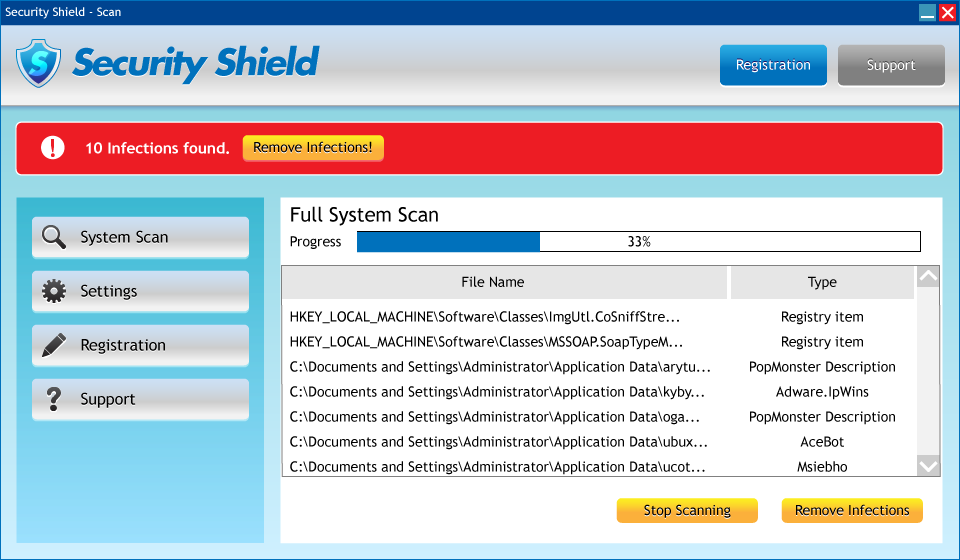
\includegraphics[width=0.5\columnwidth]{img/av1.png}\label{fig:scan}}
  \hfill
  \subfloat[Anti-virus protection settings]{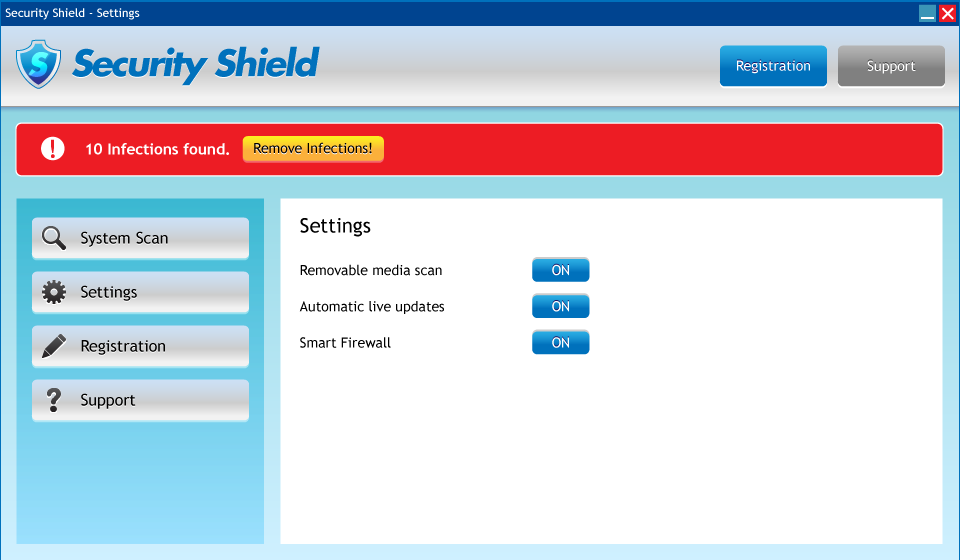
\includegraphics[width=0.5\columnwidth]{img/av2.png}\label{fig:settings}}
  \caption{Security Shield anti-virus mock-up software}
  \label{fig:rogueav}
\end{figure}

A mock-up version of a popular social media application (Twitter) was implemented for the purpose of studying users' communication habits. In this activity, users were instructed to use a private messaging feature of Twitter. In this case, we did create an version of the interface for the specific media site because it corresponded well with the cover story and we were interested in their behavior within this likely familiar context. Users were shown three private messages: two legitimate, safe messages sent from trustworthy sources (different offices within the university at which the study took place) and one phishing message. As shown in Figure \ref{fig:twitmsgall}, all messages contained URLs. The URL in the phishing message, directed users to a phishing website \texttt{bit.ly/UAZou2}. Once the users visited the phishing website, they were prompted to enter their username and password. In their instructions, they were told that this task would allow them to check that Twitter was working correctly on the computer; they were asked to login, read messages and ``take appropriate action''.

\begin{figure}[pbt]
  \centering
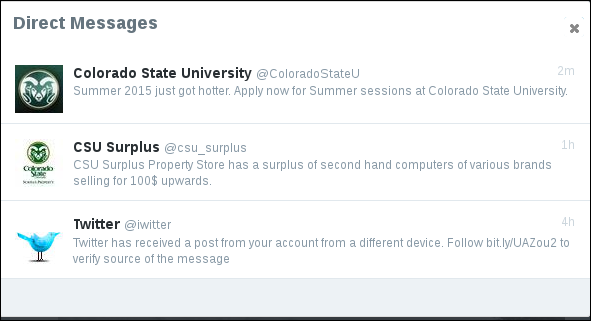
\includegraphics[width=0.7\columnwidth, keepaspectratio=true]{img/twittermsgs.png}
  \caption{A screenshot of the messages as they appeared to the participants}
  \label{fig:twitmsgall}
\end{figure}

A web based email client was used for the email scenario. Users were given personal email accounts and a common default password designated for the study. They were told ``The email account is unique to you. However, the default password is being shared by all users of the computer.'' The email task comprised two sub tasks. First, to study their ability to choose strong passwords, participants were instructed to change the default password of their email accounts to a new password of their choice. Second, users were instructed to compose a new email message, read email messages and respond to unread messages.

As shown in Figure \ref{fig:emails}, three new messages were placed in the inbox: one safe message and two unsafe messages. One of the two unsafe messages was a phishing message with a URL that would direct the user to a phishing website upon clicking. The phishing website was masked as the web-mail client itself. The other unsafe message contained an attachment: a harmful zip file. The message content was patterned after actual phishing email messages. The phishing websites and zip file attachments were mock-ups within the sandbox; thus, they did not pose an actual security threat to the computer or to the participant's personal data. 
\begin{figure}[htb]
  \centering
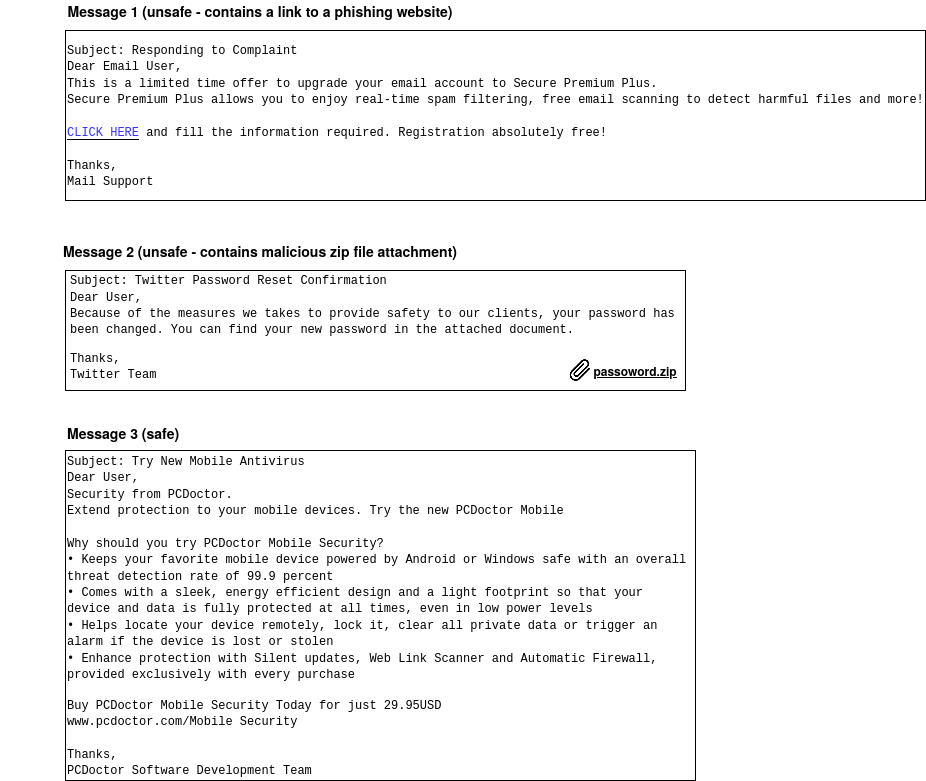
\includegraphics[width=\columnwidth, keepaspectratio=true]{img/emails.png}
  \caption{Email messages presented as part of the online portion of the study.}
  \label{fig:emails}
\end{figure}

We designed the phishing website to follow examples we had seen before and also placed several cues in line with commonly recognized properties of online phishing attacks \cite{ftc2019} for both the social media phishing attempt and email phishing attempt. First, in the case of Twitter, although the message sender's name was ``Twitter'', the Twitter handle (i.e., message sender's twitter account name) was not similar to the legitimate Twitter account's Twitter handle. The legitimate account's Twitter handle is \texttt{@Twitter}. The phishing message was sent from the Twitter handle \texttt{@iwitter} (i.e., Twitter misspelled). Second, the message said that some log-in attempts have been noticed. Third, the message content requested that the recipient confirm some personal information, specifically the user's Twitter account user name and password. If the user failed to recognize these cues and clicked on the link, the user is directed to a web page, which contains a log in page but looks different from the legitimate Twitter log in page. Users had already seen the legitimate log in page at the start of the Twitter task and ideally should be able to recognize that the current web page is different. We added several cues to this page as well. We changed the Twitter logo and the color scheme of the phishing web page. The URL did not contain the SSL lock icon and was \texttt{http://iwitter.com}, whereas the legitimate web site's URL was \texttt{https://twitter.com}. If the user did not recognize the phishing web site given all these cues and submitted the user name and the password, the user was directed to a landing page, which displayed a message that the user's personal information has now been compromised. Then the user was directed to the next task.

A similar approach was taken to handle security attacks that occur via email. The phishing message on email was masqueraded to appear as if it was being sent by the Anti-virus software vendor. Recall that, in the sequence of tasks, when the user reaches the email task, they would have already completed the anti-virus task and is familiar with the Anti-virus vendor's name. We embedded the same discrepancies between the legitimate vendor's information and the phishing website as the Twitter phishing scenario as cues for the email phishing use case. If the user clicked the phishing link, the same sequence of events took place as in the case of the Twitter phishing scenario. There were several cues to recognize the malware email such as the generic greeting from the sender (``Dear User''), an enticement to open an attachment (get the new password by opening the attachment), information review check (password change) and undisclosed recipient (``Mail Support''). If the user clicked the attachment, the user was directed to a web page, which displayed a message that the computer system's safety is now compromised.


Once the participant finished the tasks, he/she was directed to the post-study survey and a
debriefing explanation. We also offered them the opportunity to further discuss the debriefing with one of the staff conducting the study.


\section{Data Analysis and Results}
This study has two main components that evaluate users' computer security behavior: self-report surveys and the sandbox activities. Therefore, we divided the analysis as within component (only surveys and only sandbox) and across component (surveys and sandbox). We first present the analysis on single components.

\subsection{Pre-Survey Findings}
Table \ref{tab:cypre} shows a summary of the pre-survey findings. Although the participants had a lot of prior experience with computers (66\% with more than 9 years), they had little formal training (59\% had none) and turned to the Internet for help as their primary source (92\%). Most (82\%) owned multiple devices. Nearly all (95\%) had installed multiple applications, i.e., Chrome, Office, Flash, Skype and Acrobat. Given the participant recruitment method, it was not surprising that nearly all had laptops and used their computers for educational activities. With respect to computer security, more than half (67\%) found it challenging to identify harmful actions and take steps to ensure safety. Yet most (77\%) had anti-virus software on their computers.

\begin{table}[ht]
 \resizebox{\columnwidth}{!}{
\begin{tabular}{|ll|}
\hline
Years experience &
  4-6: 11\%, 7-9: 23\%, \textbf{\textgreater 9 : 66\% }\\ \hline
Usage hrs/day &
  \textless 3: 30\%,\textbf{3-6: 54\%}, 7-10: 11\%, \textgreater 10: 5\% \\ \hline
Devices &
  \begin{tabular}[c]{@{}l@{}}\textbf{laptops: 97\%}, smartphones 82\%, tablets: 33\%, desktop PCs: 21\%, \\ e-Readers: 7\%, Other: 3\%\end{tabular} \\ \hline
Applications &
  \begin{tabular}[c]{@{}l@{}}\textbf{web browser: 98\%}, Office: 82\%, Acrobat: 61\%, Media Player: 49\%, \\ Computer Games: 26\%, \\ Image Processing: 21\%, Software Development: 11\%, Other: 3\%\end{tabular} \\ \hline
Purposes &
  \begin{tabular}[c]{@{}l@{}}\textbf{Education: 93\%}, Documents: 84\%, Communication: 82\%, Entertainment:\\ 82\%, Information gathering: 74\%, Financial: 56\%, Work: 41\%, Games:\\ 26\%, Programming: 10\%\end{tabular} \\ \hline
Challenges &
  \begin{tabular}[c]{@{}l@{}}\textbf{Identifying actions that may harm the computer: 67\%}, Taking steps\\ to ensure the safety of the computer: 51\%, Installing, configuring and getting\\ a software application ready to be used: 43\%, Finding application software\\ that matches my requirements: 39\%, Finding and using help manuals: 25\%\end{tabular} \\ \hline
Training & 
\begin{tabular}[c]{@{}l@{}}\textbf{None: 59\%}, Application Courses: 21\%, Programming Courses: 13\%, \\ On-line Tutorials: 5\%, Face to Face Classes: 2\%\end{tabular} \\ \hline
Help sources &
 \textbf{Internet: 92\%}, Friends: 54\%, Relatives: 46\%, Local Stores: 23\% \\ \hline
Anti-virus usage &  \textbf{Yes: 77\%}, No: 23\% \\ \hline
Installations &  \begin{tabular}[c]{@{}l@{}}\textbf{Google Chrome: 89\%}, Office: 85\%, Flash: 75\%, Skype: 62\%, Acrobat: 57\%, \\ Firefox: 33\%, QuickTime: 25\%, VLC Media Player: 21\%, Thirdparty email: 10\%,\\ Other: 7\%, Opensource Office: 3\%\end{tabular} \\ \hline
\end{tabular}
}
\caption{Summary data from the pre-study survey questions. Each row is a question with its number and short description. Highest values in each row are in bold.}
\label{tab:cypre}
\end{table}


\hspace*{-18pt}\textbf{Gender and Computer Usage Patterns} 

We analyzed the data to identify any differences that may appear between male and female participants. For questions that could be coded as numbers, we ran
two sample, two tailed T-tests. For questions that had categorical answers, we constructed $2 \times R$ contingency tables, where $R$ was the number of categories, and ran Pearson's chi-squared tests. All analyses were performed using the R statistical package. 

Table \ref{tab:cypregender} shows the results for gender on questions 4, 5, 6, 7, 9 and 13. We coded years of experience (question 4) as 5 for 4 - 6 years, 8 for 7-9, and 10 for $>$ 9. We coded hours/day (question 5) as 2 for $<$ 3, 4.5 for 3 - 6, 8.5 for 7 - 10 and 11 for $>$ 10. For questions 6, 7, 9 and 13, we counted the number of answers given by each participant. Although the means on each of these questions shows some differences between female and male participants, that difference is significant for only one question: the number of challenges. The female participants reported 2.68 on average, where the male participants reported 1.70. Thus, the perception of self-efficacy in computer usage for the females was clearly lower than for males.

\begin{table}[ht]
 \resizebox{\columnwidth}{!}{
\begin{tabular}{|l|l|l|l|l|l|l|}
\hline
                    & Yrs Experience & Usage hrs/day & Devices & Applications & Challenges & Installations \\ \hline
Mean Female         & 8.88           & 4.81          & 2.50    & 3.55         & 2.68       & 4.59          \\
Mean Male           & 9.07           & 4.20          & 2.33    & 3.70         & 1.70       & 4.74          \\
p-value \textless{} & 0.66           & 0.33          & 0.53    & 0.69         & 0.002      & 0.73          \\ \hline
\end{tabular}
}
\caption{Comparing male and female participants on questions coded as numbers, Rows show mean
for females, mean for males and p value for T-test.}
\label{tab:cypregender}
\end{table}

Questions 6 - 13 had categorical answers. For these, we used each of the pre-specified answers as categories. We had few cases in which ``Other'' was used and so did not include that as a separate category. Table \ref{tab:cypreusage} summarizes our findings. The last column lists the category that showed the largest percentage difference and lists the percentage after the category name. For installs, no females and only 2 males installed OpenOffice, so we did not list it as the largest difference.

\begin{table}[ht]
 \resizebox{0.7\columnwidth}{!}{
\begin{tabular}{|l|l|l|l|l|}
\hline
Question      & \( \chi\)& df & p \textless{} & Largest Difference               \\ \hline
Devices       & 5.58                & 4  & 0.23         & Desktop PC -21.6                 \\
Applications  & 5.69                & 6  & 0.46         & Computer games -26.0             \\
Purposes      & 8.44                & 8  & 0.39         & Playing games -26.0              \\
Challenges    & 6.68                & 4  & 0.15         & Identifying harmful actions 47.5 \\
\textbf{Training}      & 12.55               & 4  & 0.01         & No training 39.4                 \\
Help sources  & 6.29                & 3  & 0.10         & Relatives 29.2                   \\
\textbf{Anti-virus}    & 4.10                & 1  & 0.04         & Yes 25.3                         \\
Installations & 9.50                & 9  & 0.39         & VLC -21.6                        \\ \hline
\end{tabular}
}
\caption{Results from Pearson's Chi-Squared test on gender for questions 6 - 13. Columns show $\chi$-squared value, degrees of freedom (df), p value and the category with the largest \% difference between females and males (negative indicates lower value for females. $\alpha<0.05$}
\label{tab:cypreusage}
\end{table}

Only two questions showed possibly significant differences due to gender in the chi-squared tests. Participants reported a considerable difference in formal training: 76.5\% females had no formal training compared to 37\% of the males. Anti-virus installation was more common for females (88.2\%) versus 62.9\% for males. One hypothesis could be that less formal training leads people to take more action with respect to security. To see whether the association might be due to the lack of formal training, we constructed a $2\times 2$ contingency table of Training (Yes/No) versus Antivirus Installation (Yes/No). A chi-squared test yielded P < 0.637 which suggests that the effect is not likely due to the lack of formal training. As a next step, we examined whether lack of formal training leads to more perceived challenges. To test this, we ran a two sample T-test on number of challenges for those with no training versus those with some training. The mean for no training was 2.47 and with some training was 1.92; the p-value from the T-test was 0.08, suggesting a marginal effect. Gender appears to exert more of an effect than training on the perception of challenges.

\subsection{Sandbox Findings}
Each of the scenarios included multiple tasks. We did not use the software to force participants to complete tasks. Therefore some of the participants skipped certain tasks.
Only 30 participants completed the antivirus software installation task.
For this task, 76.7\% of the participants chose the questionable anti-virus software, only 1 participant clicked on the EULA and 46.7\% of participants successfully removed all infected files by running the anti-virus software correctly.


\begin{table}[ht]
\begin{tabular}{|l|r|r|r|}
\hline
Message & \multicolumn{1}{l|}{\% Responded} & \multicolumn{1}{l|}{\% Visited Link} & \multicolumn{1}{l|}{\% Submitted Password} \\ \hline
Safe Message 1   & 41.0 & 59.0 & N/A  \\
Safe Message 2   & 32.8 & 57.4 & N/A  \\
Phishing Message & 19.7 & 75.4 & 68.3 \\ \hline
\end{tabular}
\caption{Percentage of responding and visiting link for Twitter tasks. Also rate of submitting password for the phishing message.}
\label{tab:twittertask}
\end{table}

For the Twitter task, the participants were asked to read and possibly respond to three messages. 61 participants preformed parts of the task. As shown in Table \ref{tab:twittertask}, participants were most likely to
visit the phishing link and least likely to respond to the phishing message.

We examined whether there was a significant difference in responding to messages, visiting links and submitting passwords between the safe and phishing messages. To do so, we constructed $2 \times 2$ chi-square tables of yes/no to action and pairs of messages as the other factor. We found significant differences in response and visiting rates (P < .0001). For the response rates, if a subject did not respond to a safe message, they were highly unlikely to respond to a phishing message (for the first safe message, 0 of 26 did so; for the second, only 1 of 40 did so); those that responded were equally likely to respond to either safe or phishing messages (13 out of 25 and 9 out of 20, respectively). For the visiting links, the relationship is still significant but the pattern is different. If the subject visited the link in the safe message, they were very likely to visit the link in the phishing message (33 out of 35 and 34 out of 24); if they did not visit the link in the safe message, they were equally likely to visit in the phishing message (14 out of 26 and 15 out of 26). The pattern of responding suggests that participants who are cautious about responding do not respond to anything; others pick randomly. The pattern of visiting suggests that participants always click links or chose randomly whether to click.

The safe messages did not ask for their passwords. So we compared following the links in the safe messages to submitting passwords. Again, the relationship was significantly different (P < .0001). In both cases, if they followed a link in a safe message they were likely to submit their password; otherwise they were unlikely to submit their password.

For the email task, participants were asked to change their password, compose a new email message and respond to messages. Two of the three messages were unsafe. 41 participants executed this task. As Table \ref{tab:emailtask} shows most participants did take unsafe actions in these scenarios.

\begin{table}[ht]
\begin{tabular}{|l|r|r|r|}
\hline
Message & \multicolumn{1}{l|}{\% Responded} & \multicolumn{1}{l|}{\% Visited Link} & \multicolumn{1}{l|}{\% Downloaded Attachment} \\ \hline
Phishing Message & 19.7 & 73.8 & 65.6 \\
Twitter Reset    & N/A  & N/A  & 29.3 \\
Safe Message     & N/A  & 46.3 & N/A  \\ \hline
\end{tabular}
\caption{Percentage of participants responding, visiting link and downloading for Email tasks.}
\label{tab:emailtask}
\end{table}

\subsection{Post-Survey Findings}
Tables \ref{tab:postavefficacy}, \ref{tab:posttwitefficacy}, \ref{tab:postemailefficacy}, and \ref{tab:postgenefficacy} show summaries of the post-survey answers for the Antivirus task, Twitter task, Email task and general security questions, respectively. Questions 2 - 24 and 30 are answered on a 5 point scale and are encoded from 1 to 5 (higher is better). For questions 3 - 11, 13 - 24 and 30, from Strongly Disagree to Strongly Agree. For questions 2 and 12, the answers varied from Very Hard to Very Easy. Questions 25 - 29 allowed answers of ``Yes'', ``No'' and ``I don't know''. Questions 33 and 35 allowed ``Yes'' and ``No''. Questions 31, 32, and 34 had categorical answers.

\begin{table}[ht]
\begin{tabular}{|ll|}
\hline
2. Difficulty with installation and configuration             & 3.623 (1.186) \\ \hline
3. Configuration and usage                                    & 3.869 (0.939) \\ \hline
4. Selecting software that matches requirements               & 3.623 (0.934) \\ \hline
5. Identifying legitimate software                            & 3.525 (0.993) \\ \hline
6. Identifying and removing suspicious files                  & 3.410 (0.990) \\ \hline
7. Identifying and removing suspicious files without help      & 3.131 (1.126) \\ \hline
8. Checking that download site is trustworthy                 & 3.820 (0.958) \\ \hline
9. Choosing software that is customizable                     & 3.623 (0.879) \\ \hline
10. Using software that is configured to preferences          & 3.492 (1.043) \\ \hline
11. Importance of software for identifying and removing files & 4.098 (0.907) \\ \hline
\end{tabular}
\caption{Summary data from the post-study survey questions concerning the antivirus task. Each
row is a question with its number and short description. Questions 3 - 7 assess confidence. Numbers are means followed by standard deviations in parenthesis. Values closer to five indicate high confidence or very easy.}
\label{tab:postavefficacy}
\end{table}

As shown in Table \ref{tab:postavefficacy}, for the antivirus task, the highest level of confidence was in configuring and using the antivirus software. The lowest was in removing suspicious files without help, but even here, they still felt more confident than not (values greater than 3 which is neutral). Questions 6 and 7 distinguish ability with and without help. A paired sample T-test comparing the responses to questions 6 and 7 shows a significant difference (p < 0.014), which suggests that many participants were concerned about their ability to perform the task on their own. Similarly, questions 4 and 9 address different aspects of selecting antivirus software: whether the software matches requirements and whether
it can be customized to do so. A paired sample T-test comparing the answers to the two yield
P < 1.0 The highest variance was in how difficult it was to install and configure the software. The lowest variance was in choosing software that is customizable. However, the variances were all approximately 1.

As Table \ref{tab:posttwitefficacy} shows, the participants are a little more confident in their use of Twitter than the antivirus tasks. The highest level of confidence was in responding to messages; the lowest was in checking links. Paired sample T-tests comparing the responses to questions 14 with 15 and 14 with 16 show no significant difference (P > .09).
\begin{table}[ht]
\begin{tabular}{|ll|}
\hline
12. Difficulty in responding to direct messages         & 4.361 (0.708) \\ \hline
13. Confidence in using the direct messaging feature    & 4.311 (0.827) \\ \hline
14. Confidence in identifying suspicious messages       & 4.115 (0.858) \\ \hline
15. Confidence in identifying suspicious messages without help                 & 3.984 (1.025) \\ \hline
16. Confidence in identifying suspicious messages even if it is the first time & 3.967 (0.875) \\ \hline
17. Checking links for an unknown sender or suspicious information             & 3.918 (1.053) \\ \hline
18. Practicing caution in following links               & 3.984 (0.904) \\ \hline
19. Not following links if the content looks suspicious & 4.098 (0.943) \\ \hline
\end{tabular}
\caption{Summary data for the post-study survey questions concerning the Twitter task. Each
row is a question with its number and short description. Numbers are means followed by standard deviations in parenthesis}
\label{tab:posttwitefficacy}
\end{table}

As Table \ref{tab:postemailefficacy} shows, the participants are confident in their use of email. The highest level of confidence was in choosing a strong password; the lowest was in the security warnings. Paired sample T-tests comparing the responses to questions 21 with 22 shows no significant difference (P > 0.71).

\begin{table}[ht]
\begin{tabular}{|ll|}
\hline
20. Security warnings stop web site visits   & 3.639 (0.932) \\ \hline
21. Practicing caution in responding to unknown senders                & 4.000 (0.913) \\ \hline
22. Practicing caution in downloading attachments from unknown senders & 4.033 (0.856) \\ \hline
23. Changing passwords when prompted         & 4.115 (0.819) \\ \hline
24. Confidence in choosing a strong password & 4.213 (0.878) \\ \hline
30. Helpful descriptions                     & 3.721 (0.933) \\ \hline
\end{tabular}
\caption{Summary data for the post-study survey questions concerning the Email task and 5 point
scale Security questions. Each row is a question with its number and short description. Numbers
are means followed by standard deviations in parenthesis}
\label{tab:postemailefficacy}
\end{table}

Table \ref{tab:postgenefficacy}
 summarizes answers from the general security questions. Although the majority indicated they could recognize secure pages and verify secure sites, they were less sure about whether the Twitter page was secure or whether they had downloaded the antivirus software from a secure site. The cue most recognized for legitimate pages was ``HTTPS'' in the URL which suggests they have some idea of its meaning. They also were aware of the significance of an unrecognizable address in harmful email. The most common reason for not reading EULAs was they are too long.

\begin{table}[ht]
\begin{tabular}{|ll|}
\hline
25. Recognizing secure pages   & \textbf{Yes: 67.2}\%, No: 11.5\%, I Don't Know: 21.3\% \\ \hline
26. Was Twitter page secure?   & \textbf{Yes: 42.6}\%, No: 26.2\%, I Don't Know: 31.1\% \\ \hline
27. Concerned about safety     & \textbf{Yes: 77.0}\%, No: 14.8\%, I Don't Know: 8.2\%  \\ \hline
28. Verify secure site         & \textbf{Yes: 65.6}\%, No: 23.0\%, I Don't Know: 11.5\% \\ \hline
29. Antivirus from secure site & \textbf{Yes: 45.9}\%, No: 14.8\%, I Don't Know: 39.3\% \\ \hline
31. Recognizing legitimate pages &
  \begin{tabular}[c]{@{}l@{}}Appearance: 60.7\%, Contact info: 56.5\%, \textbf{HTTPS: 73.8\%},\\ Related content: 55.7\%, No ads: 54.1\%, Popular: 63.9\%, Do\\ not know: 8.2\%\end{tabular} \\ \hline
32. Recognizing harmful email &
  \begin{tabular}[c]{@{}l@{}}\textbf{Unrecognizble address: 86.9\%}, Unsafe links: 83.6\%, Bad\\ grammar: 70.5\%, Unpersonalized: 63.9\%, Odd attachments:\\ 72.1\%, Threats: 75.4\%, I Don't know: 0\%\end{tabular} \\ \hline
33. Read EULA usually          & Yes: 19.7\%, \textbf{No: 80.3\%}                      \\ \hline
34. Why not read EULA? &
  \begin{tabular}[c]{@{}l@{}}\textbf{Too long: 47.5\%}, Too technical: 6.6\%, No harm: 4.9\%, No\\ choice: 19.7\%, Not relevant: 1.6\%, Did read it: 19.7\%\end{tabular} \\ \hline
35. Read EULA for anti-virus   & Yes: 21.3\%, \textbf{No: 78.7\%}                      \\ \hline
\end{tabular}
\caption{Summary data for the categorical post-study survey questions concerning security behavior generally. Each row is a question with its number and short description. Answers are provided with percentages.}
\label{tab:postgenefficacy}
\end{table}



\subsection{Between Pre and Post Surveys Findings}
By looking across components, we could examine 1) whether their reports of self-efficacy in the pre-survey related to their actions or their post-survey responses and 2) whether participants are consistent in their responses and actions. The pre and post surveys were designed to inquire into the participants' computer skills and perceptions of computer security and what they do generally and did within the experiment. PsychoRithm was designed to determine what they did when presented with scenarios.

In the pre-survey, question 9 asked about what tasks they found most challenging. We analyzed the data to whether specific self-reported challenging tasks translated into lowered confidence in executing the tasks in the experiment. For example, did participants who reported that finding software was a challenge also have lower confidence in how they performed the antivirus task? For the analysis, we treated each task as a binary, either the participant reported it as a challenge or did not. We then ran two sample T-tests comparing those who did view it as a challenge to those who didn't for post-survey questions 2 - 7 (anti-virus), 12 - 16 (Twitter) and 24 (email). Due to the number of comparisons, we report only those with P < .01 as possibly significant differences in Table \ref{tab:prepostchallenges}.

\begin{table}[ht]
\begin{tabular}{|lll|}
\hline
Challenge        & \multicolumn{1}{c}{Post-survey Question}            & P     \\ \hline
Installation     & Identifying suspicious messages in Twitter w/o help & 0.006 \\
Using help       & Identifying legitimate antivirus software           & 0.008 \\
Using help       & Removing files using antivirus software             & 0.009 \\
Using help       & Removing files using antivirus software w/o help    & 0.002 \\
Identify harmful & Removing files using antivirus software             & 0.005 \\
Identify harmful & Removing files using antivirus software w/o help    & 0.007 \\ \hline
\end{tabular}
\caption{Possibly significant relationships between self-reported challenges in pre-survey and self-reported confidence in post-survey}
\label{tab:prepostchallenges}
\end{table}


\subsection{Between Sandbox and Post-Survey Findings}
We now compare the users' actual sandbox activities against what they reported in the post-study survey for the three tasks: using anti-virus, communicating on Twitter and email communication. Figure \ref{fig:tasks} illustrates the task breakdown for the sandbox scenarios. Although the illustration is shown as a sequence (complies with the script that was given to the participants at the beginning of the study), we found that some participants did not follow the sequence. They skipped a sub-task to come back to it later. Other times, the participants tried the same sub-task several times.

\begin{figure}[ht]
  \centering
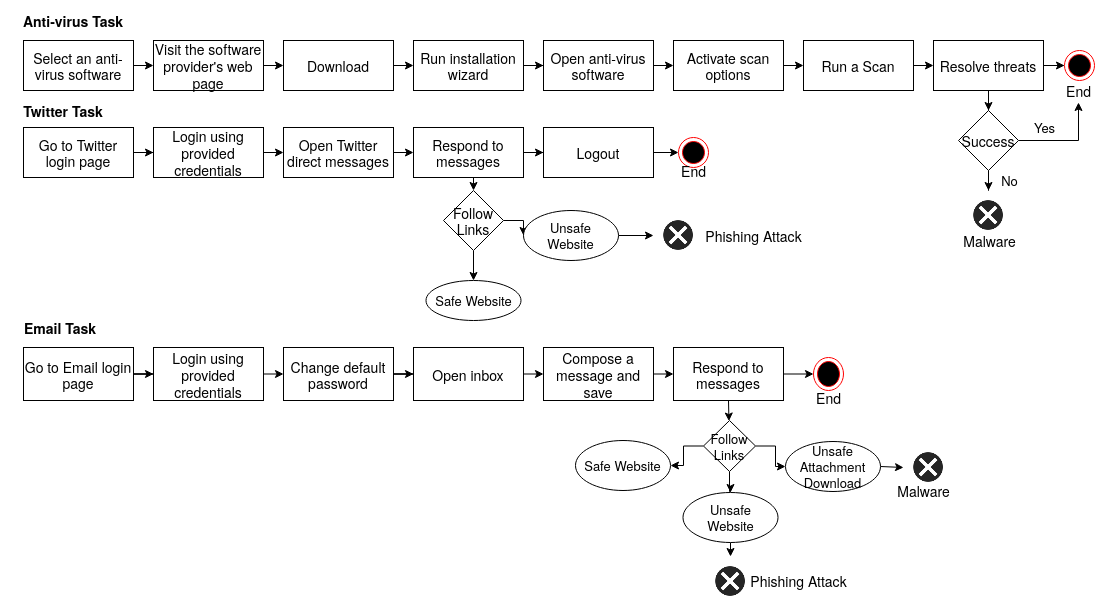
\includegraphics[width=1.1\columnwidth, keepaspectratio=true]{img/tasks.png}
  \caption{Sandbox task breakdown}
  \label{fig:tasks}
\end{figure}

The anti-virus task consisted of three sub-tasks: (1) given a legitimate and an illegitimate antivirus software, the user was asked to choose one (choice), (2) install the selected software and configure it to be used in the computer (install) and (3) run the software on the computer and remove threats (scan). In the post-survey, question 4 measures self-efficacy of the choice, question 9 measures the self-efficacy of the install and question 6 measures the self-efficacy of the scan. From the 62 participants only 11 completed all three sub-tasks, while 32 participants skipped the anti-virus task altogether. Those who did not complete the task skipped the install or scan or both. All 11 participants who completed all three sub-tasks installed the legitimate anti-virus software. This shows that users who practice computer security typically execute similar actions when they are placed in similar situations.

Table \ref{tab:avefficacy} shows the result of the two-tailed T-test that compares the self-reported efficacy between those who completed the choice task and those who did not is significant (P > 0.05). The same can be observed for the scan activity. However, the self-reported efficacy is not significant for the install task. This shows that for certain tasks that involve anti-virus software usage, users can incorrectly assess their self-efficacy when practicing computer security in self-reports.

\begin{table}[ht]
\begin{tabular}{|l|l|l|l|}
\hline
Activity & \begin{tabular}[c]{@{}l@{}}Completed \\ Efficacy Mean (SD)\end{tabular} & \begin{tabular}[c]{@{}l@{}}Incomplete \\ Efficacy Mean (SD)\end{tabular} & P \\ \hline
Choice  & 4.181 (0.603) & 2.944 (0.998) & 0.00096 \\
Install & 3.6 (1.055)   & 3.428 (0.851) & 0.636   \\
Scan    & 4.0 (0.707)   & 2.875 (1.147) & 0.005   \\ \hline
\end{tabular}
\caption{Self reported self-efficacy differences between those who completed all anti-virus sub-tasks and those who did not complete the task.}
\label{tab:avefficacy}
\end{table}

Our post survey contained 3 questions (questions 14 - 16), which evaluated self efficacy of communicating safely on Twitter. As seen in Figure \ref{fig:tasks} the Twitter task contained the least number of steps. Furthermore, the action ``Respond to messages'' is a repetitive action. The action makes the user to read and respond to the three messages in their Twitter inbox. All 61 participants who completed the task opened/responded to at least one of the three messages.

\begin{table}[ht]
\begin{tabular}{|l|l|l|l|}
\hline
Question &
  \begin{tabular}[c]{@{}l@{}}Mean (SD)\\ Visited phishing \\ link\end{tabular} &
  \begin{tabular}[c]{@{}l@{}}Mean (SD)\\ Did not visit\\ phishing link\end{tabular} &
  P \\ \hline
14 & 4.31 (0.87) & 4.04 (0.85) & 0.298 \\
15 & 4.13 (1.20) & 3.93 (0.96) & 0.571 \\
16 & 4.31 (0.87) & 3.84 (0.85) & 0.075 \\ \hline
\end{tabular}
\caption{Self reported self-efficacy means (standard deviation in parenthesis) between those who visited the phishing link and did not visit the phishing link during the Twitter task}
\label{tab:twitvisitedphishing}
\end{table}
Table \ref{tab:twitvisitedphishing} shows the result of the two-tailed T-test that compares the self-reported efficacy between those who visited the phishing web page following the link that appeared on their Twitter direct message and those who did not. We compute separate p-values for each question that asks the user to rate their self-efficacy. It can be seen that the participants evaluated their self efficacy to recognize phishing attempts while communicating on Twitter higher than it actually was. There is no significant difference between the self-efficacy ratings participants who clicked the phishing link and the participants who did not, P > 0.05 for all questions.

\begin{table}[ht]
\begin{tabular}{|l|l|l|l|}
\hline
Question & \begin{tabular}[c]{@{}l@{}}Mean (SD)\\ Visited-No Passwd\end{tabular} & \begin{tabular}[c]{@{}l@{}}Mean (SD)\\ Visited-Yes Passwd\end{tabular} & P \\ \hline
14 & 4.25 (0.9) & 4.02 (0.85) & 0.335 \\
15 & 4.25 (0.9) & 3.90 (0.97) & 0.316 \\
16 & 4.25 (0.9) & 3.80 (0.84) & 0.305 \\ \hline
\end{tabular}
\caption{Self reported self-efficacy means (standard deviation in parenthesis) between those who visited the phishing site and did not submit their passwords and those who visited the site and submitted their passwords. P value is the two-tailed T-test}
\label{tab:twitvisitedphishingpass}
\end{table}

A similar observation can be made for the situation where the participant visited the phishing site and submitted their password information. Table \ref{tab:twitvisitedphishingpass} shows that although there is no statistically significant difference between self reported self-efficacy ratings for the participants who visited the phishing site and also submitted their password and those visited the site but did not submit the password, those who submitted the password further compromised their security. 

Users found it difficult to correctly assess their self-efficacy in practicing caution when communicating with email. Questions 21 and 22 in the post-survey asked users to rate their self efficacy. When encountered with an email containing a phishing link, two tailed T-test showed that there is no statistical significance between self-efficacy ratings given by users who did not follow the phishing link against the users who did (P > 0.05). All users, who visited the phishing link, except one submitted their login credentials to the phishing web site. The users who submitted their login credentials had a mean self-efficacy rating 3.89 (SD=0.90). Similar observation can be made from users who downloaded malicious attachments that come with email. Two tailed T-test revealed that there is no statistical significance (P > 0.05) between the self-efficacy ratings given by users who downloaded malicious attachments  from email against the users who did not.

We focus on cues that are available on the computer system to evaluate how cues-to-action affect the user's computer security behavior. For the anti-virus usage task, we focused on two cues: (1) whether or not the download page was secure (has HTTPS with SSL lock icon), and (2) software provider/web page appears to be legitimate (look and feel, content etc.). Secure download was tested with post-survey question 29 and legitimate provider cue was tested with post-survey question 8. The Twitter task cues were tested with questions 17, 18, 19, 26. We considered cues such as: (1) unknown sender, (2) suspicious message content, (3)shortened URL links that appear in twitter messages and (4) secure HTTPS Twitter login page. For the email task we used two cues: (1) secure HTTPS web pages and (2) Firefox expired certificate warning. The post-survey questions 20 and 28 evaluated whether or not users picked up on these cues for email.

In the anti-virus task, we used user responses to question 8 to compare self-reports of ability to recognize safety of anti-virus software by looking at the provider's web page. Participants' mean self-report value was 3.86 (SD=0.94) for the safe software and 3.00 (SD=1.00) for the unsafe software. Two tailed, T-test between the users who selected the safe software vs. the unsafe software showed that the mean difference is significant (P < 0.05). This allows us to conclude that the web page content cue helps users to select a safe anti-virus software. Question 29 had categorical responses. We used the Chi-square test of independence to determine whether the HTTPS cue is associated with users selecting a safe software. Results showed we can reject the null hypothesis that the HTTPS cue is not associated with users selecting safe software (P=0.002, df=2).

In the Twitter task question 17 evaluated the unknown sender cue. Question 18 evaluated the shortened URL links in the message cue. Question 19 evaluated the suspicious message content cue. Question 26 evaluated the HTTPS with SSL padlock icon cue. Two tailed T-test for ability to recognize cues for questions 17, 18 and 19 between participants who visited the phishing link and participants who did not were not significant (P > 0.05). Question 26 contained categorical responses. We used the Chi-square test of independence to determine whether the HTTPS cues is associated with user with users following unsafe links on Twitter. Results showed we can not reject the null hypothesis that the HTTPS cue is not associated with users following unsafe links on Twitter (P=0.84, df=2).

In the email task question 20 evaluated the cue of the expired certificate warning generated by the browser when following a link. Question 28 evaluated the HTTPS cue, when submitting personal information to web sites. Two tailed T-test for ability to recognize cues for questions 20 between participants who followed a link to visit an unsafe website and those who did not was not significant. Participants' mean self-report value was 3.47 (SD=0.77) for those who visited the unsafe site and 3.82 (SD=0.88) for those who did not visit the unsafe site. Question 28 contained categorical responses. We used the Chi-square test of independence to determine whether the HTTPS cues is associated with user with users submitting personal information to web sites. Results showed we can not reject the null hypothesis that the HTTPS cue is not associated with users submitting personal information to websites (P=0.85, df=2).


\section{Discussion}
The results of our study validate the conclusions in previous studies, which states that human users' security related behavior often does not match their stated intentions \cite{davinson2010, govani2005, national2010}. 
For the software installation tasks, the Twitter task and the email task, the participants overestimated their efficacy to recognize undesirable consequences. This shows that the home computer users do not think about the post conditions of the actions they execute in the computer and therefore can benefit from an intervention system that help them identify actions leading to undesirable consequences.
Furthermore, the cues-to-action we have discussed in this study are preconditions that exist in the computer system. For example, identifying whether the web page the user is visiting contains the HTTPS SSL padlock icon, or whether the user is opening an email sent by an unknown (not in address book) sender. Although we expected users to recognize the preconditions (cues) leading to undesirable consequences all the time, this study concludes that it is not the case. We found that the users can recognize certain preconditions that exist in the system (e.g., the web page that they are visiting to download a software is secure) to help them avoid undesirable consequences. However, in other situations they miss these cues (e.g., recognizing unsafe web pages on Twitter) and as a result may end up compromising security.
Therefore, the design of software to assist home computer users in avoiding security and privacy vulnerabilities should be motivated by careful studies of their behavior and perceptions.

PsychoRithm sandbox environment allowed us to place human users in simulated scenarios that compromised their security/privacy and record their actual responses and at the same time capture the self-reported data on how users perceive their confidence in identifying risky situations (self-efficacy) and recognize cues that indicate danger (cues-to-action). Although, we are measuring factors that affect the computer security behavior of users (extracted from the Health Belief Model), our objective in this study is not to validate the model, but rather highlight that regardless the perceived self-efficacy and availability of cues, human users can still end up compromising their security. 
When the threat is immediate, if the user is not interrupted they may end up putting their safety in even more risk. 
To this end, the intervention models presented in this dissertation target helping human users avoid undesirable consequences.

In this study we mainly looked at three common home computer user tasks:
\begin{itemize}
\item Using anti-virus software to secure the computer
\item Communicating with Twitter direct messages
\item Using email
\end{itemize}

By analyzing the results, we identified important conditions that should be addressed when designing an intervention system to help human users. First, even though users were given step-by-step instructions for completing these tasks, they rarely follow the script. 
The users repeated the same action multiple times, while some actions were omitted altogether. 
The implication of this observation is that intervention systems that monitor users to help them avoid unsafe consequences need to handle noisy and/or missing actions in the observations.
Furthermore, any partially complete task (i.e., a sequence of actions) that has been safe upto now may quickly turn unsafe. 
This means that the intervention decisions need to be made online. 
Users perform a large number of actions; while few of them incur much risk, some are pivotal in triggering vulnerabilities. For example, from our using email task, opening email action itself is not a risky action. 
However, when the email is from an unknown sender and contains suspicious attachments, preconditions to a malware vulnerability have manifested within the system. In this state, the opening email, although a normal action for a human user, is actually high risk action.
This means that intervention models need to search for multiple ways for accomplishing the same task. Modeling the problem as a state/action transition system using automated planning allows us to accomplish this requirement. When the problem is modeled as a planning domain, automated planners can be used to generate diverse plans, to sample the space of possible plans that can lead to one or more vulnerabilities and help
estimate the probability that particular actions lead to triggering the vulnerabilities.


Second, the objective of the intervention system will be to identify when a user's action(s) may be complicit in triggering the threats and help the user avoid the undesirable state (security or privacy breach).
Given a fine-grained model of user and attacker actions and states of the system as an automated planning domain, the intervention system should be able to identify actions that can lead to triggering a vulnerability.
A previous study \cite{byrne2016} showed that users pay more attention to the benefits of the activities than the risk; they have goals that they want/need to achieve and are willing to take the risk to achieve them. 
Many triggering actions may be normal activities (e.g., reading email, clicking on links)
with the user more focused on the goal than on the risk.
Thus, the undesirable consequence recognition problem needs to take into account the user's intention as well as the undesirable consequence.
Undesirable consequences prediction is assessing whether an action is likely to lead to undesirable consequences, immediately or as part of an action sequence, or may provide conditions
that an attacker can exploit. 
User intentions recognition determines what the user is intending to do through his/her actions, the short or long term goals.
The intervention decision involves a trade-off in early recognition of potential danger of an action versus the certainty that the effects will occur. In the chapters that follow we examine how different metrics captured from the planning problem representation can be used to assess that trade-off.
To help the user trade-off benefits versus risks, we also need to know what the user thinks he/she
is trying to accomplish. In some cases the goal may be explicitly stated in terms of actions and post-conditions. In other cases, the user's goal may be unknown. We consider both these conditions in the intervention models we present.


Third, personalization becomes most important when the intervention system must decide how to prevent an imminent security/privacy threat or decide what to do when one has been detected. Simply preventing a user from doing something they want to do will undoubtedly result in the security software being disabled. 
Our underlying hypothesis is that security will be more effective when the user is a partner with the system in the security interventions. In Chapter 6 of this dissertation, we present an intervention model designed for human users that uses automated planning to guide the user away from the undesirable consequence by giving hints.



\section{Concluding Remarks}
The design of software to assist home computer users in avoiding security and privacy vulnerabilities should be motivated by careful studies of their behavior and perceptions.
In this work, we created sandbox software to simulate, in a protected environment,
the user interface to an operating system and browser so that we could capture subject actions related to security and privacy in a realistic setting. 
Each subject took an initial survey to assess demographics, computer self-efficacy and perceptions of security/privacy, then used the simulator to ``setup and test basic functionality in a recently purchased computer'' (the cover story) and then took a survey to assess their perceptions of what they had done. 
In our analysis, we found that the users (adults taking a psychology course in Colorado State University) are unaware when they have made poor decisions and have triggered vulnerabilities. 
In the following chapters we present intervention models designed to automatically detect when such situations occur, i.e., that a user’s action(s) may be contributing to triggering a security or privacy threat.
To identify pivotal events, the appropriate system states and user actions must be monitored and compared to a model of actions that can lead to triggering a vulnerability.
We use automated planning to model the actions in environments where the user's decision making context differs in terms of what the user knows about the domain and the type of observational data available to identify pivotal events.

If an action that contributes to a trigger is suspected, it should be put in the context of what the user is trying to do and an estimate of how likely the action is to actually trigger the vulnerability.
Therefore, future studies for developing tools to help human users practice cyber-security must employ surveys, sandbox simulations and lightweight in situ monitoring to accurately understand the human users' decision making context. 
While the sandbox offers a controlled environment, in situ affords realism and the ability to conduct longitudinal studies. Therefore, lightweight tools need to be developed for unobtrusively monitoring the user and logging actions related to security. Longitudinal evaluation of intervention techniques is important to determine whether the new techniques will eventually be susceptible to
habituation (a major issue with current intervention techniques) and to examine if user’s actions change over time as security awareness increases.

In this study, we only analyzed two specific user traits: self-efficacy, and cues to action when we presented the user with choices of anti-virus software to install and asked them to do ordinary tasks like reading/sending email and reading/responding to tweets.
Future studies need to extend the state/action model of the home computer environment by including more scenarios and attacker actions.
Although self-efficacy and cues to action capture important aspects of the user's decision making context in the home computing environment: post-conditions and pre-conditions of actions the user executes respectively, there are many other factors that can define the decision making context of a human user (e.g., computer experience, decision-making psychometrics, risk aversion, perceived social status, the need
to belong). Developing realistic scenarios that capture these additional traits to study human user behavior in security situations is a challenging yet critical step in developing more personalizable intervention models.





\chapter{Intervention by Recognizing Actions That Enable Multiple Undesirable Consequences}
\label{chap:ch4}
In this chapter, we discuss the first intervention model for an observer who intervenes to help the user avoid multiple undesirable consequences.
The dimensions of the Intervention Problem presented in this chapter are summarized in Table~\ref{tab:dim2}.

\begin{table}[ptb]
\caption{Dimensions of the Critical Action Recognition Problem}
\label{tab:dim2}
\begin{tabular}{|l|l|}
\hline
\textbf{Dimension} & \textbf{Domain Specific Properties} \\ \hline
Actors in the environment & User, Attacker, Observer \\ \hline
Goals hidden to the observer & \begin{tabular}[c]{@{}l@{}}User's goal is hidden\\ Multiple known undesirable states\end{tabular} \\ \hline
Types of observations & \begin{tabular}[c]{@{}l@{}}The observer observes the user's actions\\ The observer only observes the effects of the attacker's actions\end{tabular} \\ \hline
Noise in observations & Has missing and extraneous observations \\ \hline
Intervention recovery & Block the recognized undesirable action \\ \hline
\end{tabular}
\end{table}

In Chapter~\ref{chap:ch3}, we showed that many security threats such as software downloads and phishing require user action or at least acquiescence. 
The threats are triggered because the user did not understand the consequences of reaching the undesirable state or was not aware of the undesirable state from the start.
The implication of this finding is that the observer needs to recognize on time that the plan the user is following will have an undesirable consequence.
In Chapter~\ref{chap:ch2}, we discussed Plan Recognition as the problem of inferring the goal(s) of an actor by constructing a plan from a sequence of actions or observations.
To recognize actions that may lead to undesirable consequences, we propose a variant on plan recognition, where the undesirable consequences prediction problem is viewed as a form of reverse planning; it leverages plan graphs from an existing planner to project possible undesirable outcomes and then trace back to actions critical to their occurrence.
We formulate the Undesirable Consequence Recognition problem as a planning problem of three domain independent, weighted metrics: \textbf{timeliness}, \textbf{certainty} and \textbf{desirability}. 
Against an ideal baseline, we examine the trade-offs in choosing the correct intervention point by varying the weights associated with the metrics, the observability and the noise in observations.

\section{Background}
A wealth of literature in plan and goal recognition has examined how to infer a single agent's plan \cite{GeibGoldman09, ramirez2009plan}, the agent's goal \cite{ramirez2011goalrecog, yin2004high}, or the goals or plans of multiple agents \cite{banerjee2010mpr, kaminka2002monitoring}. Recent work has even examined plan/goal recognition in the face of noisy observations \cite{geib2005partial, vattam2015case} or extraneous actions \cite{gal2012plan, sohrabi2016finding}. 
Yet relatively little of this research considers the question of when to intervene if one wants to thwart the plan or goal, for example, if the agent we want to disrupt is at the risk of producing an undesirable state. 
The decision of when to intervene must be made judicially. 
Intervening too early may lead to wasted effort chasing down false positives, helpful warnings being ignored as a nuisances, or leaking information for the next attack. 
On the other hand, intervening too late may result in undesirable consequences.

Our motivating application is a software agent that monitors the state of a personal computer to help home computer users avoid security and privacy vulnerabilities. 
Home computer users are viewed as the ``weakest link'' in computer security because they lack the time, knowledge and resources to defend against the increasing incidents of computer security and privacy threats \cite{sasse2001transforming}. 
Moreover, some threats, such as software downloads and phishing, require user action or at least acquiescence \cite{howe2012psychology}. Security analysis for home computer users focuses on identifying threats on a personal computer by modeling attacker actions, the system state of the computer and computer user's actions, including both ordinary and risky actions. 
The Personalized Attack Graph (PAG) extends the attack graph model \cite{Sheyner2002} to support individual computer/user level granularity and by representing the states and actions in PDDL \cite{urbanska2013}. 
Attacker actions do not include actions that cannot be observed on the home computer. System states can include levels of partial compromise (e.g., access to the password key-chain), configuration information (e.g., operating system), and state changes achieved on specific system components (e.g., implanting a keystroke logger).

In this work, we examine how well an algorithm can determine the best intervention point for the cyber-security application, calling it a ``\textit{critical trigger action}'' because it may lead to an undesirable state. 
As each situation may have a unique definition of the ideal intervention point, we formulate intervention as a combination of three domain independent metrics: (1) \textbf{timeliness}, which quantifies how soon the undesirable state may occur, (2) \textbf{certainty}, which highlights frequently occurring actions as important, and (3) \textbf{desirability}, which measures the contribution of the action to user's own objective. The desirability metric helps separate common harmless actions that further the user's actual goal from harmful actions to be avoided. A critical trigger action is a user action that maximizes the linear combination of these three metrics.

Given a PDDL domain model, a set of undesirable states to avoid, and an observation trace of actions, our algorithm identifies critical trigger actions. An intervention is correct if, compared to a ground truth trace, the algorithm (1) ignores extraneous actions (i.e., as true-negatives) and, (2)
identifies actions leading to undesirable state (i.e., as true-positives). We begin with a study of traces taken from a human subject study for computer security. We then generalize our results to four benchmark planning domains and
consider the impact of missing and extraneous observations of actions and test the algorithm. Across all benchmark domains, certainty and desirability metrics perform well in ignoring extraneous actions, while the timeliness metric and
it's combinations with certainty and desirability perform well in identifying true positives. Thus, in this work we have identified two metrics that are sensitive to noise in action based observation traces and a metric that is sensitive to partial observability of actions.



\section{Intervention in Cyber-security Domain}
Before introducing a formal definition, we present an example to clarify the key concepts. 
Suppose a user wants to  achieve the goal $G$ (e.g., \texttt{read email}) but there exists an undesirable state $U$ (e.g., \texttt{installation of malicious software}). 
Figure~\ref{fig:cybersecproblem} illustrates the \emph{possible} manifestation of $U$. 
The user has executed actions $a_1, a_2, a_3$ (e.g., \texttt{start email application, enter username/password, open inbox}) from the initial state $S_0$ in order to achieve  $G$.
Actions $a_1$, $a_2$, $a_3$ have resulted in the post conditions $S_{1}, S_{2}, S_3$ respectively. 
An intervening agent is observing the actions executed by the user and must intervene upon recognizing that the user has executed an action that will lead to $U$.

In order to intervene, the intervening agent considers possible plans that lead to $U$.
We denote a plan as a sequence of actions  followed in brackets by the undesirable state that results $(a_i, a_j, \ldots, [U])$.
We will call these \emph{undesirable plans} identified as $\Pi_U$ and denote a plan in the set as $\pi_{U}$.
Ideally, the user would continue toward achieving $G$ and not execute plans in $\Pi_U$.
However, by mistake or undue influence, the user may deviate from pursuing $G$ and unwittingly follow paths in $\Pi_U$. 
In the example in Figure~\ref{fig:cybersecproblem}, the intervening agent has observed the action sequence $O$ = $\{a_1, a_2, a_3\}$ the user has executed. 
In state $S_{3}$, the user may reach $U$ through a set of undesirable plans $\Pi_{U}=\{(a_5, a_8, a_7[U]), (a_5, a_8, a_6, a_{14}[U]), (a_{4}, a_{10}[U]), (a_4, a_9, a_{16}[U]), (a_4, a_9, a_{12}, a_{11}, a_{13}[U]),\\ (a_4, a_9, a_{11}, a_{12}, a_{15}, a_{16}[U]), (a_{12}, a_{13}[U]), (a_{12}, a_{15}, a_{16}[U]), (a_{12}, a_{15}, a_{11}, a_{12}, a_{13}[U]), \\ (a_{12}, a_{15}, a_{11}, a_{12}, a_{15}, a_{16}[U])\}$.
The actions in the plans in $\Pi_U$ are the \textbf{candidate trigger actions}.
A candidate trigger action is an action that appears in at least one plan in $\Pi_U$.
The intervening agent's question is: \textit{given the current state $S_{3}$, which action in the set of candidate trigger actions is the best action to intervene if observed?}

\begin{figure}[tpb]\centering{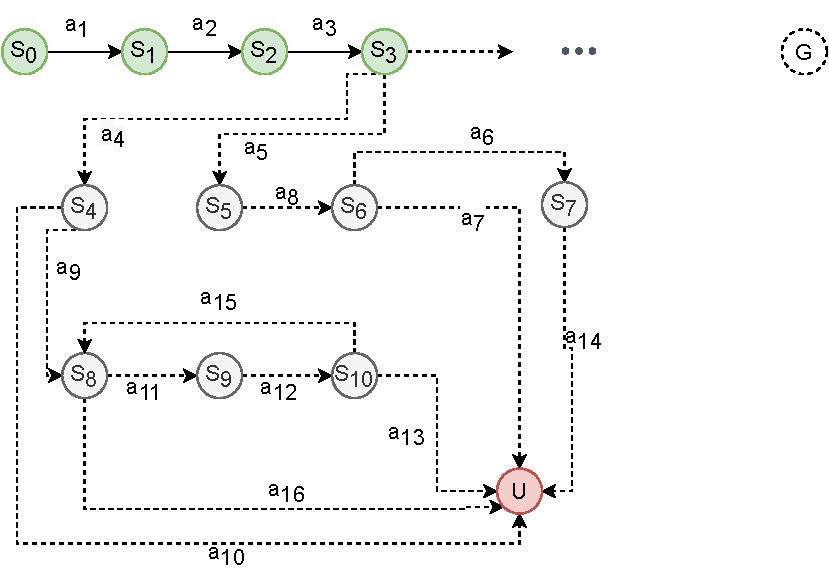
\includegraphics[width=0.8\columnwidth]{img/undesirable.pdf}}
	\caption{An application domain where a user executes the actions $a_1, a_2, a_3 $ to transform initial state $S_0$ to a goal state $G$. An undesirable state $U$ may develop from state $S_{3}$ after $a_3$ has been executed, following the plans ($\Pi_U$) indicated by the dotted paths towards $U$.}
\label{fig:cybersecproblem}
\end{figure}

\subsection{The Intervention Problem: Recognizing Undesirable Consequences}
Given a domain $\mathcal{D}$ and a planning problem $P$, an automated planner generates the planning task $\Pi=\langle \mathcal{F}, \mathcal{A}, I, G\rangle$, where $\mathcal{F}$ is a finite set of grounded propositions, $\mathcal{A}$ is the finite set of grounded actions instantiated from the operator schemata $Op$, $I$ is the grounded propositions specifying the initial state and $G$ is the grounded goal specification. Objects in $\mathcal{O}$ are used to ground $\mathcal{F}$, $\mathcal{A}$, $I$ and $G$. Grounding replaces the variable terms in the parameter lists of the propositions, action schema, goal specifications with constant/non-constant objects. 

We defined a domain model for the cyber-security domain using PDDL (Planning Domain Definition Language) a generalization of STRIPS, shown in Figure \ref{fig:cybersecdomain}. In total this domain model has 45 actions, 47 types, 70 constants and 55 predicates.
This STRIPS domain model captures the home computer user cyber-security scenarios simulated in the Psychorithm sandbox environment described in Chapter~\ref{chap:ch3}.

\begin{figure}[pbt]
\noindent\fbox{
 \parbox{\textwidth}{\raggedright: 
{\small
\texttt{(define (domain attackgraph-typed)}\\
\texttt{\hspace*{35pt}(:requirements :strips :adl :equality :typing \hspace*{35pt} :disjunctive-preconditions)}\\
        \hspace*{35pt}\texttt{(:types unknown software misc - object)\\
       \hspace*{35pt} \texttt{account certificate email-ID file key site user attacker vulnerability-type password direct-message device database parameter permission process username response request - misc}\\
\hspace*{35pt} \texttt{browser editor webmailer plug-in site-creating-software server-connecting-software server anti-virus OS desktop-app server-app malicious-software - software}\\
\hspace*{35pt} \texttt{phishing-site server-site normal-site - site}\\
\hspace*{35pt} \texttt{phishing-site-email phishing-site-twitter - phishing-site}\\
\hspace*{35pt} \texttt{attacker-remote attacker-local - attacker)}
        }\\ [15 pt]
\hspace*{35pt}\texttt{(:constants \\ 
\hspace*{35pt}user1-email-account user1-twitter-account - account \\
\hspace*{35pt}pc-doctor security-shield - anti-virus \\
\hspace*{35pt}browser-firefox - browser \\        \hspace*{35pt}phishing-direct-message - direct-message \\
\hspace*{35pt}email-with-malicious-attachment - email-ID\\
\hspace*{35pt}squirrelmail - webmailer\\
\hspace*{35pt}user1-twitter-password - password $\ldots$ )\\[15 pt]
}
\hspace*{35pt}\texttt{(:predicates \\
\hspace*{35pt}(information-available ?aUser - User ?anAccount - account) \\
\hspace*{35pt}(user-has-email-account ?anAccount - account)\\
\hspace*{35pt}(direct-message-received ?dmsg - direct-message)\\
\hspace*{35pt}(anti-virus-software-selected ?av - anti-virus) \\
\hspace*{35pt}(information-leakage ?anAccount - account $\ldots$ )\\[15pt]
}

\hspace*{35pt}(\texttt{:action user-visit-antivirus-download-site}\\
\hspace*{35pt}\texttt{:parameters (?U - user ?aBrowser - browser ?aSite - site \\\hspace*{35pt} ?av - anti-virus)}\\
\hspace*{35pt}\texttt{:precondition ( and (logged-onto-system ?U) \\\hspace*{35pt} (use-software ?aBrowser) (running ?aBrowser) \\\hspace*{35pt} (= ?aSite antivirus-software-download-site) \\\hspace*{35pt} (not (installed ?av))  (not (running ?av)) )}\\
\hspace*{35pt}\texttt{:effect (and (user-visits-site ?U ?aSite))}
)\\[15pt]

\hspace*{35pt}\texttt{(:action user-opens-attachment-through-webmail}\\
\hspace*{35pt}\texttt{:parameters (?U - user ?aBrowser - browser ?WM - webmailer \\\hspace*{35pt}?aSite - site  ?anAccount - account ?Msg - email-ID  ?F - file )}
\hspace*{35pt}\texttt{:precondition (and  (use-software ?aBrowser) (running ?aBrowser) \\\hspace*{35pt}(user-visits-site ?U ?aSite) (= ?aSite webmail-site)\\\hspace*{35pt}(user-has-email-account ?anAccount)\\\hspace*{35pt}(= ?anAccount user1-email-account) (msg-opened ?Msg)\\\hspace*{35pt}(mail-attachment ?Msg ?F) (logged-onto-system ?U))}\\
\hspace*{35pt}\texttt{:effect (opened ?F))} 
 )\\\hspace*{35pt}$\ldots\ldots$
}
}
}
\caption{The cyber-security PDDL domain model snippet}
\label{fig:cybersecdomain}
\end{figure}

\sloppy
\begin{definition}
An observation trace $O$ is a sequence of observed actions $O = \{o_1, o_2, ... ,o_n\}  \;where\; o_i\in \mathcal{A}\; and \; i=1,2, \dots ,n\; (n = $ length of observation trace) and states resulting from execution of actions $o_i\in O$ are known. 
\end{definition}

Traces may contain extraneous or missing actions.  An \emph{extraneous action} is an observation $o \in O$ such that the state resulting from executing $o$ is never added to the state (i.e., set of state variable predicates that are true) by any of the actions $a_i \in \pi_U$. A \emph{missing observation} with respect to $\pi_U$ occurs when the state resulting from executing $o$ is added to the global state by an of the actions $a_i \in \pi_U$, and $o \notin O$.

When we are looking for possible paths leading to an undesirable state, we search for a \textbf{undesirable plan} $\pi_U = \{a_1, \dots ,a_k\}$ of length $k$ that entails one or more undesirable states $U\subseteq \mathcal{F}$ and $a_i \in A$. There may be more than one undesirable plan, in which case we consider a set of undesirable plans $\Pi_U$. In the example in Figure \ref{fig:cybersecproblem}, the domain has only one undesirable state $U=\lbrace U_1\rbrace$.


\begin{definition}
An intervention problem $T = \langle \mathcal{D}, O, I, U \rangle$ consists of a planning domain $D$, a sequence of observed actions  $O \subseteq \mathcal{A}$, an initial state $I \subseteq \mathcal{F}$, a set of undesirable states $U\subseteq \mathcal{F}$.
\end{definition}
The solution to the intervention problem is a binary decision for each action in the observation trace, $o \in O;  o \rightarrow \lbrace Yes, No \rbrace$ indicating whether it was identified as a critical trigger action ($Yes$) or not ($No$).


\subsection{Identifying Critical Trigger Actions}
A \textbf{critical trigger action} $c_i$ is a  action at $o_i \in O, i\leq |O|$ that maximizes the metric function $V (c_i)$, which we define now.

We recognize two forms of candidate trigger actions in the observation trace: strong and weak. 
A strong trigger can actively contribute to causing the state (e.g., as an effect or by satisfying a required precondition) or allow another actor to cause it. 
A trigger may also weakly contribute to the causation of the undesirable state(s) and may not be worth intervening to prevent. 
Consequently, we add a layer to the intervention problem to support application specific ranking about which actions are most ``critical'', i.e., helpful in preventing the undesirable state(s). 
The key addition is an objective function that allows a tunable combination of metrics.

Our focus is on identifying the intervention point as early as  \textit{helpful} when a user may be triggering an undesirable state. 
The concept of helpful is similar to the value of alerts described in \cite{Wilkins2003} which recognized that it is important to be judicious in interrupting a user in scenarios where humans and machine agents interact with each other: ``don't ignore but don't annoy''. 
To this end, we start by defining a function composed of three  metrics to quantify the notion of helpfulness: \textbf{certainty}, \textbf{timeliness} and \textbf{desirability}. 
These metrics are calculated based on a set $\Pi_U$.


When producing the set of alternative undesirable plans $\Pi_U$, as representative of a set of possible trajectories toward an undesirable goal, it would be best to consider alternatives that are non-obvious and diverse from each other rather than just the optimal plan.  
This is especially important in long-running processes with complex traces or when a sub optimal plan contains a longer, but perhaps more easy to trigger, path to the undesirable state.

{\it Certainty} measures the likelihood of action $a$ occurring in $\Pi_U$.
\begin{equation}
\label{eq:certainty}
Certainty (a|\Pi_U)  = \frac{|\pi_U \in \Pi_U \textup{ in which}\; a\; \textup{occurs}|}{|\Pi_U|}
\end{equation}
Actions occurring frequently in $\Pi_U$ indicate the importance of that action toward causing $U$. For example, if an action $a$ occurs in all plans $\Pi_U$, the certainty metric will assign a high value to $a$, giving it a higher probability of being selected as a critical trigger compared to a less frequent action. 

{\it Timeliness} requires knowing what actions could yet be observed, which might effect the causation of the undesirable state. 
For this study, timeliness is measured by the maximum normalized steps remaining in $\Pi_U$ in which the action a occurs. 
Timeliness quantifies how soon an observation will trigger the undesirable state. 
Therefore, we compute the maximum in discrete time as opposed to the minimum because it indicate that an undesirable state is developing but not imminent and allows time to recover. 
Let $n$ be the remaining number of steps in $\pi_U \in \Pi_U$ after some action $a$. Then,
\begin{equation}
\label{eq:timeliness}
Timeliness (a|\Pi_U) = \max_{\pi_U \in \Pi_U}\left(\frac{
	\max\left( n \right)\
	}{\; |\pi_U|}\right) 
\end{equation}

{\it Desirability} measures the effect of an action on user's goals, which is ignored in the other two metrics. 
In the Intervention by Undesirable Consequence Recognition problem the intervening agent is only aware of the undesirable state the user wants to avoid.
Although the user's goal is hidden to the intervening agent, the intervention decision must also consider how the candidate trigger actions contribute toward the user's goal to allow some freedom for the user.
In Chapter~\ref{chap:ch3}, we showed that in the cyber-security domain, most actions users execute to accomplish a goal are harmless actions while only a few of them put the user at risk.
We capture this property with the Desirability metric and separate common harmless actions (e.g., user opening web browser) from avoidable ones and connects the observations to knowledge of the user's goals.
If an action appears often in the candidate trigger actions then that action is a common, harmless action and more desirable.
In contrast, actions that appear less often in the candidate trigger actions are comparatively more undesirable.
The intervening agent must consider the undesirable actions with higher priority.
Consequently we downgrade the contribution of the desirable actions to criticality by defining Desirability as a negative metric.
\begin{equation}
\label{eq:desirability}
Desirability (a|\Pi_U) = - \left( \frac{|\textup{appearance of}\; a\; \textup{ in } \Pi_U|}{\sum_{i=1}^{|\Pi_U|}\left | \pi_i \right |} \right)
\end{equation}
Together, these metrics define the function $V(a)$ for candidate trigger action $a$ for a weighting provided by $\alpha$, where $\alpha$ $=\lbrack\alpha_1, \ldots, \alpha_m \rbrack$, $\alpha_i$ is in the range $\lbrack0,1\rbrack$, $m$ is the number of objectives and $\sum_{1}^{m}\alpha_i = 1$:
\begin{equation}
\label{eq:function}
V(a) = (\alpha_1 \times Certainty (a|\Pi_U)) + (\alpha_2 \times Timeliness (a|\Pi_U)) + (\alpha_3 \times Desirability (a|\Pi_U))
\end{equation}

Table \ref{tab:metrics}, shows how the critical trigger action is identified using the proposed objective function for the example in Figure \ref{fig:cybersecproblem} given the observation sequence of actions $O=\{a_1, a_2, a_3\}$. 
In state $S_{3}$, assuming equal weighting of metrics, the algorithm identifies $a_{12}$ to be the action that maximizes the objective function, and returns it as a possible point of intervention. 
Table \ref{tab:metrics} also shows how this decision is affected by the choice of $\alpha$. If only certainty metric is used ($\alpha=\lbrack1,0,0\rbrack$) action $f$ gets selected as the intervention point. 
Using only timeliness metric ($\alpha=\lbrack0,1,0\rbrack$) yields three possible intervention points: $a_{12}$, $a_5$ and $a_4$. 
Finally, using only desirability yields four possible intervention points: $a_{10}$, $a_6$, $a_7$ and $a_{14}$.

\begin{table}[tpb]
	\centering
		\caption{Certainty (C), timeliness (T), desirability (D) computations for each candidate trigger action for the example in Figure \ref{fig:cybersecproblem}. $V(a)$ is the value returned by the critical trigger multi-objective function assuming equal weighting ($\alpha=\lbrack0.33,0.33,0.33\rbrack$), only C ($\alpha=\lbrack1,0,0\rbrack$), only T ($\alpha=\lbrack0,1,0\rbrack$) and only D ($\alpha=\lbrack0,0,1\rbrack$) for each candidate trigger action.}
\label{tab:metrics}
	\resizebox{\textwidth}{!}{
		\begin{tabular}{|c|l|l|l|c|c|c|c|}
			\hline
			\multirow{2}{*}{} & \multicolumn{1}{c|}{\multirow{2}{*}{C}} & \multicolumn{1}{c|}{\multirow{2}{*}{T}} & \multicolumn{1}{c|}{\multirow{2}{*}{D}} & \multicolumn{1}{l|}{$\alpha$ = {[}0.33,0.33,0.33{]}} & \multicolumn{1}{l|}{$\alpha$ = {[}1,0,0{]}} & \multicolumn{1}{l|}{$\alpha$ = {[}0,1,0{]}} & \multicolumn{1}{l|}{$\alpha$ = {[}0,0,1{]}} \\ \cline{5-8} 
			& \multicolumn{1}{c|}{} & \multicolumn{1}{c|}{} & \multicolumn{1}{c|}{} & $V(a)$ &$V(a)$ & $V(a)$ & $V(a)$  \\ \hline
			$a_5$ & 2/10=0.2 & max(3/3,4/4)=1.0 & -2/39=0.05 & 0.38 & 0.2 & \textbf{1.0} & -0.05 \\
			$a_4$  & 4/10=0.4 & max(2/2,3/3,5/5,6/6)=1.0 & -4/39=0.1 & 0.43 & 0.4 & \textbf{1.0} & -0.1 \\
			$a_{11}$  & 4/10=0.4 & max(3/5,4/6,3/5,4/6)=0.6 & -4/39=0.1 & 0.30  & 0.4 & 0.6 & -0.1 \\
			$a_{12}$  & 6/10=0.6  & max(2/5,3/6,2/2,3/3,5/5,6/6)=1.0  & -6/39=0.15 & \textbf{0.48} & \textbf{0.6}  & \textbf{1.0} & -0.15  \\
			$a_8$ & 2/10=0.2 & max(2/3,3/4)=0.75  & -2/39=0.05 & 0.30 & 
			0.2  & 0.75 & -0.05   \\
			$a_{10}$ & 1/10=0.1   & max(1/2)=0.5   & -1/39=0.03 & 0.19   & 0.1  & 0.5  & \textbf{-0.03}   \\
			$a_9$ & 3/10=0.3   & max(2/3,4/5,5/6)=0.83   & -3/39=0.08 & 0.35   & 0.3  & 0.83 & -0.08   \\
			$a_{15}$ & 4/10=0.4   & max(2/6,2/3,4/5,5/6)=0.83  & -6/39=0.15 & 0.36   & 0.4  & 0.83 & -0.15   \\
			$a_{13}$ & 3/10=0.3   & max(1/5,1/2,1/5)=0.5    & -3/39=0.08 & 0.24   & 0.3  & 0.5  & -0.08   \\
			$a_6$ & 1/10=0.1   & max(2/4)=0.5   & -1/39=0.03 & 0.19   & 0.1  & 0.5  & \textbf{-0.03}   \\
			$a_7$ & 1/10=0.1   & max(1/3)=0.33  & -1/39=0.03 & 0.13   & 0.1  & 0.33 & \textbf{-0.03}   \\
			$a_{16}$ & 4/10=0.4   & max(1/3,1/6,1/3,1/6)=0.33  & -4/39=0.1  & 0.21   & 0.4  & 0.33 & -0.1 \\
			$a_{14}$ & 1/10=0.1   & max(1/4)=0.25  & -1/39=0.03 & 0.11   & 0.1  & 0.25 & \textbf{-0.03}  \\ \hline
		\end{tabular}
	}%
\end{table}

Intervention is different from the typical plan recognition problem because the intervening agent assumes that the user pursues some desirable goal but wants to also avoid any undesirable state. 
Furthermore, the intervening agent has no knowledge about the user's desirable goal and knows only the set of undesirable states the user should avoid. 
Our model views the user's attempt to achieve a desirable goal as a planning process. 
Plan recognition approaches that use plan library representation do not apply for the Intervention problem because they are focused on matching observed actions to prior plans to determine what goals the user is trying to achieve.
The problems with that are: (1) the observations may contain extraneous actions and (2) the plans that lead to the undesirable states may not encompass the user's goal (the user does not want to trigger the vulnerability, but rather to do something useful with his computer).
Therefore, the objective is to identify intervention points based on their potential to cause the undesirable state, while making sure that the actions are identified in an \textit{opportune time}.

 
Our intervention model borrows ideas from the generative plan recognition approaches and analyses the Planning Graph and operates incrementally.
This is similar to prior work by Sun et al. \citeyear{sun2007recognizing} and Hong \citeyear{hong2001goal}. 
Following work by Geib and Goldman \citeyear{GeibGoldman09}, we adopt a model focused on execution: what could be done next. 
In contrast to the works of Ramirez and Geffner \citeyear{ramirez2009plan,ramirez2010probabilistic} that assumed a fully observable state space, our approach takes into consideration the inherent unreliable nature of observations (missing and irrelevant actions) towards identifying critical trigger actions. 
Our solution employs PDDL and the Mosaic planner \cite{roberts2014} to sample possible plans from the current state. 
For each observation, the algorithm outputs whether or not it is a critical trigger action. 

\subsection{Undesirable State Recognition Algorithm}
Figure~\ref{fig:components} shows the seven-step decision cycle of the algorithm. As defined in the problem statement, the process takes as input: a PDDL domain, an initial state, a set of undesirable states and the objective function weights. 

\textbf{Step 1:} We assume the full observation trace is known in advance, with actions made available one at a time to identify the intervention point. However, the algorithm does not utilize information that can be gleaned from the full trace to yield the decision. Input to the algorithm in this step can also be replaced with application specific sensors.  

\textbf{Step 2:} For each possible undesirable state $U$, generate PDDL problem instances. In the first cycle, the initial state is from the input; in subsequent cycles, the state is updated in step 7. To extract applicable states for the next cycle, we chose to search forward the planning graph starting from initial state. This is because the unobservable actions require us to update state during search to accommodate those changes that are presupposed by the actions being able to execute. 

\textbf{Step 3:}
We opted to apply a diverse planner.  
A recent study examined the impact of diversity metrics in classical planning  \cite{roberts2014}, and a contribution from that work, the Mosaic planner, produces a set of diverse plans in a single run. 
A key finding by the authors of Mosaic was that existing diverse planners frequently produce plan sets containing actions not leading to the goal, which increased diversity but lacked justification for many applications. 
Mosiac returns $\Pi_U$ for $U$. 

Mosaic is built on top of the LAMA planner \cite{richterWestphal10.jair.LAMA}  with some patches applied to its parser from the current Fast Downward repository\footnote{See \smallurl{http://www.fast-downward.org/}}. It included three extensions to improve the plan set and produce diverse plans faster: the use of a tabu mechanism to guide search away from already known solutions, the use of multiple queues to increase the diversity of solutions explored, and the use of parsimony to bias the search toward goal-oriented solutions. From the family of variants, iterated Tabu A* (ITA) and Multi-queue A* (MQA), we use MQA-TS to compute up to 10 possible plans, based both on the recommendation of the authors and because it showed the most promise in prior work. 

\textbf{Step 4:} Extract unique actions in $\Pi_U$ as candidate trigger actions. Actions include the action name and the instantiated parameter values.

\textbf{Step 5:} Compute Certainty, Timeliness and Desirability for each candidate trigger action by iterating over the plans in $\Pi_U$, as defined in Function \ref{eq:function}. 

\textbf{Step 6:} Rank candidate actions by $V$. Flag the highest ranked actions as critical triggers corresponding to the current observation. Step 6 also evaluates the accuracy of the identified critical trigger by comparing against the observation. 
We use a ground-truth \textbf{u}ndesirable \textbf{p}lan (called UP) that achieves the undesirable state and assume that all actions in the ground-truth undesirable plan are critical triggers. 
If the algorithm returns the current observation as the critical trigger, then the decision is correct if the current observation is an action in the ground-truth undesirable plan (i.e., true-positive). 
Alternatively, if the current observation is not the critical trigger and it was also missing in the ground-truth undesirable plan (i.e., observation was an extraneous action and a true-negative), then that decision is also labeled as correct. 
All other cases are incorrect.

\textbf{Step 7:} The cycle begins over by merging the effects of the observed action as defined in the PDDL domain with the current state. 
Because we allow for partial observability, the observed action may appear to be inapplicable because actions that satisfied its preconditions were not observed and so captured by the current state. 
Our approach addresses this inconsistency in state by finding a plan that modifies current state to the state after adding the effects of the observed action. 
Then, each action in that plan are executed (i.e., adding add effects, removing delete effects) to update the current state.

\begin{figure}[t]
\centering{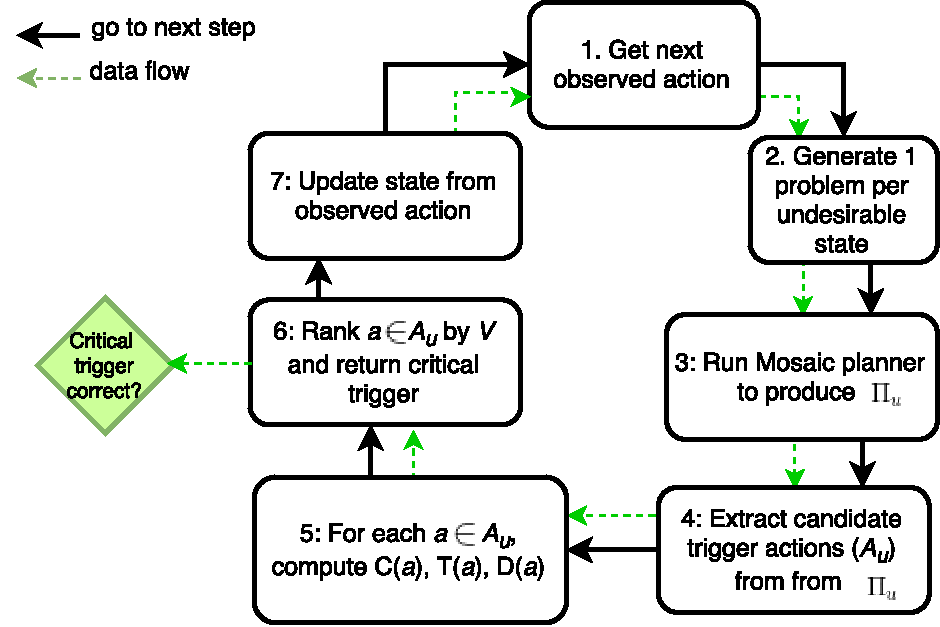
\includegraphics[width=0.7\textwidth]{img/algorithm.pdf}}
\caption{Seven-step process for determining whether an observed action is a critical trigger action.}
\label{fig:components}
\end{figure}

\section{Evaluating the Undesirable Consequence Recognition}
We examine which factors impact the performance of detecting critical trigger actions using our metric function $V$. The \emph{independent variables} of the study are summarized in Table~\ref{tab:exp}, and include the weights for V, the problems, the percentage of extraneous actions, and the percentage of actions ``removed'' to emulated partial observability.

Objective weights vary between a single metric, pairs of metrics and all three metrics with equal weights. We decided on these objective weight settings in order to identify which metrics (or their combinations) are sensitive to partial observability and extraneous actions separately. 


We begin with results from a user study on cyber-security that motivated our work. This domain will be referred to as the \texttt{PAG} in our evaluation. For traces from the user study, we examine the impact of the objective weights (OW) used for in the objective function. Noisy sensing can lead to extraneous actions or missed observations, which complicates intervention. So we generalize these results to a set of benchmark domains from \cite{ramirez2009plan}, where greater experimental control allows us to evaluate the impact of extraneous actions (EA) and partial observability (PO). Thus, we expect some degradation in performance as the noise increases and observability decreases; the question is by how much? 

\begin{table}[tpb]
\caption{Independent variables for evaluating impact of algorithm parameters and sensitivity to noisy data}
\label{tab:exp}
\begin{tabular}{|l|l|}
\hline
Variable                   & Settings                                           \\ \hline
\begin{tabular}[c]{@{}l@{}}Objective Weights (OW)\\ (C,T,D)\end{tabular} &
  \begin{tabular}[c]{@{}l@{}}(1,0,0), (0,1,0), (0,0,1), (0.33,0.33,0.33), (0.5,0.5,0), \\ (0.5,0,0.5), (0,0.5,0.5)\end{tabular} \\ \hline
Planning Domains (PD)       & PAG, blocks-words, navigator, ipc-grid+, logistics \\ \hline
Partial observability (PO) & 25\%, 50\%, 75\%, 100\%                            \\ \hline
Extraneous Actions (EA)    & 0\%, 50\%, 75\%, 100\%                             \\ \hline
\end{tabular}
\end{table}


The \emph{dependent variables} of the study include accuracy and computational overhead as measured in CPU time. For the cybersecurity domain, accuracy is defined as the percent true-positives only. For the benchmarks, we report accuracy in terms of percent true-positives and true-negatives. Computation time is included because ultimately we envision this being one component of a user supporting agent, which will require fast response. CPU time includes the time required to process each observation (one cycle of the process depicted in Figure~\ref{fig:components}) within a trial; this includes both generating the alternate plans and ranking the actions. 

For each undesirable state, we use a plan generated by an automated planner as the ground-truth undesirable plan. 
This is a fair assumption because the trace generation algorithm produces traces leading to the undesirable state (with varying levels of noise and observability). 
We measure accuracy with two evaluation metrics:
\begin{itemize}
\item Success rate in ignoring extraneous actions (Ignored EA)
\item Success rate in flagging undesirable actions that appear in the ground truth undesirable plan (Flagged UP)
\end{itemize}

Ignored EA for an observation trace is computed as the count of instances where the observation was an extraneous action and it was not flagged as a critical trigger (count EA). It is given by the equation:
\begin{equation}
\textup{Ignored EA}\%= \frac{\textup{count EA}}{\textup{number of extraneous actions in trace}}\times 100
\end{equation}
Flagged UP for an observation trace is computed as the count of instances where the observation was an action from UP and the function V actually selected it as the critical trigger action. It is given by the equation:
\begin{equation}
\textup{Flagged UP}\%= \frac{\textup{count UP}}{\textup{number of UP actions in trace}}\times 100
\end{equation}

\subsection{Cyber-security Domain (PAG)}
In Chapter~\ref{chap:ch3}, we discussed the findings of an human subject experiment where users performed routine computer tasks in a sandboxed simulation environment.
The objective of this study was to determine how non-expert users behave when presented with questionable computer security situations and to compare their actual observed behavior to their self-reports obtained via pre- and post-hoc surveys. 
Participants were presented with a desktop which includes common applications such as emailing, Web-browsing, social networking etc. 
They were also provided with written instructions on how to perform normal home computer user activities such as reading/sending email, installing software etc. While the normal computer activities were being performed, different events were simulated, without the subject's knowledge that can trigger threats and vulnerabilities of interest. 
These events included enticing user to disclose sensitive information (login names, passwords) to phishing sites over email and social media communications, responding to pop-ups asking the user to download a software, and reacting to malicious activities detected in the computer by an anti-virus program. 
Sixty-three human subjects participated in the study; their actions were collected into observation traces and will be used in the evaluation of our undesirable consequences recognition algorithm.


We constructed a PDDL domain for the Personalized Attack Graph (\texttt{PAG}) to investigate what actions subjects might take amid the aforementioned threat scenarios.  We considered four undesirable states for this domain, resulting in four problem definitions. Figure~\ref{fig:trace} shows an actual observation trace indicating how the subject's observed actions (x axis) contributed to triggering the four undesirable states (the plans to do so are displayed as a sequence in each color). The y-axis shows how many steps in each undesirable plan (UP) have yet to be executed. When the dots remain horizontal, the actions are not in the undesirable plan; they are extraneous. For this trace, although the subject came close to triggering all four, only one actually happened (red color line - virus scan vulnerability). 

\begin{figure}[tpb]
 \centerline{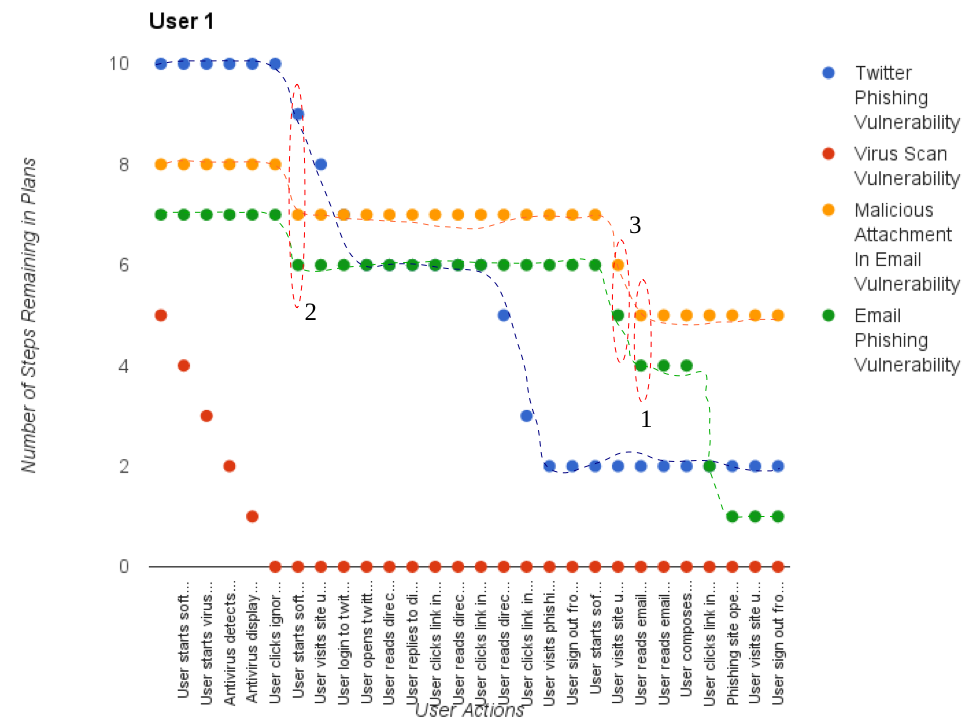
\includegraphics[width=\columnwidth, keepaspectratio=true]{img/user-study.png}}
 \caption{Observation trace from a human subject annotated with relation to undesirable plans (colored connected dots) and candidate trigger actions (in dotted ovals)}
 \label{fig:trace}
\end{figure}

We expected accuracy to be low because user logs offer unique challenges to the algorithm. Human users do not typically perform tasks in an ordered sequence. For example, some logs indicated that the subject was performing the same task repetitively, users had skipped a task to come back to it after an interval and more interestingly, some users were actively trying to trigger the vulnerabilities. These scenarios make it difficult to model a consistent state in a planning environment and affect candidate trigger actions being selected for the critical trigger ranking algorithm. To assess algorithm performance in a more controlled environment, we turned to benchmarks.


\subsubsection{PAG Results}
Since activity logs captured during the experiment could not be properly controlled for extraneous and missing actions, we limit the assessment to accuracy and the effect of the metric weightings on Flagged UP accuracy and CPU usage.

The subjects were only provided with instructions to perform normal computer tasks. No restrictions were imposed on how they should interact with desktop environment (e.g., undo/redo tasks, exploring application features). Therefore, subject's goals while performing the tasks were unknown. Logs generated by two subjects were discarded because they did not complete the experiment. Considering 61 traces used in this evaluation, mean trace length was 39 (SD=21.13). The longest trace contained 120 observations, while the shortest was 10. 


Mean Flagged UP accuracy was 59.53\% (SD=30.79) across all metric weight assignment classes, but the weights exerted a significant influence on accuracy (\textit{F}=40866, \textit{p}$\ll$0). 
The highest accuracy (mean=95.59\%,SD=2.13) occurred for two configurations of metric weight assignments: one that equally weighted Certainty, Desirability and Timeliness metrics as well as the one that equally weighted Certainty and Timeliness, ignoring the Desirability metric. 
We find that, in the cyber-security domain, the Undesirable Consequence Recognition algorithm relies on the Certainty and Timeliness metrics the most.
Mean CPU time per cycle of the algorithm was 1.7 seconds (SD=0.45), suggesting that this algorithm could easily be integrated into an agent that mitigates cyber-security issues.


\subsection{Benchmark Domains}
To generalize the results, we examine four domains from \cite{ramirez2009plan}. 
\sloppy
{\tt Block-Words} constructs one of 20 English words using 8 distinct letters. {\tt Grid-Navigation} forms paths through a connected graph to specific locations (goals). {\tt IPC-grid+} is a grid navigation with keys added at a restricted set of locations. {\tt Logistics} moves packages between locations. To keep the scale similar to the user study, we randomly selected four problems from each domain distribution.

\subsubsection{Trace Generation}
We choose four undesirable states for each benchmark domain.
To construct problem factors, partial observability and extraneous actions, we construct four planning problems with the undesirable states set as the goals. 
For each problem, we generate noisy traces by incrementally building the plan starting from the initial state and interleaving it with actions from a set of pre-computed extraneous actions when the current state meets the preconditions of the extraneous action. 
Thus, the trace generation algorithm consists of two stages (1) computing the set of extraneous actions (EA) and (2) interleaving these extraneous actions in to the trace. 
To construct partial observability (PO), actions from the original ground truth 
undesirable plan are randomly removed from the interleaved trace.

We use the Metric-FF planner \cite{hoffman2003ff} to generate extraneous actions because the planner's implementation offers configuration options to extract the relaxed planning graph and add/delete effects of actions. 
The challenge in generating extraneous actions is to ensure that they (1) do not introduce new facts that interfere with the progression of the ground-truth undesirable plan  or (2) does not delete the progress already made by the ground truth undesirable plan. 

First, we incrementally build the set of extraneous actions starting from selecting actions that can be executed immediately after the goal state has been reached. 
By adding new actions, object types, and predicates to the domain model, the size of the resulting extraneous action set can be increased to handle longer plans and create lengthy traces. 
The advantage of forward-expanding the set of extraneous actions starting at the goal state is that at this stage, the only condition we need to check is whether or not the chosen action deletes the goal state or not.
We add the actions that do not delete the goal state predicates as extraneous actions. 
It is also possible to select extraneous actions from the applicable actions in the current level of the Relaxed Planning Graph.
However, this does not guarantee that these actions will not violate conditions (1) and (2) later in the plan. 
In certain occasions selecting extraneous actions this way could lead to traces where the same action is being done and undone repeatedly without making progress through the plan, which is unrealistic and not rational behavior.

 
We designed a trace generation algorithm that overcomes the aforementioned problems and builds the ground-truth undesirable plan incrementally from the initial state, while interleaving it with extraneous actions.
Algorithm \ref{alg:extraneous} describes the process to compute the extraneous action pool for each problem in a domain.
\begin{algorithm}
    \caption{Extraneous Action Generation Algorithm}
    \label{alg:extraneous}
    \begin{algorithmic}[1]
        \Procedure{extraneouspool}{$domain$,$undesirableState,init$}
        	\State $current\gets UP, EX_{goal}\gets \emptyset, state \gets \emptyset$
        	\State $UP\gets Planner(domain,undesirableState,init)$
        	\State $state \gets init$
        	\ForAll{$a \in current$}
        		\If{$Pre(a)\in state $} 
        		\State $state\gets state\setminus Del(a)\cup Add(a)$
        		\EndIf
        	\EndFor
        	\State $S_{g}\gets state$
        	\State $RPG \gets RelaxedPlanningGraph(domain,undesirableState,init)$
        	\ForAll {$action \in RPG$}
				\If{$(action \notin UP) \And (Pre(action) \in S_{g}) \And (state \setminus Del(action) \cup Add(action) \cap S_{g} = \emptyset)$} 
				\State $EX_{g} \gets action$
				\EndIf        	        	
           	\EndFor
            \State \textbf{return} $EX_{g}$
        \EndProcedure
    \end{algorithmic}
\end{algorithm}
We begin by computing the ground-truth undesirable plan $UP$ using a planner. 
Then for the actions in $UP$ we modify the initial state by incorporating the effects of each action. 
The end of this loop translates the $state$ to the goal state for the problem. 
Then we generate the Relaxed Planning Graph for the planning problem with the goal equal to the undesirable state.
We select actions from the Relaxed Planning Graph such that the actions that are not already in $UP$ and the selected action is applicable in the goal state and post-conditions of the selected action do not remove any goal predicates. 
These actions form the extraneous action pool $EX_{g}$.
The set $EX_{g}$ needs to be extended because we evaluate the Undesirable Consequence Recognition algorithm by varying the percentage of extraneous actions in the observation trace.
This is done by modifying $S_{g}$ with effects of a selected action from $EX_{g}$, and repeating steps 4 through 5. 
The intuition is that once an extraneous action is executed at some state, the resulting state may enable additional extraneous actions. 
Repeat execution of this process generates a tree structure of extraneous actions with an action from $EX_{g}$ as root. 

For an observation trace, we define the metric percent extraneous actions (EA) as follows:
\begin{equation}
\textup{percent extraneous actions (EA)} = \frac{\textup{number of extraneous actions in trace}} {\textup{number of actions in plan}}
\end{equation} 
This metric is used as a proxy for signal-to-noise ratio $[$0\%, 50\%, 75\%, 100\%$]$. 
Algorithm \ref{alg:noisytrace} describes our trace generation process. 
Starting from the initial state, actions in the undesirable plan are added to the observation trace sequentially, including extraneous actions as appropriate. 
This produces a final plan. 
Partial observability (PO) is computed by randomly removing actions from the final plan such that, PO\% (number of original actions in trace after removal / number of original actions in trace before removal) is one of $[$25\%, 50\%, 75\%, 100\%$]$. 

\begin{algorithm}
    \caption{Noisy Observation Trace Generation Algorithm}
    \label{alg:noisytrace}
    \begin{algorithmic}[1] % The number tells where the line numbering should start
        \Procedure{noisytrace}{$domain$,$problem,init$}
        	\State $current\gets UP, ea\gets 0, trace\gets \emptyset, state \gets init$
        	\State $UP\gets Planner(domain,problem,state)$
        	\ForAll{$a \in current$}
        		\If{$Pre(a)\in state $} 
        		\State $trace \gets trace \cup a$
        		\State $state\gets state\setminus Del(a)\cup Add(a)$
        		\EndIf
        		\State $UP\gets Planner(domain,problem,state)$
        		\State $current\gets UP$
        		\If {$ea<required EA\%$}
        		\State randomly select $action$ from $EX_{goal}$ if Pre($action$) $\in state$
        		\State $trace \gets trace \cup action$
        		\State update $ea, state, current$
        		\EndIf
        	\EndFor
        	\State Fix PO\% in $trace$ by removing actions
            \State \textbf{return} $trace$
        \EndProcedure
    \end{algorithmic}
\end{algorithm}





   \begin{table}[tpb]
     \centering
   \begin{small}
   	\caption{Mean Ignored EA\%  (and standard deviation) for benchmark domains for levels of EA\% in observation trace and objective weight assignment classes. The left three columns combine mean Ignored EA\% for OW assignments across all values of $\alpha$ and breaks mean Ignored EA\% down by EA\% in trace. The right OW columns breaks down mean Ignored EA\% by specific $\alpha$ value for all levels of EA\% in observation trace.}
	\label{tab:ignoredeaforlevels}
   \resizebox{\columnwidth}{!}{
	\begin{tabular}{|c|ccc|ccccccc|}
		\hline
	    & \multicolumn{10}{c|}{Mean Ignored EA\%} \\ \cline{2-11}
		\multirow{3}{*}{Domain}  & \multicolumn{3}{c|}{EA\% in trace} & \multicolumn{7}{c|}{OW Assignments  (C,T,D)} \\ \cline{2-11} 
		& 50\% & 75\% & 100\%
%		& (0,0,1) & (0,.5,.5) & (0,1,0) & (.3,.3,.3) & (.5,0,.5) & (.5,.5,0) & (1,0,0) \\ \hline
		& (0,0,1) & (0,0.5,0.5) & (0,1,0) & (0.3,0.3,0.3) & (0.5,0,0.5) & (0.5,0.5,0) & (1,0,0) \\ \hline
		\texttt{blo} & \begin{tabular}[c]{@{}c@{}}95.2 \\ (8.0)\end{tabular} & \begin{tabular}[c]{@{}c@{}}97.6\\ (3.6)\end{tabular} & \begin{tabular}[c]{@{}c@{}}97.3\\ (3.2)\end{tabular} & \begin{tabular}[c]{@{}c@{}}99.0\\ (1.6)\end{tabular} & \begin{tabular}[c]{@{}c@{}}94.7\\ (6.7)\end{tabular} & \begin{tabular}[c]{@{}c@{}}95.2\\ (6.2)\end{tabular} & \begin{tabular}[c]{@{}c@{}}95.4\\ (7.0)\end{tabular} & \begin{tabular}[c]{@{}c@{}}98.6\\ (1.7)\end{tabular} & \begin{tabular}[c]{@{}c@{}}95.4\\ (7.0)\end{tabular} & \begin{tabular}[c]{@{}c@{}}98.6\\ (1.7)\end{tabular} \\ \hline
		\texttt{ipc} & \begin{tabular}[c]{@{}c@{}}86.4\\ (14.4)\end{tabular} & \begin{tabular}[c]{@{}c@{}}89.9\\ (11.6)\end{tabular} & \begin{tabular}[c]{@{}c@{}}89.9\\ (10.7)\end{tabular} & \begin{tabular}[c]{@{}c@{}}95.6\\ (3.7)\end{tabular} & \begin{tabular}[c]{@{}c@{}}83.2\\ (13.0)\end{tabular} & \begin{tabular}[c]{@{}c@{}}81.3\\ (12.9)\end{tabular} & \begin{tabular}[c]{@{}c@{}}83.9\\ (15.1)\end{tabular} & \begin{tabular}[c]{@{}c@{}}95.9\\ (3.4)\end{tabular} & \begin{tabular}[c]{@{}c@{}}85.1\\ (14.8)\end{tabular} & \begin{tabular}[c]{@{}c@{}}95.9\\ (3.4)\end{tabular} \\ \hline
		\texttt{log} & \begin{tabular}[c]{@{}c@{}}97.9 \\ (4.4)\end{tabular} & \begin{tabular}[c]{@{}c@{}}96.7\\ (5.7)\end{tabular} & \begin{tabular}[c]{@{}c@{}}96.1\\ (5.4)\end{tabular} & \begin{tabular}[c]{@{}c@{}}98.4\\ (2.8)\end{tabular} & \begin{tabular}[c]{@{}c@{}}94.4\\ (7.2)\end{tabular} & \begin{tabular}[c]{@{}c@{}}96.1\\ (3.6)\end{tabular} & \begin{tabular}[c]{@{}c@{}}96.2\\ (6.9)\end{tabular} & \begin{tabular}[c]{@{}c@{}}98.6\\ (2.6)\end{tabular} & \begin{tabular}[c]{@{}c@{}}96.2\\ (6.9)\end{tabular} & \begin{tabular}[c]{@{}c@{}}98.5\\ (2.6)\end{tabular} \\ \hline
		\texttt{nav} & 100 (0) & 100 (0) & 100 (0) & 100 (0) & 100 (0) & 100 (0) & 100 (0) & 100 (0) & 100 (0) & 100 (0) \\ \hline
	\end{tabular}
	}%	
   \end{small}
\end{table}


\begin{table}[tpb]
	\centering
\begin{small}
\caption{Mean Flagged UP\%  (and standard deviation) for benchmark domains for levels of PO\% in observation trace and objective weight assignment classes. The left four columns combine mean Flagged UP\% for OW assignments across all values of $\alpha$ and breaks mean Flagged UP\% down by PO\% in trace. The right OW columns breaks down mean Flagged UP\% by specific $\alpha$ value for all levels of PO\% in observation trace.}
	\label{tab:flaggedupforlevels}
\resizebox{\columnwidth}{!}{
	\begin{tabular}{|c|c c c c|c c c c c c c|}
		\hline
		& \multicolumn{11}{c|}{Mean Flagged UP\%} \\ \cline{2-12} 
		\multirow{3}{*}{Domain} & \multicolumn{4}{c|}{PO\% in trace} & \multicolumn{7}{c|}{OW Assignments (C,T,D)} \\ \cline{2-12} 
%		& 25\% & 50\% & 75\% & 100\% & (0,0,1) & (0,.5,.5) & (0,1,0) & (.3,.3,.3) & (.5,0,.5) & (.5,.5,0) & (1,0,0) \\ \cline{1-12} 
		& 25\% & 50\% & 75\% & 100\% & (0,0,1) & (0,0.5,0.5) & (0,1,0) & (0.3,0.3,0.3) & (0.5,0,0.5) & (0.5,0.5,0) & (1,0,0) \\ \cline{1-12} 
		
		\texttt{blo} & \begin{tabular}[c]{@{}c@{}}20.1\\ (21.2)\end{tabular} & \begin{tabular}[c]{@{}c@{}}23.6\\ (14.4)\end{tabular} & \begin{tabular}[c]{@{}c@{}}31.8\\ (19.3)\end{tabular} & \begin{tabular}[c]{@{}c@{}}40.2\\ (26.1)\end{tabular} & \begin{tabular}[c]{@{}c@{}}9.2\\ (7.6)\end{tabular} & \begin{tabular}[c]{@{}c@{}}24.8\\ (20.1)\end{tabular} & \begin{tabular}[c]{@{}c@{}}37.0\\ (17.5)\end{tabular} & \begin{tabular}[c]{@{}c@{}}46.5\\ (24.9)\end{tabular} & \begin{tabular}[c]{@{}c@{}}19.0\\ (7.6)\end{tabular} & \begin{tabular}[c]{@{}c@{}}46.8\\ (24.9)\end{tabular} & \begin{tabular}[c]{@{}c@{}}19.0\\ (7.6)\end{tabular} \\ \hline
		\texttt{ipc} & \begin{tabular}[c]{@{}c@{}}6.9\\ (18.8)\end{tabular} & \begin{tabular}[c]{@{}c@{}}25.6\\ (20.0)\end{tabular} & \begin{tabular}[c]{@{}c@{}}42.3\\ (32.0)\end{tabular} & \begin{tabular}[c]{@{}c@{}}50.8\\ (36.2)\end{tabular} & \begin{tabular}[c]{@{}c@{}}9.7\\ (5.2)\end{tabular} & \begin{tabular}[c]{@{}c@{}}46.5\\ (34.7)\end{tabular} & \begin{tabular}[c]{@{}c@{}}47.9\\ (35.0)\end{tabular} & \begin{tabular}[c]{@{}c@{}}47.5\\ (35.8)\end{tabular} & \begin{tabular}[c]{@{}c@{}}10.5\\ (4.9)\end{tabular} & \begin{tabular}[c]{@{}c@{}}47.1\\ (35.9)\end{tabular} & \begin{tabular}[c]{@{}c@{}}10.6\\ (4.9)\end{tabular} \\ \hline
		\texttt{log} & \begin{tabular}[c]{@{}c@{}}18.4\\ (27.4)\end{tabular} & \begin{tabular}[c]{@{}c@{}}16.4\\ (20.1)\end{tabular} & \begin{tabular}[c]{@{}c@{}}20.4\\ (19.5)\end{tabular} & \begin{tabular}[c]{@{}c@{}}31.5\\ (17.8)\end{tabular} & \begin{tabular}[c]{@{}c@{}}15.2\\ (10.6)\end{tabular} & \begin{tabular}[c]{@{}c@{}}20.9\\ (28.2)\end{tabular} & \begin{tabular}[c]{@{}c@{}}24.6\\ (25.4)\end{tabular} & \begin{tabular}[c]{@{}c@{}}27.2\\ (28.5)\end{tabular} & \begin{tabular}[c]{@{}c@{}}18.3\\ (10.1)\end{tabular} & \begin{tabular}[c]{@{}c@{}}27.2\\ (28.5)\end{tabular} & \begin{tabular}[c]{@{}c@{}}18.3\\ (10.9)\end{tabular} \\ \hline
		\texttt{nav} & \begin{tabular}[c]{@{}c@{}}14.8\\ (19.1)\end{tabular} & \begin{tabular}[c]{@{}c@{}}32.4\\ (22.6)\end{tabular} & \begin{tabular}[c]{@{}c@{}}45.2\\ (27.4)\end{tabular} & \begin{tabular}[c]{@{}c@{}}61.7\\ (39.8)\end{tabular} & \begin{tabular}[c]{@{}c@{}}14.1\\ (3.4)\end{tabular} & \begin{tabular}[c]{@{}c@{}}56.8\\ (33.7)\end{tabular} & \begin{tabular}[c]{@{}c@{}}56.8\\ (33.7)\end{tabular} & \begin{tabular}[c]{@{}c@{}}56.8\\ (33.7)\end{tabular} & \begin{tabular}[c]{@{}c@{}}14.1\\ (3.43)\end{tabular} & \begin{tabular}[c]{@{}c@{}}56.8\\ (33.7)\end{tabular} & \begin{tabular}[c]{@{}c@{}}14.1\\ (3.4)\end{tabular} \\ \hline
	\end{tabular}
	}%
\end{small}
\end{table}



\subsubsection{Benchmark Results}
We review the overall accuracy of our algorithm in benchmark domains by evaluating how well it ignores extraneous actions and flags undesirable actions in the ground truth plan.

\textbf{Ignoring Extraneous Actions}\\
When encountered with extraneous actions in the trace, the algorithm must be able to avoid flagging it as critical. We define mean Ignored EA\% percentage for a domain as: (sum of Ignored EA\% per trial / number of trials with EA\%$>$0). Table \ref{tab:ignoredeaforlevels} shows how mean Ignored EA\% varies with the noise level of the observation trace and objective weight assignments.

Results show that our algorithm consistently ignores extraneous actions for all benchmark domains. This high accuracy rate can be attributed to our process of selecting critical trigger actions. Since candidate trigger actions are extracted from a set of alternative plans leading to the same undesirable state, the likelihood of true extraneous actions to appear in the set of alternative plans is low. This reduces the likelihood of false-positives in the trace.


The OW combinations significantly influence Ignored EA\%  ($p<0.05$ for the \texttt{blo}, \texttt{ipc} and \texttt{log} domains). Post-hoc analysis using TukeyHSD at $\alpha=0.05$ shows that across domains, OW combinations that do not consider the timeliness metric better perform at ignoring extraneous actions than combinations that include timeliness. This is because timeliness metric is not sensitive to extraneous actions in the trace. As a result, the objective function can not sufficiently differentiate between extraneous actions and actions in ground truth plan, leading to false positives.Because timeliness metric captures progress yet to be made from current state to triggering the undesirable state in terms of remaining steps, in the presence of extraneous actions, which do not contribute to progress toward the undesirable state, the metric does not sufficiently demote the extraneous action in the candidate action set, leading to false-positives. 
In contrast, certainty and desirability metrics look for occurrences of an action in undesirable plans. As extraneous actions do not occur in undesirable plans, both metrics are capable of filtering extraneous actions from the candidate action pool by minimizing objective function value and preventing them from being selected as the critical trigger.


\textbf{Flagging Undesirable Actions}\\
Flagged UP\% captures how well the algorithm flags observations as critical triggers given that the observation appears in an undesirable plan treated as ground truth. We first look at Flagged UP\% in traces with 0\% noise and full observability (i.e., best-case scenario) to establish an upper bound to the metric.

Table \ref{tab:flagupupperbound} shows a very large range (Max-Min) for Flagged UP\%. This indicates that although the only variable for this sample is OW, Flagged UP\% is also sensitive to other external factors that have not been accounted for in our proposed objective function. The challenge lies in identifying these external factors and determining their relationship so that the objective function can be tuned to improve accuracy. This will be the main focus of our future work. 

Table \ref{tab:flaggedupforlevels} shows that Flagged UP\% also increases when observability increases in the trace. Factor analysis using one-way ANOVA for OW shows that this positive effect is significant ($p<0.05, df=6$) for all four benchmark domains. Interestingly, high Flagged UP\% was reported for OW combinations that consider timeliness: specifically for configurations, certainty-timeliness-desirability with equal weighting, certainty-timeliness with equal weighting and desirability-timeliness with equal weighting. Post-hoc analysis using TukeyHSD at $\alpha=0.05$ shows that this difference is significant. Thus, we conclude that the timeliness metric can improve the true-positive rate, yielding higher precision for the algorithm. The timeliness metric is sensitive to partial observability because it sufficiently captures distance to triggering an undesirable state, which is a consistent indicator of the progress is being made. Even with partial observability, the remaining steps of a plan change in such a way that it can be tracked and correctly reflected in the objective function. Accuracy of the certainty and desirability metrics lowers as partial observability increases because they consider occurrences of an action. 


\textbf{Computational Overhead}\\
For each benchmark domain, we calculated the average CPU time per cycle for problem factors (EA and PO). As shown in Table \ref{tab:cpu2}, we found differences due to observation trace factors; two-way ANOVA on EA and PO showed significant main effects and interaction effects ($p<$0.05) for \texttt{ipc}, \texttt{log} and \texttt{nav} domains.


\begin{table}[tpb]
  \centering
    \caption{Mean CPU time in seconds for problem factors for each domain. $\Delta$ is the difference between the max and min times for each domain.}
  \label{tab:cpu2}
    \resizebox{0.7\columnwidth}{!}{
  \begin{tabular}{|l|r|r|r|r|r|r|r|r|r|}
    \hline
    \multirow{2}{*}{Domain}
  &  \multicolumn{4}{c|}{EA\% in trace} & \multicolumn{4}{c|}{PO\% in trace} & \\ \cline{2-9}
 & 0\% & 50\% & 75\% & 100\% & 25\% & 50\% & 75\% & 100\% & $\Delta$ \\
    \hline
{\tt blo} & 2.3  & 2.2  & 2.2  & 2.2  & 2.2  & 2.2  & 2.3  & 2.2  & 1.4  \\
{\tt ipc} & 4.9  & 4.8  & 4.9  & 4.9  & 4.9  & 4.9  & 4.9  & 4.8  & 0.9  \\
{\tt log} & 1.7  & 1.7  & 1.6  & 1.7  & 1.7  & 1.7  & 1.7  & 1.7  & 0.5  \\
{\tt nav} & 1.3  & 1.3  & 1.3  & 1.3  & 1.3  & 1.3  & 1.3  & 1.3  & 0.5  \\
    \hline
  \end{tabular}
  	}%resize box
\end{table}

\begin{table}[tpb]
	\centering
\caption{Flagged UP\% for traces with 0\% EA and 100\% PO for \texttt{Block-words} (\texttt{bw}), \texttt{IPC-grid+} (\texttt{ipc}), \texttt{Logistics} (\texttt{log}), and \texttt{Grid-Navigation}   (\texttt{nav}) domains}
		\label{tab:flagupupperbound}
    \begin{small}
	\begin{tabular}{|l|c|c|c|c|}
		\hline
		\multirow{2}{*}{Domain} & \multicolumn{4}{c|}{Flagged UP\%} \\ \cline{2-5} 
		& Mean   & SD     & Min    & Max    \\ \hline
		\texttt{blo}                     & 37.12  & 24.83  & 6.12   & 77.78  \\ 
		\texttt{ipc}                     & 43.27  & 30.55  & 0.00   & 90.00  \\ 
		\texttt{log}                     & 31.77  & 17.27  & 12.82  & 66.67  \\ 
		\texttt{nav}                     & 61.68  & 40.31  & 14.10  & 100.00 \\ \hline
	\end{tabular}
\end{small}

\end{table}

\section{Concluding Remarks}
We have described a variant of plan recognition that can help identify intervention points to help a user avoid undesirable states while interacting with a computer. Our approach views the decision of when to intervene as a multi-objective optimization problem that optimizes three domain-independent  metrics: certainty, timeliness and desirability. We tested our algorithm on both benchmark domains and human subject data from a cyber-security experiment. Results show that, across all benchmark domains, certainty and desirability metrics perform well in ignoring extraneous actions, while the timeliness metric and it's combinations with certainty and desirability perform well in identifying true positives. We identified two metrics that are sensitive to noise in action based observation traces and a metric that is sensitive to partial observability of actions.

However, the low percentage of true-positives in the best case scenario indicate that the metrics are not good enough in their raw form in dealing with partial observability. Therefore, metrics must be developed to evaluate the contribution of less frequent actions appearing in alternative plans. Evaluation of the effects of objective weight metrics, shows that desirability metric does not adequately downgrade the effect of certainty and timeliness. This indicates that objective weight assignments require an in depth look into multi-objective optimization techniques to find the optimal combination of weights over metrics.


\chapter{Balancing Safety and Freedom for the User: Intervention as Planning and Human-aware Intervention}
\label{chap:ch5}
When working in an unfamiliar online environment,  it can be helpful to have an observer that can intervene and guide a user toward a desirable outcome while avoiding undesirable outcomes or frustration.
The {\em Intervention Problem} is deciding when to intervene in order to help a user.
The Intervention Problem is similar to, but distinct from Plan Recognition because the observer must not only recognize the intended goals of a user but also when to intervene to help the user, but also to only intervene when necessary.
We formalize a family of Intervention Problems and show how these problems can be solved using a combination of Plan Recognition methods and classification techniques to decide whether to intervene.
The dimensions of the Intervention Problem presented in this chapter are summarized in Table~\ref{tab:dim3}

\begin{table}[ptb]
\begin{tabular}{|l|l|}
\hline
\textbf{Dimension} & \textbf{Domain Specific Properties} \\ \hline
Actors in the environment & User, Competitor (optional), Observer \\ \hline
Goals hidden to the observer & \begin{tabular}[c]{@{}l@{}}User's goal not hidden\\ One or more known undesirable states\end{tabular} \\ \hline
Types of observations & The user's and the competitor's (if present) actions \\ \hline
Noise in observations & None \\ \hline
Intervention recovery & Offer helpful hint \\ \hline
\end{tabular}
\caption{Dimensions of the Unsafe Suffix Recognition Problem}
\label{tab:dim3}
\end{table}


We characterize the observer’s decision space as an Intervention Graph and 
construct it using an ``Intervention as Classical Planning'' approach to generate potential suffixes of partially executed plans.
We extract domain-independent features from this graph and extend several Plan Recognition benchmarks to evaluate this approach.
For our benchmarks, the learned models dominate three recent Plan Recognition approaches.
We then generalize these results to Human-Aware Intervention, 
where the observer must decide in real time whether to intervene for human users solving a cognitively engaging puzzle.
Using a revised feature set more appropriate to human behavior, 
we produce a learned model to recognize when a human user is about to trigger an undesirable outcome. 
We perform a human-subject study to evaluate the Human-Aware Intervention.
We find that the revised model also dominates existing Plan Recognition algorithms in predicting Human-Aware Intervention.


%===========================================================================================================
%%===========================================================================================================
\section{Introduction}
\noindent Even the best plan can go wrong. 
Dangers arise from failing to execute a plan correctly or as a result of actions executed by a nefarious agent. 
Consider route planning where a driver is unaware of upcoming road damage or a traffic jam. 
Or consider cyber-security where a user is unaware of an unsafe hyperlink. 
In both, plans achieving the desirable goal have similar prefixes to those that result in undesirable outcomes.
Suppose an observer watches the actions of a user working in a risky environment where plans may be subverted to reach an undesirable outcome. 
We study the problem of how the observer decides whether to intervene if the user appears to need help or the user is about to take an action that leads to an undesirable outcome.

We introduce \textit{Plan Intervention} as a new computational problem and relate it to plan recognition. 
To intervene, the observer needs to make a decision whether or not the user's likely plan will avoid the undesirable state. 
Thus, it is possible to argue that if the observer implements an existing state-of-the-art plan recognition algorithm (e.g., Plan Recognition as Planning \cite{ramirez2009plan}), then intervention can take place when the likely goal of the recognized plan satisfies the undesirable state. 
We show that the Intervention Problem carries subtleties that the state-of-the-art Plan Recognition Algorithms are not yet able to handle.
We propose two complementary solutions for Plan Intervention: (1) Unsafe Suffix Intervention and (2) Human-aware Intervention. 
We show that these two complementary solutions dominate state-of-the-art plan recognition algorithms in correctly recognizing when intervention is required.

For intervention, giving goal priors, as required for goal/plan recognition, is difficult because certain facts about the domain are hidden to the user and unintended goals may be enabled during execution regardless the priors. 
Furthermore, human actors may not construct plans the same way as an automated planner because humans may identify the optimal choice of actions every time. 
They may  make mistakes early on during tasks having a steep learning curve. 
Partial knowledge about the domain may preclude the human user from knowing the full effects of his actions or he may not be thinking about the effects at all. 
Therefore, the observer may not may not always be able to accurately estimate what the users are trying to do.

We study two kinds of Intervention Problems. 
In \emph{Unsafe Suffix Intervention}, the observer uses automated planners to project the remaining suffixes and extract features that can differentiate between safe and unsafe plans. 
We evaluate the recognition accuracy of Unsafe Suffix Intervention on benchmark planning problems. 
In \emph{Human-aware Intervention}, the observer uses the observed partial solution to extract features that can separate safe and unsafe solutions. 
We evaluate the accuracy of Human-aware Intervention on a new Intervention Planning benchmark called Rush Hour.


The contributions of this chapter are:
\begin{itemize}
\item formalizing the online Intervention Problem for determining when the potential of possible damage  of a state warrants interruption.
\item modeling the observer's decision space as an Intervention Graph, which can be constructed explicitly or sampled with an automated planner.
\item defining features to assess the criticality of a state using the Intervention Graph and the sampled plans.
\item extending existing benchmarks by Ramirez~\&~Geffner~ \citeyear{ramirez2009plan, ramirez2010probabilistic} to incorporate Intervention and  evaluating our intervention approach for the extended benchmarks.
\item introducing a new Plan Intervention benchmark domain called \emph{Rush Hour}, where a player moves vehicles arranged on a grid to clear a path for a target vehicle. 
\item formalizing the Human-aware Intervention Problem for the Rush Hour planning task and designing features to estimate the criticality using behavior features derived from the observed partial plan.
\item presenting the results from a human-subjects study where we collected human behavior on Rush Hour.
\item extending an existing plan recognition model to the Intervention Problem and demonstrating that three state-of-the-art plan recognition algorithms do not perform well in Intervention Problems.
\item training and evaluating the classification models using Rush Hour puzzle solutions collected from a human subject experiment and showing that the approach works well for the Rush Hour problem.
\end{itemize}

In this chapter, we first define a general form of the Intervention Problems and introduce three variants: (1) Intervention for a Single User, (2) Intervention in the Presence of a Competitor and (3) Human-aware Intervention. Next, we present approaches for Intervention for a Single User and Intervention in the Presence of a Competitor, both of which use the Intervention Graph and the sampled plans to recognize unsafe suffixes. We evaluate these two approaches against the state-of-the-art plan recognition algorithms on using benchmark planning domains in the benchmarks. Next, we present Human-aware Intervention, that uses machine learning to learn properties of the observed partial plans, as opposed to projecting suffixes, to determine when intervention is required. To evaluate Human-aware Intervention, we introduce a new planning domain called Rush Hour and study how human users solve Rush Hour puzzle as a planning task. We evaluate Human-aware Intervention in the Rush Hour domain compared to state-of-the-art plan recognition algorithms. We conclude the chapter with a discussion on why plan recognition falls short in solving Intervention Problems and present the open questions for future research in designing intervention models.


%%%===========================================================================================================
%%%===========================================================================================================
\section{The Intervention Environment}
\label{sec:distinguishing}
We model {\bf intervention} in environments where a \textit{user} is trying to achieve desirable goal(s), denoted \desired, while avoiding undesirable outcomes, denoted \undesired.
Note that in contrast to the Intervention Problem discussed in Chapter~\ref{chap:ch4}, the observer has knowledge about \desired and \undesired and must take into account both these goal states in order to make the intervention decision.
Some environments include a \textit{competitor} who may also take actions in the world, but we assume the user is not aware of the competitor's actions, as might happen in cyber-security applications.

We define the \textit{observer} to be the intervening assistant agent. 
An \textit{observer} receives each action and decides whether to forward the action to the execution platform;
this allows the observer to intervene if the action would result in the undesired outcome \undesired.  
The observer holds a history of previous observations $H = (o_1, o_2, \ldots, o_{i-1})$ that indicate the actions executed by the user or competitor.
The user presents the next action as an observation $o_{i}$ to the observer and the observer must decide ``should I intervene?''
This decision necessitates projecting what the observer knows and determining whether the user is about to do something unsafe (\undesired) 
or is moving too far away from a desirable goal (\desired).
We call such a projection a \textit{suffix}.
We denote a single  \textit{suffix} projection as \Suffix and the set of projections as \Suffixes because there will usually be many projections.

  
The intervention models discussed in Chapters~\ref{chap:ch4} and \ref{chap:ch5} emphasize on analyzing the remaining suffixes to decide when to intervene.
In Plan Recognition, the observer uses an observation trace $O$ to derive the user's likely plan. $O$ can be either an ordered sequence of actions  \cite{ramirez2009plan,ramirez2010probabilistic} or an ordered sequence of states \cite{sohrabi2016plan}.
In the first form of intervention we present in this chapter, the observer considers the remaining plans (i.e., suffixes) in safe and unsafe partitions to learn to recognize unsafe suffixes in order to help the user avoid \undesired. 
In this case, the observer can help the user by only accepting actions into \historyDef that will safely advance the user toward \desired.
We call the first intervention model, \textit{Unsafe Suffix Intervention}.
In the second form of intervention, the observer learns to recognize that the user is not making progress toward \desired by analyzing the \historyDef when a suffix is not available. In this case,  the observer must offer enough help to \textit{guide} the user toward \desired without giving the solution. 
The second intervention model is particularly useful when the user is a human and it can be difficult to evaluate progress with heuristics like a normal planning agent.
Therefore, we call the second intervention model, \textit{Human-aware Intervention}.
Plan Recognition does not define a method for the user to recover when the observer recognizes a plan leading to \undesired. 
With the proposed intervention models, we address that limitation with two different types of help the observer can offer to the user.

\section{Intervention Examples}

We will present two examples for \textit{Unsafe Suffix Intervention}.
The Grid Navigation domain example is used to illustrate intervention with the user and observer. 
In the grid navigation task illustrated in Figure~\ref{fig:single}, the user navigates from \texttt{W1} to \texttt{Z3} by moving vertically and horizontally and \texttt{Y3} contains a pit the user can not see: \mbox{$\desired=$ \texttt{(AT Z3)}} and \mbox{$\undesired=$ \texttt{(AT Y3)}}. 
Plans corresponding to paths A, B, C are all feasible solutions to the user's planning task. 
However, plans B and C are unsafe because they satisfy $\lbrace\dandu\rbrace$. 

\begin{figure}[tpb]
        \centering{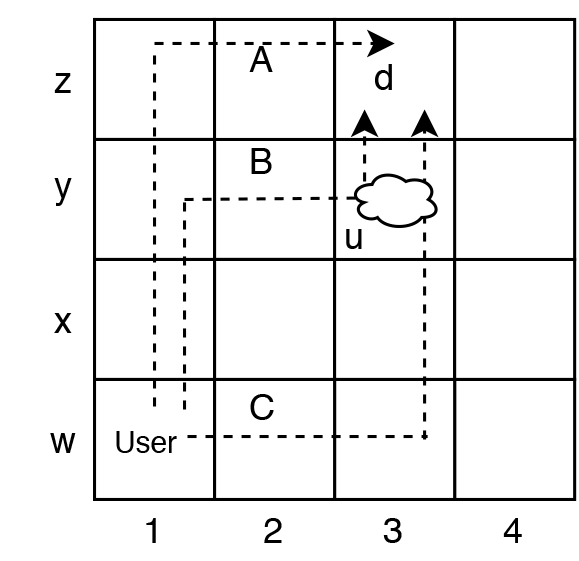
\includegraphics[width=0.3\columnwidth]{img/figure1.jpg}}
         \vspace{-1em}
        \caption{Intervention modeled in the Grid Navigation domain}
        \vspace{-1em}
        \label{fig:single}
\end{figure}


Table~\ref{tab:prpgrid} shows how an observer modeled as an offline Plan Recognition agent will recognize the goals given observations $O$ for the Grid Navigation problem in Figure~\ref{fig:single}. Let us assume that the observer implements the Plan Recognition as Planning algorithm introduced by Ramirez et al. \citeyear{ramirez2010probabilistic} to disambiguate between \undesired and \desired. They show that the most likely goal will be the one that minimizes the cost difference $c(\mathrm{g}|O)-c(\mathrm{g}|\overline{O}), \mathrm{g}\in \lbrace\desired,\undesired\rbrace$. For each incrementally revealed $O$ (shown in columns), assuming uniform goal priors, the observer finds the most likely goal that agrees with $O$. For the cost computation, we assumed that the user is following a satisfising plan to achieve goals. 
It can be seen that for the Grid Navigation example, the observer can not correctly disambiguate between \desired and \undesired. 
More importantly, the final last column satisfies \undesired. At this point, it will be too late for the user to avoid \undesired.
Furthermore, because the observer accepts $O$ as is for Plan Recognition, the observer can not guide the user away from \undesired as the observations are already satisfied in the state.

\begin{table}[t]
\begin{tabular}{|c|l|l|l|l|}
\hline
$O$ & (\textsc{\texttt{move w1 x1}}) & \begin{tabular}[c]{@{}l@{}}(\textsc{\texttt{move w1 x1}}\\ \textsc{\texttt{move x1 y1}})\end{tabular} & \begin{tabular}[c]{@{}l@{}}(\textsc{\texttt{move w1 x1}}\\ \textsc{\texttt{move x1 y1}}\\ \textsc{\texttt{move y1 y2}})\end{tabular} & \begin{tabular}[c]{@{}l@{}}(\textsc{\texttt{move w1 x1}}\\ \textsc{\texttt{move x1 y1}}\\ \textsc{\texttt{move y1 y2}}\\ \textsc{\texttt{move y2 y3}})\end{tabular} \\ \hline
\begin{tabular}[c]{@{}l@{}}$c(\mathrm{u}|O)-c(\mathrm{u}|\overline{O})$\end{tabular} & $4 - 4 = 0$ & $4 - 4 = 0$ & $4 - 4 = 0$ & $4 - 4 = 0$ \\ \hline
\begin{tabular}[c]{@{}l@{}}$c(\mathrm{d}|O)-c(\mathrm{d}|\overline{O})$\end{tabular} & $5 - 5 = 0$ & $5 - 5 = 0$ & $5 - 5 = 0$ & $5 - 5 = 0$ \\ \hline
Most likely goal & No decision & No decision & No decision & Fail \\ \hline
\end{tabular}
\caption{Observer modeled as a Plan Recognition agent for the Grid Navigation example in Figure~\ref{fig:single}}
\label{tab:prpgrid}
\end{table}

\begin{figure}[tpb]
 \centering{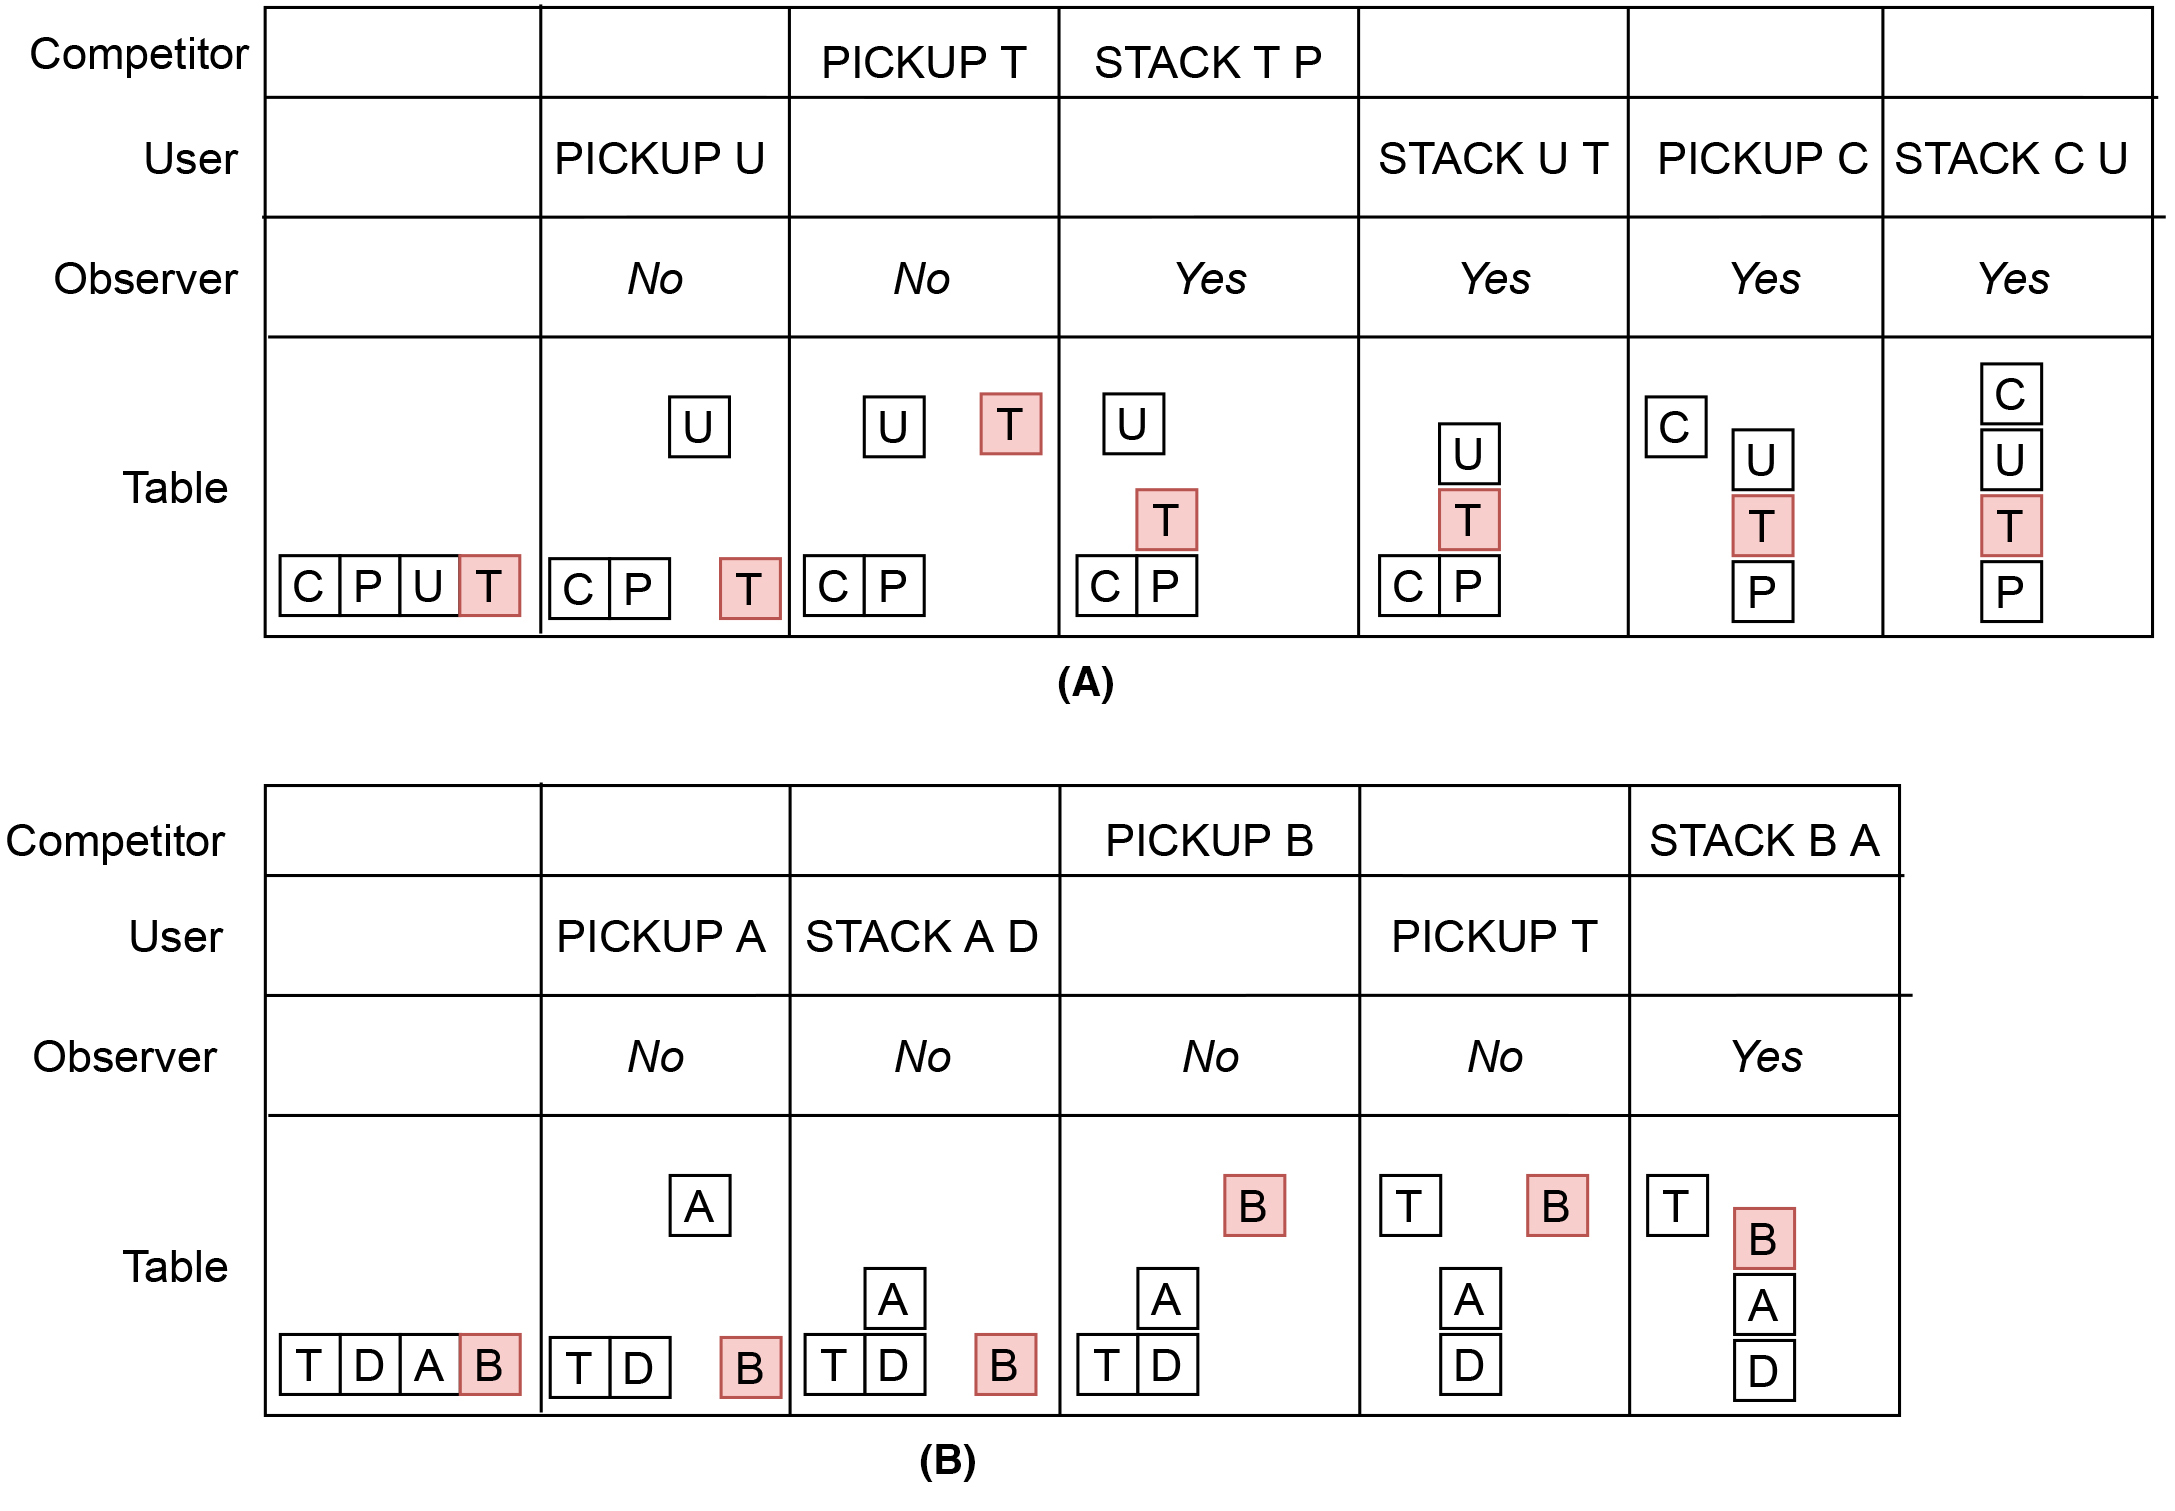
\includegraphics[width=0.7\columnwidth]{img/figure2.jpg}}
   \caption{(A) User and competitor intervention modeled in the Blocks Words domain, where $\undesired=$ (CUT) and $\desired=$ (CUP). (B) User and competitor intervention where $\undesired= $ (BAD) and $\desired= $ (TAD). \\ Initially, all four blocks are on the table. An action in the user or competitor row indicates the Intervention Suffix. The \textit{Yes} label in the observer's row indicates that intervention is required. The \textit{No} label indicates that intervention is not required.}
\label{fig:bw2}
\end{figure}

Now let us consider a situation where there may be some additional agent taking actions in the world.
For example, in a cyber-security application, a second agent may insert malicious code in a file to gain access to a privileged information.
More generally, we call this additional agent a competitor, since it is not always the case that they are ``attacking'' a user.
The Blocks Word domain example from Ramirez et al. \citeyear{ramirez2009plan} is used to illustrate intervention with the user, the competitor and the observer. 
In the Intervention Problem illustrated in Figure~\ref{fig:bw2} (A), the competitor's goal $\mathrm{u}=$ $\lbrace$(\texttt{CLEAR C})(\texttt{ON C U})(\texttt{ON U T})$\rbrace$(i.e., CUT) and the user's goal $\mathrm{d}=\lbrace$(\texttt{CLEAR C})(\texttt{ON C U})(\texttt{ON U P})$\rbrace$(i.e., CUP). The user can not recognize the block T (shown in red). The competitor only modify the state of block T and executes actions with the block T. As shown in the first column, initially, all four blocks are on the table. 
Both the user and the competitor incrementally reveal their plans.
The user's and the competitor's rows in Figure~\ref{fig:bw2} (A) show an example reveal sequence from left to right. 
The row for the table shows the resulting states after each reveal.
In this example, the observer needs to recognize that when the competitor reveals \texttt{STACK T P}, it becomes impossible for the user to avoid \undesired. 
However, the user may continue to reveal actions because he can not recognize the post-condition of \texttt{STACK T P}. 
Therefore, any subsequent reveal must also be recognized as unsafe.
The \textit{Yes} labels in the observer's row indicate that intervention is required. 
Note that in the Blocks Words example, \desired and \undesired are distinct enough to disambiguate early.

Table~\ref{tab:prpbw} shows how an observer modeled as an offline Plan Recognition agent will recognize the goals for the Blocks Words problem in Figure~\ref{fig:bw2} (A). Similar to the Grid Navigation example, the Plan Recognition agent implements the Plan Recognition as Planning algorithm introduced by Ramirez et al. \citeyear{ramirez2010probabilistic} to disambiguate between \undesired and \desired. All other assumptions in the Grid Navigation Plan Recognition task also hold in this problem.
It can be seen that in the Blocks Words example the observer disambiguate  \undesired and \desired somewhat better than the Grid Navigation example, because the goals are different enough.
The most likely goal identified by the observer aligns with the Yes/No decisions in Figure~\ref{fig:bw2} (A). 
However, there are still observation reveals where the observer can not make a clear decision.
In the last reveal, the observer correctly identifies \undesired as the goal. However, the observer can not help the user avoid \undesired in the final reveal because $O$ satisfies \undesired by definition of $O$ in Plan Recognition as Planning. 
With the proposed intervention algorithms, which learn the distinctions between unsafe and safe plans, we hope to improve the intervention recognition accuracy for the observer, while allowing the user some freedom to satisfy \desired avoiding \undesired.
Furthermore, by accepting actions that only help the user advance toward \desired safely into the observation history \historyDef, our intervention algorithm ensures that the user avoids \undesired.

\begin{table}[t]
\resizebox{\textwidth}{!}{%
\begin{tabular}{|c|l|l|l|l|l|l|}
\hline
$O$ & (\textsc{\texttt{PICKUP U}}) & \begin{tabular}[c]{@{}l@{}}(\texttt{\textsc{PICKUP U}}\\ \textsc{\texttt{PICKUP T}})\end{tabular} & \begin{tabular}[c]{@{}l@{}}(\texttt{\textsc{PICKUP U}}\\ \textsc{\texttt{PICKUP T}}\\ \texttt{\textsc{STACK T P}})\end{tabular} & \begin{tabular}[c]{@{}l@{}}(\textsc{\texttt{PICKUP U}}\\ \texttt{\texttt{PICKUP T}}\\ \texttt{\textsc{STACK T P}}\\ \texttt{\textsc{STACK U T}})\end{tabular} & \begin{tabular}[c]{@{}l@{}}(\texttt{\textsc{PICKUP U}}\\ \texttt{\textsc{PICKUP T}}\\ \textsc{\texttt{STACK T P}}\\ \texttt{\textsc{STACK U T}}\\ \texttt{\texttt{PICKUP C}})\end{tabular} & \begin{tabular}[c]{@{}l@{}}(\texttt{\textsc{PICKUP U}}\\ \texttt{\textsc{PICKUP T}}\\ \texttt{\textsc{STACK T P}}\\ \textsc{\texttt{STACK U T}}\\ \texttt{\texttt{PICKUP C}}\\ \texttt{\texttt{STACK C U}})\end{tabular} \\ \hline
\begin{tabular}[c]{@{}l@{}}$c(\mathrm{u}|O)-c(\mathrm{u}|\overline{O})$\end{tabular} & $4 - 4 = 0$ & $8 - 4 = 4$ & $8 - 4 = 4$ & $8 - 4 = 4$ & $8 - 4 = 4$ & $8 - 4 = 4$ \\ \hline
\begin{tabular}[c]{@{}l@{}}$c(\mathrm{d}|O)-c(\mathrm{d}|\overline{O})$\end{tabular} & $4 - 4 = 0$ & $6 - 4 = 2$ & $10 - 4 = 6$ & $16 - 4 = 12$ & $18 - 4 = 14$ & $20 - 4 = 16$ \\ \hline
Most likely goal & No decision & \desired & \undesired & \undesired & \undesired & Fail \\ \hline
\end{tabular}
}%
\caption{Observer modeled as a Plan Recognition agent for the Blocks Words example in Figure~\ref{fig:bw2} (A)}
\label{tab:prpbw}
\end{table}


%%%===========================================================================================================
%%==================================================
%%3 - Intervention Formal Definitions
%%==================================================
\section{Defining Intervention Problems}
\label{sec:intervention-problem}
When intervening in unsafe situations (studied in Sections~\ref{sec:recognizing-unsafe-suffixes}--\ref{sec:evaluating-intervention}), the observer analyzes what we call the  Intervention Suffixes \Suffixes to decide whether they avoid \undesired.
When intervening to help a user (studied in Sections~\ref{sec:human-aware}--\ref{sec:evaluating-hai}), the observer analyzes the history \historyDef to determine if the user is making progress toward \desired (or not) while also avoiding \undesired (or not). 
Both forms are special cases of a more general definition that incorporates the five components (i.e., \desired, \undesired, \historyDef, \presentedAction, and \Suffixes) but emphasizes them differently based on the needs of the application.
In this section we outline our main assumptions (Section~\ref{sec:unsafe-suffix-prelim}), discuss the STRIPS planning model (Section~\ref{sec:models}), discuss an important notion of direct or indirect actions leading to \undesired (Section~\ref{sec:suffix}), and define the general form of the Intervention Problem as well as highlight the family of problems we study in this work (Section~\ref{sec:intervention-family}).

\subsection{Preliminaries and Assumptions}
\label{sec:unsafe-suffix-prelim}
Because the observer's objective is to help the user safely reach \desired, an intervention episode (i.e., a sequence of intervention decisions) is defined from the initial state \initialState until \desired is satisfied.
The observer makes the intervention decision for the presented action and if the action is accepted as safe, 
adds it to the observation history \historyDef. 
If the competitor is present, the observer decides which actor's presented action to process first, randomly. 
The actor(s) take turns in presenting actions from their respective domain definitions to the observer until the intervention episode terminates.

We make some simplifying assumptions in this study.
\textbf{Observability:} 
The observer has full observability, knows about states \desired and \undesired.
\undesired is unknown to the user. \desired is unknown to the competitor.
The user can not recognize the effects of a competitor's actions. 
\textbf{Plans:} 
The user follows a satisficing plan to reach \desired, but may reach \undesired unwittingly. 
There is a satisficing plan to reach \dandu and we assume that it has a common prefix with a plan to reach \desired. We assume that the user continues to present the observer with actions from his original plan even after the first positive flag and does not replan. 
\textbf{Competitor:}
When present, the competitor only perform actions using objects hidden to the user; this restriction follows from many security domains where an attacker is a remote entity that sets traps and expects the user to become an unwitting accomplice.
The user and the competitor are (bounded) rational agents.

\subsection{The Intervention Model}
\label{sec:models}
We model the users in the intervention environment as STRIPS planning agents \cite{fikes1971strips}.
A STRIPS planning domain is a tuple $D=\langle F, A, \initialState\rangle$
where $F$ is the set of fluents, $\initialState\subseteq F$ is the initial state, and $A$ is the set of actions.
Each action $a \in A$ is a triple $a=\langle Pre(a), Add(a), Del(a)\rangle$ that consists of preconditions, add and delete effects respectively, where $Pre(a), Add(a), Del(a)$ are all subsets of $F$. 
An action $a$ is applicable in a state $s$ (represented by subsets of $F$) if preconditions of $a$ are true in $s$; $pre(a) \in s$. 
If an action $a$ is executed in state $s$, it results in a new state $s^{\prime} = (s \setminus del(a) \cup add(a))$, and defined by the state transition function $\gamma(s,a)=s^\prime$.
A STRIPS planning problem  is a tuple $ P = \langle D, G \rangle$, where $D$ is the STRIPS planning domain and $G  \subseteq F$ represents the set of goal states. 
A solution for $P$ is a plan $\pi = \{a_1, \dots ,a_k\}$ of length $k$ that modifies \initialState into $G$ by execution of actions $a_1, \dots, a_k$. The effect of executing a plan is defined by calling $\gamma$ recursively: $\gamma(\ldots\gamma(\gamma(\initialState,a_1),a_2)\ldots , a_k) = G$.

The Intervention Problem requires domain models that are distinct for the user, observer, and competitor.
Let us define the user's domain model as $\domainUser = (\factsUser, \actionsUser, \initialState)$.
The competitor can see the effects of the user but cannot take user actions.  
Instead, the competitor can take its own actions and the domain model for the competitor as $\domainOther = (\factsOther, \actionsOther, \initialState)$.
Although the observer does not inject actions into the history, it can see the actions of the user and competitor.
So the observer's domain model is $\domainObserver = (\factsObserver, \actionsObserver, \initialState)$.

\subsection{The Unsafe Intervention Suffix and Direct/Indirect Contributors}
\label{sec:suffix}
As seen in Section~\ref{sec:distinguishing}, when presented with an action, 
the observer must intervene after analyzing the remaining plans considering \undesired and \dandu. 
The Intervention Suffix analysis allows the observer to refine the observations such that it helps the user avoid \undesired. 

\begin{definition}[Intervention Suffix]
  \label{def:suffix}
  Let $a_k$ be an action that achieves some goal $g$ from state $s_{k-1}$ (i.e., $\gamma(s_{k-1}, a_k) = g$).
An Intervention Suffix $\Suffix_g = (a_1, a_2, \ldots, g)$ is a sequence of actions that starts in $a_1$ and ends at
 $g \subset \{\undesired, \dandu \} $.
\end{definition}

Suppose that we want to determine a path to \undesired where the Intervention Suffix is $\Suffix_{\undesired} = (o_i, \ldots, \undesired)$.
By replacing $g$ with \undesired, or \dandu, an automated planner can be used to generate an Intervention Suffix.
We use the set of Intervention Suffixes (\Suffixes), where $\Suffix_\undesired, \Suffix_{\dandu} \in \Suffixes$ generated by the Top-K planner \cite{riabov2014} to evaluate Unsafe Suffix Intervention in Section~\ref{sec:evaluating-intervention}.
We refer to a single suffix (i.e., plan) leading to \undesired as \planUndesired and a set of such plans as \PlansUndesired.
Similarly, we refer to suffixes leading to \desired and avoids \undesired as \planDesired and a set of such plans as \PlansDesired.

When considering how ``close'' a suffix is to triggering \undesired, actions may directly or indirectly contribute to \undesired.
The direct and indirect contributors express different degrees of urgency to intervene when the observer considers unsafe suffixes. 
A directly contributing action indicates that \undesired is imminent and intervention must happen immediately. 
An indirectly contributing sequence indicates that \undesired is not imminent, but
intervention may still be useful to prevent the user from making the situation worse.
Next, we define directly contributing actions and indirectly contributing sequences. 

\begin{definition}[Direct Contributor]
\label{def:direct}
A \textnormal{directly contributing action} $a_{crit}$ occurs in an undesirable plan $\pi_{\mathrm{u}}\in \Pi_{\mathrm{u}}$ and execution of $a_{crit}$ in state $s$ results in a state $s^\prime$ such that $\gamma(s,a_{crit})=\undesired$. 
\end{definition}

\textbf{Example of a directly contributing action.} 
In the example illustrated in Figure~\ref{fig:bw2} (B), $\mathrm{d}=\lbrace$(\texttt{ON T A})(\texttt{ON A D})$\rbrace$(i.e., TAD) and $\mathrm{u}=\lbrace$(\texttt{ON B A})(\texttt{ON A D})$\rbrace$ (i.e., BAD).
The user does not know that the competitor has modified the state of block B (shown in red), nor about \undesired. 
The competitor can only modify the state of block B and execute actions with the block B.
Each column represents an action revealed in succession by either the user or the competitor. Time flows from left to right.
The observer helps the user by accepting actions in to \historyDef (marked \textit{No}) that contribute to \desired while avoiding \undesired. 
The user may enable \desired when he reveals $\lbrace$(\texttt{STACK USER A D})$\rbrace$ and at the same time create an opportunity for the competitor to reach \undesired first.
In this situation, the observer allows the user some freedom by not flagging $\lbrace$(\texttt{STACK USER A D})$\rbrace$.
However, the observer flags $\lbrace$(\texttt{STACK COMPETITOR B A})$\rbrace$ for intervention (marked \textit{Yes}) because the post-condition of \texttt{STACK B A} satisfies \undesired. Therefore, \texttt{STACK COMPETITOR B A} is a \textit{directly contributing action}.


\begin{definition}[Indirect Contributor]
\label{def:indirect}
An \textnormal{indirectly contributing sequence} $q_{crit}$ is a totally ordered action sequence in an undesirable plan in $\Pi_{\mathrm{u}}$ and the first action in $q_{crit}$ is equal to the first action in the Intervention Suffix $\suffix_1 \in \Suffix_{\dandu}$. Executing actions in $q_{crit}$ from state $s$ results in a state $s^\prime$ such that $\gamma(s,q_{crit})=\lbrace\dandu\rbrace$.
\end{definition}
 
\textbf{Example of an indirectly contributing action.} 
 Figure~\ref{fig:bw2} (A) illustrates an \textit{indirectly contributing sequence}. 
The totally ordered sequence \texttt{$\lbrace$STACK COMPETITOR T P, STACK USER U T, PICKUP USER C, STACK USER C U$\rbrace$} is an \textit{indirectly contributing sequence} because the actions in the sequence together satisfies \dandu. 
Any Intervention Suffix $\Suffix_{g}$ containing actions from an indirectly contributing sequence must be flagged for intervention.


We next formally define the Unsafe Intervention Suffix \SuffixUnsafe.
\begin{definition}[Unsafe Suffix]
\label{def:unsafe}
An Intervention Suffix \Suffix of length $k$ is unsafe if there is at least one action $x_i \in \Suffix (1\leq i\leq |\Suffix|)$ such that $x_i$ is a directly contributing action or $x_i$ is in a indirectly contributing sequence.
\end{definition}

In the example in Figure~\ref{fig:bw2} (B), $\SuffixUnsafe=($\texttt{PICKUP USER A}, \texttt{STACK USER A D}, \texttt{PICKUP COMPETITOR B}, \texttt{PICK USER UP T}, \texttt{STACK COMPETITOR B A}, \undesired$)$ because of the directly contributing action \texttt{STACK COMPETITOR B A}. In the example in Figure~\ref{fig:bw2} (A), $\SuffixUnsafe=($\texttt{PICKUP USER U}, \texttt{PICKUP COMPETITOR T}, \texttt{STACK COMPETITOR T P}, \texttt{STACK COMPETITOR T P}, \texttt{STACK USER U T}, \texttt{PICKUP USER C}, \texttt{STACK USER C U}, \dandu) because it contains the actions from an indirectly contributing sequence.

\subsection{The Family of Intervention Problems}
\label{sec:intervention-family}
We now define a general form of the Intervention Problem.
Let $plan(o_i, g)$ be some general method to generate suffixes for \planDesired and \planUndesired; in Section~\ref{sec:features} we will show how we can use classical planning.

\begin{definition}[Intervention Problem]
  \label{def:standard}
  Let $\mathcal{I} = (D, \desired, \undesired, \historyDef, \presentedAction, \mathcal{X}_\Diamond)$ be a tuple where
  $D=\langle F, A, \initialState \rangle$ is a planning domain,
  $\desired \subset F$ is a desirable state,
  $\undesired \subset F$ is an undesirable state,
  $H = (o_1, o_2, \ldots, o_{i-1})$ is a history of previously observed actions,
  \presentedAction is the \emph{presented action} that the user would like to perform, and
  $\mathcal{X}_\Diamond = \{ X_j = plan( \presentedAction, g) | \forall g \in \{\undesired, \dandu\} \}$ for $j \geq 0$ is a set of suffixes leading to \undesired and \dandu.
The \textnormal{Intervention Problem} is a function $intervene (\mathcal{I}) :  \mathcal{I} \rightarrow \{No, Yes\} $
that determines for the presented action \presentedAction whether to intervene.
\end{definition}
\noindent
To decide whether \Suffixes contains an unsafe suffix, the observer analyzes suffixes for 
   $plan(\presentedAction, \undesired)$, and
   $plan(\presentedAction, \dandu)$,  
If the observer finds that \Suffixes contains an unsafe suffix then \presentedAction is not accepted into \historyDef.
To clarify how we accept \presentedAction,  let a history  $\historyDef = ( o_1 [s_1], o_2 [s_2], \ldots, o_{i-1} [\historyEndState])$  be a sequence of previously observed actions, which started from \initialState with the implied resulting states in brackets.
The state resulting from applying history to \initialState is $\historyEndState = \gamma(\initialState, \historyDef$).
If \presentedAction is accepted such, then  $H'=\lbrace H\cup \presentedAction\rbrace$ and the effect of \presentedAction is represented in state as defined by $\gamma(\historyEndState, o_i)$.
The cycle continues for each presented action \presentedAction.
A solution to $\mathcal{I}$  is sequence of $\{No, Yes \}$ decisions for each step $i$ of observations.

We next explore special cases of the Intervention Problem, namely single-user intervention, competitive intervention, and the most general form of multi-agent intervention.
Primarily, the special cases for intervention differ by their Domain model $D$, who has access to what information in the world, and who contributes to the history \historyDef.


\subsubsection{Intervention for a Single User}

When only the user and the observer are present, the user solves the planning problem $\problemUser=\langle \factsUser, \actionsUser, \initialState, \mathrm{d}\rangle$, and incrementally reveals it to the observer. 
At each point in the plan solving \problemUser, the observer must analyze $I = (\domainUser, \desired, \undesired, \historyDef, o_i, \Suffixes)$, where \Suffixes is generated in some sensible way.

Assume that in the Grid Navigation Intervention Problem in Figure~\ref{fig:single}, the user finds the path B as the solution to $P_0$ because $\mathrm{u}= $ (\texttt{AT Y3}) is hidden and $\mathrm{d}= $ (\texttt{\textsc{AT Z3}}).
That is $\pi_0=\lbrace$(\texttt{\textsc{MOVE W1 X1}}), (\texttt{\textsc{MOVE X1 Y1}}), (\texttt{\textsc{MOVE Y1 Y2}}),$\ldots\rbrace$.
In the initial state \initialState, the user presents the first action in $\pi_0$, at which point the observer decides whether to intervene.
In this case it should be ``No''.
But when the user presents (\texttt{\textsc{MOVE Y2 Y3}}) the observer should intervene.


\subsubsection{Intervention in the presence of a Competitor}
If a competitor is present, the user's planning problem \problemUser  is the same as before. 
However, the competitor also solves a planning problem $\problemOther=\langle \factsOther, \actionsOther, \initialState, \undesired\rangle$.
Note that, the competitor has a limited set of actions in \actionsOther to create states that will lead to \undesired and $\actionsOther\cap\actionsUser=\emptyset$.
For example, in Figure~\ref{fig:bw2} (A), after stacking T on P, the competitor relies on the user to stack the blocks U and C correctly to spell CUT.
\undesired is hidden to the user and he can not recognize the effects of the competitor's actions. The competitor does not know about \desired.
The user's and the competitors solutions to \problemUser and \problemOther are revealed incrementally.
Therefore, $\historyDef,\Suffixes \subset \lbrace \actionsUser\cup\actionsOther\rbrace$. 
To decide whether \Suffix $\in\Suffixes$ is unsafe, the observer analyzes $I = (\domainOther, \desired, \undesired, \historyDef, o_i, \Suffixes)$, where \domainOther$=\langle\factsOther,\actionsOther\cup\actionsUser,\initialState\rangle$.
The observer accepts \presentedAction into \historyDef as before.


\subsubsection{Human-Aware Intervention}
When performing tasks with a steep learning curve (e.g., a puzzle, problem solving), 
human users may initially make more mistakes or explore different (suboptimal) solution strategies. 
Over time, a human may learn to make better choices that result in more efficient plans. 
Because of the inconsistencies in solution search strategy, we cannot accurately project what the human user will do using planning.
Therefore, when projections are not available, learning properties about \historyDef will help the observer recognize when the user is about to make a mistake and use that information to guide the search task on behalf of the user.
When humans are solving problems in real time, the criteria for intervention
may place more emphasis on the history \historyDef than on the suffixes \Suffixes.
In Section~\ref{sec:human-aware}, we consider the special case where $\Suffixes = \emptyset$.
%
%
%%%===========================================================================================================
%%%===========================================================================================================
\section{Recognizing Unsafe Suffixes}
\label{sec:recognizing-unsafe-suffixes}
We present two solutions for recognizing unsafe suffixes. 
Recall that in Definition~\ref{def:standard}, the observer's decision space \Suffixes is derived such that $\mathcal{X}_\Diamond = \{ X_j = plan( \presentedAction, g) | \forall g \in \{\undesired, \dandu\} \}$ for $j \geq 0$. 
In the first solution, we implement the function $plan( \presentedAction, g)$ as an Intervention Graph (in Section~\ref{sec:intervention-graph}
and Section~\ref{sec:features}). 
In the second solution, we implement $plan( \presentedAction, g)$ by sampling the plan space using an automated planner and use plan distance metrics to make the deicsion about when to intervene (Section~\ref{sec:planspacesampling}).


\subsection{The Intervention Graph}
\label{sec:intervention-graph}

We define the Intervention Graph, which models the decision space of the observer for the Intervention Problem $\mathcal{I}$.
We then extract several features from the  Intervention Graph, which we use to derive functions that map the presented observation $o_i$ to intervention decisions. 
The Intervention Graph captures where \undesired, and \dandu lie in the projected state space from \historyEndState. 
We can use properties of the graph to evaluate how close the current projection \historyDef is to \undesired and \dandu and identify directly and indirectly contributing actions.

The Intervention Graph consists of alternating state and action layers where each state layer consists of predicates that have been made true by the actions in the previous layer. 
The root node of the tree is \historyEndState.
An action layer consists of actions (defined in \domainUser or \domainOther) whose preconditions are satisfied in the state from the previous layer. 
Algorithm \ref{bsg} describes the process of building the Intervention Graph. 
The algorithm takes as input a domain theory $D$ (for \domainUser or \domainOther), \historyEndState and $g=\lbrace\undesired, \dandu \rbrace$ (lines 1-2). 
When $\historyDef=\emptyset$, the root of the tree is set to \initialState. 
Next, using the domain theory, actions whose preconditions are satisfied at current state are added to the graph (lines 5-6).
Each action in level $i$ spawns possible states for level $i+1$. Line 7 ensures that the actions that immediately inverts the previous action are not added to the graph. 
For each resulting state a search node is created, with an edge representing the action responsible for the state transition (lines 8-10). 
The method is executed recursively for each open search node until \desired and \undesired are added to the graph generates \Suffixes for the observer (line 11). 
To ensure that only realistic plans are explored, we do not add no-op actions to the action layers in the graph. 
When the user and the competitor present new actions, the root of the graph is changed to reflect the new state \historyEndState and subsequent layers are  modified to that effect.  


\begin{algorithm}[ptb]
%\scriptsize
        \caption{Build Intervention Graph}
        \label{bsg}
        \begin{algorithmic}[1]
                \Require $D$, \historyEndState, $g$
                \State $i=0;$ $ s_{i} \gets \initialState$
                \Procedure{expandgraph}{$D,\historyEndState, g$}
                \If{$s_{i} \models g$} return $\langle V,E\rangle$
                \Else
                        \For{action $a$ where $Pre(a) \in s_{i}$}
                                \State \parbox[t]{0.95\linewidth} 
                                {$s_{i+1} \gets ((s_{i} \setminus Del(a))\cup Add(a))$}
                                \If{$s_{i+1} \equiv s_{i}$} continue \EndIf
                                \State $v \gets$ AddVertex ($s_{i+1}$)
                                \State $e \gets$ AddEdge ($s_i, s_{i+1}, a$)
                                \State $V \cup \{v\}$ $; E \cup \{e\}$
                                \State ExpandGraph ($D, s_{i+1}, g$)
                        \EndFor
                \EndIf  
                \EndProcedure
        \end{algorithmic}
\end{algorithm}

The Intervention Graph is a weighted, single-root, directed acyclic connected graph $IG= \langle V,E \rangle$, where $V$ is the set of vertices denoting possible states the user could be in leading to $g$, and $E$ is the set of edges representing actions from \domainUser or \domainOther depending on single user intervention or competitive intervention.
\SuffixUnsafe is a path from the root of the $IG$ to \dandu or \undesired.
In contrast, a safe suffix $X_{\textnormal{safe}}$ is a path from the root of the $IG$ to \desired and avoids \undesired.


\subsection{Intervention Graph Features}
\label{sec:features}

We extract a set of features from the Intervention Graph that help determine when to intervene. 
These features include: Risk, Desirability, Distance to \desired, Distance to \undesired and Percentage of active undesirable landmarks.
We use these features to train a classifier that learns to identify actions in $a_{crit}$ and $q_{crit}$. 
Figure \ref{fig:feature} illustrates a fragment of the Intervention Graph from Figure \ref{fig:bw2} (B) after the user presents the action \texttt{PICK-UP A}, which we will use as a running example to discuss feature computation.

\begin{figure}[tpb]
        \centering{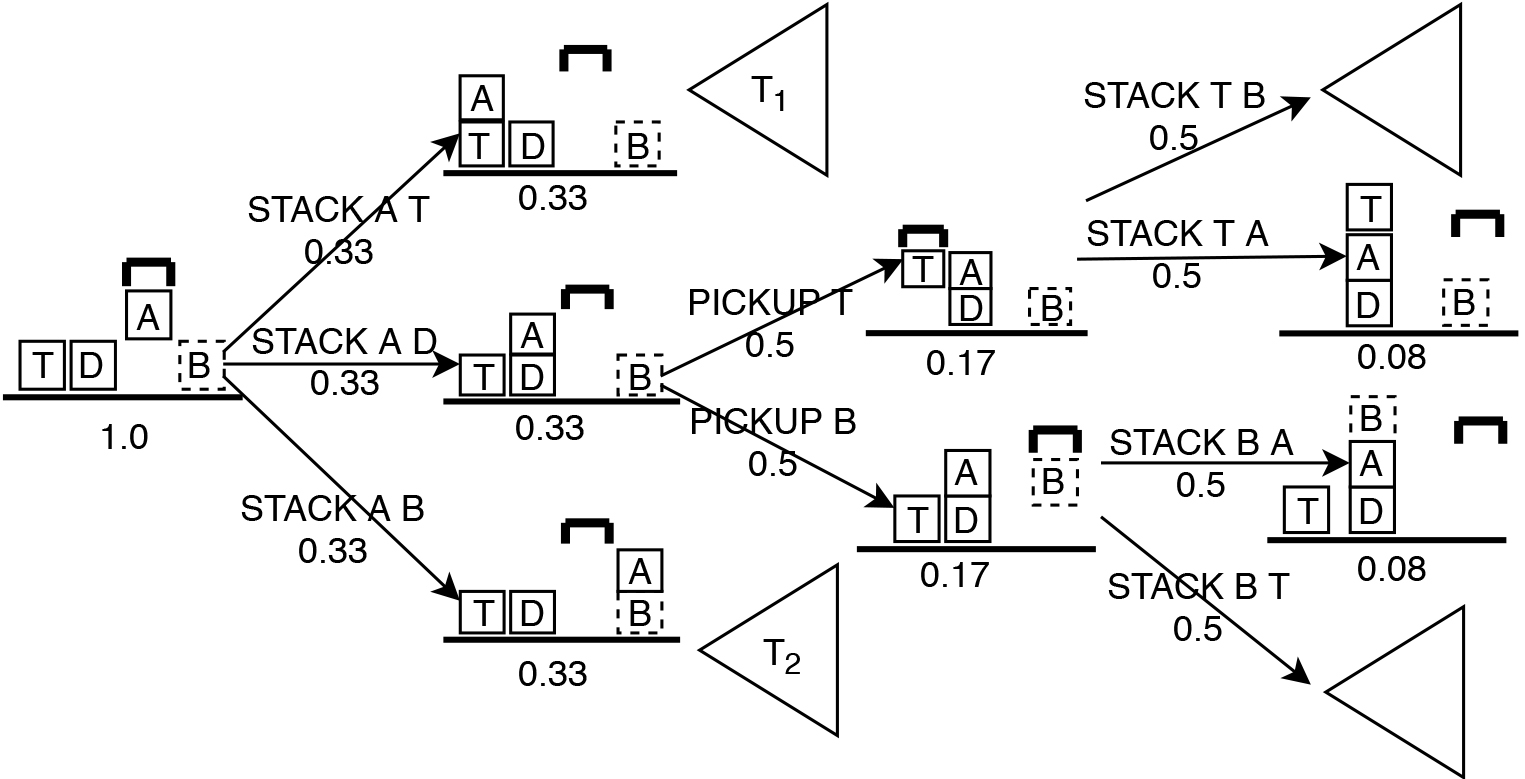
\includegraphics[width=0.6\columnwidth]{img/figure3.jpg}}
        \caption{Fragment of the decision space after PICKUP A has been proposed for block-words example in Figure \ref{fig:bw2} (B). Numbers under each state and action indicate the probability. Sub trees $T_1$ and $T_2$ are not expanded for simplicity.}
        \label{fig:feature}
\end{figure} 

\subsubsection{Risk ($R$)}
Risk quantifies the probability that the presented action will lead to \undesired.
$R$ is also coupled with the uncertainty the observer has about what the next action the user or the competitor (if present) will present. 
We model the uncertainty the observer has about the next action the user (or the competitor) presents as a uniform probability distribution across the set of applicable actions whose preconditions are satisfied in current state. 
We define $R$ as the posterior probability of reaching \undesired while the user is trying to achieve \desired. 
We extract \Suffixes from the Intervention Graph by searching breadth-first from the root until vertices containing \desired is found, including the paths in which the user has been subverted to reach \undesired. 
By construction, \desired will always be a leaf.
Let $\left | \Suffixes \right |=n$. 
The set of unsafe intervention suffixes, \SuffixesUnsafe is such that $\SuffixesUnsafe \subseteq \Suffixes$ and $\left | \SuffixesUnsafe \right |=m$ and $(m\leq n)$.
We compute posterior probability of reaching \undesired for \SuffixesUnsafe, using the chain rule in probability as, 
$Pr_{\textnormal{unsafe}}=\prod_{i=k}^{1}P(\alpha_i|\alpha_{i-1}\ldots \alpha_1)$, and $\alpha_{j} \in \lbrace\actionsTemplate{user}\rbrace$ or $\alpha_j\in\lbrace\actionsTemplate{user}\cup\actionsTemplate{other}\rbrace$ and $k$ is the length of the suffix until \undesired is reached. Then: 
\begin{equation*} 
R = \left\{\begin{matrix} \frac{\sum_{i=1}^{m}Pr_{\textnormal{unsafe}_i}}{m} & m>0\\ 0 &  m=0 \end{matrix}\right.
\end{equation*}
In Figure \ref{fig:feature}, $(n=6)$ and $(m=1)$. 
Since we assumed full observability for the observer, the root of the tree (current state) is assigned the probability of 1.0. 
Actions that are immediately possible after the current state are each assigned probabilities following a uniform distribution across the branching factor (0.33). 
Then for each applicable action in the current state, the resulting state gets the probability of ($1.0\times0.33=0.33$). 
Similarly, we apply the chain rule of probability for each following state and action level in the graph until \undesired first appears in the suffix. $R=\frac{0.08}{1}=0.08$.

\subsubsection{Desirability ($D$)}
Desirability measures the effect of the observed action to help the user pursue \desired safely.
\Suffixes is the same from $R$.
Let \SuffixesSafe be the set of suffixes that reach \desired while avoiding \undesired. Then $\SuffixesSafe =  \Suffixes\setminus\SuffixesUnsafe$.
We compute  posterior probability of reaching \desired avoiding \undesired for \SuffixesSafe, using the chain rule in probability as, $Pr_{safe}=\prod_{i=k}^{1}P(\alpha_i|\alpha_{i-1}\ldots \alpha_1)$, and $\alpha_{j} \in \lbrace\actionsTemplate{user}\rbrace$ or $\alpha_j\in\lbrace\actionsTemplate{user}\cup\actionsTemplate{other}\rbrace$ and $k$ is the length of path. Then:
\begin{equation*} 
D = \left\{\begin{matrix}
\frac{\sum_{i=1}^{|\SuffixesSafe|}Pr_{safe_i}}{|\SuffixesSafe|} & |\SuffixesSafe|>0\\ 
0 &  |\SuffixesSafe|=0
\end{matrix}\right.
\end{equation*} 
In Figure \ref{fig:feature}, there are five instances where user achieved \desired  without reaching \undesired (two in sub tree $T_1$, three in the expanded branch). Following the same approach to assign probabilities for states and actions, $D= \frac{(0.08+0.08+0.08+0.04+0.04)}{5} = 0.07$.
$R$ and $D$ are based on probabilities indicating the confidence the observer has about the next observation. 
We also use graph based distance measures: (1) distance to \undesired  ($\delta_\undesired$) and (2) distance to \desired ($\delta_\desired$). Both distances are measured in the number of edges in the paths from the root of the Intervention Graph to a state containing \desired or \undesired. 


\subsubsection{Distance to $\boldsymbol{\undesired}$ ($\delta_\undesired$)} 
This feature measures the distance to state \undesired from the current state in terms of the number of edges in the paths in \Suffixes extracted from the Intervention Graph. 
We extract \Suffixes from the Intervention Graph from the root to any vertex containing \desired, including the paths in which the user has been subverted to reach \undesired instead. 
Let $\left | \Suffixes \right |=n$. 
The set of suffixes that reach \undesired, \SuffixesUnsafe is such that $\SuffixesUnsafe \subseteq \Suffixes$ and $\left | \SuffixesUnsafe \right |=m$ and $(m\leq n)$.
We count  $s$, the number of the edges (actions) before \undesired is reached for each path in \SuffixesUnsafe and $\delta_\undesired$ is defined as the average of these distance values:
\begin{equation*} 
\delta_\undesired = \left\{\begin{matrix}
\frac{\sum_{i=1}^{m}s_i}{m} & m>0\\ 
-1 &  m=0
\end{matrix}\right.
\end{equation*} 
In this formula, $-1$ indicates that the undesirable state is not reachable from the current state. For the example problem illustrated in Figure \ref{fig:feature}, $\delta_\undesired=\frac{3}{1}=3$.

\subsubsection{Distance to $\boldsymbol{\desired}$ ($\delta_\desired$)} 
This feature measures the distance to \desired from current state. The path set \SuffixesSafe contains action sequences that reach \desired without reaching \undesired.
We count  $t$, the number of the edges where \desired is achieved safely for a path in \SuffixesSafe. 
Then, $\delta_\desired$ is defined as the average of these distances given by the formula:
\begin{equation*} 
\delta_\desired = \left\{\begin{matrix}
\frac{\sum_{i=1}^{|\SuffixesSafe|}t_i}{|\SuffixesSafe|} & |\SuffixesSafe|>0\\ 
-1 &  |\SuffixesSafe|=0
\end{matrix}\right.
\end{equation*}
In this formula, $-1$ indicates that \desired can not be reached safely from the current state. For the example problem illustrated in Figure \ref{fig:feature}, $\delta_\desired=\left \lceil \frac{3+3+7+7+3}{5} \right \rceil=5$.


\subsubsection{Active attack landmark percentage ($\mathcal{L}_{ac}$)} 
This feature captures the criticality of the current state toward contributing to \undesired. 
We used the algorithm proposed by Hoffmann et al. \citeyear{hoffman2004lm} to extract fact landmarks for the planning problem $P = \langle \domainTemplate{other}, \mathrm{u}\rangle$ or $P = \langle \domainTemplate{user}, \mathrm{u}\rangle$. 
These landmarks are referred to as \textit{attack landmarks} ($\mathcal{L}_{u}$) because they establish predicates that must be true to reach \undesired.  
Landmarks have been successfully used in deriving heuristics in Plan Recognition \cite{vered2018goalrec} and generating alternative plans \cite{bryce2014diverse}. 
We compute the percentage of active attack landmarks in the current state ($\mathcal{L}_{ac}$). 
To compute $\mathcal{L}_{ac}$ in Figure \ref{fig:feature}, we count the number of landmark predicates that have become active $(l)$ in the root of the Intervention Graph. 
Then, $\mathcal{L}_{ac}$ is given by the formula: $\mathcal{L}_{ac} = \frac{l}{\left |\mathcal{L}_{u}\right|}$. In Figure \ref{fig:feature}, $l=4$ and $\mathcal{L}_{ac}=4/10=0.4$.

For each presented action, the Intervention Graph is generated and features are computed, producing the corresponding feature vector. Landmarks for the problem are computed apriori.

\subsection{Plan Space Sampling and Plan Distance Metrics}
\label{sec:planspacesampling}
Extracting Intervention Graph features can be intractable when the graph is large, there are multiple paths reaching \desired, or multiple undesirable goals. 
Therefore, for our second method for implementing $plan(o_i,g)$ we define an additional set of features, called \textit{Sampled Features} by sampling the plan space for the observer.
If the Intervention Problem is defined for a single user, we sample the observer's plan space by using an automated planner to find solutions for $P_{\textnormal{observer}}=\langle \factsUser,\actionsUser, \initialState, g\rangle$, where $g\in\lbrace \desired,\undesired \rbrace$.
If the Intervention Problem is defined for a user and a competitor, we sample the observer's plan space by using an automated planner to find solutions for $P_{\textnormal{observer}}=\langle \factsOther,\actionsUser\cup\actionsOther, \initialState, g\rangle$, where $g\in\lbrace \desired,\undesired \rbrace$. 
Note that in this method we omit \dandu for generating plans.
Sampled plans are generated with the Top-K planner \cite{riabov2014}. 
We estimate the Risk and Desirability using plan distance metrics. The intuition is that if the actor is executing an unsafe plan, then that plan should be more similar to a sample of unsafe plans, compared to a sample of safe plans. 


For each presented action, the observer computes plan distances between a reference plan ($\pi^\prime$) and sampled plans ($\Pi^{\prime\prime}$) for both \undesired and \desired.
We follow the method proposed by Vered et al. \citeyear{vered2017} to generate the observation compatible plan by concatenating the observation history with the optimal plan that reaches \undesired (and \desired) to produce $\pi^\prime$.
 
We use the Top-K planner with K$=$50 to sample the plan space.
We use Action Set Distance (ASD), State Sequence Distance (SSD), Causal Link Distance (CLD) \cite{nguyen2012generating}, Generalized Edit Distance (GED) for sequences of states and actions \cite{sohrabi2016finding} to measure the distances between the reference plan and the sampled plans for \desired and \undesired. When an action is presented, $\pi^\prime$ is computed. 
Then, observation compatible Top-K plans are produced for \undesired and \desired separately. 
Then we compute the medians of ASD, CLD and SSD, minimum remaining actions to \undesired and \desired, minimum action GED and state GED are computed for \undesired and \desired for all $\langle$reference, sample$\rangle$ pairs. 
This produces the Sampled Feature vector for the presented action. Algorithm~\ref{alg:apx} shows the pseudo-code for computing the Sampled Feature vector.

\begin{algorithm}[ht]
%\scriptsize
        \caption{Build Sampled Feature Vector}
        \label{alg:apx}
        \begin{algorithmic}[1]
                \Require $D$, $s$, \undesired, \desired
                \State $i=0;$ $ s_{i} \gets \initialState$
                \State $prefix,suffix,\Pi^{\prime\prime}, \mathcal{V} \gets \varnothing$
                \Procedure{sampledsuffixes}{$D_1,s,\mathrm{u},\mathrm{d},O$}
                        %\State $\mathcal{L}_{u} \gets$ compute remaining landmarks for the problem $P_1\langle D_1, \mathrm{u}\rangle$
                \For{$o \in O$}
                        \State \parbox[t]{0.95\linewidth}{$prefix \gets prefix + o$}
                        \State \parbox[t]{0.95\linewidth} 
                                {$s_{i+1} \gets ((s_{i} \setminus Del(o))\cup Add(o))$}
                        \For {$ g \in \{\mathrm{u}, \mathrm{d}$\}}
                                \State \parbox[t]{0.95\linewidth}{$suffix \gets OptimalPlan(s,g)$}
                                \State \parbox[t]{0.95\linewidth}{$\pi^\prime \gets prefix + suffix$}
                                \State \parbox[t]{0.95\linewidth}{$\Pi^{\prime\prime} \gets \text{Observation compatible Top-K plans for } g$}
                                \State \parbox[t]{0.95\linewidth}{$v_1 \gets$ MedianActionSetDist$(\pi^\prime, \Pi^{\prime\prime})$}
                                \State \parbox[t]{0.95\linewidth}{$v_2 \gets$ MedianCausalLinkDist$(\pi^\prime, \Pi^{\prime\prime})$}
                                \State \parbox[t]{0.95\linewidth}{$v_3 \gets$ MedianStateSequenceDist$(\pi^\prime,\Pi^{\prime\prime})$}
                                \State \parbox[t]{0.95\linewidth}{$v_4 \gets$ MinimumRemainingDistToState $(g,\Pi^{\prime\prime})$}
                                \State \parbox[t]{0.95\linewidth}{$v_5 \gets$ MinimumActionGED $(\pi^\prime, \Pi^{\prime\prime})$}
                                \State \parbox[t]{0.95\linewidth}{$v_6 \gets$ MinimumStateGED $(\pi^\prime, \Pi^{\prime\prime})$}
                                \State $\mathcal{V}(o) \gets \lbrack v_1,v_2,v_3,v_4,v_5,v_6\rbrack $
                        \EndFor
                        %\State \parbox[t]{0.95\linewidth}{$v_7 \gets$ AchievedLandmarkHeuristic $(\mathrm{u},s_{i})$}
                        %\State $\mathcal{V}(o) \gets \mathcal{V}(o)+\{v_7\}$
                \EndFor
                \EndProcedure
        \end{algorithmic}
\end{algorithm}

\subsection{Learning When to Intervene}
\label{sec:learning-to-intervene}
We train a classifier to categorize the presented observation $o_i$ into two classes: (Yes) indicating intervention is required and (No), indicating otherwise. 
We chose Naive Bayes, K-nearest neighbors, decision tree and logistic regression classifiers from Weka~\footnote{\url{http://www.cs.waikato.ac.nz/ml/weka/}}. 
Given a observations labeled as Yes/No and corresponding feature vectors as training examples, we train the classifiers with 10-fold cross validation. 
The trained model is used to predict intervention for previously unseen Intervention Problems. 
Attribute selected classifiers filter the feature vector to only select critical features. 
This step reduces complexity of the model, makes the outcome of the model easier to interpret, and reduces over-fitting. 

We generated training data from twenty Intervention Problems using the benchmark domains. We used the Blocks World domain to model competitive Intervention Problems and Ferry, EasyIPC and Navigator domains to model Standard Intervention Problems.
We restricted the number of observation traces per Intervention Problem to 100 for training the classifiers.
 
A full parameter search revealed the best parameters for the classifiers. 
The decision tree classifier is tuned to pruning confidence=0.25 and minimum number of instance per leaf=2. 
The K-nearest neighbor classifier is tuned to use k=1 and distance measure=Euclidean. 
The logistic regression classifier is tuned for ridge parameter = 1.0E-8. 
The Naive Bayes classifier is tuned with the supervised discretization=True.
%
%%%%===========================================================================================================
%%%%===========================================================================================================
\section{Evaluating Intervention Recognition}
\label{sec:evaluating-intervention}
We now discuss the accuracy of the intervention recognition solutions.
As the baseline, we compare the learning based intervention accuracy to three state-of-the-art Plan Recognition algorithms from the literature. 
Our evaluation focuses on two questions: (1) Using domain-independent features indicative of the likelihood to reach \undesired from current state, can the observer correctly recognize directly and indirectly contributing suffixes to prevent the user from reaching \undesired? and (2) How does the learning approach perform against state-of the-art Plan Recognition? 
To address the first question, we evaluated the performance of the learned model on unseen Intervention Problems.

The benchmarks consist of Blocks-words, IPC Grid, Navigator and Ferry domains. For the \textbf{Blocks-words} domain, we chose word building problems. The user and the competitor want to build different words with some common letters. 
The problems in \textbf{Blocks-1} model intervention by identifying the direct contributors ($a_{crit}$), whereas the problems in \textbf{Blocks-2} model intervention by identifying the indirect contributors ($q_{crit}$) in the Blocks-words domain.
In the \textbf{IPC grid} domain, the user moves through a grid to get from point A to B. 
Certain locked positions on the grid can be opened by picking up keys. In the \textbf{Navigator} domain, the user moves from one point on a grid to another. In IPC Grid and Navigator domains, we designated certain locations on the grid as traps. The goal of the user is to navigate to a specific point on the grid without passing through the trap. In the \textbf{Ferry} domain, a single ferry moves cars between different locations. We assigned a port as \emph{compromised}. The ferry's objective is to transport cars to specified locations without passing the compromised port. 


To evaluate our trained classifiers, we generate 3 separate test problems of 20 instances each (total of 60) 
for the benchmark domains with problems different from training instances. 
The three test instances differ from the number of blocks in the Blocks Words domain, size of grid (Navigator, IPC-Grid), accessible and inaccessible paths on the grid (Navigator, IPC-Grid), and properties of artifacts in the grid (IPC-Grid). 
For each test instance we generated 10 observation traces (total of 600 test observation traces). 


We define true-positive as the classifier correctly identifying the presented action to be in $a_{crit}$ or $q_{crit}$. 
True-negative is an instance where the classifier  correctly identifying an action as not belonging to $a_{crit}$ or $q_{crit}$. False-positives are instances where classifier incorrectly identifies an action as belonging to $a_{crit}$ or $q_{crit}$. False-negatives are instances where the classifier incorrectly identifies the presented action as not belonging to $a_{crit}$ or $q_{crit}$. 
Naturally, our test observation traces contain a large number of negatives. 
To offset the bias introduced to the classifier by the class imbalance, we report Matthews correlation coefficient (MCC) because it gives an accurate measure of the quality of a binary classification while taking into account the different class sizes.
 We also report the F-score $= \frac{tp}{tp+1/2(fp+fn)}$ for the classifiers. $tp$, $fp$, $fn$ are the number of true positives, false positives and false negatives respectively.

\begin{table}[ptb]
\resizebox{\textwidth}{!}{%
\begin{tabular}{|l|ll|ll|ll|ll|ll|l|l}
\hline
\multicolumn{1}{|c|}{\multirow{3}{*}{Domain}} & \multicolumn{6}{c|}{Naive Bayes} & \multicolumn{6}{c|}{Decision Tree} \\ \cline{2-13} 
\multicolumn{1}{|c|}{} & \multicolumn{2}{c|}{Instance 1} & \multicolumn{2}{c|}{Instance 2} & \multicolumn{2}{c|}{Instance 3} & \multicolumn{2}{c|}{Instance 1} & \multicolumn{2}{c|}{Instance 2} & \multicolumn{2}{c|}{Instance 3} \\ \cline{2-13} 
\multicolumn{1}{|c|}{} & \multicolumn{1}{l|}{F-score} & \multicolumn{1}{c|}{MCC} & \multicolumn{1}{c|}{F-score} & MCC & \multicolumn{1}{l|}{F-score} & MCC & \multicolumn{1}{l|}{F-score} & MCC & \multicolumn{1}{l|}{F-score} & MCC & F-score & \multicolumn{1}{l|}{MCC} \\ \hline
\multicolumn{13}{|c|}{Intervention Graph Method} \\ \hline
\textbf{Blocks-1} & 1 & 1 & 1 & 1 & 1 & 1 & 1 & 1 & 1 & 1 & 1 & \multicolumn{1}{l|}{1} \\ \cline{1-1}


\textbf{Blocks-2} & 1 & 1 & 1 & 1 & 1 & 1 & 1 & 1 & 1 & 1 & 1 & \multicolumn{1}{l|}{1} \\ \cline{1-1}


\textbf{EasyIPC} & 1 & 1 & 1 & 1 & 1 & 1 & 1 & 1 & 1 & 1 & 1 & \multicolumn{1}{l|}{1} \\ \cline{1-1}
\textbf{Ferry} & 1 & 1 & 1 & 1 & 1 & 1 & 1 & 1 & 1 & 1 & 1 & \multicolumn{1}{l|}{1} \\ \cline{1-1}
\textbf{Navigator} & 1 & 1 & 1 & 1 & .99 & .99 & .87 & .87 & .72 & .74 & .90 & \multicolumn{1}{l|}{.90} \\ \hline


\multicolumn{13}{|c|}{Plan Space Sampling Method} \\ \hline
\textbf{Blocks-1} & .25 & .33 & .25 & .33 & .25 & .33 & .25 & .33 & .25 & .33 & .25 & \multicolumn{1}{l|}{.33} \\ \cline{1-1}
\textbf{Blocks-2} & 1 & 1 & 1 & 1 & 1 & 1 & 1 & 1 & 0.99 & 0.99 & 1 & \multicolumn{1}{l|}{1} \\ \cline{1-1}


\textbf{EasyIPC} & 1 & 1 & 1 & 1 & 1 & 1 & 1 & 1 & 1 & 1 & 1 & \multicolumn{1}{l|}{1} \\ \cline{1-1}
\textbf{Ferry} & .34 & .33 & .32 & .31 & 0.02 & -.004 & .25 & .28 & .24 & .23 & .86 & \multicolumn{1}{l|}{.86} \\ \cline{1-1}
\textbf{Navigator} & 1 & 1 & 1 & 1 & 1 & 1 & .62 & .65 & 1 & 1 & 1 & \multicolumn{1}{l|}{1} \\ \hline
\end{tabular}%
}
\caption{F-score and MCC for predicting intervention using  Intervention Graph and plan space sampling methods for Naive Bayes and Decision Tree classifiers}
\label{tab:exactapprox1}
\end{table}


\begin{table}[ptb]
\resizebox{\textwidth}{!}{%
\begin{tabular}{|l|ll|ll|ll|ll|ll|ll|}
\hline
\multicolumn{1}{|c|}{\multirow{3}{*}{Domain}} & \multicolumn{6}{c|}{Logistic Regression} & \multicolumn{6}{c|}{K-Nearest} \\ \cline{2-13} 
\multicolumn{1}{|c|}{} & \multicolumn{2}{c|}{Instance 1} & \multicolumn{2}{c|}{Instance 2} & \multicolumn{2}{c|}{Instance 3} & \multicolumn{2}{c|}{Instance 1} & \multicolumn{2}{c|}{Instance 2} & \multicolumn{2}{c|}{Instance 3} \\ \cline{2-13} 
\multicolumn{1}{|c|}{} & \multicolumn{1}{l|}{F-score} & MCC & \multicolumn{1}{l|}{F-score} & MCC & \multicolumn{1}{l|}{F-score} & MCC & \multicolumn{1}{l|}{F-score} & MCC & \multicolumn{1}{l|}{F-score} & MCC & \multicolumn{1}{l|}{F-score} & MCC \\ \hline
\multicolumn{13}{|c|}{Intervention Graph Method} \\ \hline
\textbf{Blocks-1} & 1 & 1 & 1 & 1 & 1 & 1 & 1 & 1 & 1 & 1 & 1 & 1 \\ \cline{1-1}
\textbf{Blocks-2} & 1 & 1 & 1 & 1 & 1 & 1 & 1 & 1 & 1 & 1 & 1 & 1 \\ \cline{1-1}
\textbf{EasyIPC} & .88 & .87 & .88 & .87 & .86 & .86 & 1 & 1 & 1 & 1 & 1 & 1 \\ \cline{1-1}
\textbf{Ferry} & 1 & 1 & 1 & 1 & 1 & 1 & 1 & 1 & 1 & 1 & 1 & 1 \\ \cline{1-1}
\textbf{Navigator} & 1 & 1 & 1 & 1 & .99 & .99 & 1 & 1 & .96 & .96 & .99 & .99 \\ \hline

\multicolumn{13}{|c|}{Plan Space Sampling Method} \\ \hline
\textbf{Blocks-1} & .25 & .33 & .25 & .33 & .25 & .33 & 1 & 1 & 1 & 1 & 1 & 1 \\ \cline{1-1}
\textbf{Blocks-2} & 1 & 1 & 1 & 1 & 1 & 1 & 1 & 1 & 1 & 1 & 1 & 1 \\ \cline{1-1}

\textbf{EasyIPC} & .64 & .63 & .46 & .44 & .67 & .66 & .05 & -.04 & .04 & -.03 & .05 & -.02 \\ \cline{1-1}
\textbf{Ferry} & .31 & .32 & .23 & .22 & 1 & 1 & .33 & .40 & .13 & .15 & .81 & .82 \\ \cline{1-1}
\textbf{Navigator} & .60 & .59 & .98 & .94 & .97 & .97 & .61 & .65 & 1 & 1 & 1 & 1 \\ \hline
\end{tabular}%
}
\caption{F-score and MCC for predicting intervention using  Intervention Graph and plan space sampling methods for logistic regression and k-nearest neighbor classifiers}
\label{tab:exactapprox2}
\end{table}

\begin{table}[ptb]
\resizebox{\textwidth}{!}{%
\begin{tabular}{|l|ll|ll|ll|ll|ll|ll|ll|ll|ll|}
\hline
\multicolumn{1}{|c|}{\multirow{3}{*}{Domain}} & \multicolumn{6}{c|}{Instance 1} & \multicolumn{6}{c|}{Instance 2} & \multicolumn{6}{c|}{Instance 3} \\ \cline{2-19} 
\multicolumn{1}{|c|}{} & \multicolumn{2}{c|}{RG (LAMA)} & \multicolumn{2}{c|}{RG (HSP)} & \multicolumn{2}{c|}{GM} & \multicolumn{2}{c|}{RG (LAMA)} & \multicolumn{2}{c|}{RG (HSP)} & \multicolumn{2}{c|}{GM} & \multicolumn{2}{c|}{RG (LAMA)} & \multicolumn{2}{c|}{RG (HSP)} & \multicolumn{2}{c|}{GM} \\ \cline{2-19} 
\multicolumn{1}{|c|}{} & \multicolumn{1}{l|}{F-score} & MCC & \multicolumn{1}{l|}{F-score} & MCC & \multicolumn{1}{l|}{F-score} & MCC & \multicolumn{1}{l|}{F-score} & MCC & \multicolumn{1}{l|}{F-score} & MCC & \multicolumn{1}{l|}{F-score} & MCC & \multicolumn{1}{l|}{F-score} & MCC & \multicolumn{1}{l|}{F-score} & MCC & \multicolumn{1}{l|}{F-score} & MCC \\ \hline
\textbf{Blocks-1} & .38 & .45 & .38 & .45 & .36 & .43 & .43 & .49 & .43 & .49 & .39 & .45 & .40 & .47 & .40 & .47 & .38 & .45 \\ \cline{1-1}
\textbf{Blocks-2} & 1 & 1 & .90 & .90 & 1 & 1 & 1 & 1 & .90 & .90 & 1 & 1 & 1 & 1 & .90 & .90 & 1 & 1 \\ \cline{1-1}
\textbf{EasyIPC} & .13 & .05 & .13 & .05 & .10 & .01 & .21 & .17 & .18 & .13 & .12 & .06 & .23 & .19 & .22 & .19 & .14 & .09 \\ \cline{1-1}
\textbf{Ferry} & .17 & .18 & .22 & .20 & .10 & .08 & .23 & .22 & .11 & .06 & .15 & .09 & .15 & .17 & .47 & .52 & .21 & .34 \\ \hline
\end{tabular}%
}
\caption{F-score and Matthews Correlation Coefficient (MCC) for recognizing intervention with probabilistic goal recognition (RG) using a satisficing (LAMA) and optimal (HSP) planners goal mirroring (GM). For the Navigator domain Intervention Problems, the true-negative, false negative rates were 100\%  each. Therefore, F-score and MCC are not reported for that problem set.}
\label{tab:rgv}
\end{table}




We implemented three state-of-the art Plan Recognition algorithms to compare the accuracy of intervening by Plan Recognition to the proposed learning based intervention. 
We selected Ramirez and Geffener's probabilistic Plan Recognition algorithm \cite{ramirez2010probabilistic} (both the satisficing, and optimal implementations) and the Goal Recognition with Goal Mirroring algorithm \cite{vered2018goalrec}. 
To generate satisficing plans we used the Fast Downward planner with the FF heuristic and context-enhanced additive heuristic \cite{helmert2006}.
To generate the optimal cost plans we used the HSP planner \cite{bonet01planningas}.
For each presented action, the observer solves a Plan Recognition problem using each approach. 
We assumed uniform priors for over \undesired and \desired. 
If \undesired is the top ranked goal for the presented action, then it is flagged as requiring intervention. 
The assumption is that these algorithms must also be able to correctly identify \undesired as the most likely goal for the actions in $a_{crit}$ and $q_{crit}$. 
We used the same test data suite to evaluate accuracy.

Tables \ref{tab:exactapprox1} and ~\ref{tab:exactapprox2} shows that the classifiers trained with features from the Intervention Graph achieve high accuracy for all the domains when predicting intervention for both identifying actions in $a_{crit}$ and $q_{crit}$. 
The MCC value shows that the imbalance in class sizes does not bias the classifier. 
Low false positives and false negatives suggests that the user will not be unnecessarily interrupted. 
As expected performance degrades when we use a sampled plan space to derive features.
However, the features derived from sampling the plan space produce equally good classifiers compared to the intervention graph method, when  modeling intervention by identifying actions in $a_{crit}$ and $q_{crit}$  for the Blocks-word problems.
For the Intervention Problems modeled using the benchmark domains, we were able to find that at least one of the selected classifiers responded with very high F-score when trained using plan similarity features. 
The exception to this pattern was the Intervention Problems modeled using the Ferry domain.

Features derived from the Intervention Graph accurately recognize actions in $a_{crit}$ and $q_{crit}$ where the user has limited options available to reach the desirable goal while avoiding the undesirable state. 
Thus the classifiers perform well in recognizing critical actions in new problems. 
The sampled features rely on the learning algorithm to produce accurate results when predicting intervention. 

Comparing the results in Table \ref{tab:rgv}, learning methods outperform existing Plan Recognition algorithms when predicting intervention. 
The algorithms we selected clearly struggled to predict intervention in the Navigator domain producing many false positives and false negatives.
These results suggest that although we can adopt existing Plan Recognition algorithms to identify when the user needs intervention, it also produces a lot of false negatives and false positives in correctly identifying which state (desirable/undesirable) is most likely given the observations, especially when the desirable and undesirable plans have a lot of overlap.
Comparing recognition accuracy of Blocks-1 and Blocks-2 problems using plan recognition algorithms to intervene, we see that when the undesirable state develops over a long period of time, the plan recognition algorithms recognize the undesirable plan with high accuracy. 
In other words, if the \desired and \undesired are sufficiently distinct and are far apart in the state space, intervention by using plan recognition algorithms are as effective as our proposed learning based intervention methods in most cases.
When the desirable and undesirable states are closer, existing plan recognition algorithms produce many false positives/negatives.
This is unhelpful specially considering human users because, when the intervening agent produces may false alarms and/or miss critical events that should be intervened the human users may get frustrated and turn off intervention.
Therefore, the learning approach is better suited for intervention because the observer can target specific critical actions  and at the same time the user is given some freedom to pursue his own desirable goal.

%%%===========================================================================================================
%
%%%=====================================================================================
\section{Human-Aware Intervention}
\label{sec:human-aware}
The Human-aware Intervention Problem is a variant of the single-user intervention, so the history \historyDef consists of only accepted user actions.
However, as mentioned in Section~\ref{sec:models}, the set of projections will be empty, that is $\Suffixes = \emptyset$ because planning is less accurate for projecting what the human user may do.
This means the observer must emphasize analysis of \historyDef.
Instead of relying on projections in \Suffixes, the observer \emph{learns} the function $intervene_i$.
That is, at the presented action $o_i$ it considers only $H$, \desired, and \undesired and uses a trained machine learning algorithm to decide whether to intervene.

We introduce the Rush Hour puzzle as a benchmark in order to study how human users solve the puzzle as a planning task that require intervention.
We begin with the formal definitions of the Rush Hour puzzle.
Next, we translate the Rush Hour problem into a STRIPS planning task and through a human subject study, we allow human users solve the planning problem and collect observation traces.
We formally define the Human-aware Intervention problem and propose a solution that uses machine learning to learn properties of \historyDef to determine whether or not intervention is required.
The observer for Human-aware Intervention should offer different levels of freedom to the user.
At the lowest level of freedom, the observer will intervene just before the undesirable state. 
At increased levels of freedom, the observer offers the user enough time to recover from the undesirable situation.
Varying the level of freedom allows the observer to gradually guide the user toward \desired without directly giving away the complete solution.
We evaluate the accuracy of our learning approach using the observation traces collected from the human subject study.


 

\subsection{The Rush Hour Puzzle}
The Rush Hour puzzle is a game for ages 8 and above. Figure \ref{fig:game}A shows an initial puzzle configuration on a $6 \times 6$ grid, where cars (length 2) and trucks (length 3) are arranged. 
Vertically aligned vehicles can only move up and down and horizontal vehicles can move left and right. 
Vehicles can be moved one at a time and into adjacent empty spaces. The solution to the Rush Hour puzzle is a sequence of legal moves that transforms the initial board state shown in \ref{fig:game}A to the goal state in \ref{fig:game}B. 
For the puzzle shown in Figure \ref{fig:game}, the shortest solution has 21 moves, if the number of moves is considered as the optimizing criteria. 
If optimized for the number of vehicles moved, the puzzle can be solved optimally by moving only 8 vehicles. 
It is important to note that one can obtain different ``optimal solutions" depending on whether the number of moves is minimized,
or if the number of vehicles moved is minimized.
Humans tend not to clearly make this distinction when playing the game.
\begin{figure}[tpb]
  \centering
    	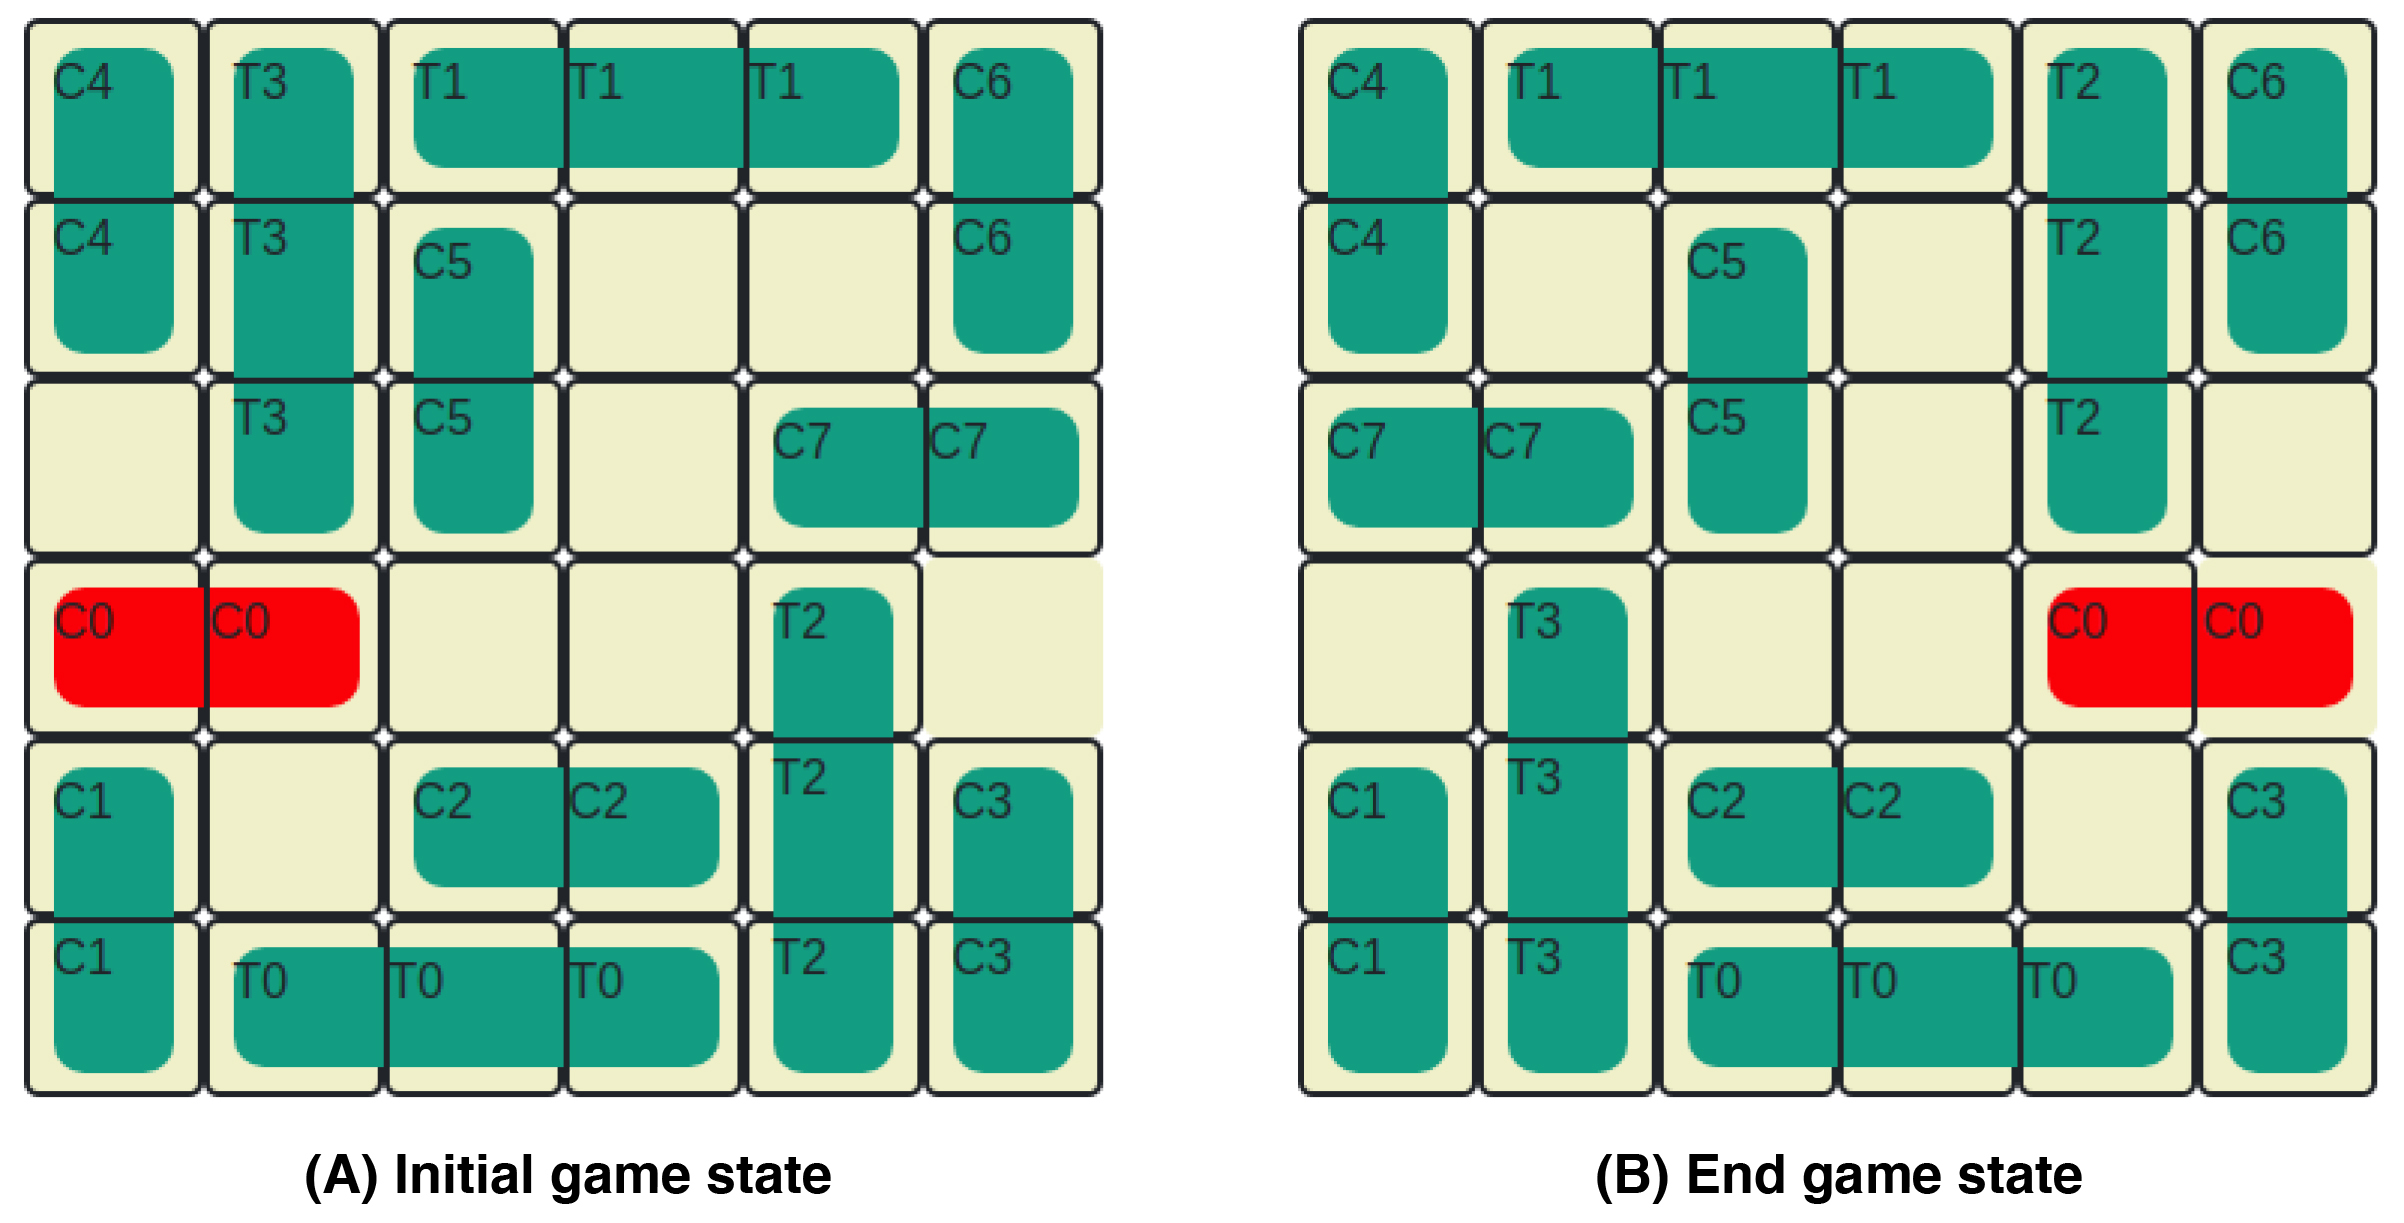
\includegraphics[width=0.7\textwidth]{img/figure4.jpg}
    	\caption{A Rush Hour instance}
    	\label{fig:game}
\end{figure}

We adopt the formal definition of a Rush Hour instance from Flake et al. \citeyear{flake2002}. 

\begin{definition} 
\label{def:rush}
A \textnormal{Rush Hour instance} is a tuple $\langle w,h,x,y,n,\mathcal{V}\rangle$ such that:
\begin{itemize}
\item $(w,h) \in {\mathbb{N}}^2$ are the grid dimensions. In the standard version, $w=h=6$
\item $(x,y), x\in\lbrace 1,w\rbrace$ and $y\in\lbrace 1,h\rbrace$ are the coordinates of the exit, which must be on the grid perimeter.
\item $n \in \mathbb{N}$ the number of non-target vehicles
\item $\mathcal{V}=\lbrace v_0, \ldots, v_n \rbrace$ is the set of $n+1$ vehicles comprised of cars $(\mathcal{C})$ and trucks $(\mathcal{T})$. Note that $|\mathcal{V}|=|\mathcal{C}|+|\mathcal{T}|$
\\$v_i \in \mathcal{C}$ is identified as $\lbrace C_0,\ldots,C_l \rbrace$, where $l=|\mathcal{C}|-1$ and $v_i \in \mathcal{T}$ is identified as $\lbrace T_0,\ldots,T_m \rbrace$, where $m=|\mathcal{T}|-1$.
\\A vehicle is a tuple $v_i=\langle x_i,y_i,o_i,s_i \rangle$, where $(x_i,y_i) \in {\mathbb{N}}^2$ are the vehicle coordinates, $o_i \in \lbrace N,E,S,W\rbrace$ is the vehicle orientation for North, East, South, West, $s_i \in \lbrace2,3\rbrace$ is the vehicle size and $C_0$ is the target vehicle.
\end{itemize}
\label{rushdef}
\end{definition}
Flake et al. \citeyear{flake2002} also defines the \textit{solution} to a Rush Hour instance as a sequence of $m$ moves, where each move consists of a vehicle identifier $i$, a direction that is consistent with the initial orientation of $v_i$, and a distance. 
Each move, in sequence must be consistent with itself and with the configuration prior to the move. 
Further, in order to move a distance $d$ the configuration must be consistent for all $d^\prime$ such that, $0\leqslant d^\prime \leqslant d$ (i.e., a vehicle can not jump over other vehicles on its path).


\subsection{The Rush Hour Puzzle as a STRIPS Planning Task for Intervention}
\label{sec:rushhourstrips}
We study how human users approach solving a cognitively engaging problem as a planning task and evaluate whether we can use domain-specific features to predict intervention. 
To collect realistic data, it is critical that the human users were willing to participate in the task. 
The Rush Hour puzzle addresses this requirement well, as evidenced by the feedback about the task we received from the demographic survey. See Section~\ref{ap:demographics} in the Appendix for details.
Although, the puzzle is a game, the environment is rich enough to simulate undesirable consequences and also offer the users a task that is challenging enough.

We translate the Rush Hour puzzle in Definition~\ref{def:rush} into a grounded STRIPS planning task $P=\langle F, A, \initialState, G\rangle$ as follows:
\begin{itemize}
\item $F=\lbrace$ 
$\lbrace \forall C_i \in \mathcal{C}$, (\texttt{car} \texttt{?}$C_i$)$\rbrace$, 
$\lbrace \forall T_i \in \mathcal{T}$, (\texttt{truck} \texttt{?}$T_i$)$\rbrace$  - for the vehicles,\\
$\lbrace \forall v_i \in \mathcal{C}\cup \mathcal{T}$ and $l_i\in \lbrace(x,y)|x\in \left[ 1..w\right ], y \in \left[ 1..h\right] \rbrace$, (\texttt{at} \texttt{?}$v_i$ \texttt{?}$l_i$)$\rbrace$ - for the vehicle positions,\\
$\lbrace \forall v_i \in \mathcal{C}\cup \mathcal{T}$ and $d_i\in \lbrace NS, SN, EW, WE \rbrace$, (\texttt{face} \texttt{?}$v_i$ \texttt{?}$d_i$)$\rbrace$ - for direction of vehicles (North to South (down), South to North (up), East to West (left), West to East (right) respectively),\\
$\lbrace \forall l_i\in \lbrace(x,y)|x\in \left[ 1..w\right ], y \in \left[ 1..h\right]\rbrace$, (\texttt{free} \texttt{?}$l_i$)$\rbrace$ - for open positions,\\
$\lbrace \forall l_i, l_j\in \lbrace(x,y)|x\in \left[ 1..w\right ], y \in \left[ 1..h\right]\rbrace$ and $d_i\in \lbrace NS, SN, EW, WE \rbrace$, (\texttt{next} \texttt{?}$d_i$ \texttt{?}$l_i$ \texttt{?}$l_j$)$\rbrace$ - for direction of the adjacent locations)
$\rbrace$

\item $A = \lbrace$\texttt{move-car} = $\langle$pre(\texttt{move-car}), add(\texttt{move-car}), del(\texttt{move-car})$\rangle \subseteq F$, \\
\texttt{move-truck} = $\langle$pre(\texttt{move-truck}), add(\texttt{move-truck}), del(\texttt{move-truck})$\rangle \subseteq F  \rbrace$
\item $\initialState \subseteq F$
\item $G = \lbrace$(\texttt{at} $C_0$ $l_i$)(\texttt{at} $C_0$ $l_j$)$\rbrace$, where $l_i=(w,3)$ and $l_j=(w-1,3)$
\end{itemize}


In order to configure the Rush Hour STRIPS planning task for intervention, we introduce an undesirable state, \undesired by designating one vehicle as \textit{forbidden}. 
The post-conditions of any action that moves the forbidden vehicle satisfies \undesired. 
The puzzle can be solved without moving the forbidden vehicle.
Therefore, moving the forbidden vehicle is also an unnecessary action, indicating that the user is exploring an unhelpful region in the state space.
Here, intervention is required to guide the user toward exploring more helpful regions in the state space.
In the Figure~\ref{fig:game}A, the forbidden vehicle is $C_2$. If the user moves $C_2$ to the left, then the board state satisfies \undesired.
The user's goal $\desired = G$.
The vehicle movement constraint introduced by the presence of the forbidden vehicle adds an extra level of difficulty to the user's planning task. 

The Rush Hour problem is also unique in that the observer is more focused on states than actions.
Recall that a history  $\historyDef = ( o_1 [s_1], o_2 [s_2], \ldots, o_{i-1} [\historyEndState])$  is a sequence of previously observed actions, which started from \initialState with the implied resulting states in brackets.
For Rush Hour, the observer relies on those implied states instead of just the actions.
For simplicity in notation, we present intervention in terms of states, although it is easy to map between actions and states because of the deterministic state transition system of the planning model.


\subsection{Domain-Specific Feature Set}
For the observer to learn $intervene_i$, we develop a set of domain-specific features for the Rush Hour problem.
We want the feature set to capture whether the user is advancing toward \desired by making helpful moves, or whether the user currently exploring a risky part in the state space and getting closer to \undesired.
We hypothesize that the behavior patterns extracted from \historyDef as features have a correlation to the event of the user moving the forbidden vehicle. 

\subsubsection{Features Based on State}
The features based on state analyze the properties of the sequence of state transitions in \historyDef from \initialState to \historyEndState $( [\initialState], [s_1], [s_2], \ldots, [\historyEndState])$.
Specifically, we look at the \textit{mobility} of the objects: target vehicle ($C_0$), the forbidden vehicle and the vehicles adjacent to the target and the forbidden vehicles.
We use the state features associated with the target vehicle to measure how close the user is to \desired. 
The state features associated with the forbidden car evaluate how close the user is to triggering \undesired. 

We manually examined the solutions produced in the human subject experiment (described later) to identify common movement patterns. 
Our analysis revealed that if the user was moving vehicles adjacent to the forbidden vehicle in such a way that the forbidden vehicle was freed, most users ended up moving the forbidden vehicle. 
Therefore, by monitoring the state changes occurring around the forbidden vehicle, we can estimate whether the user will end up moving the forbidden vehicle or not (i.e., trigger \undesired). 
Similarly, state changes occurring on the target car’s path to the exit, for example, the moves that result in reducing the number of vehicles blocking the target car is considered to be helpful to move the state closer to \desired.

\begin{figure}[tpb]
  \centering
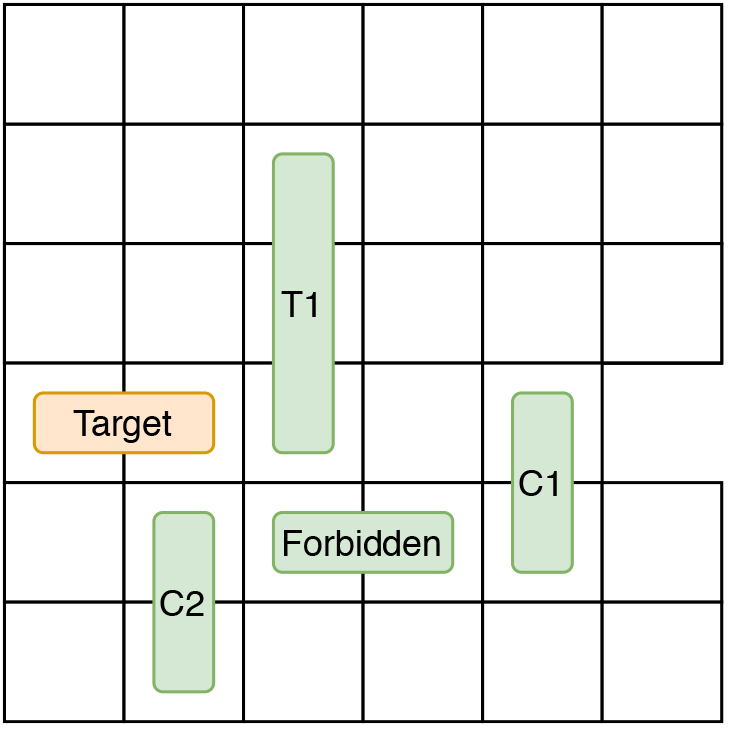
\includegraphics[width=0.25\columnwidth]{img/figure5.jpg}
  \caption{Blocker vehicles}
  \label{fig:blockers}
\end{figure}
We refer to the vehicles adjacent to the target and the forbidden vehicles as \textit{blockers} and introduce two additional object types to monitor mobility: \textit{target car blockers} and \textit{forbidden car blockers}. 
Figure~\ref{fig:blockers} illustrates an example state. 
The target car’s path is blocked by two vehicles $C_1$ and $T_1$. Therefore, target car blockers $=\lbrace C_1, T_1\rbrace$. 
We only consider the vehicles that are between the target car and the exit cell as target car blockers because, only those vehicles are preventing the target car from reaching \desired. 
The forbidden vehicle’s movement is blocked by two vehicles $C_1$ and $C_2$. 
Therefore, forbidden car blockers $=\lbrace C_1, C_2\rbrace$. 
We now describe the features based on state that are used to predict intervention in Human-aware Intervention Problems.

\begin{itemize}
\item \texttt{blocks}: number of times a move increased the number of cars blocking the target car's path
\item \texttt{frees}: number of times a move freed up empty spaces around the forbidden vehicle
\item \texttt{freebci}: number of times the number of empty spaces around the forbidden vehicle blockers increased
\item \texttt{freebcd}: number of times the number of empty spaces around the forbidden vehicle blockers decreased
\item \texttt{freegci}: number of times the number of empty spaces around the target car blockers increased
\item \texttt{freegcd}: number of times the number of empty spaces around around the target car blockers decreased
\item \texttt{mgc}: mean number of empty spaces around the target car blockers
\item \texttt{mbc}: mean number of empty spaces around the forbidden car blockers
\item \texttt{reset}: number of times the current move changed the state back to the initial puzzle configuration\\
\end{itemize}



\subsubsection{Features Based on User Actions}
The features based on user state analyze the properties of the sequence of actions from $o_1$ to $o_{i-1}$ in \historyDef $( o_1, o_2, \ldots, o_{i-1} )$
We follow the same manual analysis of solutions produced in the human subject experiment to identify common movement patterns. 
We found that the users who produce unsafe solutions often made unhelpful moves such as moving the same vehicle back and forth many times in quick succession, causing their solution to be longer compared to a safe solution. 
We statistically verified whether the relationship between the solution length and the number of forbidden vehicle moves is significant for the human subject data using Spearman's Rank Correlation Coefficient. 
The test showed that the relationship is significant (p-value $<0.05$). 
See Section~\ref{ap:lengroups} in the Appendix for a summary of raw data.

Similarly, we observed that comparing the number of moves of the user's solution to an optimal solution produced by an automated planner is helpful in identifying whether the user is moving away from \desired or making progress. 
In order to verify this observation, we use the HSP planner \cite{bonet01planningas} to find cost optimal solutions for the Rush Hour planning tasks (see Section~\ref{sec:rushhourstrips}) used in the human subject experiment.
We statistically verified that the relationship between the length difference between the user's solution and the optimal solution found by an automated planner, and the number of forbidden vehicle moves is significant using Spearman's Rank Correlation Coefficient (p-value $<0.05$).

Thus, we conclude that features derived from the length and number of backtracking moves in \historyDef can be used to predict when the user is getting close to \undesired. 
We introduce an unhelpful move called the \textit{h-step backtrack}, which is a move that takes the  state back to a previously seen state by $h$ number of steps (i.e., an undo operation).
When deriving the feature to capture backtracking moves, we only consider $h=1$, which asks the question did the observation $o_{i-1}$ undo the effect of the observation $o_{i-2}$?

We now describe the features based on actions that are used to predict intervention in Human-aware Intervention Problems.
\begin{itemize}
\item \texttt{len}: number of moves in \historyDef
\item \texttt{len-opt}: difference of the number of moves in \historyDef and the number of moves in the safe optimal solution produced by an automated planner for the same planning task.
\item \texttt{backtracks}: number of 1-step backtrack actions in \historyDef
%\item \texttt{forbidden}: number of times the forbidden vehicle is moved
%\item \texttt{first}: number of moves until the forbidden vehicle was moved for the first time in \historyDef
\item \texttt{prop}: number of moves until the forbidden vehicle was moved for the first time in \historyDef divided by the number of moves in the safe, optimal solution produced by an automated planner for the same planning task.
\item \texttt{moved}: number of vehicles moved in \historyDef
\end{itemize}

%===========================================================================================================
%%%===========================================================================================================
\section{Evaluating Human-Aware Intervention}
\label{sec:evaluating-hai}
To evaluate the efficacy of the features based on state and features based on actions in predicting intervention for Human-aware Intervention Problems, we use actual observation traces collected from a human subject study, where human users solve Rush Hour planning tasks on a Web simulator.
We generate learned models that predict intervention while offering different levels of freedom to the user. 
We consider three levels of freedom ($k=\lbrace 1,2,3 \rbrace$) for the evaluation. 
A model trained for the lowest level of freedom ($k=1$), predicts intervention one move before the undesirable state. 
This configuration offers no time for the user to recover from the undesirable state. 
A model trained for the next level of freedom ($k=2$), intervenes the user two moves before the undesirable state is satisfied and offers the user some time to take corrective action. 
A model trained for the highest level of freedom ($k=3$), intervenes the user three moves before the undesirable state.
We begin with the experiment protocol and briefly describe the findings. 
Next, we discuss the learning methods used to predict intervention. Finally, we discuss the accuracy of prediction compared to the Plan Recognition as Planning algorithm proposed by \cite{ramirez2010probabilistic}.

\subsection{Rush Hour Experiment Protocol}
\label{sec:experimentprotocol1}
We recruited subjects from a university student population. 
The sample comprised of college students in Computer Science, Psychology, Agriculture and Business majors. 
136 participants completed  the study. 
The participants were not compensated for their time. 
After obtaining informed consent, the participants were directed to the Web URL (\url{https://aiplanning.cs.colostate.edu:9080/}), which hosted the Rush Hour simulator software. 
Each participant was assigned to solve one randomly selected Rush Hour puzzle. 
We did not place any time restriction for the puzzle solving task. Participants also had the option to use an online tutorial (available on the Web simulator application) on how to play the Rush Hour puzzle. 
Each puzzle contained one forbidden vehicle. 
Once the puzzle solving task was completed, the participants were asked to complete a short demographic survey on their general puzzle solving habits. 
117 of the 136 participants also completed the demographics survey. 

When choosing Rush Hour puzzle instances for the human subject study, we want to carefully balance the puzzle’s difficulty for a human user. 
Especially, considering the PSPACE-completeness of the (generalized)
puzzle, we need the puzzles to be solvable by human users in a reasonable time. 
We used a pilot study to determine the puzzle difficulty. 
See Section~\ref{ap:pilot} in the Appendix.
We ensured that the experiment protocol fully adhered to the Rush Hour planning task definitions (Section~\ref{sec:rushhourstrips}). 
The goal of the Rush Hour planning task (\desired) is clearly communicated to the user.
To instill the importance of avoiding the forbidden vehicle in the user’s mind, we provided an information message (yellow information bar in Figure~\ref{fig:ui}) to inform about the presence of a forbidden vehicle without specifying the vehicle identifier.
The users were also informed that the puzzle can be solved without moving the forbidden vehicle. 
If the user moved the forbidden vehicle, no visual cues (error messages, blocks) were given. 
Therefore, the undesirable state (\undesired) remained hidden to the user.
To simulate discrete actions, the vehicles on the board could only be moved one cell at a time. 
The user can click on the object to select it and move it by clicking on an empty adjacent cell. 
Invalid moves (vehicle dragging and jumps) are blocked and the user is notified via an alert message. 
We record the user's solution to the STRIPS planning task as a sequence of actions in a text file.

\begin{figure}[tpb]
  \centering
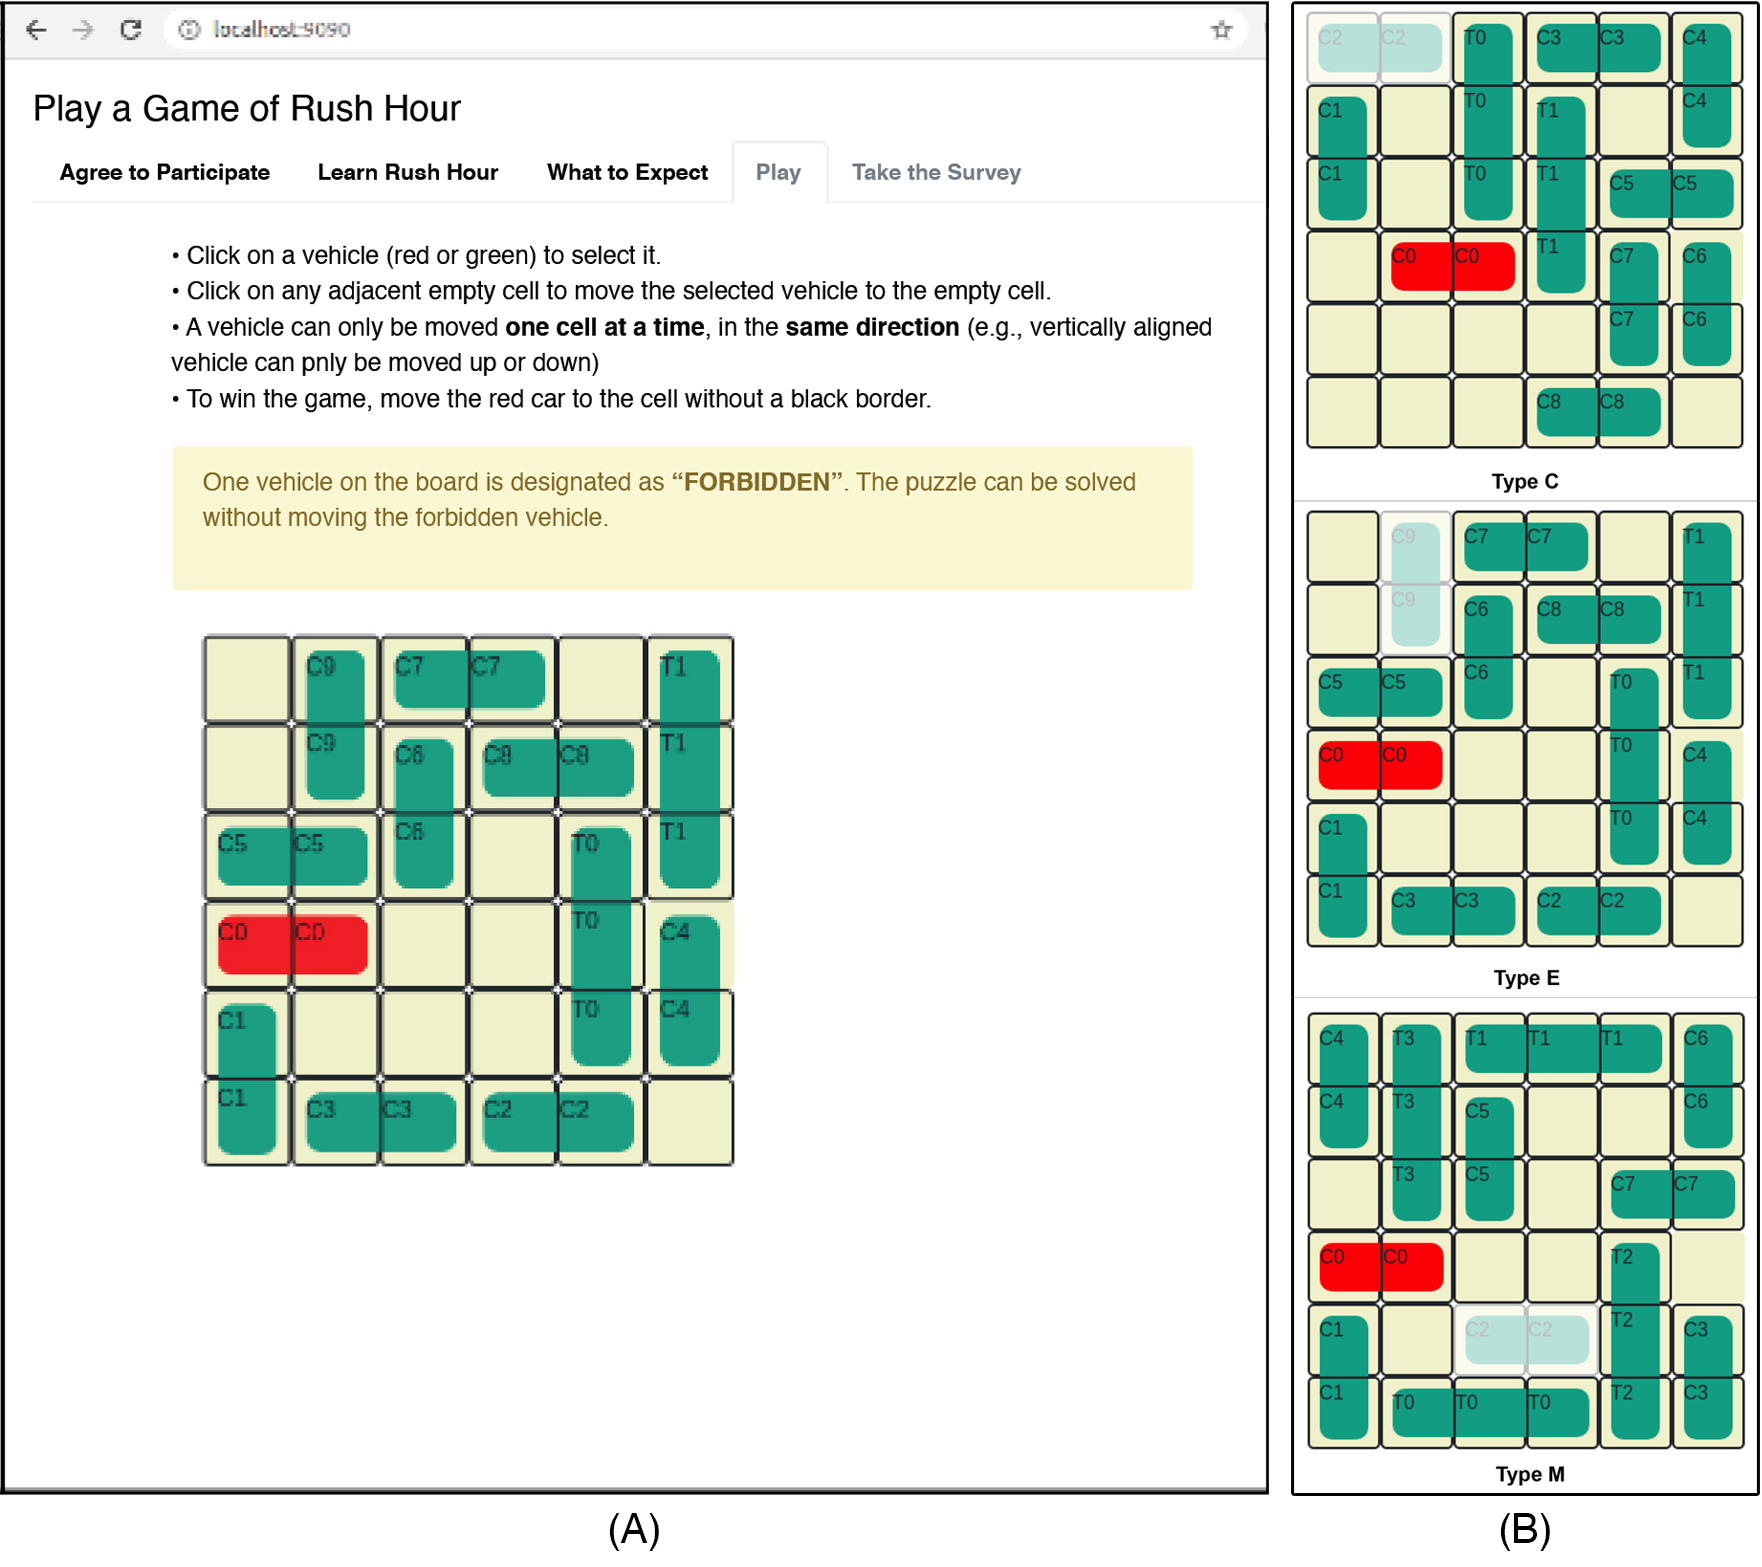
\includegraphics[width=0.8\columnwidth]{img/figure6.jpg}
  \caption{(A) Rush Hour planning task Web interface. The forbidden vehicle for this configuration is $C_9$. (B) Rush Hour puzzle configuration types with forbidden vehicles highlighted.}
  \label{fig:ui}
\end{figure}

We use ten Rush Hour planning tasks for the experiment. 
For analysis purposes (see Appendix), we separate the ten puzzles into three groups by the position of the forbidden vehicle. 
As shown in Figure~\ref{fig:ui}(B), type \textbf{C} has the forbidden vehicle in the \textbf{c}orner of the board. 
Type \textbf{E} has the forbidden vehicle on an \textbf{e}dge. 
Type \textbf{M} has the forbidden vehicle in the \textbf{m}iddle. The experiment uses four puzzles of type C, five puzzles of type E and one puzzle of type M.


\subsection{The Learning Methods}
\label{sec:learningmethods}
Our solution to the Human-aware Intervention Problem uses machine learning to predict whether \undesired will be reached in $k$ moves, given \historyDef, where $k=\lbrace 1,2,3\rbrace$.
To produce the learned models, we first partition the 136 human user solution from the experiment into training (70\%) and test (30\%) sets. 
To produce the \historyDef for a user, the user's solution is pre-processed to only include the moves until one step, two steps and three steps before the forbidden vehicle was moved for the first time. 
For example, in a  solution $O=\lbrace o_1, \ldots, o_i\rbrace$, if a user moved the forbidden vehicle in step $i$, we generate three observation traces $O_1=\lbrace o_1, \ldots, o_{i-1}\rbrace$, $O_2=\lbrace o_1, \ldots, o_{i-2}\rbrace$ and $O_3=\lbrace o_1, \ldots, o_{i-3}\rbrace$ corresponding to that user. 
Observation traces of type $O_1$ were used to train the model for $k=1$, observation traces of type $O_2$ were used to train the model for $k=2$ and so on.
Given the sequence of actions in the user's solution, the corresponding state after each move required for \historyDef is derived using the STRIPS planning model for the corresponding Rush Hour puzzle.
We use the features based on state and features based on actions together to train five classifiers with 10-fold cross validation for each value of $k$. 
We explore a number of classifiers: the decision tree, random forest, K-nearest neighbor, Logistic Regression and Naive Bayes. 
The classifiers are used in the supervised learning mode. 
We summarize the parameters used in each learning method below:
\begin{itemize}
\item \textit{Decision Tree:} We use the J48 classifier available on the WEKA platform \cite{hall09}. This classifier implements the C4.5 algorithm \cite{quinlan1993c45}. The decision tree classifier is tuned to user pruning confidence$=$0.25 and the minimum number of instances per leaf$=$2.
\item \textit{Random Forest:} This classifier is tuned to use bagging with 100 iterations and a base learner. These configuration parameters are available on the WEKA platform. 
\item \textit{k Nearest Neighbor (KNN):} We use this classifier with a Euclidean distance metric, considering the value $k=1$
\item \textit{Logistic Regression:} This classifier is tuned for ridge parameter $= 1.0E-8$.
\item \textit{Naive Bayes:} This classifier is tuned with the supervised discretization$=$\texttt{True}.
\end{itemize}


\subsubsection{Human-aware Intervention Accuracy}
We used the learned models on the test data set to predict whether the user should be intervened given \historyDef. 
In order to evaluate the classifier accuracy, we first define true-positives, true-negatives, false-positives, false-negatives for the human-aware Intervention Problem. 
A true-positive is when the classifier correctly predicts that \undesired will be reached in $k$ moves given \historyDef.
A true-negative is an instance where the classifier correctly predicts that the \undesired will not be reached in $k$ moves.
A false-positive is an instance where the classifier incorrectly identifies that the \undesired will be reached in $k$ moves.
A false-negative is an instance where the classifier identifies that the \undesired will not be reached in $k$ moves, but in fact it does.


Table~\ref{tab:rupsraccuracy} summarizes the precision, recall and F-score for predicting intervention for $k=\lbrace 1,2,3 \rbrace$. 
It can be seen that the Logistic Regression classifier performs the best with high precision/recall compared to other classifiers when predicting intervention for $\lbrace k=1,2\rbrace$
When $k=3$, the Logistic Regression classifier predicts intervention with high recall but slightly lower precision. 
The precision of the decision tree classifier improves for higher values of $k$.
However, the recall and F-score drop when $k=3$.
The Naive Bayes classifier reported the lowest precision compared to all other classifiers for any value of $k$.

\begin{table}[pbt]
\resizebox{\textwidth}{!}{%
\begin{tabular}{|l|l|l|l|l|l|l|l|l|l|}
\hline
\multicolumn{1}{|c|}{\multirow{2}{*}{Classifier}} & \multicolumn{3}{c|}{$k=1$} & \multicolumn{3}{c|}{$k=2$} & \multicolumn{3}{c|}{$k=3$} \\ \cline{2-10} 
\multicolumn{1}{|c|}{} & \multicolumn{1}{c|}{Precision} & Recall & F-score & Precision & Recall & F-score & Precision & Recall & F-score \\ \hline
Decision Tree & 0.70 & 0.90 & 0.89 & 0.80 & 0.95 & 0.87 & 0.89 & 0.81 & 0.85 \\ \cline{1-1}
Random Forest & 0.76 & 0.9 & 0.83 & 0.75 & 0.86 & 0.80 & 0.86 & 0.90 & 0.88 \\ \cline{1-1}
KNN & 0.89 & 0.76 & 0.82 & 0.86 & 0.86 & 0.86 & \textbf{0.95} & \textbf{0.90} & \textbf{0.93} \\ \cline{1-1}
Logistic Regression & \textbf{0.91} & \textbf{0.95} & \textbf{0.93} & \textbf{0.87} & \textbf{1} & \textbf{0.93} & \textbf{0.91} & \textbf{0.95} & \textbf{0.93} \\ \cline{1-1}
Naive Bayes & 0.73 & 0.90 & 0.81 & 0.74 & 0.86 & 0.83 & 0.68 & 0.90 & 0.78 \\ \hline
\end{tabular}
}%
\caption{Precision, Recall and F-scores for the prediction accuracy of the Human-aware Intervention learned models. Best values are in bold.}
\label{tab:rupsraccuracy}
\end{table}



\subsubsection{Human-aware Intervention as a Plan Recognition Problem}
Recall that in Section~\ref{sec:distinguishing}, we showed that it is possible to frame the Intervention Problem as a Plan Recognition task, where the observer models the \undesired and \desired as the set of likely goals of the user.
Then, we can implement the observer in the Rush Hour puzzle solving task as a probabilistic Plan Recognition agent that solves the Plan Recognition Problem $T=\langle \domainUser, \mathcal{G}, \historyDef, Prob \rangle$, where \domainUser is the planning domain, the set of likely goals $\mathcal{G}=\lbrace \mathrm{u},\mathrm{d}\rbrace$, \historyDef is the observation sequence and $Prob$ is a probability distribution over $\mathcal{G}$. 
By compiling the observations away into the domain theory, Ramirez and Geffner showed that, it is possible to use an automated planner to find plans that are compatible with the observations and use these observation compatible plans to determine what the most likely goal and plan \cite{ramirez2010probabilistic} is for the user. 
They evaluated the approach on benchmark planning domains.

If the observer can recognize \undesired as the most likely goal given the observations, then the user can be intervened at that point.
We adapt the Plan Recognition as Planning (PRP) algorithm proposed by \cite{ramirez2010probabilistic}, to evaluate how the observer
executing PRP recognizes the most likely goal given the observation traces $O_1=\lbrace o_1, \ldots, o_{i-1}\rbrace$, $O_2=\lbrace o_1, \ldots, o_{i-2}\rbrace$ and $O_3=\lbrace o_1, \ldots, o_{i-3}\rbrace$, corresponding to $k=\lbrace 1,2,3\rbrace$.
We use the same test set from the classifier evaluation to evaluate the PRP algorithm in predicting intervention.
This experiment also allows us to evaluate the PRP algorithm on plans generated by human users.

In order to evaluate the PRP accuracy, we first define true-positives, true-negatives, false-positives, false-negatives for the observer implementing the PRP algorithm. 
A true-positive is when the observer correctly selects \undesired as the most likely goal given the observation traces $O_1$, $O_2$ and $O_3$ for $\lbrace k=1,2,3\rbrace$ respectively.
A true-negative is an instance where the observer correctly does not select \undesired as the most likely goal given the observation traces. 
A false-positive is an instance where the observer incorrectly identifies \undesired as the most likely goal given the observations. 
A false-negative is an instance where the observer incorrectly does not select \undesired as the most likely goal but in fact it is.

Table~\ref{tab:prp} summarizes the precision, recall and F-score for deciding to intervene correctly for $k=\lbrace 1,2,3\rbrace$ using PRP. 
PRP requires goal priors as an input to the algorithm. 
We used the Fast-Downward planner \cite{richterWestphal10.jair.LAMA} to generate satisficing plans that are compatible with the observations for PRP. 
Our assumption of the users' plans being satisficing is justified by the findings reported in Section~\ref{ap:distribution} in the Appendix. 
It shows that the majority of the users did not find optimal length solutions.
In order to analyze the algorithm performance on different goal priors, we set three levels: (1) uniform goal priors, where \undesired and \desired are equally likely (i.e., $P(\mathrm{u})=P(\mathrm{d})$), (2) \undesired is more likely and (3) \desired is more likely. 
We decided on these prior probability distributions based on the forbidden vehicle's position on initial game configurations used in the experiment. 
We set a higher value for \undesired to indicate the situation where the forbidden vehicle is not blocked by other vehicles. 
As a result, the user will likely move it. 
We set \desired as high if the forbidden vehicle is blocked in the initial configuration, to indicate that the user will be less likely to move it. 
The uniform probability is the default.

It can be seen that PRP accuracy in predicting when the \undesired will be reached is lower compared to the learned models for all levels of $k$.
The accuracy does not change with values of $k$. 
This observation is consistent with the accuracy of the logistic regression model (i.e., the best performing learned model).
When the goal priors are biased in favor of the undesirable state, the prediction accuracy slightly improves. 
However, giving a higher prior to \undesired contradicts with our intervention models' assumptions that the user wants to avoid the undesirable state, which implies that $P(\mathrm{u})$ must be low.




\begin{table}[tpb]
\resizebox{\textwidth}{!}{%
\begin{tabular}{|l|l|l|l|l|l|l|l|l|l|}
\hline
\multirow{2}{*}{Goal Priors} & \multicolumn{3}{c|}{$k=1$} & \multicolumn{3}{c|}{$k=2$} & \multicolumn{3}{c|}{$k=3$} \\ \cline{2-10} 
 & Precision & Recall & F-score & Precision & Recall & F-score & Precision & Recall & F-score \\ \hline
Uniform & 0.67 & 0.56 & 0.61 & 0.67 & 0.56 & 0.61 & 0.56 & 0.67 & 0.61 \\ \cline{1-1}
$P$(\undesired) = 2$\times P$(\desired) & 0.69 & 0.61 & 0.65 & 0.69 & 0.61 & 0.65 & 0.69 & 0.61 & 0.65 \\ \cline{1-1}
$P$(\desired) = 2$\times P$(\undesired) & 0.67 & 0.56 & 0.61 & 0.67 & 0.56 & 0.61 & 0.67 & 0.56 & 0.67 \\ \hline
\end{tabular}
}%
\caption{Precision, Recall and F-scores for solving the r-UPSR problem as a Plan Recognition problem with the Probabilistic Plan Recognition as Planning algorithm.}
\label{tab:prp}
\end{table}


%===========================================================================================================
%%===========================================================================================================
\section{Discussion}
\label{sec:discussion}
In this chapter, we formalized a family of Intervention Problems and showed that how these problems can be solved using a combination of Plan Recognition methods and classification techniques to decide when to intervene.
The Unsafe Suffix Intervention Problem uses automated planners to \textbf{project the remaining suffixes} and extract features that can differentiate unsafe remaining suffixes from the safe remaining suffixes. 
In contrast, the Human-aware Intervention Problem uses \textbf{only the observed history \historyDef} to extract features that can separate the solutions leading to undesirable state from the solutions that will avoid it.
We compared the Unsafe Suffix Intervention and Human-aware Intervention using the state-of-art Plan Recognition approaches in the literature as the baseline and found that our learning based intervention solutions dominate the existing Plan Recognition algorithms for both benchmark Intervention Problems and a new intervention benchmark, Rush Hour.

In Unsafe Suffix Intervention, when intervention models are trained using features extracted from the Intervention Graph, all the learned models chose distance to \undesired and Risk as the dominant features. We were not able to identify clear dominant features in learned models built with plan space sampling. 
In Human-aware Intervention, the best performing learned model for $k=\lbrace 1,2,3\rbrace$, the logistic regression classifier, selected  \texttt{backtracks}, \texttt{blocks}, \texttt{frees}, \texttt{reset}, \texttt{freebci}, \texttt{freebcd}, \texttt{freegci}, \texttt{freegcd}, \texttt{mgc}, \texttt{mbc} and \texttt{moved} as the features for determining intervention.

We show that both the Unsafe Suffix Intervention Problem and the Human-aware Intervention Problem can be re-framed as Plan Recognition problems and use the recognition process to decide intervention. 
The results prove the feasibility of this approach. 
However, compared to the proposed machine learning based solutions, Plan Recognition based intervention accuracy is low for both benchmark Intervention Problems and the Rush Hour Intervention Problem. 
The requirement of setting goal priors for Plan Recognition is an issue that must to be overcome for intervention. 
This is because during execution, the user's plan may be subverted to achieve the undesirable state by environmental factors (such as attackers and hidden knowledge) regardless the priors. 
In Unsafe Suffix Intervention, we find that even when we assume reasonable goal priors, if the plans for \undesired share long common action sequences with plans for \desired, Plan Recognition as Planning (PRP) approaches fail to correctly disambiguate between  \undesired and \desired. 
This affects the overall intervention accuracy by producing many false alarms and misses. 
In the intervention scenario we simulated with the Rush Hour domain, setting goal priors is even more problematic. 
This is because the user is informed about the presence of a forbidden vehicle and that the puzzle can be solved without moving it prior to executing the planning task. 
The result of that information being given to the user is that the goal prior for \undesired is low compared to \desired. 
In our experiments, we show that the recognition accuracy for PRP approach drops when goal priors are set this way. 
We remove the dependency on goal priors by using features of projected remaining suffixes (in Unsafe Suffix Recognition) and the observed partial solution \historyDef (in Human-aware Intervention) to learn the differences between safe and unsafe plans from example training data and using the learned models to predict intervention.

Our findings comparing PRP and the learned model for Human-aware Intervention show that deciding to intervene based on plan cost differences (PRP) is not sufficient, especially when intervening human users.
As seen in from the solution length distributions in Section~\ref{ap:lengroups}, the longer the human user spends exploring the state space, the higher the likelihood that his partial plan will get closer to \undesired. 
Therefore, we argue that intervention for human users require representations that capture characteristics of the actor's behavior in addition to the planning representations. 
The features based on actions and the features based on state extracted from \historyDef we propose for learning Human-aware Intervention capture the behavior patterns of the human user and as a result produce accurate learned models. 
However, a limitation of our proposed approach is that some features in the feature vector are domain-specific. 
Therefore, adopting the proposed approach in different planning domains may require feature engineering.


There are other methods one could use for generating \Suffixes, which we will explore in future work.
In Unsafe Suffix Intervention, we generated \Suffixes from the \historyEndState using an automated planner without considering the observations in \historyDef.
We then compared the suffixes in \Suffixes to an observation compatible reference plan.
\cite{ramirez2009plan, ramirez2010probabilistic, sohrabi2016plan} propose methods to compile the observations into the domain theory, which allows the planner to find observation compatible plans.
We can use this technique to also find observation compatible suffixes in \Suffixes.
By making the both \Suffixes and the reference plan compatible with the observations, we believe the plan distance features will be more accurate for the Plan Space Sampling method.



%===========================================================================================================
%%===========================================================================================================
\section{Closing Remarks}
\label{sec:closing}
Intervention is a necessity for online assistive agents and safety critical decision making, where an observer determines how to guide an user toward a desirable outcome while avoiding undesirable outcomes. 
We propose Intervention as a solution to this problem and introduced two algorithms that combine automated planning and machine learning to decide whether or not the user's likely plan will avoid the undesirable state. 
Representing the user's task as a planning problem allows us to extract features of the user's plan space that can be used to produce learned models to recognize when intervention is required. 
Our first solution Unsafe Suffix Intervention, uses automated planning to project the remaining suffixes and extract features to differentiate between safe suffixes that avoid the undesirable outcome and unsafe suffixes that do not avoid the undesirable outcome. 
The second solution, Human-aware Intervention uses only the observed plan to extract features that can differentiate between safe and unsafe solutions. 
We showed that the two learning based intervention solutions dominate the state-of-the-art Plan Recognition algorithms in identifying when intervention is required.

In this work, our objective was to identify, given a sequence of observations, whether the user requires intervention while minimizing false positives and negatives. 
For our current implementation we assumed that the intervention comes in the form of a block or an alert message. 
The natural next step following intervention is helping the user decide what to do next. 
This extension is particularly important for observers where the user is a human user who would like to be guided towards the goal instead of being given the solution outright (e.g., an automated tutoring agent). 
We identify two sub-problems in helping the user decide what to do next. 
First, we can explore how automated planning can be used to gradually probe the search space of the remaining planning task following intervention. 
In certain cases, the user may want a quick, well-focused help. 
For example, in the Rush Hour puzzle, the observer can suggest the first move in the shortest remaining plan that avoids the forbidden vehicle as a hint after intervening. 
In other cases, the user would prefer more abstract suggestion. 
For example, in the Rush Hour puzzle, the observer can suggest the vehicles that must be moved to solve the puzzle (i.e., the landmarks of the planning task). 
In various stages of the puzzle solving task, the user may opt to use these suggestions differently. 
The second sub problem is explaining intervention and the follow-up to intervention. 
We can explore how effective different explanation models (e.g., contrastive, selective) are in explaining intervention and intervention Recovery to human users.

There are several other extensions to our current intervention framework, that we would like to explore as future work. 
In the planning domains we used to model intervention tasks, we assumed that the user's actions are deterministic and there is only one undesirable state that needs to be avoided. 
It is possible to relax these two assumptions and explore intervention in non-deterministic environments where the user needs to avoid multiple undesirable goals. 
However, in order for intervention to be meaningful, the intervention planning domains need to be descriptive enough to model complex tasks. 
We can explore the feasibility of adopting scenario building game environments like Minecraft for this purpose.


\chapter{Interactive Human-aware Intervention}
\label{chap:ch6}
Using the Rush Hour domain, we study how an intervention model can be extended to recover from intervention and help users complete cognitively engaging tasks by providing helpful hints. 
In the context of the Rush Hour puzzle solving task, a hint is a piece of information about the Rush Hour planning problem. 
We design helpful hints to allow the user to carefully probe the search space of the Rush Hour STRIPS planning task described in Section~\ref{sec:rushhourstrips} in
Chapter~\ref{chap:ch5} while avoiding the undesirable state.
Existing plan and goal recognition algorithms do not define a method for the user (or the software agent) to recover when the observer recognizes an undesirable state is developing and/or imminent.
In this chapter, we address that limitation by designing four helpful hints the observer presents to the user after intervening.
\begin{itemize}
\item The minimum remaining number of moves
\item The next best move
\item The vehicles that must be moved
\item Restart puzzle
\end{itemize}


In Chapter~\ref{chap:ch5}, we presented the Human-aware Intervention problem for the Rush Hour puzzle task as a tuple
$\mathcal{I} = (D, \desired, \undesired, \historyDef, \presentedAction, \mathcal{X}_\Diamond)$ be a tuple where
  $D=\langle F, A, \initialState \rangle$ is a planning domain,
  $\desired \subset F$ is a desirable state,
  $\undesired \subset F$ is an undesirable state,
  $\historyDef = ( o_1 [s_1], o_2 [s_2], \ldots, o_{i-1} [\historyEndState])$ is a history of previously observed actions and states, which started from \initialState with the implied resulting states in brackets.
  \presentedAction is the \emph{presented action} that the user would like to perform, and
  $\mathcal{X}_\Diamond = \emptyset$ because we can not use an automated planner to extract suffixes when a human user is solving the planning task.
The \textnormal{Intervention Problem} is a function $intervene (\mathcal{I}) :  \mathcal{I} \rightarrow \{No, Yes\} $
that determines for the presented action \presentedAction whether to intervene.
For Rush Hour, the observer relies on those implied states instead of just the actions to decide intervention.
Because we model the Rush Hour planning task as a deterministic state transition system,  it is easy to map between actions and states.

For the study discussed in this chapter, the observer uses the Rush Hour Human-aware Intervention model configured to use the lowest level of sensitivity (i.e., $k=1$).
When $k=1$, the observer predicts intervention one move before undesirable state occurs.
For each action the user executes, the observer solves the Human-aware Intervention problem $\mathcal{I}$ if the $intervene (\mathcal{I}) :  \mathcal{I} \rightarrow \{Yes\} $, the observer displays the hints to help the user decide what to do next.
We evaluate the effectiveness of the proposed intervention recovery approach with a human subject experiment.


\section{Motivation}
When a human user is learning to use a new software application, it can be helpful to have a passive observer that can intervene to help the user reach his intended goal. 
This is particularly important when using the software imposes a significant cognitive load on the user and as a result the user's plan to accomplish the intended goal can become vulnerable to unintended actions or events.
For this study, we simulate the human user learning to use a new software application with the Rush Hour puzzle solving task, 
In addition to the cognitive load, there may be information in the domain (e.g., Rush Hour puzzle, new software application) hidden to the user that may increase the likelihood that the user's intended goal will have unintended consequences. 
For example, at the start of the Rush Hour puzzle solving task, the user does not know what the forbidden vehicle is.
Since the Rush Hour puzzles can be solved without moving the forbidden vehicle, moves that enable the forbidden vehicle to be moved later are \textit{unhelpful moves} and signal to the observer that the human user needs help. 
Intuitively, any action that moves the forbidden vehicle triggers the undesirable state.
The observer's decision making problem is to recognize when the user is making unhelpful moves before the undesirable state is triggered with varying sensitivity levels.

The rest of this chapter is organized as follows. We first revisit the dimensions of the Intervention Problem the observer solves during the Rush Hour puzzle solving task. 
As summarized in Table~\ref{tab:dim4}, this is a single-user Intervention problem, where no attackers, or competitors are present. 
Second we discuss related work on improving interactivity in human-agent collaborative environments, specifically focusing on Explainable Artificial Intelligence.
Third, we formally define the four helpful hints.
Fourth, we describe the experimental protocol and the software tools developed to support the experimental setup.
Finally, we present the findings of our study to answer the following questions.
\begin{itemize}
\item What are the most frequently used hints in different stages of the Rush Hour planning task?
\item Does seeing hints have an effect on the solution length?
\item Does the hints help move the user closer to the optimal solution?
\item Does seeing hints have an effect on the number of times the forbidden vehicle was moved?
\end{itemize}

\begin{table}[ptb]
\begin{tabular}{|l|l|}
\hline
\textbf{Dimension} & \textbf{Domain Specific Properties} \\ \hline
Actors in the environment & User, Observer \\ \hline
Goals hidden to the observer & \begin{tabular}[c]{@{}l@{}}User's goal not hidden\\ One or more known undesirable states\end{tabular} \\ \hline
Types of observations & The user's actions and states resulting from actions \\ \hline
Noise in observations & None \\ \hline
Intervention recovery & Offer helpful hint \\ \hline
\end{tabular}
\caption{Dimensions of the Human-aware Intervention Problem}
\label{tab:dim4}
\end{table}


\section{Related Work}
Developing human-aware intervention models must be predicated upon understanding how human users solve a planning task. 
The human subject study described in Chapter~\ref{chap:ch5} addressed this requirement, where we used the plans generated by human users for Rush Hour planning tasks to generate learned models that can recognize when the user is making unhelpful moves and needs help.
When the observer generates an intervention for the Rush Hour planning task (as an alert message displayed on the screen), it signals that an undesirable state is developing, which the user can not recognize on his own at the time.
Although the intervention alert message may convey to the user that their action might cause undesirable consequences, given the cognitive load imposed by the task he/she may need help in framing the decision about what action to execute next. 
Studies have shown that users want some positive outcome from their action and are willing to accept that negative outcomes are a possibility \cite{good2005stopping, govani2005, debatin2009facebook, byrne2016}. 
Therefore, a solution cannot simply block the user from taking the action, but instead needs to assist them deciding what to do and recover from the unhelpful state. 
In this chapter, our objective is to study the impact of giving information about the Rush Hour planning problem on intervention recovery.

\subsection{Improving Interactivity with Explanations}
When a human user and an agent collaborate in an environment, having their own knowledge of the world, knowledge about goals and plans to achieve them, the agent may take actions that the human user does not expect. 
For example, in the Rush Hour domain, when the observer intervenes the human user, it comes as  surprise because the user can not recognize the developing undesirable state.
Recent research in Explainable Artificial Intelligence (XAI) addresses different challenges related to making AI systems transparent and interactive in human-agent collaborations. Specifically in the area of explaining the behavior of \textit{rebellious agents} \cite{coman2015case}, where an agent with goal reasoning capabilities may rebel by rejecting or revising the goals and plans a human teammate may expect it to follow, the explanation helps to build trust and understanding between the human and the agent. 
Rebellion has many positive motivations; for example in situations where the current plan execution will pose a threat to safety of the agent or the human, goals becoming unachievable due to resource constrains and ethical conflicts, differences in information access between the agent and the human.
Similar to an agent who intervenes, a rebellious agent increases unpredictability when other agents or human users interact in the environment.
In this situation, it is beneficial for the rebellious agent to have the ability to explain its behavior.
In 2016, legal measures were adopted in the European Union that grant the individuals affected by automated decision making with a ``right to explanation'' \cite{eu2016}.

Most efforts on improving interpretability of AI systems have focused on providing transparency to decision making using machine learning \cite{ribeiro2016, lundberg2017, slack2020}. 
Research on improving interpretability and interactivity of AI systems that use automated planning for decision making has become popular in the recent years. Sohrabi et al. \citeyear{sohrabi2011} describe a technique to help humans understand a plan produced by an automated planner. Chakraborti et al. \citeyear{chakraborti2019} describe a method to generate explanations by reconciling the domain models of the agents and describing the differences between the models. 
Several other work focus on explaining why a planner chose a particular action rather than a different one
\cite{langley2017explainable, fox2017xai}.

Prior efforts in explaining rebel behavior in agents consider explaining actions with harmful effects when the rebellious agent rejects to execute them \cite{briggs2015,greggsmith2015}.
Dannenhauer et al. \citeyear{dannenhauer2018explaining} proposes a method for a rebellious agent with goal reasoning capabilities to explain it's planning and goal reasoning decisions. 
When a goal reasoning rebellious agent rejects a goal, it needs to show that it can not find a plan to achieve that goal without violating the conditions (e.g., safety, ethical etc.).
The authors propose a question/answer dialog model where (1) the rebellious agent questions the current plans that violate the conditions and tries to find alternative plans or (2) the human questions the rebellious agent about the initial plan to find possible (safe) ways to achieve the goal.
The question/answering dialog model uses the explainable planning framework proposed by Fox et al. \cite{fox2017xai}.
In that framework, the authors argue that questions in explainable planning must be designed to help the questioner \textit{uncover a piece of knowledge that the questioner does not have but believes to be available in the system} while avoid the obvious statements.  
For an example, suppose we our observer has the capability to explain intervention. When the user asks ``why did you intervene?'', the answer should not be ``\textit{because it will trigger the undesirable state}'' because that is obvious.
They present six questions: (1) ``Why did you do action A'', (2) ``And why didn’t you do something else(that I would have done)?'', (3) Why   is   what   you   propose   to   do   more   efficient/safe/cheap than something else (that I would have done)?, (4) ``Why can’t you do that?'', (5)``Why do I need to replan at this point?'', (6) Why do I not need to replan at this point?''
They also discuss what constitutes a response to these six questions from an automated planning perspective.


\section{Hints: A Different Model of Explanation}
The interactivity we bring in to Human-aware Intervention with helpful hints is different from the existing work on using explanations to improve how humans understand decision making of planning systems.
In human-aware intervention, the human user acts as the planner but the complexity of the problem challenges the human user's ability to find a solution that avoids the undesirable state.
The observer's role is to guide the user upon recognizing that the user is executing a plan that may result in the undesirable state.
Following the definition of an explanation advanced by Fox et al. \citeyear{fox2017xai}, we designed the hints to help the user uncover pieces of information about the Rush Hour planning problem so that using the hints will help the user move toward the goal safely.
Instead of engaging the human user in a question and answer dialog model, every time the observer intervenes, the hints are presented as options for the human user to choose.
We consider the Rush Hour STRIPS planning task to generate the hints.

\subsection{Cost Optimal Solutions in the (Modified) Rush Hour Planning Task}
\label{sec:costoptimal}
Let us revisit the Rush Hour instance introduced in Chapter~\ref{chap:ch5}. As illustrated in Figure~\ref{fig:board}, several cars (size=2) and trucks (size=3) are arranged on the board, which has only one exit.
The objective of the game is to move the vehicles on the board in such a way that the target car (shown in red) can be moved out of the exit on the right edge of the board. Solution to the Rush Hour puzzle is a sequence of legal moves (a \textit{plan}) that transforms the initial board state shown in Figure~\ref{fig:board}(A) to the goal state in Figure~\ref{fig:board}(B). 
Actions in the plan may have a cost that assigns a non-negative value to the action schema defined in the STRIPS domain definition. 
The cost function is given as $C: Op \rightarrow \mathbb{R}^0_+$. 
The cost of the plan $c(\pi)$ is  $\sum(c(a_i))$. The optimal solution, the optimal plan $\pi^*$, minimizes the cost. 

\begin{figure}[tpb]
  \centering
    	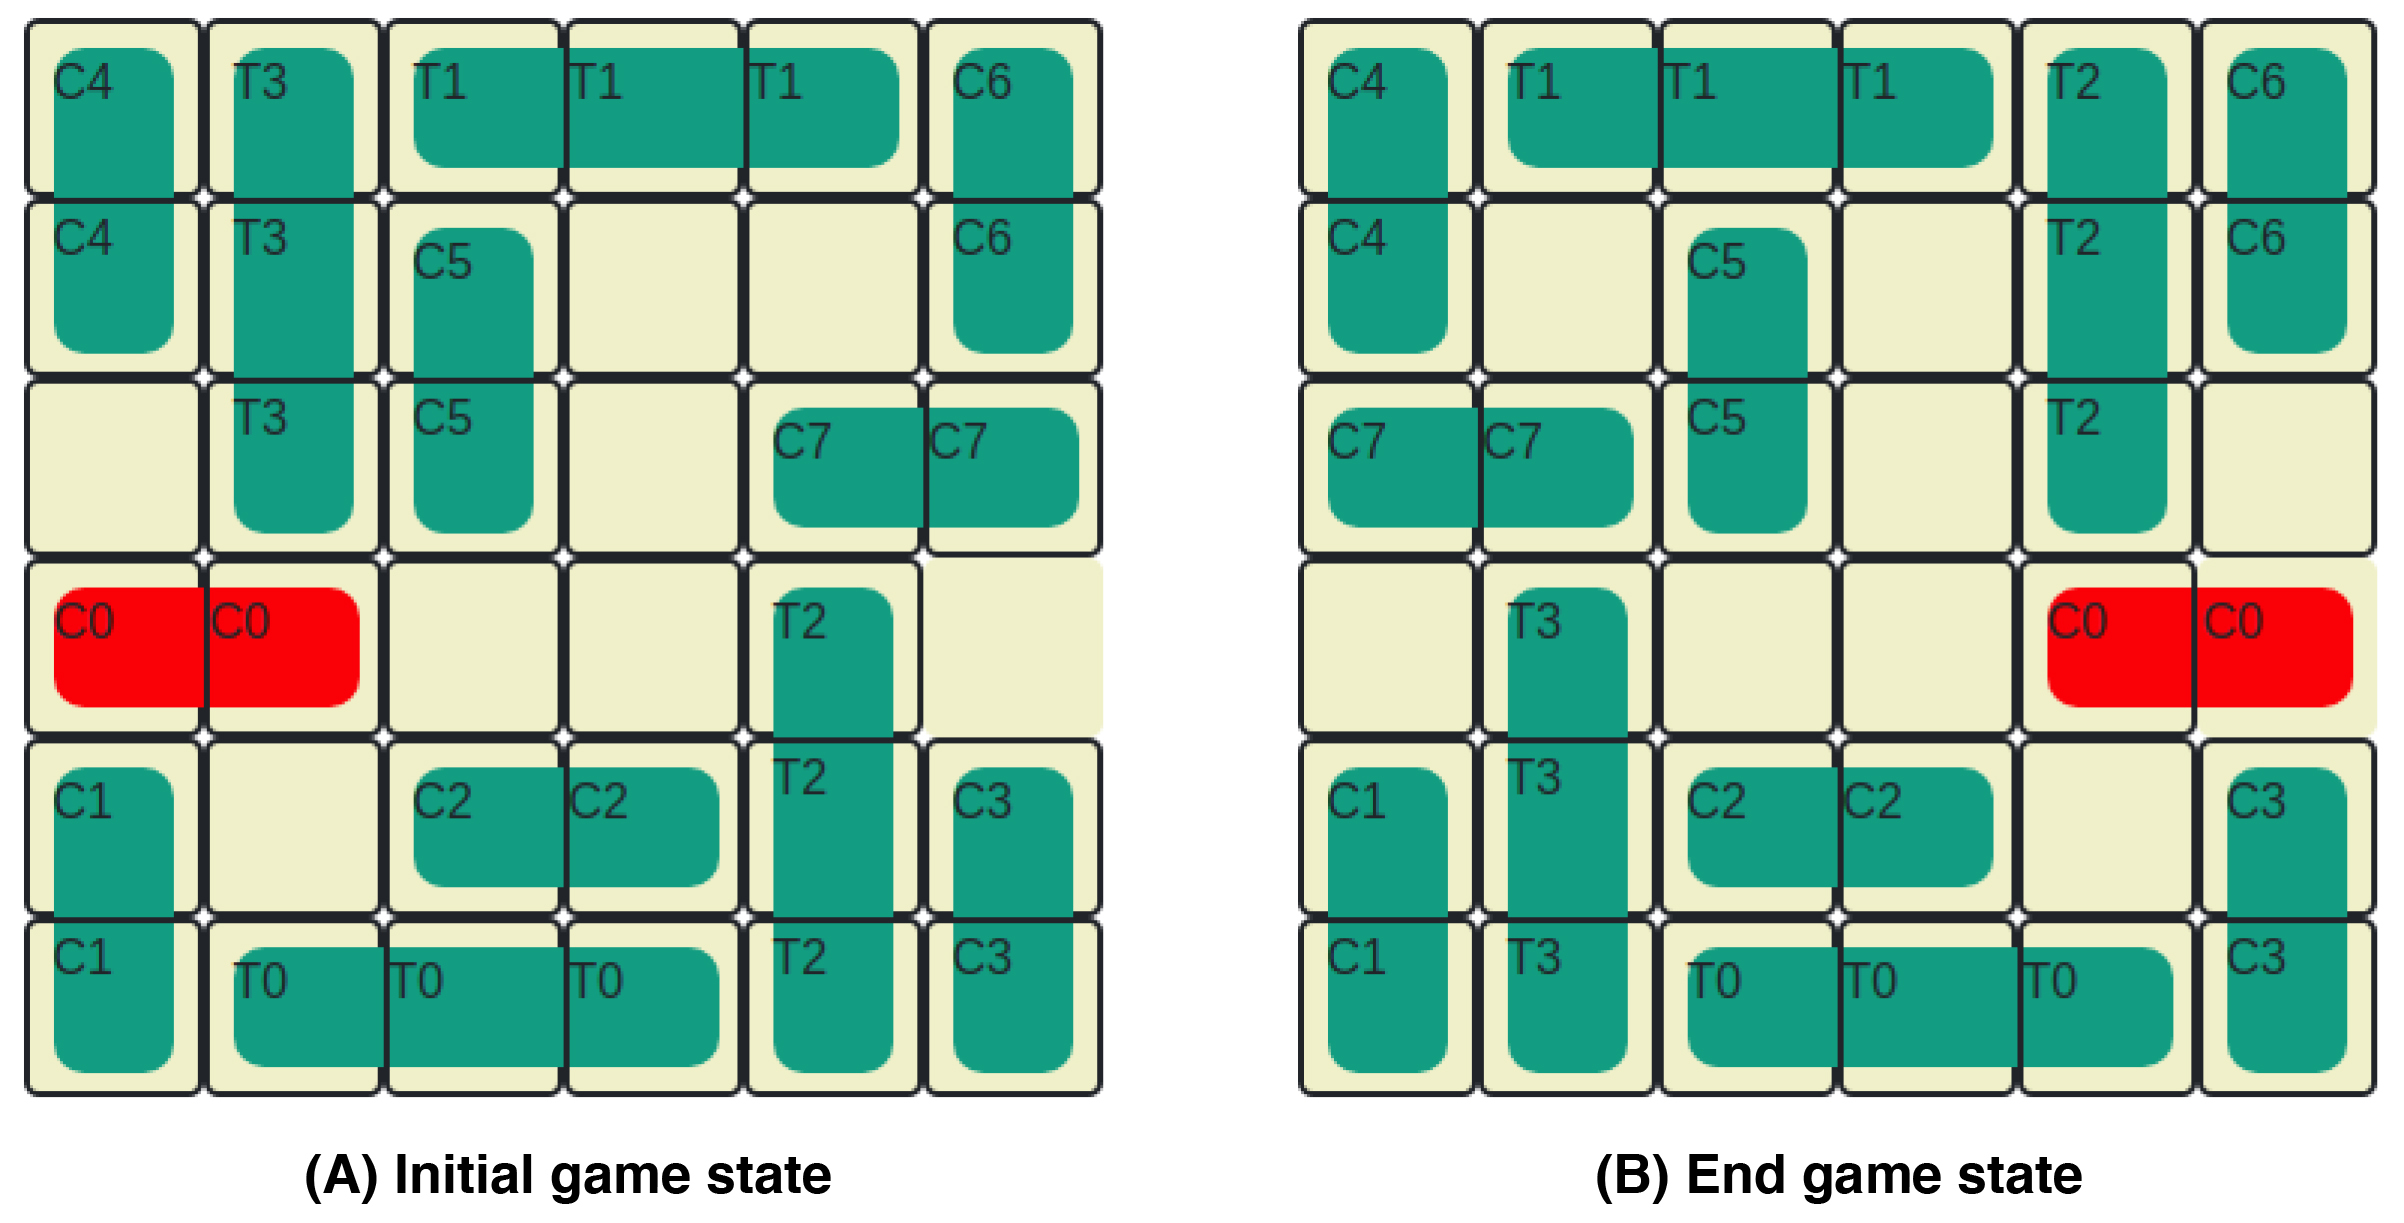
\includegraphics[width=0.7\textwidth]{img/figure4.jpg}
    	\caption{A Rush Hour instance}
    	\label{fig:board}
\end{figure}

An off-the-shelf automated planner can be used on the Rush Hour STRIPS planning task defined in Section~\ref{sec:rushhourstrips} in
Chapter~\ref{chap:ch5} to find a cost optimal plan.
A given Rush Hour instance may have multiple cost optimal solutions.
We recognize two optimizing criteria for a solution of the Rush Hour STRIPS planning task:
\begin{itemize}
\item the number of moves
\item the number of vehicles moved
\end{itemize}
In this study, we consider the number of moves as the optimizing criteria where we assume all moves are uniform cost equal to 1.
For the puzzle shown in Figure~\ref{fig:board}(A), the cost optimal solution, if the number of moves is considered as
the optimizing criteria, consists of 21 moves. 
If optimized for the number of vehicles moved,
the puzzle can be solved optimally by moving only 8 vehicles.

We modify the standard Rush Hour planning task by introducing a forbidden vehicle. 
For example, vehicle C2 in Figure~\ref{fig:board}(A) is forbidden. 
When the forbidden vehicle is moved, the undesirable state is triggered.
The human user does not know what the specific forbidden moves are, but he knows that \textit{some} moves are forbidden.
The planning task can be solved without moving the forbidden vehicle.
Therefore, if the human user moves the forbidden car while solving the Rush Hour planning task, it indicates that he is moving away from a cost optimal solution and needs help.
Because moving the forbidden vehicle is unnecessary, an automated planner can be used to find cost optimal solutions to the Rush Hour planning task.
In contrast, a human user not having the heurisitic search capabilities as a planner, may make mistakes and commit to plans that are longer and may even reach the undesirable state.
For example, Table~\ref{tab:plan} shows two solutions to the same Rush Hour planning task illustrated in Figure~\ref{fig:board}.
The cost optimal solution on the left is produced by an automated planner. 
The (partial) solution on the right is produced by a human user. 
The highlighted step in the human user's solution (18$^{th}$ move) show that the user is moving the forbidden vehicle C2. 
In fact, the human user moved the forbidden vehicle twice before reaching the goal state.
The human user's solution consisted of 43 moves.
Furthermore, results from a human subject study discussed in Appendix~\ref{ap:distribution} show that human users typically find longer plans to Rush Hour planning task compared to the cost optimal solutions found by an automated planner.
Thus we conclude that the cost optimal solution to the modified Rush Hour planning task provides a reference solution against which we can compare the user’s solution.

\begin{table}[ptb]
\begin{tabular}{|c|c|}
\hline
A safe, optimal solution (21 moves) & Unsafe solution (43 moves)\\
\hline
\begin{tabular}[c]{@{}l@{}}\texttt{\textsc{move-car c0 l17 l16 l18 we}}\\ \texttt{\textsc{move-car c0 l16 l15 l17 we}}\\ \texttt{\textsc{move-truck t3 l23 l17 l29 l35 ns}}\\ \texttt{\textsc{move-car c7 l20 l21 l19 ew}}\\ \texttt{\textsc{move-car c6 l25 l19 l31 ns}}\\ \texttt{\textsc{move-truck t1 l32 l31 l33 l34 we}}\\ \texttt{\textsc{move-car c5 l28 l34 l22 sn}}\\ \texttt{\textsc{move-truck t3 l17 l11 l23 l29 ns}}\\ \texttt{\textsc{move-car c7 l21 l22 l20 ew}}\\ \texttt{\textsc{move-truck t2 l14 l20 l8 l2 sn}}\\ \texttt{\textsc{move-truck t2 l20 l26 l14 l8 sn}}\\ \texttt{\textsc{move-truck t0 l3 l2 l4 l5 we}}\\ \texttt{\textsc{move-truck t3 l11 l5 l17 l23 ns}}\\ \texttt{\textsc{move-car c7 l22 l23 l21 ew}} \\ \texttt{\textsc{move-car c7 l23 l24 l22 ew}}\\ \texttt{\textsc{move-car c5 l28 l22 l34 ns}}\\ \texttt{\textsc{move-truck t1 l33 l34 l32 l31 ew}}\\ \texttt{\textsc{move-truck t1 l34 l35 l33 l32 ew}}\\ \texttt{\textsc{move-truck t2 l26 l32 l20 l14 sn}}\\ \texttt{\textsc{move-car c0 l15 l14 l16 we}}\\ \texttt{\textsc{move-car c0 l14 l13 l15 we}}\end{tabular} &
  \begin{tabular}[c]{@{}l@{}}\texttt{\textsc{move-car c0 l17 l16 l18 we}}\\ \texttt{\textsc{move-car c0 l16 l15 l17 we}}\\ \texttt{\textsc{move-car c4 l30 l24 l36 ns}}\\ \texttt{\textsc{move-car c4 l24 l18 l30 ns}}\\ \texttt{\textsc{move-truck t3 l23 l17 l29 l35 ns}}\\ \texttt{\textsc{move-truck t3 l17 l11 l23 l29 ns}}\\ \texttt{\textsc{move-truck t1 l34 l35 l33 l32 ew}}\\ \texttt{\textsc{move-truck t1 l35 l36 l34 l33 ew}}\\ \texttt{\textsc{move-car c7 l20 l21 l19 ew}}\\ \texttt{\textsc{move-car c6 l25 l19 l31 ns}}\\ \texttt{\textsc{move-truck t1 l34 l33 l35 l36 we}}\\ \texttt{\textsc{move-truck t1 l33 l32 l34 l35 we}}\\ \texttt{\textsc{move-truck t1 l32 l31 l33 l34 we}}\\ \texttt{\textsc{move-car c5 l28 l34 l22 sn}}\\ \texttt{\textsc{move-car c7 l21 l22 l20 ew}}\\ \texttt{\textsc{move-truck t2 l14 l20 l8 l2 sn}}\\ \texttt{\textsc{move-truck t2 l20 l26 l14 l8 sn}}\\ \colorbox{LightSalmon}{\texttt{\textsc{move-car c2 l9 l8 l10 we}}}\\ \texttt{\textsc{move-truck t0 l3 l2 l4 l5 we}}\\ \texttt{\textsc{move-truck t3 l11 l5 l17 l23 ns}}\\ \texttt{\textsc{move-truck t3 l17 l23 l11 l5 sn}}\\ \texttt{\textsc{move-truck t3 l23 l29 l17 l11 sn}}\\ $\ldots$\end{tabular} \\ \hline
\end{tabular}
\caption{Solutions for the Rush Hour planning task in Figure~\ref{fig:board}(A) produced by an automated planner (left) and a human user (right). The forbidden vehicle is C2}
\label{tab:plan}
\end{table}


\subsection{Hints: Formal Definitions}
The observer solves the Human-aware Intervention problem ($\mathcal{I}$) for the Rush Hour planning task to recognize when the human user needs help and presents the hints.
In Chapter~\ref{chap:ch5}, Section~\ref{sec:learningmethods}, we presented several learned models that solve $\mathcal{I}$ to automatically recognize when the user needs help.
Hints are a special type of answer because they do not directly provide the complete solution to the question the user may ask the observer: ``\textit{why was I intervened?}'' nor do they engage the user in a dialogue. 
Our design of helpful hints allows the user to carefully probe the search space of the Rush Hour planning task while avoiding the undesirable state. 
Hints are specially useful in situations where the human user wishes to retain some autonomy over the system he is interacting with (e.g., intelligent tutoring systems).

\sloppy
Formally, a hint is a function of the search space of the Rush Hour planning problem. 
We represent the observer's Rush Hour planning problem as a tuple $P_{observer}=(D_{observer}, \dandu)$ where $D_{observer}=(F_{observer}, A_{observer}, s_0)$ is the planning domain, $\desired \subset F_{observer}$ is the desirable state, $\undesired \subset F_{observer}$ is the undesirable state.
The observer also knows the history $\historyDef=(o_1[s_1], o_2[s_2], \ldots, o_{i}[s_H])$, which consists of the moves the human user made and the state resulting from each move.
$o_i$ is the last action before intervention and $[s_H]$ is the state resulting from that action.
Note that we model the Rush Hour planning task as a deterministic problem. 
Therefore, the mapping between an action and the resulting state is straightforward.
In order to generate \historyDef, the human user solves the Rush Hour planning problem $P_{user} = (D_{user}, \desired)$ where $D_{user}=(F_{user}, A_{user}, s_0)$ is the planning domain, $\desired \subset F_{user}$ is the desirable state. 
Recall that \undesired is hidden to the user.

In order to generate the hints, the observer first modifies $P_{observer}$ as follows:
\begin{itemize}
\item $F_{observer} = F_{user} \setminus \lbrace$ \texttt{(car ?$C_i$)} or \texttt{(truck ?$T_i$)}$\rbrace$, where $C_i$ or $T_i$ is the forbidden vehicle.

$F_{observer} = F_{user} \setminus \lbrace$ \texttt{(face $?v_i$ $?d_i$)} $\rbrace$, where $v_i$ is the forbidden vehicle

$F_{observer} = F_{user} \setminus \lbrace$ \texttt{(at $?v_i$ $?l_i$)} $\rbrace$, where $v_i$ is the forbidden vehicle

\item $A_{observer} = A_{user}$
\item $s_0 = s_H$
\item $G= \lbrace \dandu \rbrace$
\end{itemize}

The $P_{observer}$ is solved by an automated planner. 
For the modified $F_{observer}$, we remove the fluents (\texttt{face}, \texttt{at}, \texttt{car}/\texttt{truck}) associated with the forbidden vehicle from the fluent set $F_{user}$.
This step instructs the planner to \textit{forget} the existence of the forbidden vehicle.
Although the forbidden vehicle is \textit{removed} from the board, we block the cells previously occupied by the forbidden vehicle in $F_{user}$ by not adding them to the fluents \texttt{free} in $F_{user}$.
This step instructs the planner not to move the other vehicles to the \textit{forgotten} forbidden vehicle's positions because those locations are not free.
These two steps force the automated planner to find solutions that do not move the forbidden vehicle and ensures that the found plans do not violate rules of the game.
The solution to $P_{observer}$ is a plan $\pi_{observer}$ from the $[s_H]$ until \desired is satisfied.
We denote the cost optimal plan as $\pi^{*}_{observer}$

\begin{definition}
\label{def:hint}
The hint is a tuple $\mathcal{N}= (F_{observer}, A_{observer}, [s_H], \desired, \undesired)$, where $F_{observer}$ is the modified Rush Hour planning domain defined above, $[s_H]$ is the state at the time intervention occurred as defined in \historyDef and \desired is the desirable goal and \undesired is the undesirable state.
The output of $\mathcal{N}$ is a property of the observer's planning problem $P_{observer}$.
\end{definition}

We study four properties of $P_{observer}$. The properties are derived considering the \textbf{cost optimal solutions} and the \textbf{fact landmarks} of $P_{observer}$.
\begin{itemize}
\item \textbf{The number of remaining moves}\\ If $P_{observer}$ is solved optimally, what is the number of moves in the cost optimal plan $\pi^{*}_{observer}$ using the number of moves as the optimizing criteria.
\item \textbf{The next best move}\\ If $P_{observer}$ is solved optimally, what is the first move to execute in the cost optimal plan $\pi^{*}_{observer}$ using the number of moves as the optimizing criteria.
\item \textbf{The vehicles that must be moved} \\
We use the fact landmark definition advanced by Hoffmann et al. \citeyear{hoffman2004lm} to find the vehicles that must be moved to solve $P_{observer}$.
Fact landmarks are the fluents that must be true for every plan that solves $P_{observer}$. 
When the fluents are grounded, the set of vehicle objects associated with the fact landmarks are the vehicles that must be moved to solve $P_{observer}$.
\item \textbf{Restart puzzle}\\
Modifies $[s_H]$ to $s_0$ so that the user solves $P_{user}$ again from the beginning.
\item \textbf{Ignore hint} \\This option is not associated with properties of $P_{observer}$.
It allows the user to disregard the hints and continue solving $P_{user}$. 
Two successive choices of \textit{Ignore hint} disables the hints and stops the human-aware Intervention process.
If the user moves the forbidden vehicle, an alert is displayed to inform the user about the forbidden action and the move is automatically undone. Figure~\ref{fig:badcar} shows the alert message.
The automatic undo blocks the user from further searching down the undesirable path and forces the user to explore a different part of the search space for $P_{user}$.
\end{itemize}

\section{Studying How Human users Solve the Rush Hour Planning Task}
We implemented an online system, which allowed human users to solve a Rush Hour planning task with and without intervention. 
As the human user solves the planning task, the system records the events that occur on the interface.
We use the system to conduct two rounds of experiments.
In the first round, human users solved the Rush Hour planning task \textbf{without the Human-aware Intervention}.
In Chapter~\ref{chap:ch5}, we used the event logs captured from this experiment as the observation history \historyDef to extract unique features that indicate when the user is getting too close to the undesirable state and needs help. 
Using the feature set, we generated learned models to predict whether or not the user's solution will reach an undesirable state before it actually happens. 
In the second round, we allow the human users to solve a Rush Hour planning task \textbf{with the Human-aware Intervention and the hints}.
In this chapter we discuss the software framework we implemented for this purpose, the experiment protocol and the findings.

\begin{figure}[tpb]
  \centering
  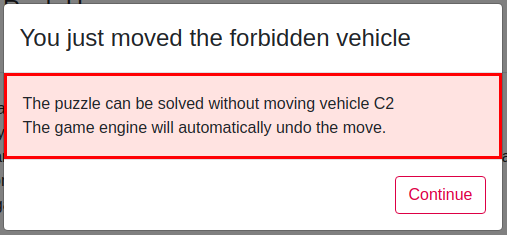
\includegraphics[width=0.5\columnwidth, keepaspectratio=true]{img/badcaralert.png}
  \caption{Forbidden vehicle move alert message}
  \label{fig:badcar}
\end{figure}

\section{Rush Hour Puzzle Design Decisions}
When choosing Rush Hour puzzle configurations for the study, we want to carefully balance the puzzle's difficulty considering a human user. 
Especially, given the PSPACE-completeness of the (generalized) puzzle, we need the puzzles to be solvable by human users in a reasonable time. 
Further, we use the Rush Hour puzzle as a supplementary task comparable to human users learning to use a new software or a web application. 
Therefore, the puzzle solving task should pose a sufficient challenge for the user during the search for a solution in order to make the intervention step more meaningful. We introduce a forbidden vehicle to restrict the moves the user is allowed to make. 
This is an alternative way to increase the difficulty of the puzzle without having to increase the number of vehicles on the board \cite{fernau2003} to make the puzzle more challenging.
In order to further instill the importance of avoiding the forbidden vehicle in the user's mind, we also provide warning messages on the Web interface (Figure~\ref{fig:ui2}) to inform the user about the presence of a forbidden vehicle and what would happen if the forbidden car was moved. 

Recall that in Chapter~\ref{chap:ch5}, Section~\ref{sec:experimentprotocol1}, we discussed three types of Rush Hour puzzles based on the position of the forbidden vehicle (\textbf{E}dge, \textbf{M}iddle, \textbf{C}orner).
In the first round, where the human subjects solve the puzzle without Human-aware Intervention, we use 10 puzzles.
The Human-aware Intervention learned models are developed using the data collected from the 10 puzzles.
In the second round, where the human subjects solve the puzzle with Human-aware Intervention, we use 13 puzzles.
Table~\ref{tab:puzzles} show the puzzle distribution.
We added three extra puzzles to category M to resolve the distribution imbalance in the first round.
We expect that these three classes of  Rush Hour puzzles will pose unique challenges for the human user when trying to avoid the forbidden vehicle.
\begin{center}
\begin{table}
\begin{tabular}{ll}
\begin{tabular}{|c|c|}
\hline
Type & Puzzles\\
\hline
C & P2, P4, P6, P8 \\
\hline
E & P1, P3, P5, P9, P10 \\
\hline
M & P7 \\
\hline
\end{tabular}
\quad
\begin{tabular}{|c|c|}
\hline
Type & Puzzles\\
\hline
C & P2, P4, P6, P8 \\
\hline
E & P1, P3, P5, P9, P10 \\
\hline
M & P7, P11, P12, P13 \\
\hline
\end{tabular}
\end{tabular}
\caption{Rush Hour puzzles used for the experiment without Human-aware Intervention (left) and with Human-aware Intervention (right)}\label{tab:puzzles}
\end{table}
\end{center}
\begin{figure}[tpb]
  \centering
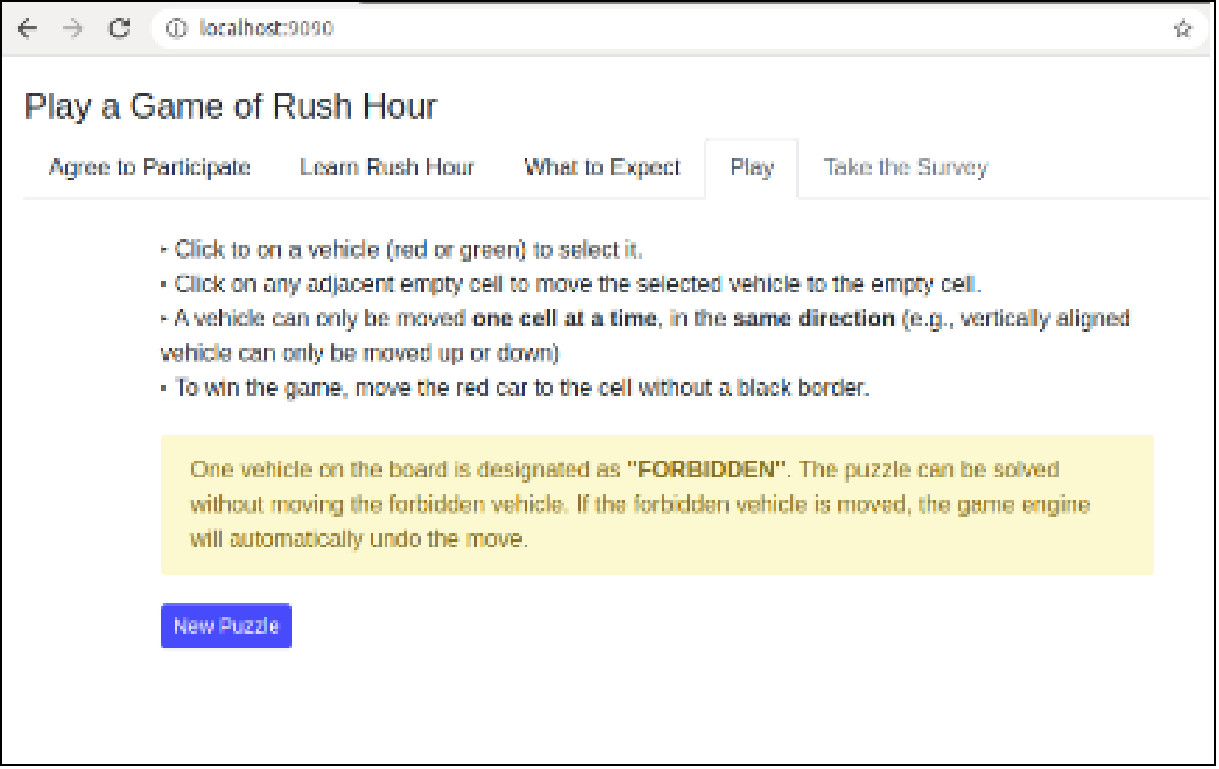
\includegraphics[width=\columnwidth]{img/UI2.pdf}
  \caption{Message about the forbidden vehicle in the Rush Hour planning task}
  \label{fig:ui2}
\end{figure}


\subsection{The Rush Hour Web Simulator}
We designed the Rush Hour software framework to conduct human subject studies in an environment that allows the user to be engaged in a cognitively taxing task. 
The user interacts with several components of the Rush Hour Web Simulator:
\begin{itemize}
\item The consent agreement
\item The Rush Hour tutorial
\item The example solution video
\item The Rush Hour solver (game board)
\item The Post-study survey/debriefing
\end{itemize} 
The components are displayed as tabs on the web page.
If the Rush Hour planning task is solved with the Human-aware Intervention and the hints, then the human user can also view an example solution video that shows how to solve the puzzle without moving the forbidden vehicle.
The example solution video is shown before the actual puzzle solving task begins.
The Rush Hour solver component allows the user to start a puzzle solving task by clicking a button. 
Then a random Rush Hour puzzle is fetched from the server. 
The participant can move the vehicles on the board by clicking once on the vehicle to select it and then clicking once on an adjacent empty cell to move it to that cell. 
To comply with the classical planning model that uses discrete actions, the web application forces the user to move the vehicles one cell at a time.
All illegal moves are blocked and the user is alerted if the he attempts to make an illegal move.
\begin{figure}[tpb]
  \centering
  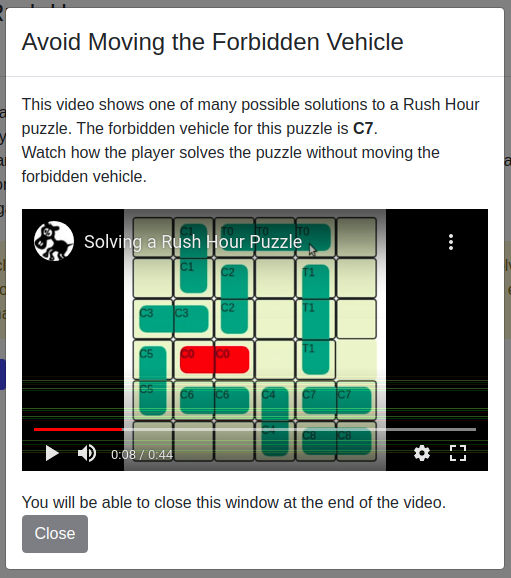
\includegraphics[width=0.6\columnwidth, keepaspectratio=true]{img/help.png}
  \caption{Rush Hour example solution video}
  \label{fig:video}
\end{figure}

\subsection{System Design Decisions}
We design the Rush Hour software framework to conduct human subject studies in an environment that allows the user to be engaged in a cognitively taxing task. 
Our first design choice was in establishing the physical setup of the system. 
Because the experiments are targeted toward all kinds of computer software users (experts/non-experts), we wanted the subjects' attention to be mainly on the puzzle solving task and not be distracted by a complex user-interface. 
To allow for more users to participate, while minimizing the time commitment and the effort, we wanted the system to be accessible from anywhere (e.g, home, university). 
Because of these reasons we designed the system to be a single page web application.

Our next design decision is concerned with capturing and storing experiment data. 
As per the university Institutional Review Board (IRB) regulations, the subject data is required to be stored in a secure manner. 
Further, because our system is deployed as a web application, multiple users may use the system at once and we need to ensure the data is transferred from the web application client to the server securely. 
We established communication between the client and the server over HTTPS via a stateless request-response scheme. 
The client side uses NodeJS, an asynchronous, event-driven JavaScript run-time, which is designed to build scalable network applications.  
The client also uses NodeJS security modules (Helmet) for improved security. 
The data is stored in a secure remote, server dedicated to the web application. 

Our third design decision concerns with the interactivity of the system components.
The design of the system needs to facilitate seamless transition between the two operating modes: learning behavior patterns that can be used as indicators of users' needing help and evaluating learned intervention models in situ. 
Therefore,  we designed the web application to interact with micro-services via a RESTful API. 
Our system architecture is RESTful, in the sense that the client interacts with the server by sending HTTP GET and POST requests using JSON messages to an endpoint URL in the server. 
The API defines many services (persisting game state, intervention, providing hints etc.). 
These services are implemented as separate components on the server. 
REST API response payloads sent from the server are text and encoded in JSON. The response is parsed at the client and appropriate event is triggered on the user interface. 
In addition to supporting platform-independence, which encourages user participation, the services can be activated and deactivated based on the operational mode. 
This allows us to extend the existing system to evaluate how human users respond different intervention models in the future.


\subsection{System Architecture}
The basic system architecture is a JavaScript single page web application in an HTML5 browser that uses RESTful API to access micro-services provided by a Java server running on Linux. 
The client consists of a minimal \texttt{index.html} file that loads and executes the bundled JavaScript application. 
The client and server files are bundled into a single JAR file for the execution on the Linux server at a specified port. 
Figure~\ref{fig:architecture} illustrates the system architecture.

\begin{figure}[tpb]
  \centering
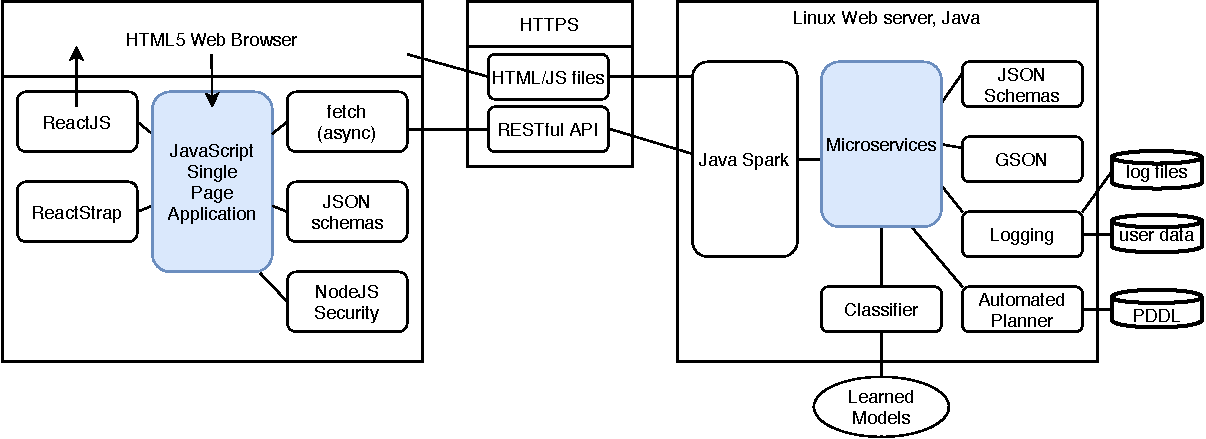
\includegraphics[width=\columnwidth]{img/architecture.pdf}
  \caption{The client-server architecture of the Rush Hour Web Simulator}
  \label{fig:architecture}
\end{figure}

The system is a client-server application that communicates over HTTPS. 
On the client side, the browser loads the \texttt{index.html} file, which in turn loads the bundled JavaScript single page application \texttt{bundle.js}. 
The single page application makes RESTful API requests to the server on the same port using JavaScript's asynchronous fetch. 
We defined several JSON schema to enable message passing between the client and the server via the RESTful API. 
The JSON schema verify requests on the server side and responses on the client side. 
Any verification failures are handled by error responses, also defined in the JSON schema. 
ReactJS renders the application using ReactStrap on the client. 
Because the communication between the client and the server occurs over the Internet, we use the NodeJS security module Helmet to secure the HTTP headers to prevent attacks like cross-site scripting.

On the server side, GSON is used to convert the JSON requests from the client to Java objects and Java objects to JSON responses. 
The server uses Java logging to record user data (moves, survey responses on the client side) and errors that occur on the server side on text files. 
The component that contains the learned model, which implements Human-aware Intervention and the automated planner components are activated only when the system is used to evaluate learned intervention models. 
The automated planner component uses PDDL problem and domain definitions to retrieve information about $P_{observer}$ to help guide the user using the hints.

As the subject interacts with each component, unique API calls are triggered to inform the server about the status of the game. 
The consent agreement component lets the subject read the terms and conditions of the study and give informed consent to participate in the study as required by the IRB. 
When the user gives consent to participate in the study, the user gets assigned a unique identifier and components 2 and 3 get activated. 
This unique identifier is maintained at both the client side (as the Local Storage entry in the Web browser) and on a text file at the server until the user's session ends. 
The Rush Hour tutorial presents a brief introduction to the Rush Hour puzzle, the rules and the objective of the puzzle. 
Figure~\ref{fig:ui1} shows the tutorial for the Rush Hour planning task.
It also shows an example play to educate the user on how to select and move objects on the web interface. 
The consent agreement and the tutorial are static components, in the sense the user does not have a lot of flexibility to change the contents through interaction. 
The example solution video allows minimal interaction to pause and replay the solution video.
The video component is only available if the Rush Hour Simulator is operating with the Human-aware Intervention.
On the other hand, the solver is a dynamic and an interactive component. 
The solver component allows the user to start a puzzle solving task by clicking a button, which fetches a random Rush Hour puzzle from the server. 
Figure~\ref{fig:ui3} shows how the puzzle is displayed to the human user.
The participant can move the vehicles on the grid by first clicking once on the vehicle to select it and then clicking once on an adjacent empty cell to move it to the selected cell. To comply with the classical planning model of discrete actions, the application forces the user to move the vehicles one step at a time. 
This rule invalidates moves that jump over multiple cells on the puzzle boards. 
The other illegal move is user attempting to move a vehicle in the opposite orientation. When the user makes one of these illegal moves, error messages are displayed and the move is blocked. 
All legal moves the user make are temporarily kept in in-memory data structures on the client side. 
Once the user finishes the puzzle solving task, an API call is invoked to initiate the data transmission between the client and the server in a secure manner via HTTPS. 
The server records the users solution on a text file in a directory created with the user's identifier. 
When the user's solution is stored on the server successfully, the post-study survey and debriefing component is activated. 
If the Rush Hour Web Simulator operates without the Human-aware Intervention mode, the survey collects demographic data and the user's general puzzle solving habits.
If the Rush Hour Web Simulator operates in the Human-aware Intervention mode, the survey collects participant demographics and a subjective rating on how useful the hints were to the user.
Once the user completes the survey, the data is transmitted to the server and stored as text files.
\begin{figure}[tpb]
  \centering
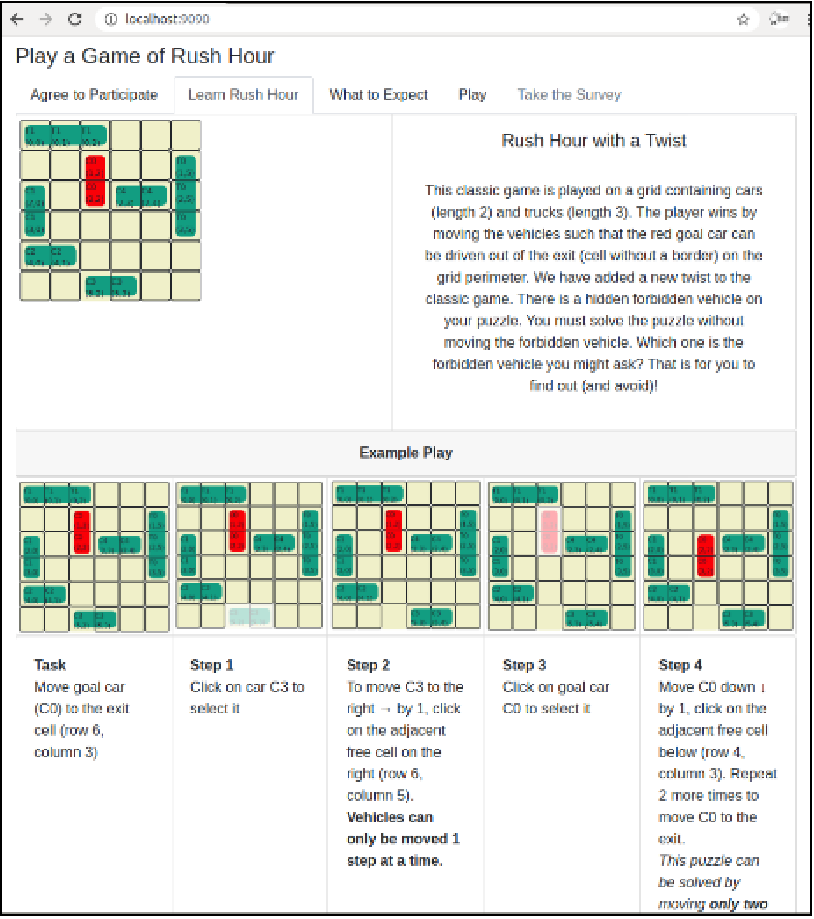
\includegraphics[width=\columnwidth]{img/UI1.pdf}
  \caption{The Rush Hour planning task tutorial}
  \label{fig:ui1}
\end{figure}

\begin{figure}[tpb]
  \centering
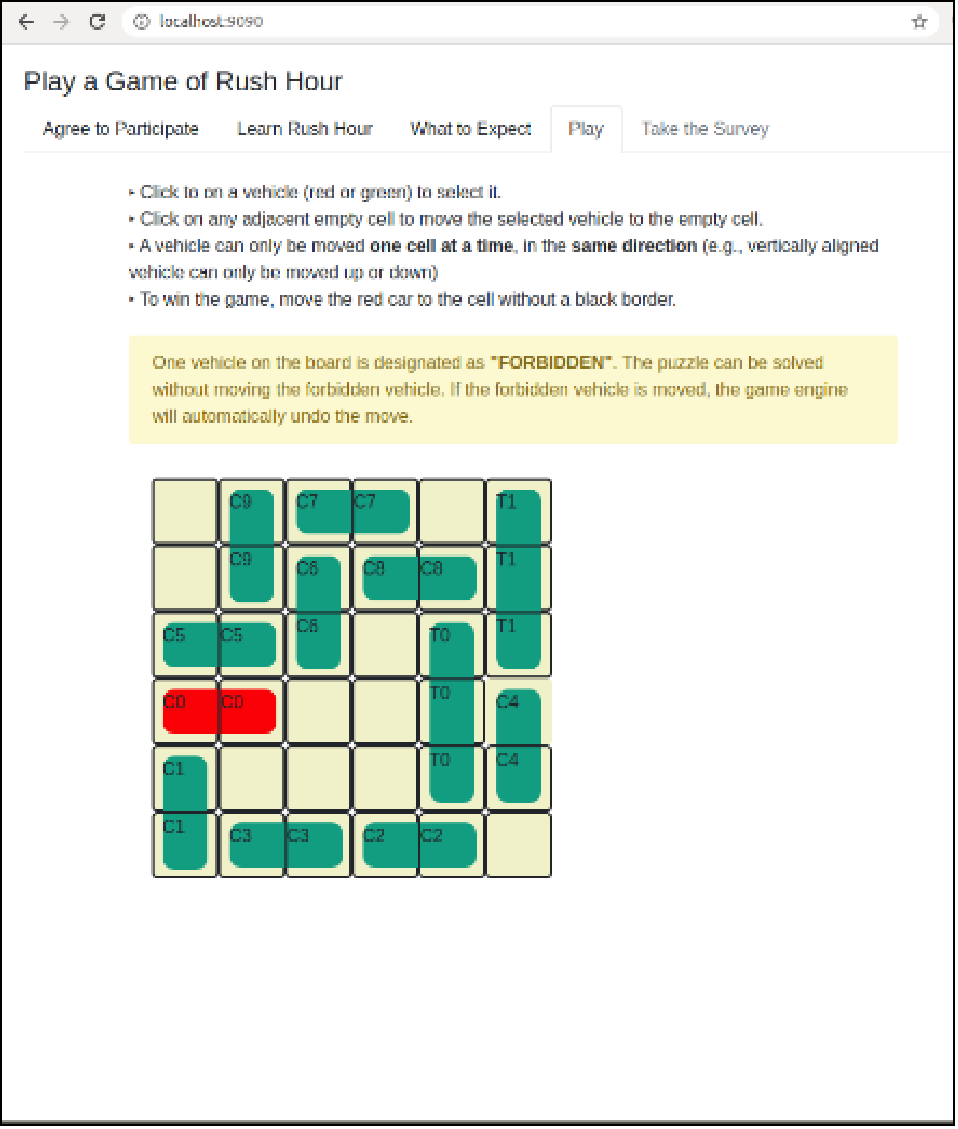
\includegraphics[width=\columnwidth]{img/UI3.pdf}
  \caption{The Rush Hour planning task solver interface}
  \label{fig:ui3}
\end{figure}

\subsection{The Rush Hour Web Simulator - Client-side Operation}
\begin{figure}[tpb]
  \centering
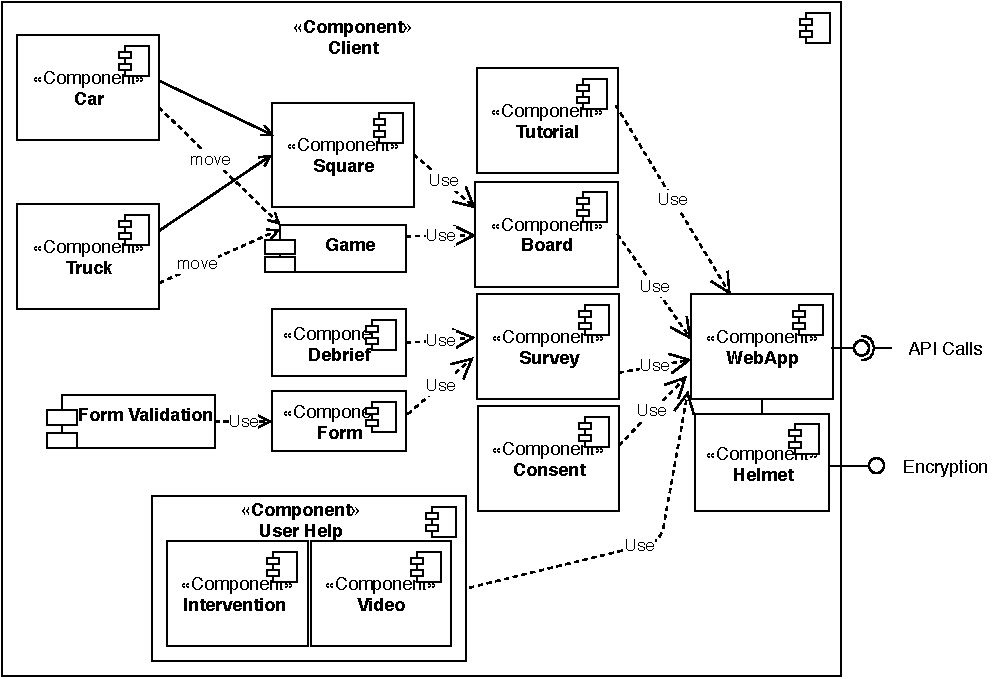
\includegraphics[width=\columnwidth]{img/componentclient.pdf}
  \caption{UML component diagram for the Rush Hour Web Simulator client}
  \label{fig:compclient}
\end{figure}

Figure \ref{fig:compclient} illustrates the component structure of the Rush Hour Web Simulator client.
The \textbf{WebApp} component integrates the sub components: the consent agreement, the Rush Hour tutorial, the Rush Hour solver, the user help and the survey. 
The user help component consists of interactive Human-aware Intervention messaging model (implemented in the \textbf{Intervention} component) and the help video (implemented in the \textbf{Video} component).
The Rush Hour solver (implemented in the \textbf{Board} component) is further broken down in to sub components, which model different objects in the game such as cars, trucks and squares.
The \textbf{Game} component implements the rules of the Rush Hour puzzle.
The \textbf{Survey} component contains two components that implement the debriefing statement and the post study questionnaire.
Each client component communicates using API calls within them.
The WebApp component invokes the API calls on the sever component in the Rush Hour Web Simulator to fetch intervention decisions and log the events that take place on the Web Simulator interface.
When the Human-aware Intervention occurs the Intervention component displays a pop-up message with the hints (Figure~\ref{fig:help} - left).
When the user selects a hint, the client makes another API call to fetch the appropriate property value of the $P_{observer}$ as the response from the server. 
The response is displayed as a follow up dialog box and the user is allowed to continue on with the Rush Hour planning task (Figure~\ref{fig:help} - right). 
\begin{figure}[tpb]
  \centering
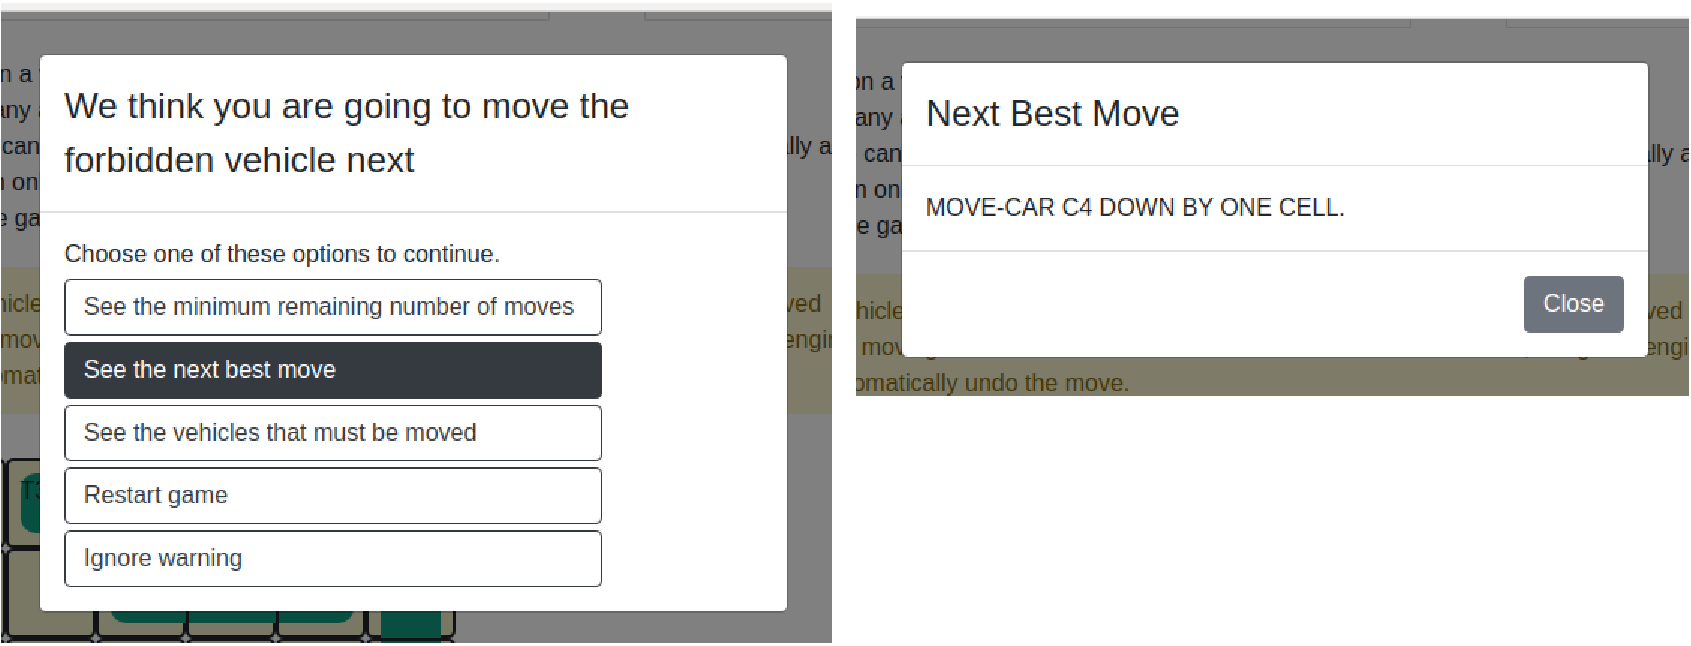
\includegraphics[width=\columnwidth]{img/alert.pdf}
  \caption{Interactive Human-aware Intervention (left) and the hint response (right)}
  \label{fig:help}
\end{figure}
Figure \ref{fig:help} shows the intervention message shown to the user (left) and  the user requesting to see the next best move as the hint. Subsequently, the server responds with the property value of the $P_{observer}$  and the client displays the message on the right.
One of the hint options is to let the user ignore Human-aware Intervention. 
The Intervention component keeps track of how many times the user has chosen to ignore intervention and after two consecutive ignore requests, the client terminates fetching hint responses from the server. 
When the Rush Hour planning task finishes, the user's solution and the Human-aware Intervention decisions received during the planning task are automatically transmitted to the server to be saved as text files.


\subsection{The Rush Hour Web Simulator - Server-side Operation}
As shown in Figure \ref{fig:compserver}, the Rush Hour Web Simulator server responds to client's API calls through the \textbf{MicroServer} component.
The MicroServer consists of messaging frameworks (\textbf{GSON}, \textbf{Spark}, \textbf{JSON}) and message logging (implemented in the \textbf{Logger} component).
In addition, the \textbf{Data Persistence} component supports saving the user solutions, client-side events in text files.
The \textbf{Intervention} component and the \textbf{Planning} component on the server are used to recognize Human-aware Intervention and generate helpful hints respectively. The \textbf{Intervention} component uses a learned Human-aware Intervention model to identify when the user needs help. 
The \textbf{Planning} component generates the responses to the user's hint requests (see Definition~\ref{def:hint}) by solving $P_{observer}$ using an automated planner.
We integrated the Fast Downward planner \cite{helmert2006} to the Planning component to generate cost optimal plan for $P_{observer}$. 
The Fast Downward planner was configured to use the A-star search algorithm with the admissible heuristic Landmark-cut (\texttt{lmcut}) \cite{helmert2009} to find cost optimal plans.
\begin{figure}[tpb]
  \centering
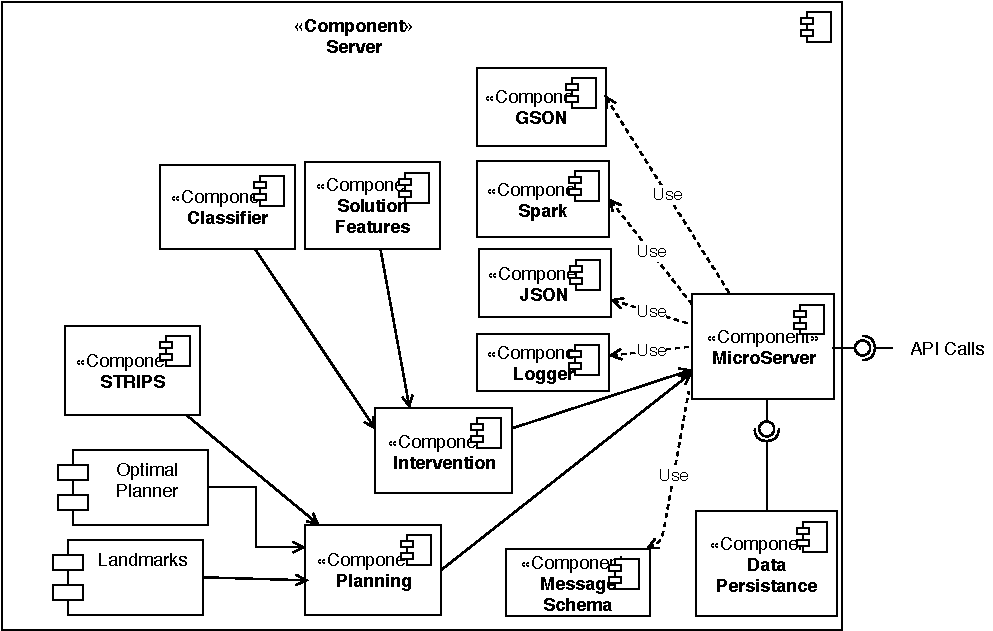
\includegraphics[width=\columnwidth]{img/componentserver.pdf}
  \caption{UML component diagram for the Rush Hour Web Simulator server}
  \label{fig:compserver}
\end{figure}

We use a minimalist and responsive design (supported by \texttt{ReactStrap} library) for the Rush Hour Web Simulator interface to help the user to start the puzzle solving task with a very small learning curve. 
The simple, non-intrusive messaging model we designed for the client-server communication automatically sends the event data back and forth between the client and the server and helps the user focus completely on the puzzle solving task.
The system is deployed on a secure Linux Web server with a public IP address, which allows the users to access the application from anywhere on a variety of devices. 



\section{Experiment Design}
In the first round, the human users solved Rush Hour planning tasks without Human-aware Intervention (see Appendix~\ref{ap:phase1design} for details).
In the second phase, the application intervenes the user and provides helpful hints.
We recruited 142 participants from a university student population.
The participants were not compensated for their time.
Upon agreeing to participate in the study each subject is assigned one puzzle randomly out of 13 puzzles. 
In addition, the participants are randomly selected to watch a 44 second video of a sample game play.
The video showed how a Rush Hour planning task can be solved by avoiding the forbidden vehicle.
All participants had the option to use the only tutorial available on the Rush Hour Web Simulator to learn the rules of the puzzle.
The participants were informed that one of the vehicles on the board is forbidden and the puzzle must be solved without moving it.
During the Rush Hour planning task, the participant is shown the hints when the learned model recognizes that the he/she needs help (see Figure \ref{fig:help}). 
The participant can follow a hint or decide to ignore it.
Based on the user's choice, a second alert message is shown, with the corresponding property of $P_{observer}$. 
Once the puzzle solving task is completed, the participants are asked to complete a short survey to capture the demographics and also asks them to subjectively rate the helpfulness of each hint type on a 5-point Likert scale. 
Figure~\ref{fig:phase2} illustrates the activity sequence of the experiment.
\begin{figure}[tpb]
  \centering
  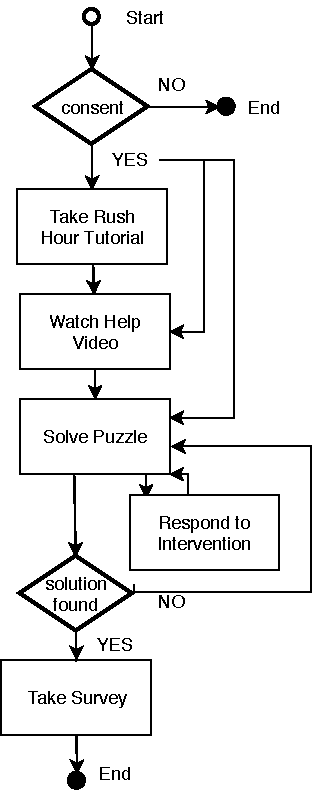
\includegraphics[height=0.6\columnwidth]{img/phase2.pdf}
  \caption{Activity sequence for evaluating hints during intervention for the Rush Hour human subject experiment}
  \label{fig:phase2}
\end{figure}

\subsection{Collecting Data}
From the 142 participants, we removed records of 7 subjects because they had quit the session before the Rush Hour planning task was completed. 
The remaining 135 records are used in the evaluation.
130 of the 135 participants also completed the post-study survey.
For each participant, we record the solution, requested hints, the demographic information and the 5-point helpfulness rating for the hints.

\section{Results and Evaluation}
We first present the findings of the post-study survey, discuss the properties of our study sample and outline how human users subjectively rated the helpfulness of the hints.
Next, we turn our attention to the solutions produced by human users under two experimental conditions.
As the first experimental condition, the human users solved Rush Hour planning tasks without hints.
We refer to the first group as the \textbf{control group}.
We discussed the findings of this study in Chapter~\ref{chap:ch5}.
In this chapter, we discuss the findings of the second experimental condition where the human users solved the Rush Hour planning tasks with hints.
We refer to the second group as the \textbf{condition group}.
Therefore, we have a between group experimental design to evaluate the effect of using hints between the control and the condition group.
We present the summary statistics for the number of moves in the solutions in the control and the condition groups and compare the solutions that moved the forbidden vehicle and the solutions that did not.
Next we compare the

\subsection{Findings of the Post-study Survey}
From the 131 participants who completed the demographics survey, the majority (52) were between the age of 20 - 25. 
There were 51 participants whose age was less than 20 years. 
Additionally, there were 12 participants each from 31 - 25 age group and 26 - 30 age group. 
There was 1 participant in the 36 - 40 age group. 
Two participants were above the age of 41.
We were able to recruit participants from different educational backgrounds.
As illustrated in Figure~\ref{fig:demophase2}, the majority of the participants (27) are Business majors, followed by Animal Sciences (14) and Arts and Humanities (10).
47\% of the participants have seen the Rush Hour puzzle before.
\begin{figure}[tpb]
  \centering
  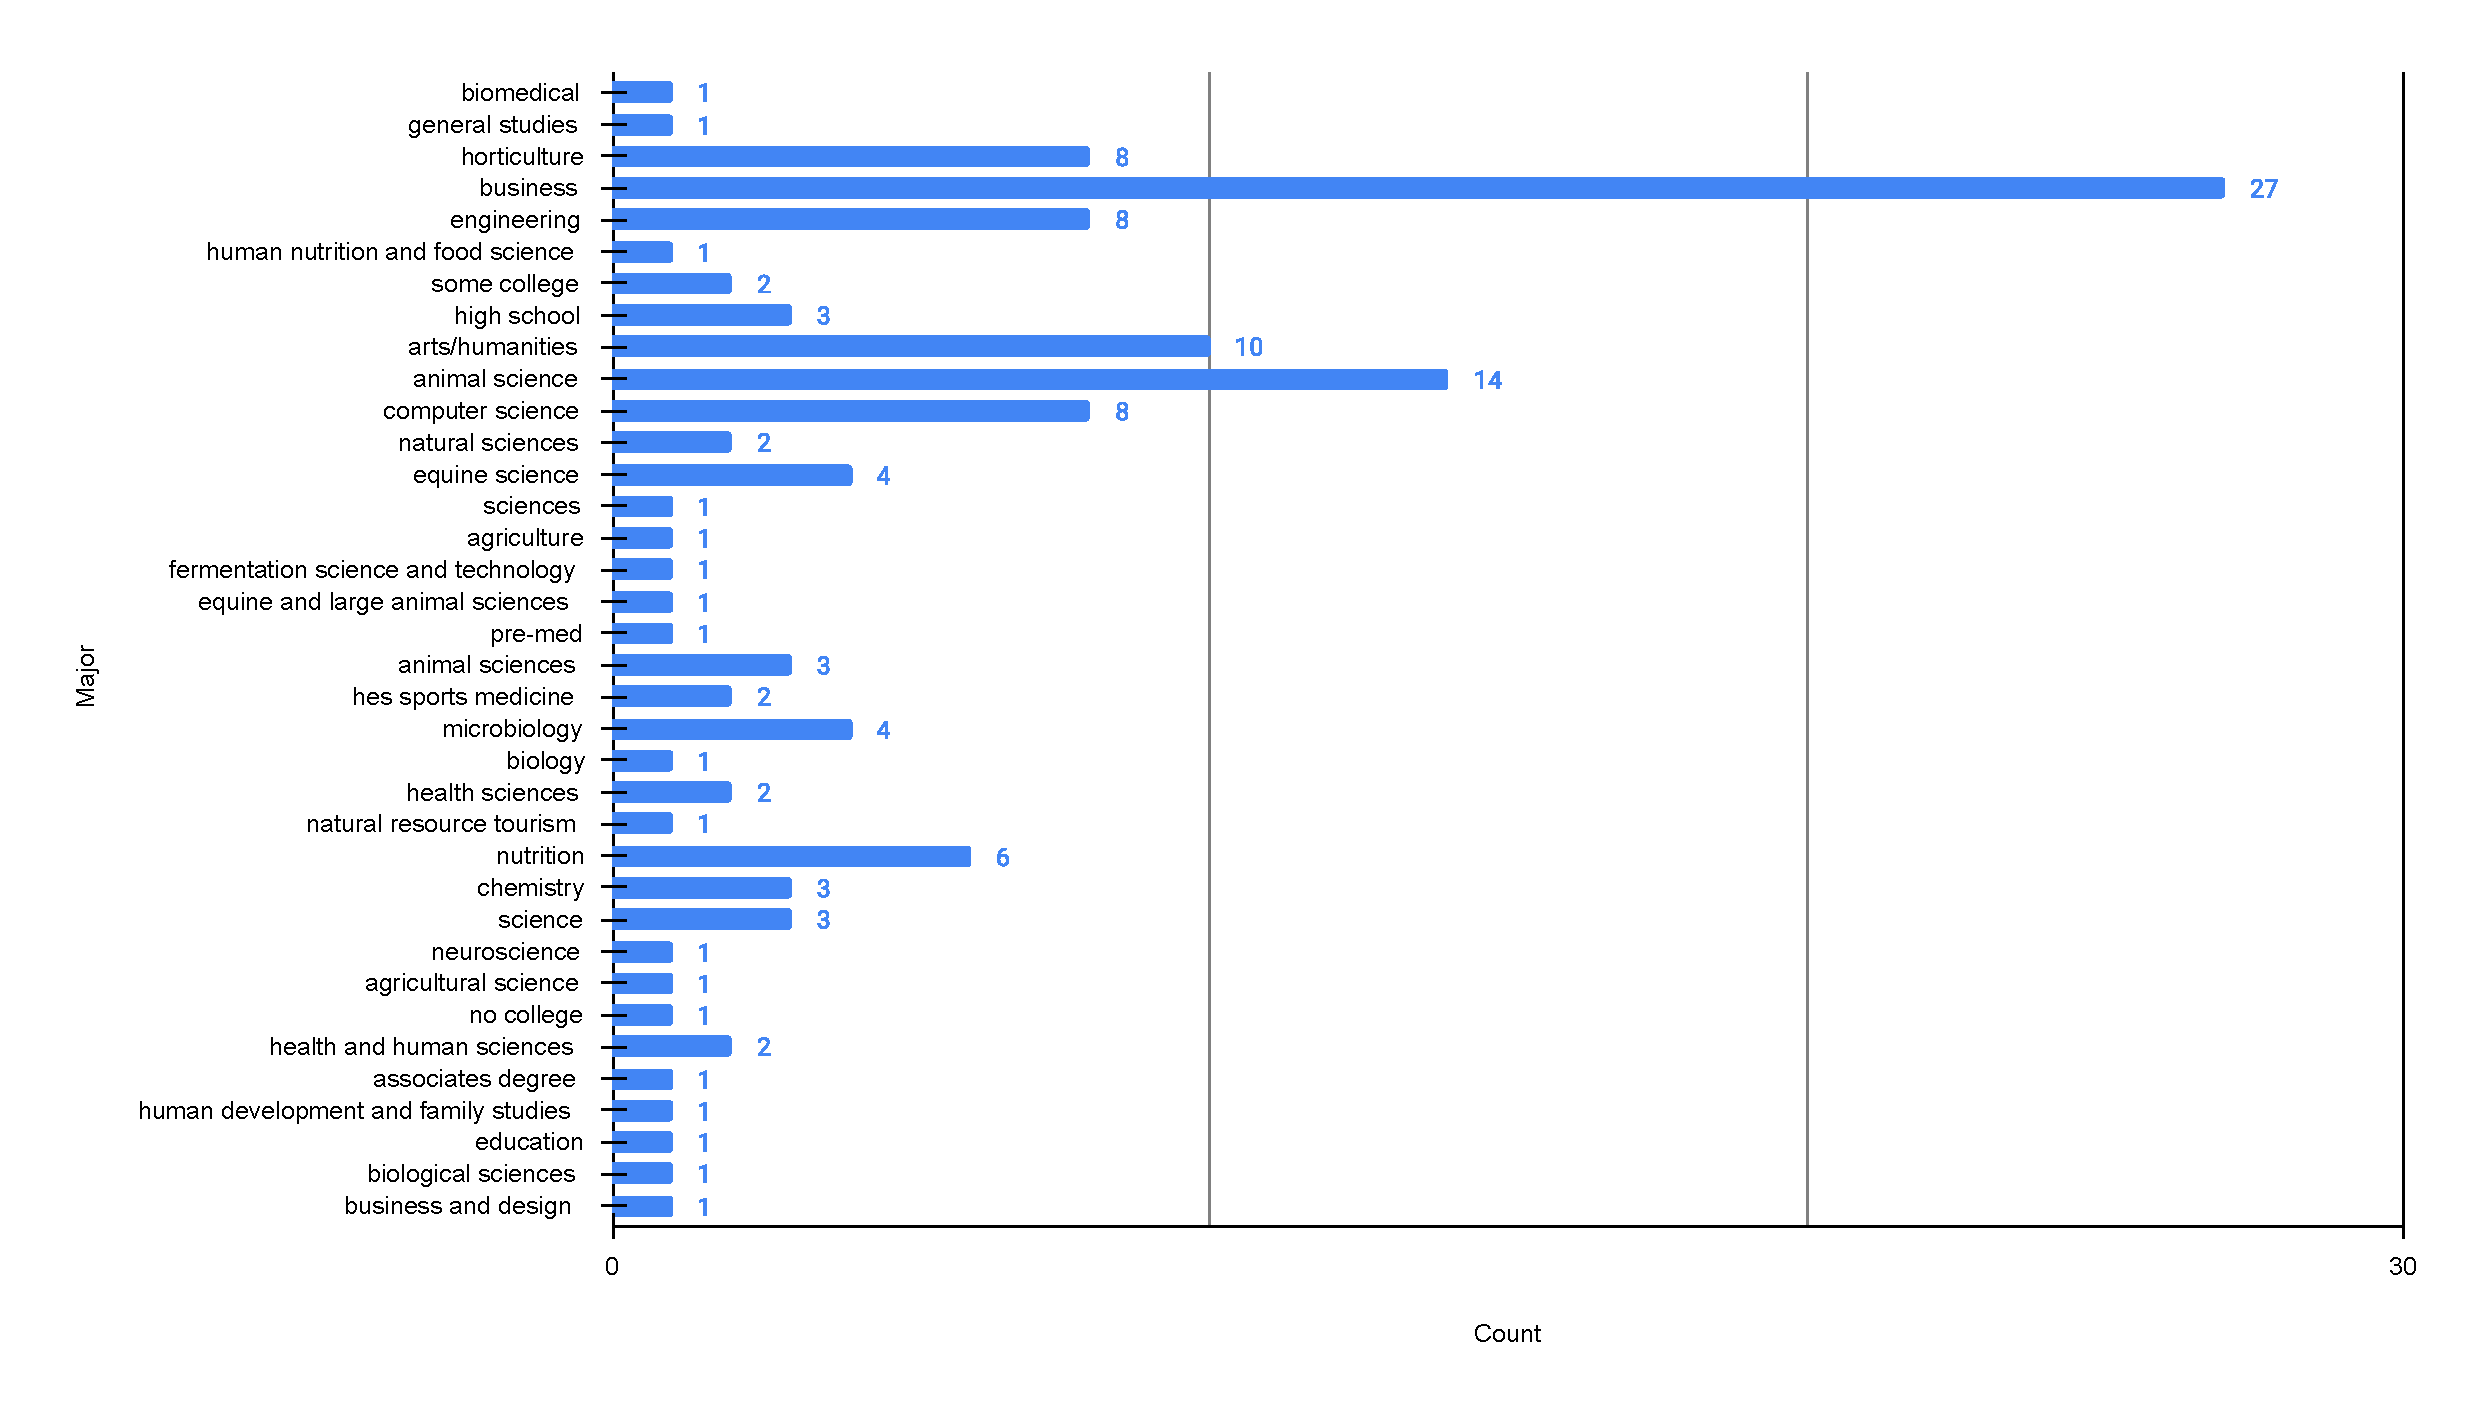
\includegraphics[height=0.6\columnwidth]{img/demophase2.pdf}
  \caption{Educational backgrounds of the study participants}
  \label{fig:demophase2}
\end{figure}

From the 135 participants who completed the Rush Hour planning task, 44 subjects did not use any hints. 
From the remaining 91 participants, 4 subjects did not complete the demographics survey.
So we were unable to collect demographic data on them.
We also asked the participants to rate the hints in 5 point rating scale (1 being the lowest rating and 5 being the highest) based on how helpful the hints were in helping them avoid the forbidden vehicle.
Table~\ref{tab:phase2ratings} summarizes the mean and the standard deviation of the subjective ratings.
It can be seen that across all three puzzle types,  the hint ``\textbf{Show the next best move}'' has the highest subjective helpfulness rating.
This indicates that when human users are stuck during the Rush Hour planning task (i.e., getting close to moving the forbidden vehicle) they subjectively prefer information that tells directly them what to do next.
Considering the puzzle types C, E and M, we could not find unique subsets of hints the participants preferred the most.

\begin{table}[tbp]
\begin{tabular}{lll|l|l|l|l|}
\cline{4-7}
 &  &  & \multicolumn{4}{l|}{\textbf{Mean (std. dev.) helpfulness rating}} \\ \hline
\multicolumn{1}{|l|}{\textbf{Type}} & \multicolumn{1}{l|}{\textbf{Puzzle ID}} & \textbf{Count} & \multicolumn{1}{c|}{H1} & \multicolumn{1}{c|}{H2} & \multicolumn{1}{c|}{H3} & \multicolumn{1}{c|}{H4} \\ \hline
\multicolumn{1}{|c|}{\multirow{4}{*}{\textbf{C}}} & \multicolumn{1}{l|}{P2} & 6 & 1.5 (2.5) & 4.3 (2.6) & 3.8 (2.3) & 2.0 (2.3) \\
\multicolumn{1}{|c|}{} & \multicolumn{1}{l|}{P4} & 11 & 1.3 (2.1) & 2.3 (2.1) & 1.5 (2.2) & 0.8 (1.7) \\
\multicolumn{1}{|c|}{} & \multicolumn{1}{l|}{P6} & 3 & 2.0 (1.2) & 3.3 (2.6) & 1.7 (2.9) & 0 \\
\multicolumn{1}{|c|}{} & \multicolumn{1}{l|}{P8} & 1 & 0 & 3.0 & 3.0 & 1.0 \\ \hline
\multicolumn{1}{|l|}{\multirow{5}{*}{\textbf{E}}} & \multicolumn{1}{l|}{P1} & 4 & 1.5 (1.3) & 4.3 (1.0) & 3.8 (1.9) & 2.0 (2.2) \\
\multicolumn{1}{|l|}{} & \multicolumn{1}{l|}{P3} & 13 & 1.3 (1.6) & 2.3 (2.2) & 1.5 (1.7) & 0.8 (0.9) \\
\multicolumn{1}{|l|}{} & \multicolumn{1}{l|}{P5} & 13 & 1.4 (1.3) & 2.2 (1.9) & 2.2 (2.0) & 1.8 (1.9) \\
\multicolumn{1}{|l|}{} & \multicolumn{1}{l|}{P9} & 7 & 0.9 (1.2) & 1.7 (2.2) & 1.1 (1.7) & 1.3 (2.0) \\
\multicolumn{1}{|l|}{} & \multicolumn{1}{l|}{P10} & 8 & 0.9 (1.0) & 2.8 (2.3) & 1.6 (1.5) & 2.8 (2.1) \\ \hline
\multicolumn{1}{|l|}{\multirow{4}{*}{\textbf{M}}} & \multicolumn{1}{l|}{P7} & 6 & 2.0 (2.1) & 3.5 (2.1) & 2.5 (1.9) & 1.8 (1.3) \\
\multicolumn{1}{|l|}{} & \multicolumn{1}{l|}{P11} & 3 & 2.0 (2.6) & 3.3 (2.9) & 2.0 (2.6) & 3.3 (2.9) \\
\multicolumn{1}{|l|}{} & \multicolumn{1}{l|}{P12} & 1 & 1.0 & 5.0 & 5.0 & 1.0 \\
\multicolumn{1}{|l|}{} & \multicolumn{1}{l|}{P13} & 11 & 1.2 (1.8) & 1.7 (1.8) & 0.9 (1.4) & 0.9 (1.6) \\ \hline
\end{tabular}
\caption{Mean (standard deviation) of the subjective helpfulness rating the subjects assigned for the hints \textbf{H1}: Show the minimum remaining number of moves, \textbf{H2}: Show the next best move, \textbf{H3}: Show the vehicles that must be moved, \textbf{H4}: restart puzzle}
\label{tab:phase2ratings}
\end{table}

\subsection{Safe and Unsafe Solutions in the Control and the Condition Groups}
We now compare the solution lengths of the control and the condition groups by breaking each group's solutions into two types: safe and unsafe. 
We refer to solutions that did not move the forbidden vehicle as \textbf{safe} and solutions that moved the forbidden vehicle as \textbf{unsafe}.
In the control group, 66 users from the total 136 produced solutions that involved moving the forbidden vehicle (49\%).
From those who moved the forbidden vehicle, 54 users moved the vehicle more than once (82\%).
Table \ref{tab:usersolutions} describes the summary statistics for the solutions that did not move the forbidden vehicle and the solutions that moved the forbidden vehicle produced by the human users in the control group.

\begin{table}[tpb]
\begin{tabular}{|l|l|l|l|l|l|l|l|l|l|l|}
\hline
\multicolumn{1}{|c|}{\multirow{2}{*}{PID}} &
  \multicolumn{5}{c|}{Safe Solutions} &
  \multicolumn{5}{c|}{Unsafe Solutions} \\ \cline{2-11} 
\multicolumn{1}{|c|}{} &
  \multicolumn{1}{c|}{Freq} &
  \multicolumn{1}{c|}{Min} &
  \multicolumn{1}{c|}{Max} &
  \multicolumn{1}{c|}{Mean} &
  \multicolumn{1}{c|}{Std. dev.} &
  \multicolumn{1}{c|}{Freq} &
  \multicolumn{1}{c|}{Min} &
  \multicolumn{1}{c|}{Max} &
  \multicolumn{1}{c|}{Mean} &
  \multicolumn{1}{c|}{Std. dev.} \\ \hline
P1  & 18 & 24 & 106 & 43.9  & 20.5  & -  & -  & -   & -    & -    \\ 
P2  &  3  & 44 & 158 & 99.3 & 57.1 & 8  & 78 & 378 & 190.3 & 120.0\\ 
P3  & -  & -  & -   & -     & -     & 12 & 25 & 50  & 35.5 & 8.3  \\ 
P4  & 9  & 23 & 46  & 30    & 7.1   & 7  & 25 & 124 & 67.4 & 33.9 \\ 
P5  & 4  & 23 & 32  & 26.5  & 3.9   & 7  & 14 & 82  & 32.0 & 23.3 \\
P6  & 14 & 22 & 55  & 29    & 10.3  & -  & -  & -   & -    & -    \\
P7  & 2  & 29 & 37  & 33    & 5.7   & 9  & 43 & 132 & 80.9 & 38.2 \\ 
P8  & 18 & 9  & 12  & 9.3   & 0.8   & -  & -  & -   & -    & -    \\
P9  & 2  & 21 & 27  & 24    & 4.2   & 14 & 29 & 169 & 66.3 & 39.0 \\
P10 & -  & -  & -   & -     & -     & 9  & 44 & 158 & 81.2 & 39.2 \\ \hline
\end{tabular}
\caption{Frequency, minimum, maximum, mean and std. deviation number of moves in users' solutions for the Rush Hour planning tasks P1 through P10 \textbf{solved without using hints}}
\label{tab:usersolutions}
\end{table}

In the condition group 44 subjects did not use any hints.
This is because the Human-aware Intervention agent did not classify the partial solutions they were producing as requiring intervention.
Therefore, we only use the data from 91 subjects who solved Rush Hour planning tasks with hints for the analysis. 
Table \ref{tab:usersolutionsphase2} describes the summary statistics for the solutions in the condition group.
65 users from the sample of 91 solved the planning task but failed to avoid the forbidden vehicle (71\%).
In general, where there are a set of safe and unsafe solutions for a given planning task, it can be seen that the mean solution length for the unsafe set is longer than the mean of the unsafe set.
This indicates that the longer the human user spends searching for the solution, the more likely he will move the forbidden vehicle.
There are several similarities between the solution lengths for planning tasks in the control and the condition groups.
First, the planning task P1 did not produce any unsafe solutions for both groups.
The reason for this observation is that when examining the structure of P1 it can be seen that moving the forbidden vehicle makes the planning task unsolvable.
Second, the planning task P8 did not produce any unsafe solutions for both groups.
Furthermore, P8 was the only planning task in type C planning task that did not produce any unsafe solutions.
Third, in both groups, human users found it difficult to avoid the forbidden car for type E planning tasks, where the forbidden car was positioned along the edge of the board.
For type E planning tasks (P3, P5, P9, P10), there are more unsafe solutions than safe solutions and also the mean solution length for unsafe solutions is larger compared to the safe solutions mean.
We did not find a common pattern for the solutions generated by type M planning tasks.
We only had 1 planning task for type M (P7) in the control group.
We had four planning tasks of the same type (P7, P11, P12, P13) in the condition group.
The users in the control group difficult to solve P7 without moving the forbidden vehicle.
In contrast, the solutions generated by the users in the condition group for P7 were evenly split between the safe and unsafe groups.
The same can be observed for puzzle P13.
Figure \ref{fig:phase1split} illustrates the percentage split between unsafe and safe solutions for the control group. 
Figure \ref{fig:phase2split} illustrates the percentage split for the condition group. 

\begin{table}[tpb]
\begin{tabular}{|l|l|l|l|l|l|l|l|l|l|l|}
\hline
\multirow{2}{*}{PID} & \multicolumn{5}{c|}{Safe Solutions}  & \multicolumn{5}{c|}{Unsafe Solutions} \\ \cline{2-11} 
                     & Freq. & Min & Max & Mean & Std. dev. & Freq.  & Min & Max & Mean  & Std. dev \\ \hline
P1                   & 4     & 51  & 80  & 59.7 & 13.7      & -      & -   & -   & -     & -        \\
P2                   & -     & -   & -   & -    & -         & 8      & 67  & 419 & 157.1 & 114.3    \\
P3                   & 1     & 51  & 51  & 51   & -         & 12     & 43  & 121 & 71.8  & 24.8     \\
P4                   & 2     & 34  & 78  & 56   & 31.1      & 9      & 27  & 87  & 55.1  & 19.7     \\
P5                   & 5     & 27  & 49  & 37.6 & 9.5       & 9      & 34  & 154 & 54.9  & 37.7     \\
P6                   & 2     & 34  & 45  & 39.5 & 7.8       & 1      & 62  & 62  & 62    & -        \\
P7                   & 3     & 27  & 59  & 39   & 17.4      & 3      & 44  & 195 & 98.7  & 83.7     \\
P8                   & 1     & 14  & 14  & 14   & -         & -      & -   & -   & -     & -        \\
P9                   & -     & -   & -   & -    & -         & 7      & 22  & 71  & 43.7  & 19.2     \\
P10                  & -     & -   & -   & -    & -         & 8      & 46  & 74  & 58.4  & 9.8      \\
P11                  & 1     & 61  & 61  & 61   & -         & 2      & 50  & 95  & 72.5  & 31.8     \\
P12                  & 1     & 41  & 41  & 41   & -         & -      & -   & -   & -     & -        \\
P13                  & 6     & 24  & 40  & 29.5 & 6.3       & 6      & 30  & 55  & 41.2  & 9.6      \\ \hline
\end{tabular}
\caption{Frequency, minimum, maximum, mean and std. deviation number of moves in users' solutions for the Rush Hour planning tasks P1 through P13 \textbf{solved using hints}}
\label{tab:usersolutionsphase2}
\end{table}

\begin{figure}[tpb]
\centering
	\begin{minipage}[b]{0.45\columnwidth}
	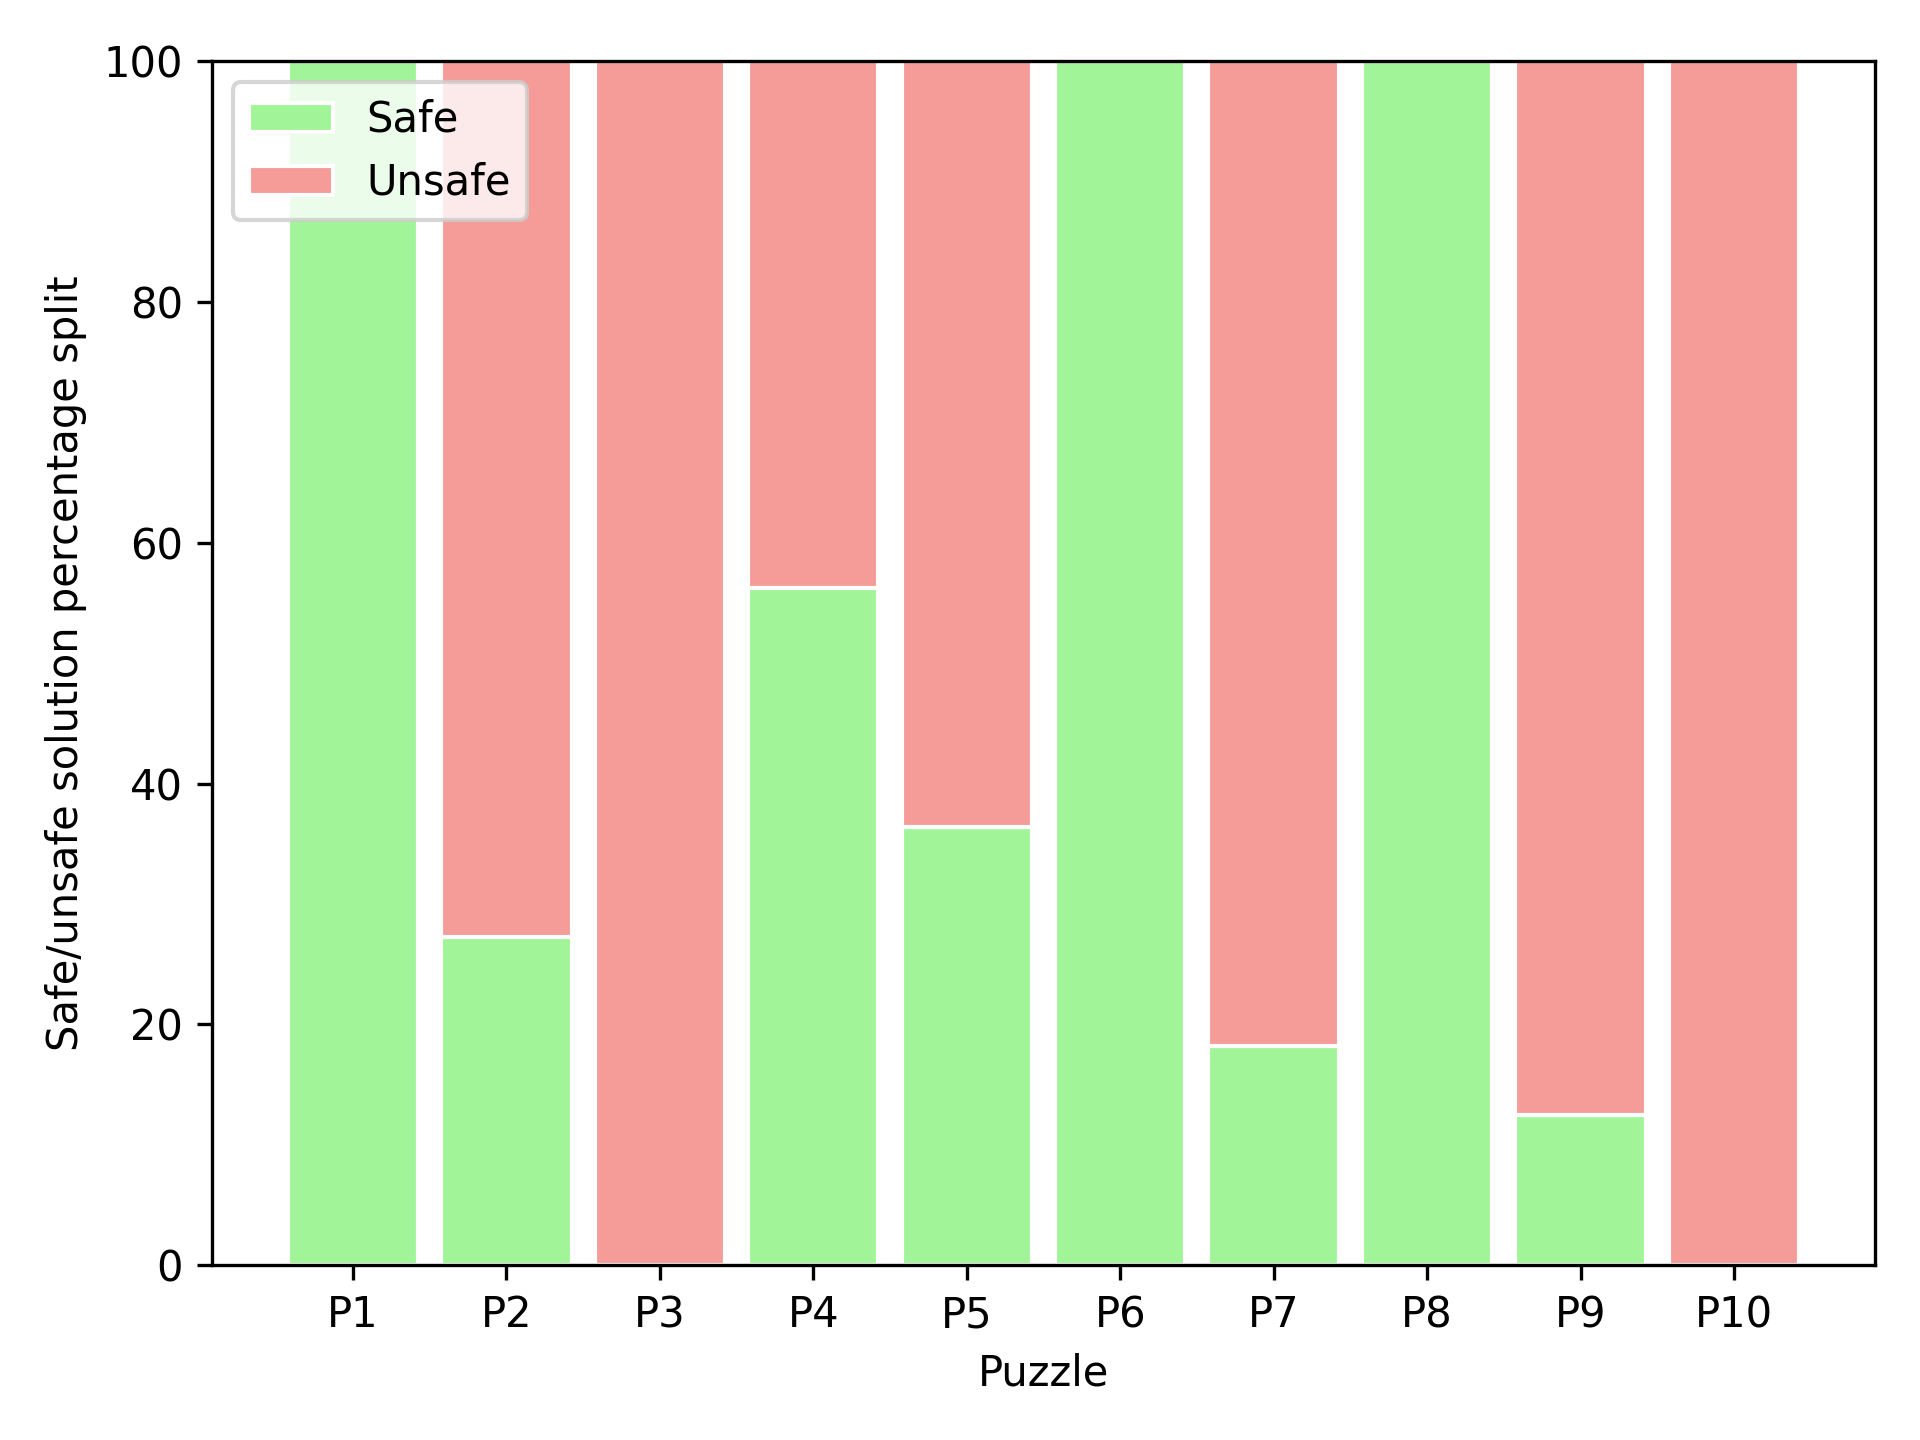
\includegraphics[width=\columnwidth]{img/phase1split.png}
	\caption{Rush Hour planning tasks used in Human-aware Intervention \textbf{without hints}}				
	\label{fig:phase1split}
	\end{minipage}
	\quad
	\begin{minipage}[b]{0.45\columnwidth}
	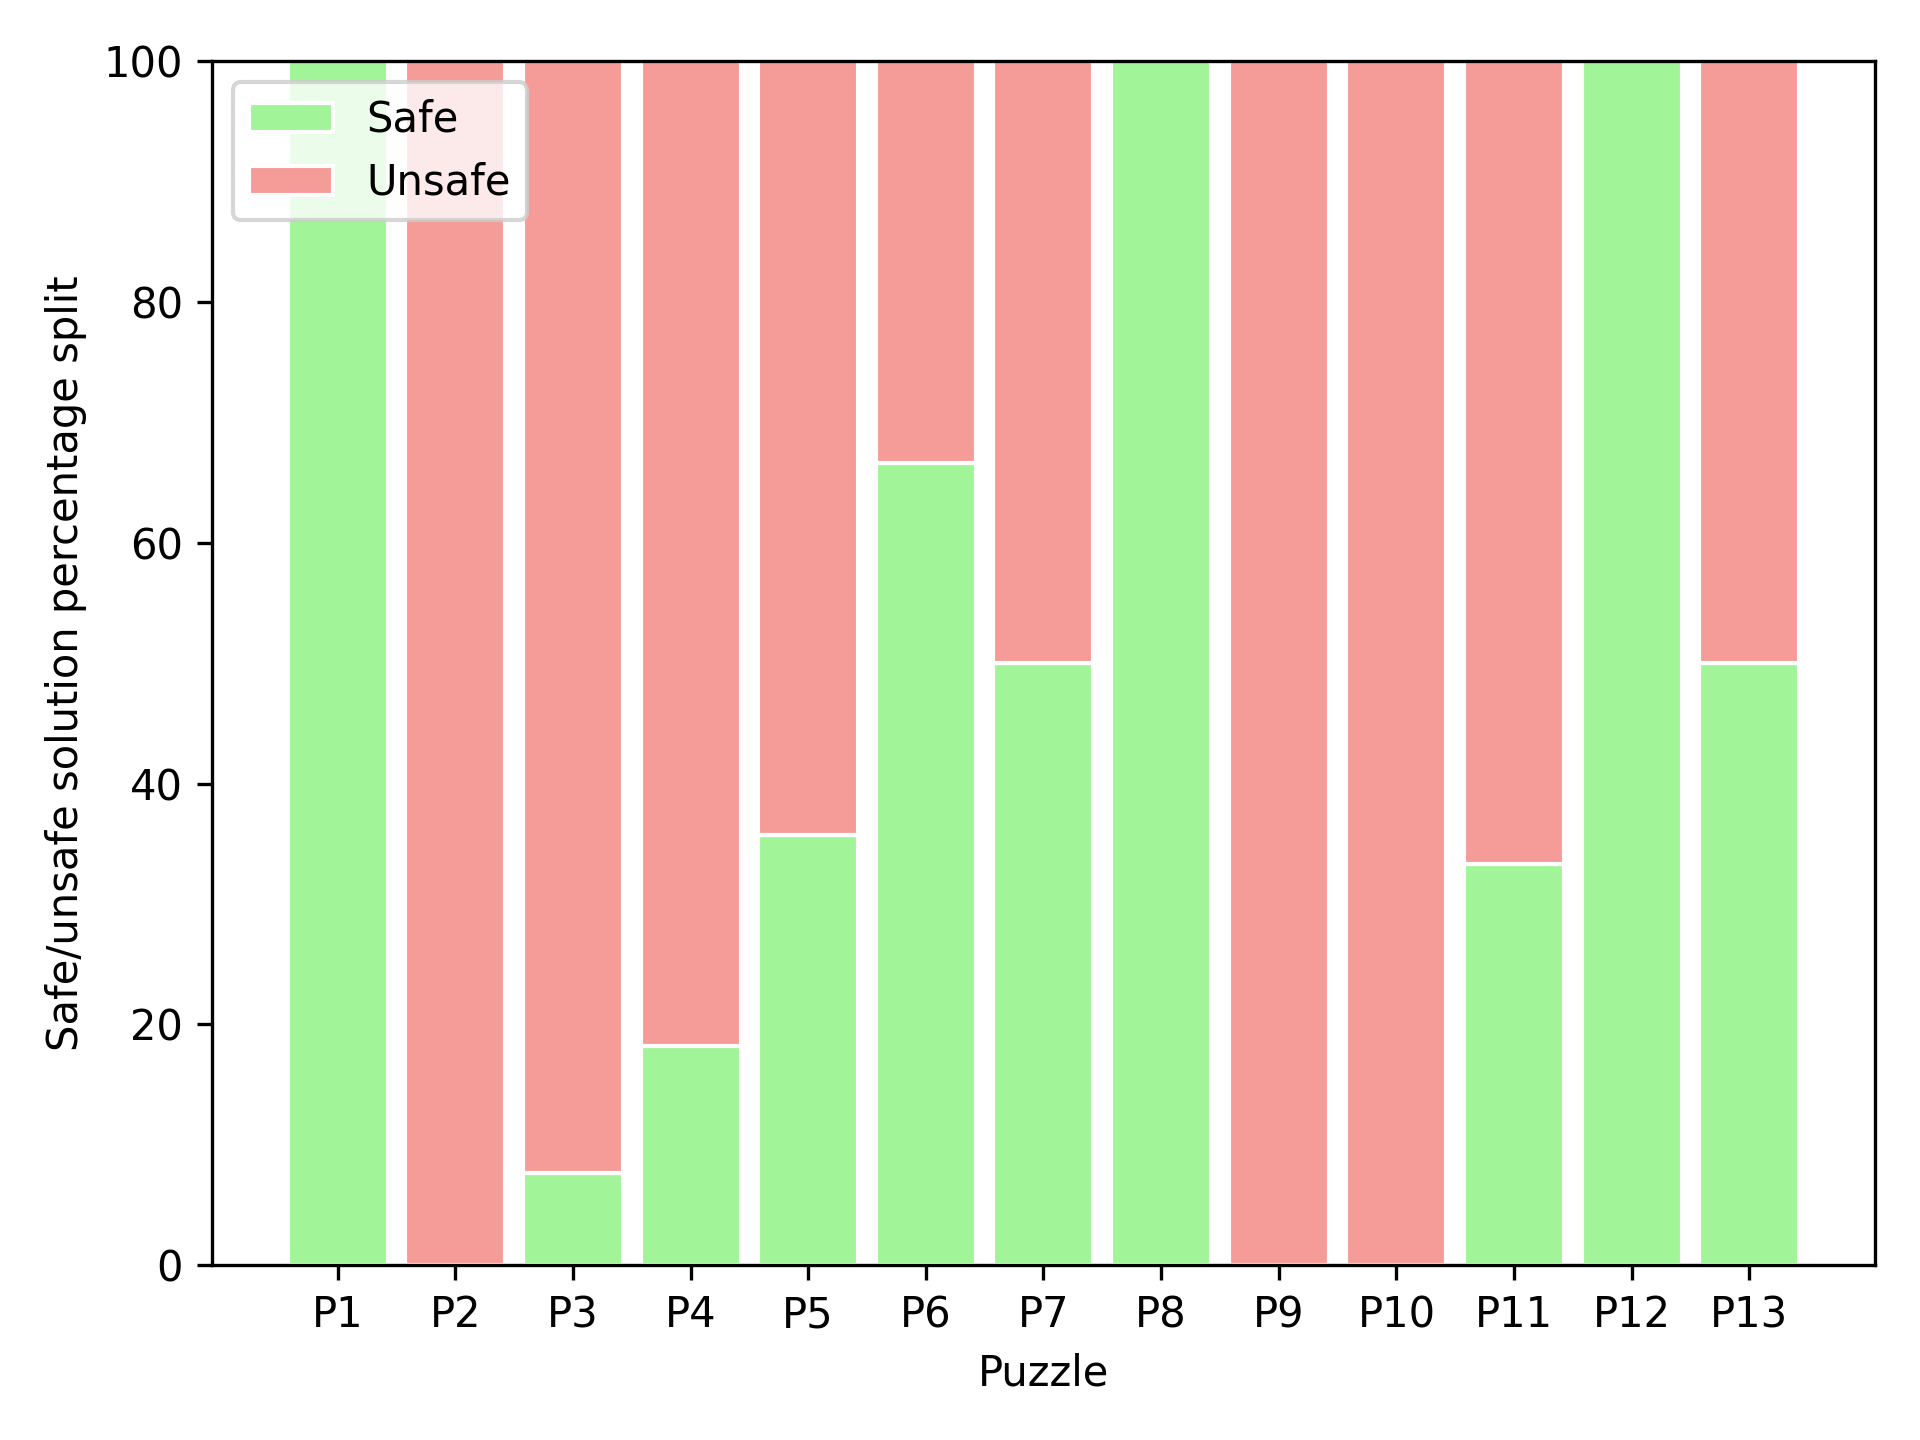
\includegraphics[width=\columnwidth]{img/phase2split.png}
	\caption{Rush Hour planning tasks used in Human-aware Intervention \textbf{with hints}}
	\label{fig:phase2split}
	\end{minipage}
\end{figure}

\subsection{Solution Lengths Compared to the Cost Optimal Solution in the Control and the Condition Groups}
In Section~\ref{sec:costoptimal}, we show evidence from our previous study (Appendix~\ref{apx:rushintervention}) to support the claim that the cost optimal solution to the modified Rush Hour planning task provides a reference solution against which we can compare the user’s solution.
We adopt the same principle to discuss the solutions the human users produced in the Human-aware Rush Hour planning task with hints.
In both cases we use an automated planner to find the cost optimal solutions to the Rush Hour planning tasks.

\begin{table}[tpb]
\begin{tabular}{|l|c|c|c|c|}
\hline
\multirow{2}{*}{PID} & \multicolumn{2}{l|}{Number of Moves} & \multicolumn{2}{l|}{Number of Cars} \\ \cline{2-5} 
    & $P_{observer}$ & $P_{user}$ & $P_{observer}$ & $P_{user}$ \\ \hline
P1  & 24   & 24     & 8    & 8      \\ 
P2  & 30   & 30     & 10   & 10     \\ 
P3  & \textbf{35}   & \textbf{25}     & 10   & 10     \\ 
P4  & 23   & 23     & 9    & 9      \\ 
P5  & \textbf{21}   & \textbf{14}     & 7    & 7      \\ 
P6  & 22   & 22     & 8    & 8      \\ 
P7  & 21   & 21     & 8    & 8      \\ 
P8  & 9    & 9      & 5    & 5      \\ 
P9  & 21   & 21     & 10   & 10     \\
P10 & 24   & 24     & 9    & 9      \\ 
P11 & 26   & 26     & 7	   & 7		\\
P12 & 17   & 17     & 8    & 8		\\
P13 & 21   & 21	    & 8	   & 8		\\	\hline
\end{tabular}
\caption{Optimal costs for the Rush Hour planning tasks $P_{observer}$ and $P_{user}$ optimized for number of moves and number of cars. $P_{observer}$ finds solutions without moving the forbidden vehicle. $P_{user}$ may find a shorter solution while moving the forbidden vehicle.}
\label{tab:optimals}
\end{table}

We use 13 Rush Hour planning tasks in this study.
Table~\ref{tab:optimals} shows the optimal costs for the Rush Hour planning tasks $P_{observer}$ and $P_{user}$, using the optimizing criteria, the \textbf{number of moves} and the \textbf{number of cars}.
Recall that $P_{observer}$ forces the planner to find solutions without using the forbidden vehicle.
In contrast, $P_{user}$ can find shorter solutions while using the forbidden vehicle.
In some cases, $P_{user}$ may produce shorter plans than $P_{observer}$ as evidenced by cost optimal solutions for P3 and P5 when the number of moves is used as the optimizing criterion.

Figure \ref{fig:difficulyphase2} illustrates how the number of moves in human user solutions compare to threshold values derived from the optimal solution produced by a planner.
The charts in the top row are human user solutions to type \textbf{E} puzzles, the middle row are type \textbf{C} puzzles and the bottom row are type \textbf{M} puzzles.
We define the threshold $\alpha$ as the optimal number of moves obtained from the automated planner for $P_{observer}$.
Then we derive a set of threshold values using $\alpha$ as the baseline such that $\lbrace 1.2\times \alpha, 1.4\times \alpha, 1.6\times \alpha, 1.8\times \alpha \rbrace$.
The higher threshold values indicate longer solutions.

In general, the human user solutions are longer than the cost optimal solution produced by a planner for the same planning task.
However, for P8 puzzle, which had the forbidden car in the corner of the board, all but one user found cost optimal solutions.
Human users have difficulty finding solutions closer to the optimal for P2.
The same is observed when the human users solve P2 without hints. 
In our previous study, for puzzles P3 and P5 human users found solutions shorter than the optimal solution for $P_{observer}$.
However, these solutions all require the user to move the forbidden vehicle.
This is not the case when the users solve the planning task with hints.
The reason for this behavior is that we modified the experiment conditions to block the user from moving the forbidden vehicle, which prevented the user from searching for the solution along the same path.

Using Human-aware Intervention with hints, 78\% of the users who attempted the type E puzzles found solutions after the $1.4\times\alpha$ threshold.
For the type C puzzle, 60\% of the users who attempted the puzzle found solutions after the $1.4\times\alpha$ threshold.
For the type M puzzle, this value is 45\%.
This finding indicate that human users take a long time to find solutions to the type E puzzles where the forbidden vehicle is on the edge of the board compared to the type C and type M.
Human users find the solutions faster when the forbidden vehicle is in the middle of the board (type M).

When solving the Rush Hour planning task without hints, 56\% of the users who attempted the type E found solutions after the $1.4\times\alpha$ threshold.
For the type C puzzle, 40\% of the users who attempted the puzzle found solutions after the $1.4\times\alpha$ threshold.
For that experiment we only had one puzzle of the type M.
In that puzzle 90\% of the users found solutions after the $1.4\times\alpha$ threshold.
Similar to the case where they used hints, the time taken to find solutions to the type C puzzles is longer than the type M puzzles.

\begin{figure}[tpb]
  \centering
  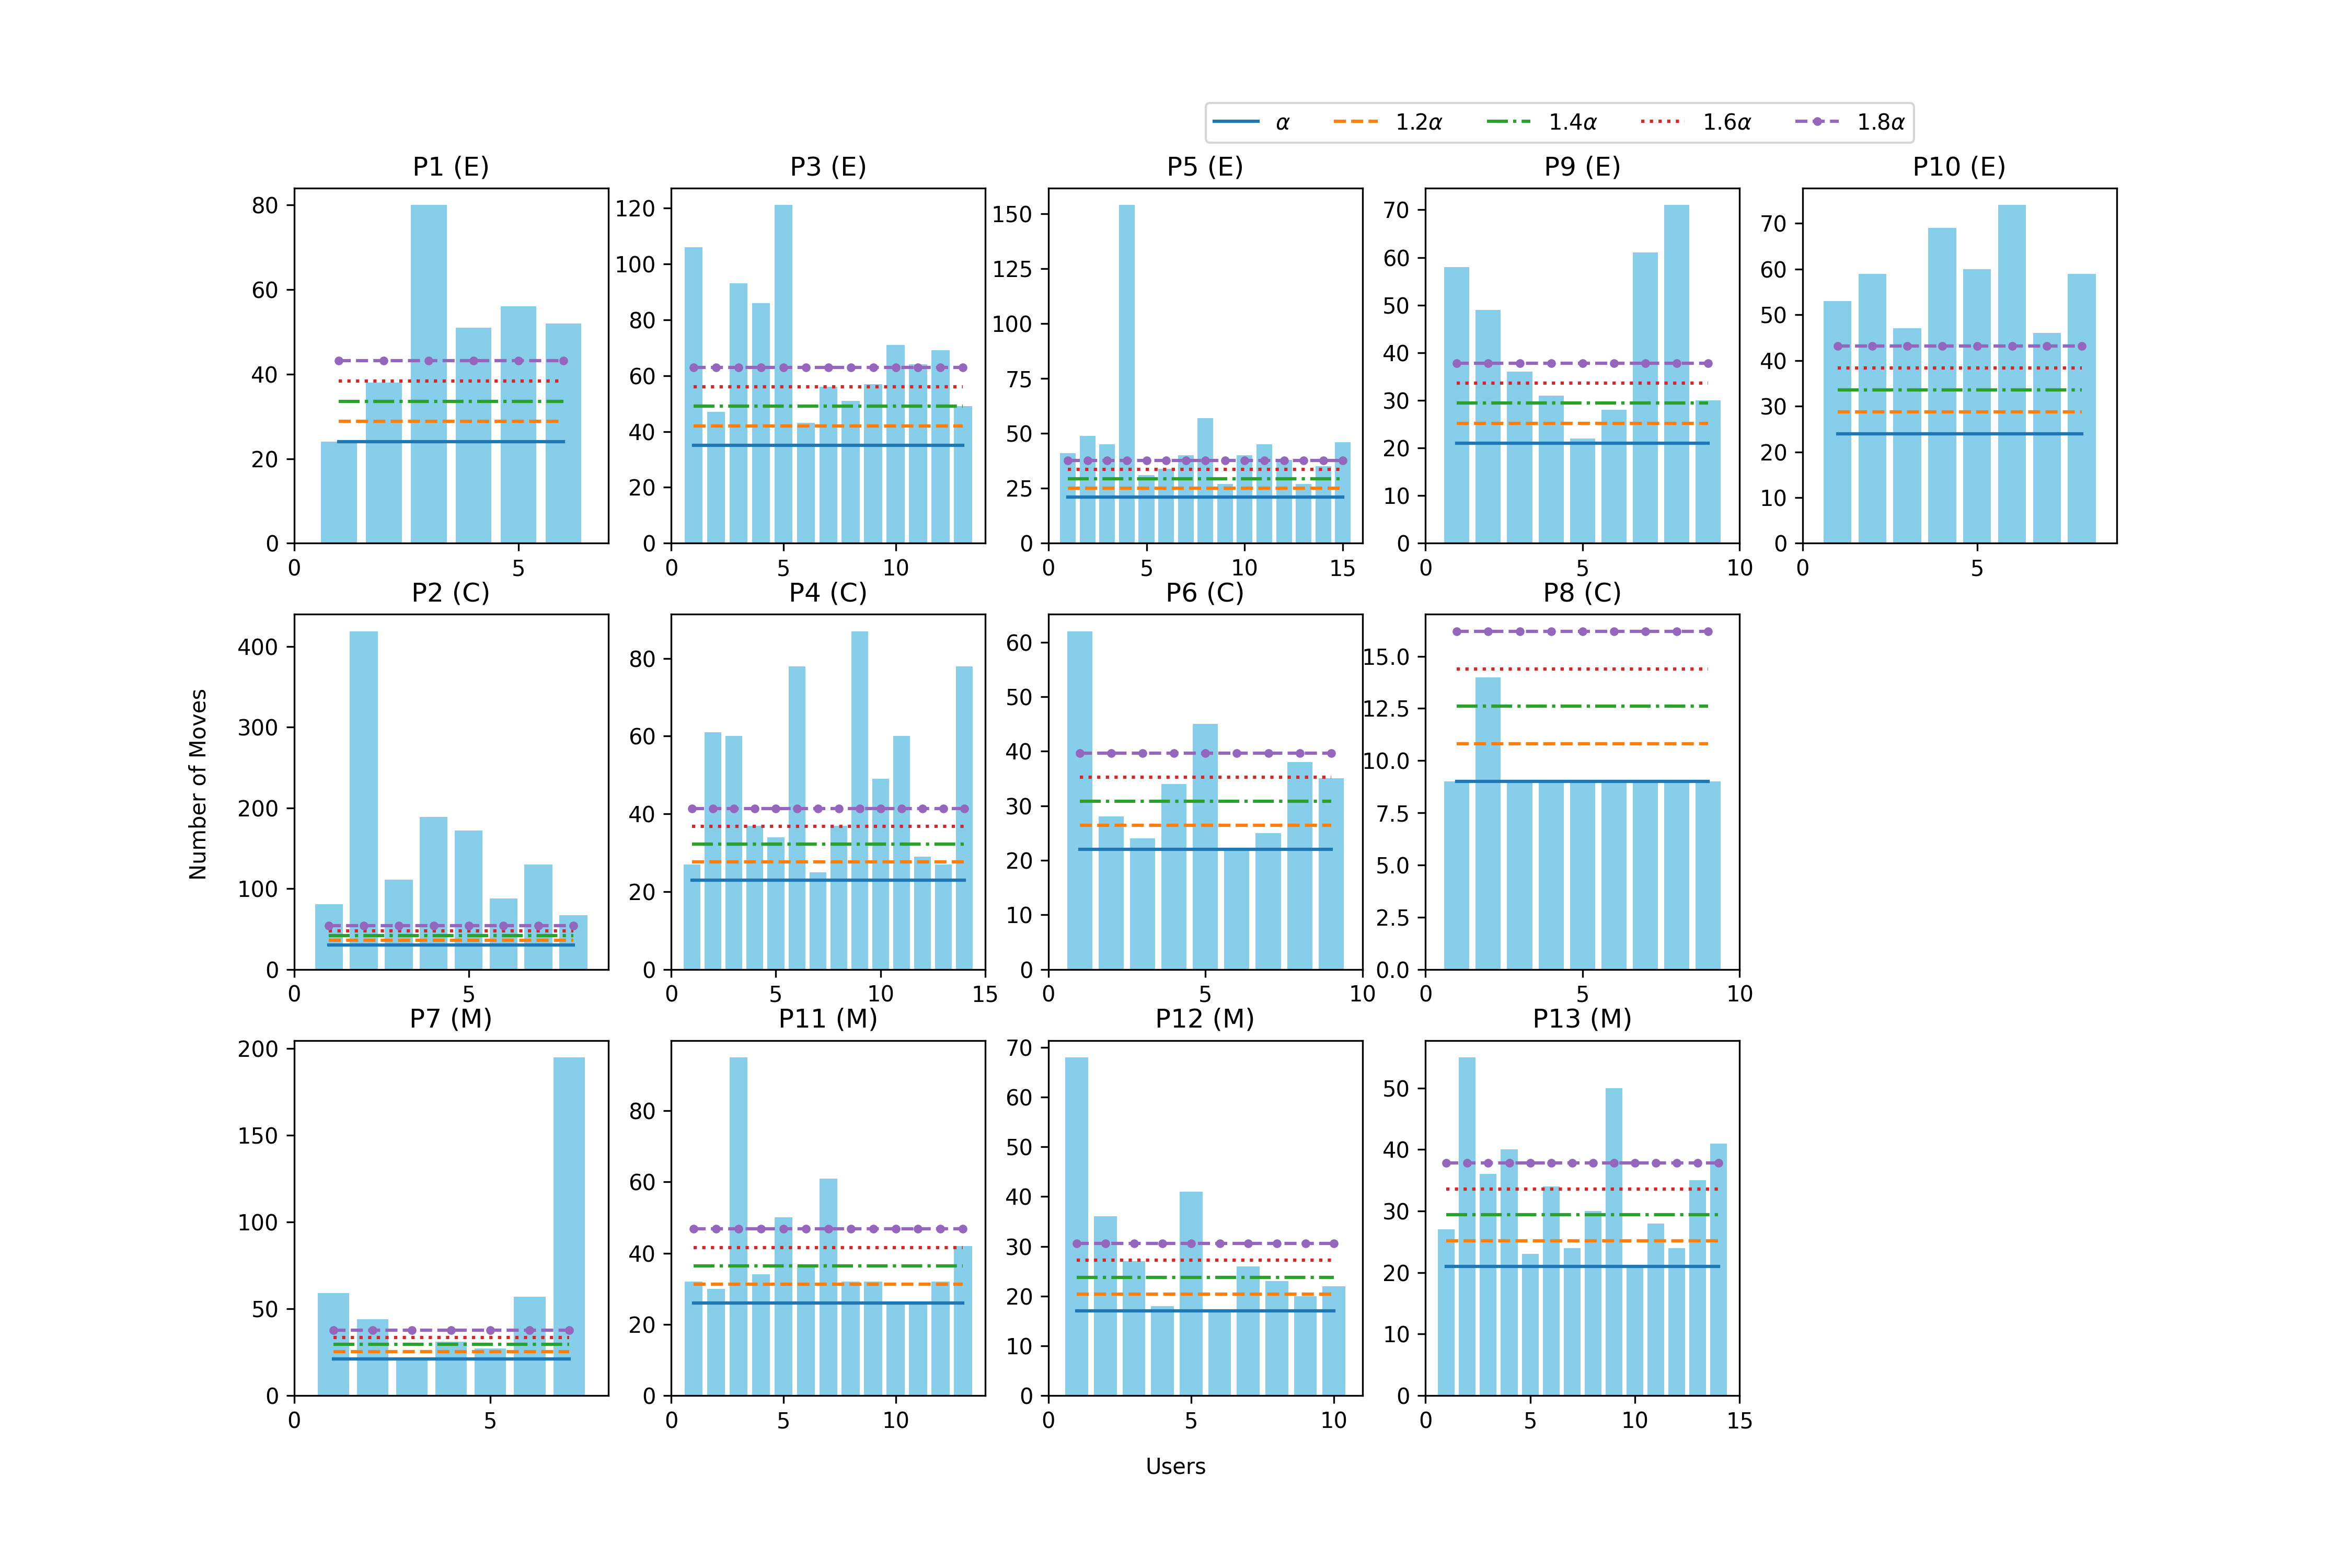
\includegraphics[width=\columnwidth]{img/phase2difficulty.png}
  \caption{Number of moves in the human user solutions compared to the optimal number of moves $\alpha$, and 1.2$\alpha$, 1.4$\alpha$, 1.6$\alpha$, 1.8$\alpha$ number of moves for the puzzles P1 through P13. Within brackets next to the puzzle identifier is the puzzle type per Table~\ref{tab:puzzles}}
  \label{fig:difficulyphase2}
\end{figure}


\subsection{Relationship Between Avoiding the Forbidden Vehicle and the Number of Moves}
\label{sec:relationshipavoidingforbidden}
When the human users solved the Rush Hour planning task without hints, we sorted the solutions by the number of moves in the ascending order and split them into three groups (fast, medium, slow). 
We ensured that the three groups for each puzzle contained approximately equal number of users. 
Table \ref{tab:solvergroupsphase1} summarizes the mean solution length in number of moves for each puzzle and the number of times the forbidden vehicle was moved in fast, medium and slow groups.
There were 46 users in the fast group, 42 in the medium and 48 in the slow group. 

\begin{table}[tpb]
\begin{tabular}{|l|l|l|l|l|l|l|}
\hline
\multicolumn{1}{|c|}{\multirow{2}{*}{PID}} &
  \multicolumn{2}{c|}{Fast} &
  \multicolumn{2}{c|}{Medium} &
  \multicolumn{2}{c|}{Slow} \\ \cline{2-7} 
\multicolumn{1}{|c|}{} &
  \begin{tabular}[c]{@{}c@{}}Mean \\ (St. Dev.)\end{tabular} &
  \begin{tabular}[c]{@{}c@{}}Forbidden\\ Moves\end{tabular} &
  \begin{tabular}[c]{@{}c@{}}Mean \\ (St. Dev.)\end{tabular} &
  \begin{tabular}[c]{@{}c@{}}Forbidden\\ Moves\end{tabular} &
  \begin{tabular}[c]{@{}c@{}}Mean \\ (St. Dev.)\end{tabular} &
  \begin{tabular}[c]{@{}c@{}}Forbidden\\ Moves\end{tabular} \\ \hline
P1  & 25.5 (1.5) & 0  & 41.7 (7.0) & 0  & 64.7 (21.1) & 0  \\ 
P2  & 74.7 (22) & 4  & 137.7 (21) & 16 & 277 (112.5)  & 28 \\ 
P3  & 26.5 (1.9) & 8  & 36.2  (4.3) & 9  & 43.7 (5.6) & 6  \\ 
P4  & 25.2 (1.8) & 1  & 32 (4.1) & 4  & 76  (29.0) & 28 \\ 
P5  & 18.3 (4.0) & 3  & 26  (1.0)  & 2  & 44.75 (24.9) & 13 \\ 
P6  & 22  (0) & 0  & 24.5 (1.3) & 0  & 39.6 (11.0) & 0  \\ 
P7  & 38.5 (7.2) & 5  & 53.3 (8.5) & 16 & 120 (11.7) & 37 \\ 
P8  & 9  (0)  & 0  & 9 (0)  & 0  & 10  (1.1) & 0  \\ 
P9  & 27.8 (3.8) & 8  & 48.6 (10.0) & 12 & 99   (38.7) & 28 \\ 
P10 & 50.3 (7.8) & 11 & 66  (6.9)  & 14 & 127.3 (32.7) & 46 \\ \hline
\end{tabular}
\caption{ The mean number of moves and the frequency of forbidden moves in fast, medium and slow solution groups, when the Rush Hour planning task is \textbf{solved without hints}}
\label{tab:solvergroupsphase1}
\end{table}

We can see that the longer the solutions are the more frequently the users will move the forbidden vehicle. 
Is this relationship statistically significant? 
In order to address this question, we first perform the normality test between the two variables: \textbf{number of moves} and the \textbf{number of times the forbidden car was moved}. 
We used the Shapiro-Wilks test for the two distributions with $H_0:$ the distribution is normally distributed, and $H_A:$ the distribution is not normally distributed. Given $\alpha=0.05$, Shapiro-Wilks test gives that the p-value $<0.05$ for both forbidden vehicle moves and the number of moves. 
Thus we reject $H_0$ for both distributions.

To test the relationship between the number of moves and the forbidden vehicle moves when the hints are not used, we define the null and alternative hypotheses as follows. 
Since we showed that there is evidence that the distributions are not normally distributed, we use the non-parametric test Spearman's Rank Correlation to measure the strength of relationship. 
Let $\rho_s$ be the Spearman's population correlation coefficient:
\begin{itemize}
\item $H_0: \rho_s=0$, there is no correlation between the \textbf{number of moves} and the \textbf{number of times the forbidden car was moved}
\item $H_A: \rho_s\neq0$, there is a correlation between the \textbf{number of moves} and the \textbf{number of times the forbidden car was moved}
\end{itemize}
Given $\alpha=0.05$, Spearman's rank correlation coefficient is $\rho_s=0.52$ and p-value $<0.05$. 
Thus we reject the null hypothesis.

Next, we test whether the correlation between the solution length and the number of forbidden vehicle moves is the same when the human users solve the Rush Hour planning task with hints.
We follow the same procedure as above to split the solutions into fast, medium and slow groups.
Initially, there were 45, 42 and 48 solutions in each group respectively.
However, there were instances where the observer agent did not display any hints during the planning task.
We removed the subjects who did not see any hints for this analysis, leaving 20 users in the fast group, 26 users in the medium group and 35 users in the slow group.
Table~\ref{tab:solvergroupsphase2} shows the mean solution length and the count of forbidden vehicle moves for each puzzle.


To test the relationship between the number of moves and the forbidden vehicle moves when the hints are used, we define the null and alternative hypotheses the same as above.
The test of normality using the Shapiro-Wilks test show that the two variables: number of moves and the number of times the forbidden vehicle was moved, are not normally distributed.
Therefore, we use the Spearman's Rank Correlation test to measure the strength of the relationship between the two variables.
Given $\alpha=0.05$, Spearman's rank correlation coefficient is $\rho_s=0.475$ and p-value $<0.05$. 
Thus, we reject $H_0$.

We conclude that the longer the users spend searching for the solution to the Rush Hour planning task, the more likely they will move the forbidden car. 
This observation is the same for solving the Rush Hour planning problem with and without hints.


\begin{table}[tpb]
\begin{tabular}{|l|l|l|l|l|l|l|}
\hline
\multicolumn{1}{|c|}{\multirow{2}{*}{PID}} &
  \multicolumn{2}{c|}{Fast} &
  \multicolumn{2}{c|}{Medium} &
  \multicolumn{2}{c|}{Slow} \\ \cline{2-7} 
\multicolumn{1}{|c|}{} &
  \begin{tabular}[c]{@{}c@{}}Mean \\ (St. Dev.)\end{tabular} &
  \begin{tabular}[c]{@{}c@{}}Forbidden\\ Moves\end{tabular} &
  \begin{tabular}[c]{@{}c@{}}Mean \\ (St. Dev.)\end{tabular} &
  \begin{tabular}[c]{@{}c@{}}Forbidden\\ Moves\end{tabular} &
  \begin{tabular}[c]{@{}c@{}}Mean \\ (St. Dev.)\end{tabular} &
  \begin{tabular}[c]{@{}c@{}}Forbidden\\ Moves\end{tabular} \\ \hline
P1  & 31 (9.9)   & 0 & 51.5 (0.7)  & 0 & 68 (17)     & 0  \\ %\hline
P2  & 236 (10.7) & 3 & 130         & 1 & 260 (138)   & 10 \\ %\hline
P3  & 47.5 (3.4) & 4 & 61.5 (6.1)  & 5 & 95.4 (19.1) & 6  \\ %\hline
P4  & -          & - & 43.4 (10.9) & 4 & 75.8 (11.3) & 4  \\ %\hline
P5  & 31.7 (3.6) & 1 & 40.8 (2.6)  & 5 & 76.5 (51.9) & 2  \\ %\hline
P6  & -          & - & 34          & 0 & 53.5 (12.0) & 1  \\ %\hline
P7  & 29 (2.8)   & 0 & 50.5 (9.2)  & 3 & 127 (96.2)  & 2  \\ %\hline
P8  & -          & - & -           & - & 14          & 0  \\ %\hline
P9  & 22         & 1 & -           & - & 66 (7.1)    & 5  \\ %\hline
P10 & 49 (3.8)   & 4 & 59 (0)      & 2 & 67.7 (7.1)  & 3  \\ %\hline
P11 & -          & - & -           & - & 68.7 (23.5) & 5  \\ %\hline
P12 & -          & - & -           & - & 41          & 0  \\ %\hline
P13 & 25 (1.7)   & 0 & 31.7 (3.3)  & 2 & 44.4 (7.8)  & 17 \\ \hline
\end{tabular}
\caption{ The mean number of moves and the frequency of forbidden moves in fast, medium and slow solution groups when the Rush Hour planning task is \textbf{solved with hints}. A hyphen (-) indicates that the users who solved that puzzle did not see any hints}
\label{tab:solvergroupsphase2}
\end{table}


\subsection{Usage of Hints in the Condition Group}
In this section we analyze how the users requested hints and discuss the findings to address the question: \textbf{What are the most frequently used hints in different stages of the Rush Hour planning task?}

From the 91 subjects who requested hints during the puzzle solving task 49 users (54\%) requested less than 2 hints. 20 subjects requested between 3--5 hints (22\%). 
There are 4 subjects each in 6--8 hint and 9--11 hint request categories. 
14 subjects requested more than 11 hints (15\%).
In Table~\ref{tab:speedsandrequests}, we report the total number of requests for each hint  made by users in the slow, medium and fast groups.
``Undo'' refers to the instances where the user actually moved the forbidden vehicle and saw the alert message in Figure~\ref{fig:badcar}.
The ``Undo'' alert is seen by users in all three groups.
In all three groups ``Show the next best move'' is the most requested hint. 
This finding corroborates the subjective helpfulness rating the users gave for the hints in the post-study survey where the hint ``Show the next best move'' was rated as the most helpful compared to the others.
The second most requested option in all three groups is the ``Ignore'', where the users disregard the Human-aware intervention.
The least used hint in the slow group is ``Show the vehicles that must be moved''.
The same can be observed in the fast group.
In the medium group, the least requested hint is ``Restart''.
Intuitively, the users in the fast group did not request for the ``Restart'' hint.
This is because we count the number of moves before and after the restart as the solution length and restarting the puzzle might push the user out of the fast group.
Figure~\ref{fig:speedrequest} illustrates the request frequency distribution with the error bars.


\begin{table}[tpb]
\begin{tabular}{|l|cccccc|}
\hline
\multirow{2}{*}{Speed} & \multicolumn{6}{c|}{Hint} \\ \cline{2-7} 
 & \multicolumn{1}{c|}{Undo} & \multicolumn{1}{c|}{Remaining} & \multicolumn{1}{c|}{Must Move} & \multicolumn{1}{c|}{Next Best} & \multicolumn{1}{c|}{Restart} & Ignore \\ \hline
Slow & 57 & 36 & 10 & 131 & 14 & 73 \\ \hline
Medium & 23 & 9 & 17 & 120 & 5 & 42 \\ \hline
Fast & 18 & 11 & 3 & 90 & 0 & 32 \\ \hline
\end{tabular}
\caption{Number of times each hint was selected by users in the slow, medium and fast solution groups}
\label{tab:speedsandrequests}
\end{table}

\begin{figure}[tpb]
  \centering
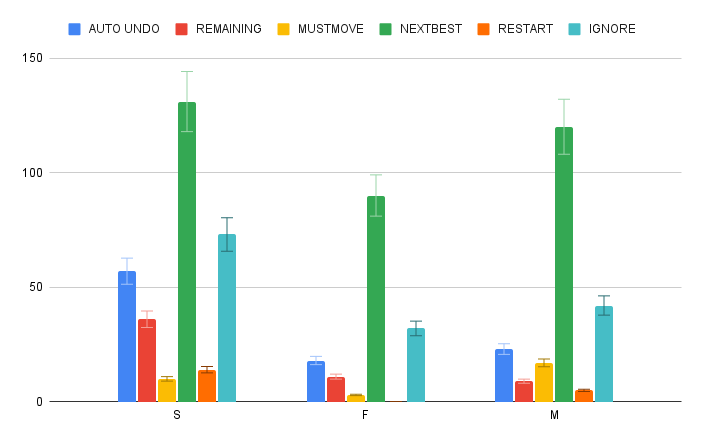
\includegraphics[width=0.8\columnwidth]{img/speedreq.png}
  \caption{Number of requests for each hint type in slow (S), medium (M) and fast (F) solution groups.}
  \label{fig:speedrequest}
\end{figure}

We now analyze the hint request patterns considering the three Rush Hour planning task types E, M, C.
In Table~\ref{tab:groupsandrequests}, we report the total number of requests for each hint requested for the three planning task types.
For each planning task types, the most requested hint is ``Show the next best move''.
The same was observed when considering user's solution speed.
The second most requested option is ``Ignore''.
The least requested hint is ``Restart'' for type C and M planning tasks.
For type E, the least requested hint is ``Show the vehicles that must be moved''.
The ``Undo'' option was triggered for all three planning tasks.
Figure~\ref{fig:groupandrequest} illustrates the request frequency distribution with the error bars.
\begin{table}[tpb]
\begin{tabular}{|l|cccccc|}
\hline
\multirow{2}{*}{Type} & \multicolumn{6}{c|}{Selected Hint} \\ \cline{2-7} 
 & \multicolumn{1}{c|}{Undo} & \multicolumn{1}{c|}{Remaining} & \multicolumn{1}{c|}{Must Move} & \multicolumn{1}{c|}{Next Best} & \multicolumn{1}{c|}{Restart} & Ignore \\ \hline
E & 40 & 18 & 6 & 145 & 12 & 66 \\ \hline
M & 31 & 13 & 6 & 100 & 2 & 38 \\ \hline
C & 27 & 25 & 18 & 96 & 5 & 43 \\ \hline
\end{tabular}
\caption{Number of times each hint was selected by users in the Rush Hour planning task types E, M, C}
\label{tab:groupsandrequests}
\end{table}

\begin{figure}[tpb]
  \centering
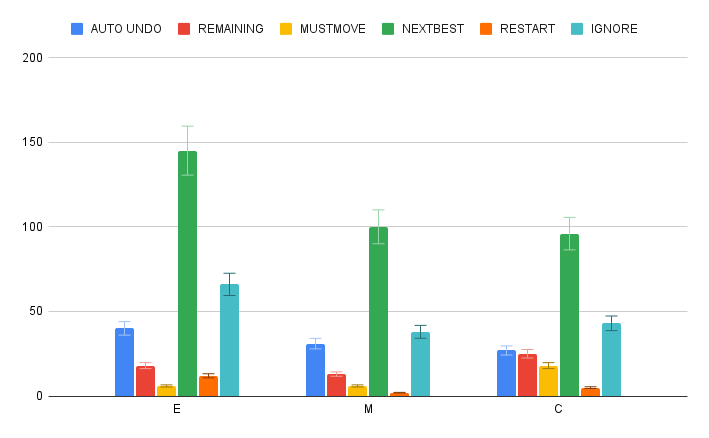
\includegraphics[width=0.8\columnwidth]{img/typeandreq.png}
  \caption{Number of requests for each hint in the Rush Hour planning task types E, M, C with error bars.}
  \label{fig:groupandrequest}
\end{figure}

\begin{table}[tpb]
\resizebox{\columnwidth}{!}{% 
\begin{tabular}{|l|llllllllllllllllllll|}
\hline
Request Number & \multicolumn{1}{l|}{1} & \multicolumn{1}{l|}{2} & \multicolumn{1}{l|}{3} & \multicolumn{1}{l|}{4} & \multicolumn{1}{l|}{5} & \multicolumn{1}{l|}{6} & \multicolumn{1}{l|}{7} & \multicolumn{1}{l|}{8} & \multicolumn{1}{l|}{9} & \multicolumn{1}{l|}{10} & \multicolumn{1}{l|}{11} & \multicolumn{1}{l|}{12} & \multicolumn{1}{l|}{13} & \multicolumn{1}{l|}{14} & \multicolumn{1}{l|}{15} & \multicolumn{1}{l|}{16} & \multicolumn{1}{l|}{17} & \multicolumn{1}{l|}{18} & \multicolumn{1}{l|}{19} & 20 \\ \hline
Undo & 57 & 10 & 6 & 6 & 3 & 4 & 2 & 2 & 2 & 1 & 1 & 1 & 0 & 1 & 0 & 0 & 0 & 0 & 0 & 0 \\ \cline{1-1}
Remaining & 6 & 5 & 10 & 6 & 3 & 4 & 1 & 0 & 1 & 1 & 1 & 3 & 2 & 1 & 1 & 1 & 1 & 1 & 0 & 1 \\ \cline{1-1}
Next Best & 14 & 35 & 27 & 22 & 20 & 18 & 15 & 17 & 16 & 17 & 14 & 12 & 12 & 10 & 9 & 8 & 8 & 8 & 8 & 7 \\ \cline{1-1}
Must Move & 4 & 5 & 4 & 3 & 3 & 2 & 1 & 1 & 0 & 0 & 2 & 0 & 1 & 1 & 1 & 1 & 1 & 0 & 0 & 0 \\ \cline{1-1}
Ignore & 8 & 19 & 23 & 19 & 13 & 10 & 11 & 5 & 4 & 2 & 2 & 3 & 2 & 3 & 3 & 3 & 1 & 1 & 2 & 1 \\ \cline{1-1}
Restart & 2 & 6 & 2 & 4 & 5 & 0 & 0 & 0 & 0 & 0 & 0 & 0 & 0 & 0 & 0 & 0 & 0 & 0 & 0 & 0 \\ 
\hline
Total & 91 & 80 & 72 & 60 & 47 & 38 & 30 & 25 & 23 & 21 & 20 & 19 & 17 & 16 & 14 & 13 & 11 & 10 & 10 & 9 \\ \hline
\end{tabular}%
}
\caption{The total number of hints requested from each type sorted by the request number - part 1}
\label{tab:reqnumberbreakdown1}
\end{table}


\begin{table}[tpb]
\resizebox{\columnwidth}{!}{% 
\begin{tabular}{|l|rrrrrrrrrrrrrrrrrr|}
\hline
Request Number & \multicolumn{1}{l|}{21} & \multicolumn{1}{l|}{22} & \multicolumn{1}{l|}{23} & \multicolumn{1}{l|}{24} & \multicolumn{1}{l|}{25} & \multicolumn{1}{l|}{26} & \multicolumn{1}{l|}{27} & \multicolumn{1}{l|}{28} & \multicolumn{1}{l|}{29} & \multicolumn{1}{l|}{30} & \multicolumn{1}{l|}{31} & \multicolumn{1}{l|}{32} & \multicolumn{1}{l|}{33} & \multicolumn{1}{l|}{34} & \multicolumn{1}{l|}{35} & \multicolumn{1}{l|}{36} & \multicolumn{1}{l|}{37} & 38 \\ \hline
Undo & 0 & 0 & 0 & 0 & 0 & 0 & 0 & 0 & 0 & 0 & 0 & 0 & 0 & 0 & 0 & 0 & 0 & 0 \\ \cline{1-1}
Remaining & 0 & 1 & 0 & 0 & 1 & 0 & 1 & 1 & 1 & 0 & 1 & 1 & 0 & 1 & 1 & 1 & 0 & 0 \\ \cline{1-1}
Next Best & 6 & 6 & 6 & 4 & 4 & 4 & 4 & 3 & 3 & 1 & 1 & 1 & 1 & 0 & 0 & 0 & 0 & 0 \\ \cline{1-1}
Must Move & 0 & 0 & 0 & 0 & 0 & 0 & 0 & 0 & 0 & 0 & 0 & 0 & 0 & 0 & 0 & 0 & 0 & 0 \\ \cline{1-1}
Ignore & 2 & 0 & 1 & 3 & 1 & 1 & 0 & 0 & 0 & 2 & 1 & 0 & 1 & 0 & 0 & 0 & 1 & 1 \\ \cline{1-1}
Restart & \multicolumn{1}{l}{0} & \multicolumn{1}{l}{0} & \multicolumn{1}{l}{0} & \multicolumn{1}{l}{0} & \multicolumn{1}{l}{0} & \multicolumn{1}{l}{0} & \multicolumn{1}{l}{0} & \multicolumn{1}{l}{0} & \multicolumn{1}{l}{0} & \multicolumn{1}{l}{0} & \multicolumn{1}{l}{0} & \multicolumn{1}{l}{0} & \multicolumn{1}{l}{0} & \multicolumn{1}{l}{0} & \multicolumn{1}{l}{0} & \multicolumn{1}{l}{0} & \multicolumn{1}{l}{0} & \multicolumn{1}{l|}{0} \\ \hline
Total & 8 & 7 & 7 & 7 & 6 & 5 & 5 & 4 & 4 & 3 & 3 & 2 & 2 & 1 & 1 & 1 & 1 & 1 \\ \hline
\end{tabular}%
}
\caption{The total number of hints requested from each type sorted by the request number - part 2}
\label{tab:reqnumberbreakdown2}
\end{table}


\begin{figure}[tpb]
  \centering
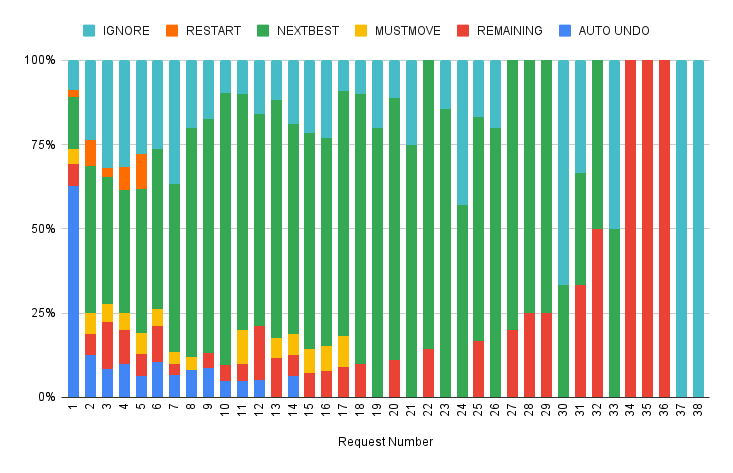
\includegraphics[width=0.9\columnwidth]{img/reqdistribution.png}
  \caption{Percentage split for hints for each request number}
  \label{fig:reqdistribution}
\end{figure}

Figure~\ref{fig:reqdistribution} illustrates the percentage split between the hints the subjects selected each time the Human-aware Intervention agent recognized that the user needed help.
The x-axis, Request Number refers to the sequence of requests in the ascending order. 
For example, Request Number 1 means the first choice the subjects made when the Human-aware Intervention agent recognized that the user needed intervention, Request Number 2 is the second choice the subjects made and so on.
The maximum number of hints requested by a user is 38.
Tables~\ref{tab:reqnumberbreakdown1} and ~\ref{tab:reqnumberbreakdown2} show the counts of  each hint requested.
The first hint seen by majority of the users (63\%) is the alert message indicating the forbidden vehicle is moved.
One reason for this observation is that we set a threshold for the number of steps for the Human-aware Intervention agent to start displaying the hints.
For each planning task, we use lower value of the number of moves in the cost optimal solution to $P_{user}$ or $P_{observer}$ as the threshold (see Table~\ref{tab:optimals}).
For all planning tasks except P3 and P5 the number of moves in the cost optimal solutions to $P_{user}$ or $P_{observer}$ are the same.
In P3 and P5 the solution to $P_{user}$ is shorter than the solution to $P_{observer}$.
The threshold is required to ensure that the logistic regression classifier we use to recognize intervention has enough data to be used as input in the beginning.
This means that the Human-aware Intervention agent does not perform any recognition  from the start of the planning task until the threshold is exceeded.
From the 57 subjects who saw the forbidden vehicle move alert message as the first hint, only 5 subjects (1 user who solved P2, 2 users who solved P4, 1 user who solved P5 and 1 user who solved P7) saw it after they had gone past the corresponding thresholds.
The remaining 52 subjects missed the interaction with the Human-aware Intervention agent due to the constraint in the machine learning method we use in this study.
The other reason could be that the subjects had difficulty recognizing the forbidden vehicle on their own although they were primed to think about its presence. 
The Table~\ref{tab:firsthint} in Appendix~\ref{apx:hintsstudy} summarizes the raw data for the solutions produced by the 57 subjects.

Figure~\ref{fig:reqdistribution} further corroborates the finding that the hint ``Show next best move'' is the most requested hint.
Moreover, it is chosen by the subjects early as well as during the late stages of their planning tasks.
The hint ``Show the remaining number of moves'' is requested less often at first and more often towards the end.
The hint ``Show the vehicles that must be moved'' is only requested early.
The hint ``Ignore'' is chosen during all stages of the planning task.
The reason for this observation is because we leave it to the subject's discretion to decide when they want to turn off the Interactive Human-aware Intervention agent.
The hint ``Restart'' is used only in early requests.
It is also the least requested hint.

To examine how the hints are requested for each planning task, we consider the first ten hint requests and the mean remaining number of steps in the planning task at each request.
The mean remaining number of steps for a hint $\mathcal{N}$ for the $i^{th}$ request  $i= \lbrace 1, \ldots, 10\rbrace$ during a planning task  is computed as follows:
\begin{equation}
\frac{\sum (\textup{number of steps in solution}) - (\textup{number of steps before request } \mathcal{N})}{\textup{number of users requesting } \mathcal{N}}
\end{equation}
The mean remaining number of steps indicates how early in the planning task a particular hint is requested.
We limit the analysis to the first ten hint requests because that threshold covers the majority of the subjects who used hints.
Recall that only 14 subjects requested more than 11 hints.
We breakdown the findings by planning task type: C, E and M.

Figure~\ref{fig:requesttypec} illustrates how users request hints in type C planning tasks.
Table~\ref{tab:requesttypec} in the Appendix~\ref{apx:hintsstudy} contains the data used to generate the graphs in Figure~\ref{fig:requesttypec}.
We have seen in Figure~\ref{fig:difficulyphase2}, that the users who solved the planning task P2 took a long time to find the solution.
In contrast, users who solved the P8 planning task found solutions quicker and closer to the number of moves in the cost optimal solution.
The subjects attempting the P2 planning task have moved the forbidden vehicle multiple times (``Undo'' hint in many requests).
They have also requested the ``Show the next best move'' hint in all ten requests because they were having difficulty finding solution for the puzzle.
The ``Ignore'' option is chosen only in the first six requests.
The ``Restart'' option is chosen only once.
The hint ``Show the remaining number of moves'' is chosen only once, very early in the planning task (mean remaining moves 387). 
The maximum number of moves to solve P2 is 419.
In contrast, the subjects attempting the P8 planning task only requested hints 4 times.
In this case they only requested the ``Show the next best move'' hint early on with 4 and 3 remaining number of steps on average.
Later they turned off the hints when they were 2 and 1 move away from the solution on average.
The subjects who attempted the P4 and P6 planning tasks saw the ``Undo'' hint early.
They also requested the ``Show the next best move'' hint throughout the puzzle solving task.
The subjects attempting the P4 and P6 planning tasks used the hint ``Show the vehicles that must be moved'' more often compared to the subjects who attempted P2 and P8.
The subjects attempting the P4 planning task used the hints ``Show the remaining number of moves'' more often than subjects attempting P2, P6 and P8.
For the planning task P4, the subjects requested restarts when there the mean number of moves remaining is between 50 and 60. 
\begin{figure}[tpb]
  \centering
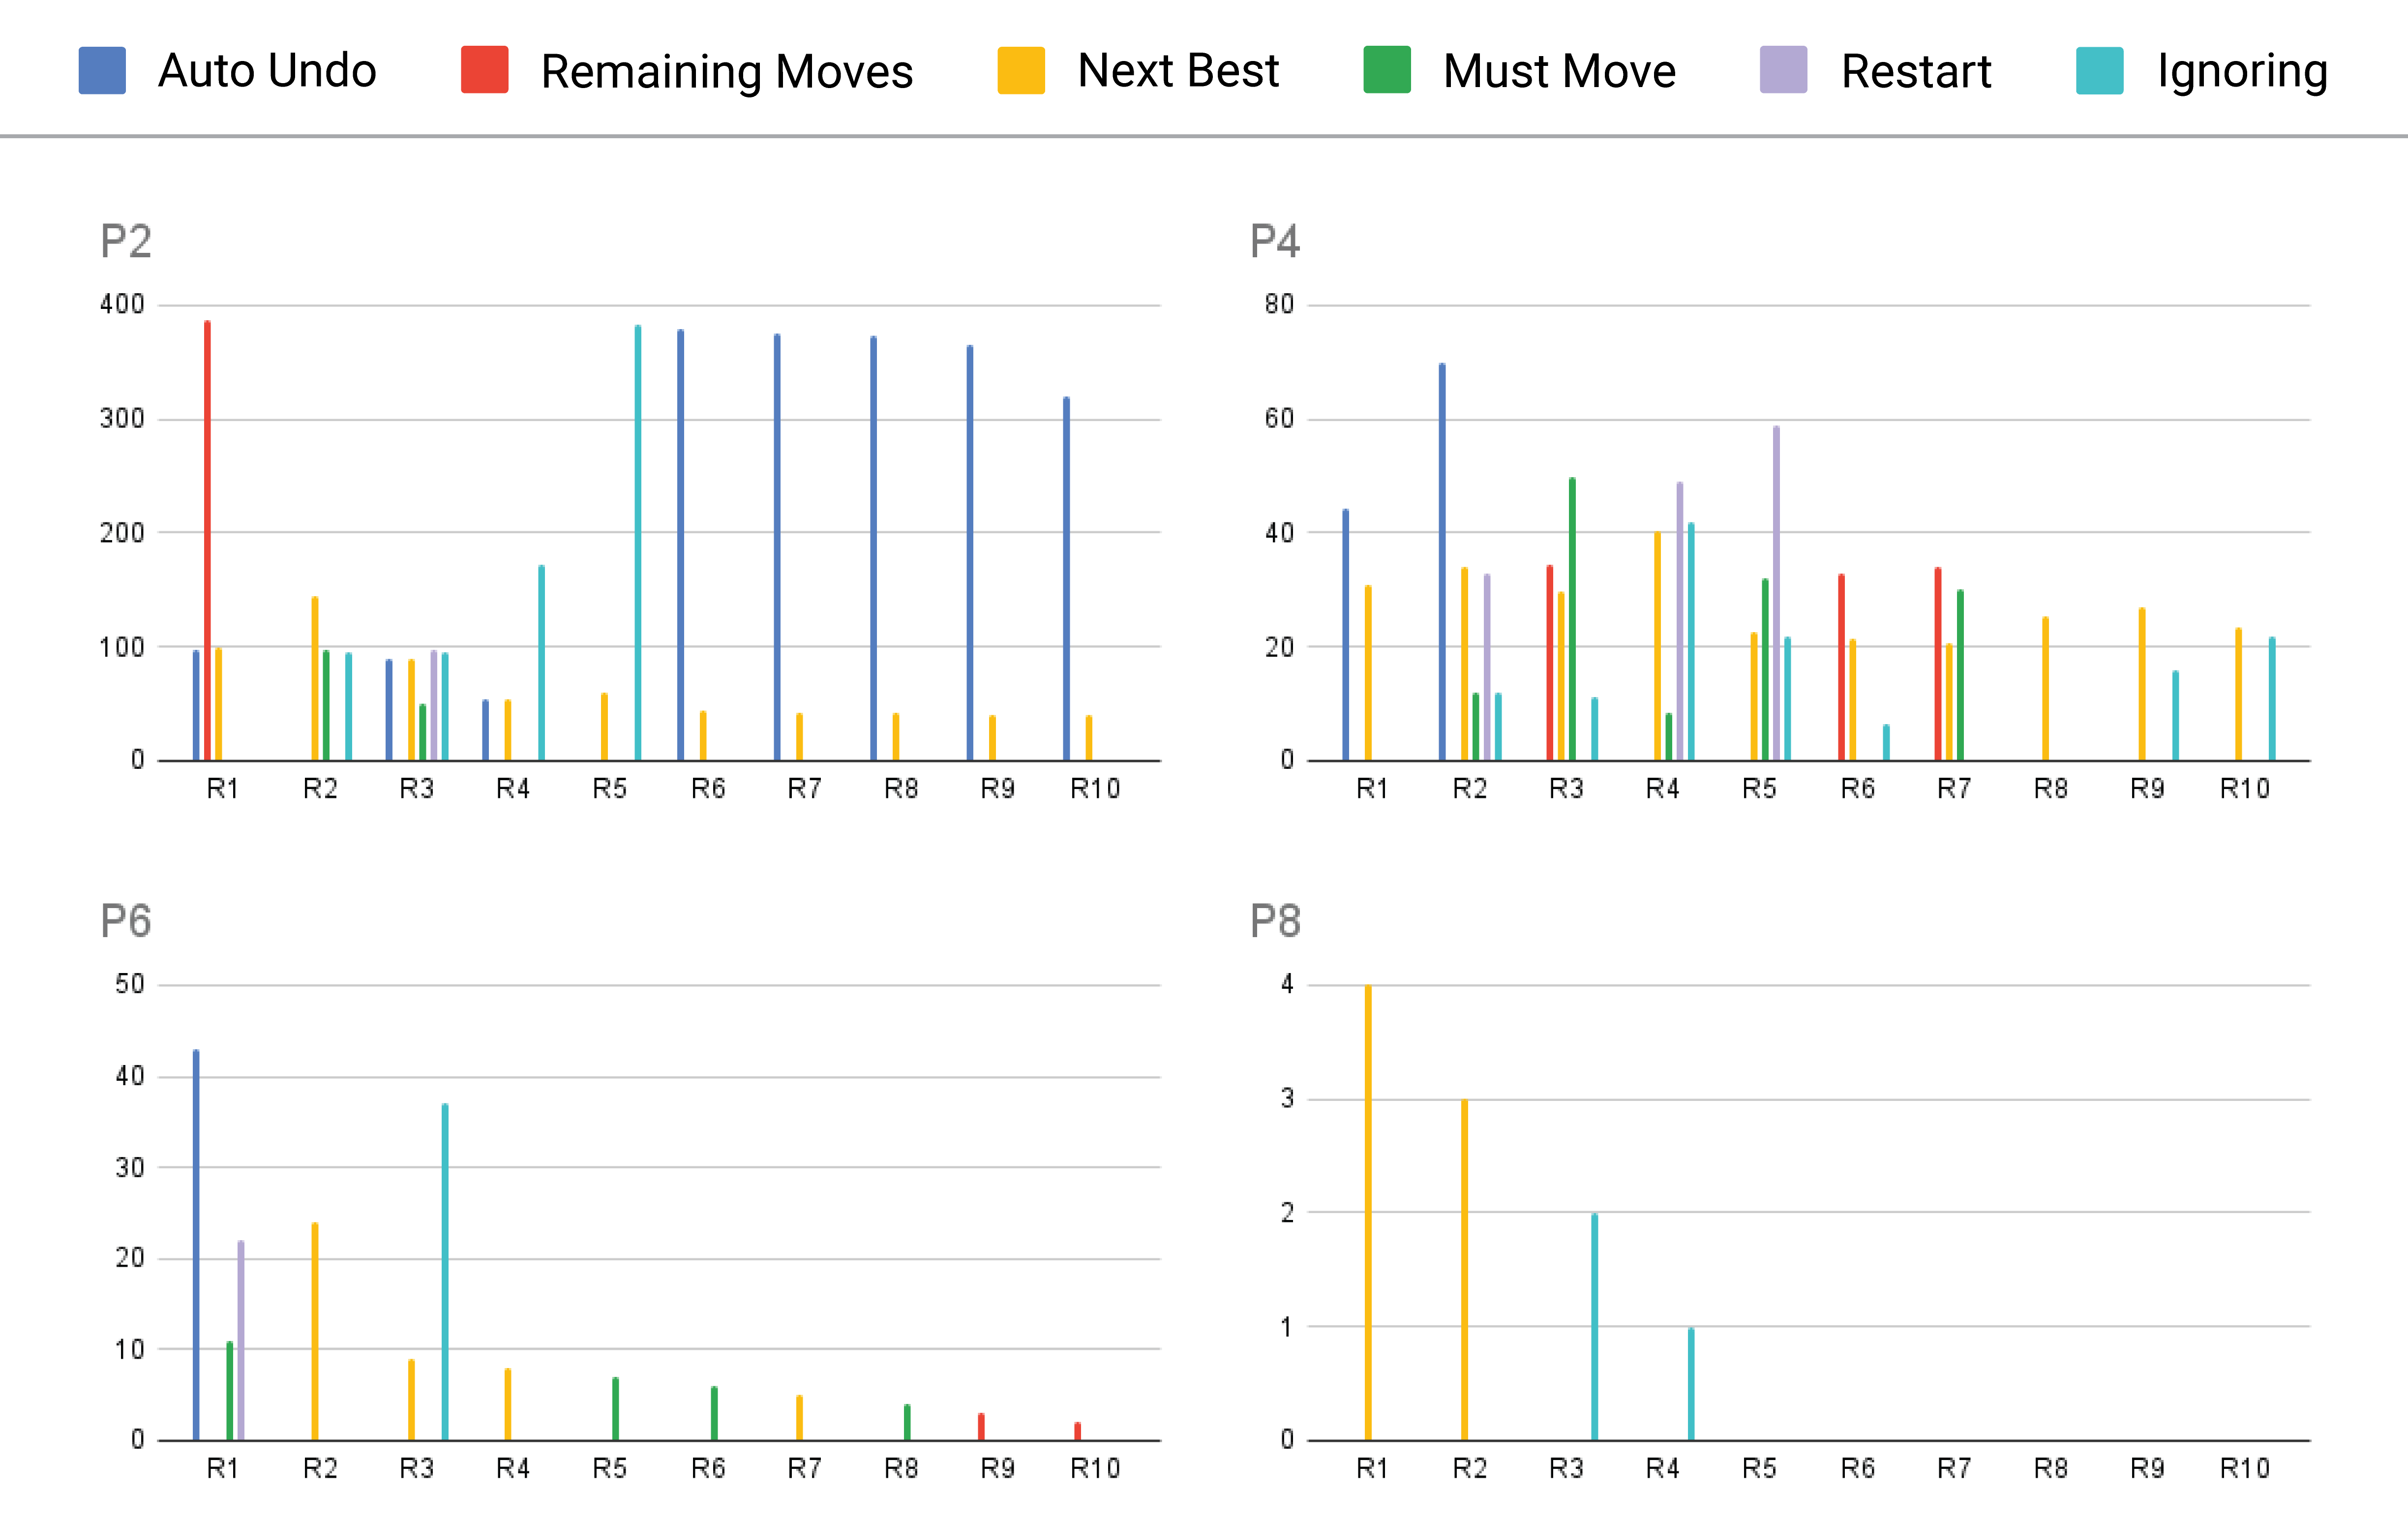
\includegraphics[width=\columnwidth]{img/requesttypec.png}
  \caption{Hint request distribution for type C planning tasks}
  \label{fig:requesttypec}
\end{figure}


Figure~\ref{fig:requesttypee} illustrates how users request hints in type C planning tasks.
Table~\ref{tab:requesttypee} in the Appendix~\ref{apx:hintsstudy} contains the data used to generate the graphs in Figure~\ref{fig:requesttypee}.
Similar to the hint distribution in type C planning tasks, subjects attempting type E tasks also request the hint ``Show the next best move'' in the first ten requests.
The hint ``Show the remaining number of moves'' is requested between the first and the fifth request.
However, for planning tasks P3 and P5, this hint request appears more often.
The hint ``Restart'' is also requested between the first and the fifth request.
For the P3 and P5 planning tasks the ``Ignore'' hint is requested throughout the first ten requests.
The subjects attempting type E planning tasks also moved the forbidden vehicle multiple times early on.
\begin{figure}[tpb]
  \centering
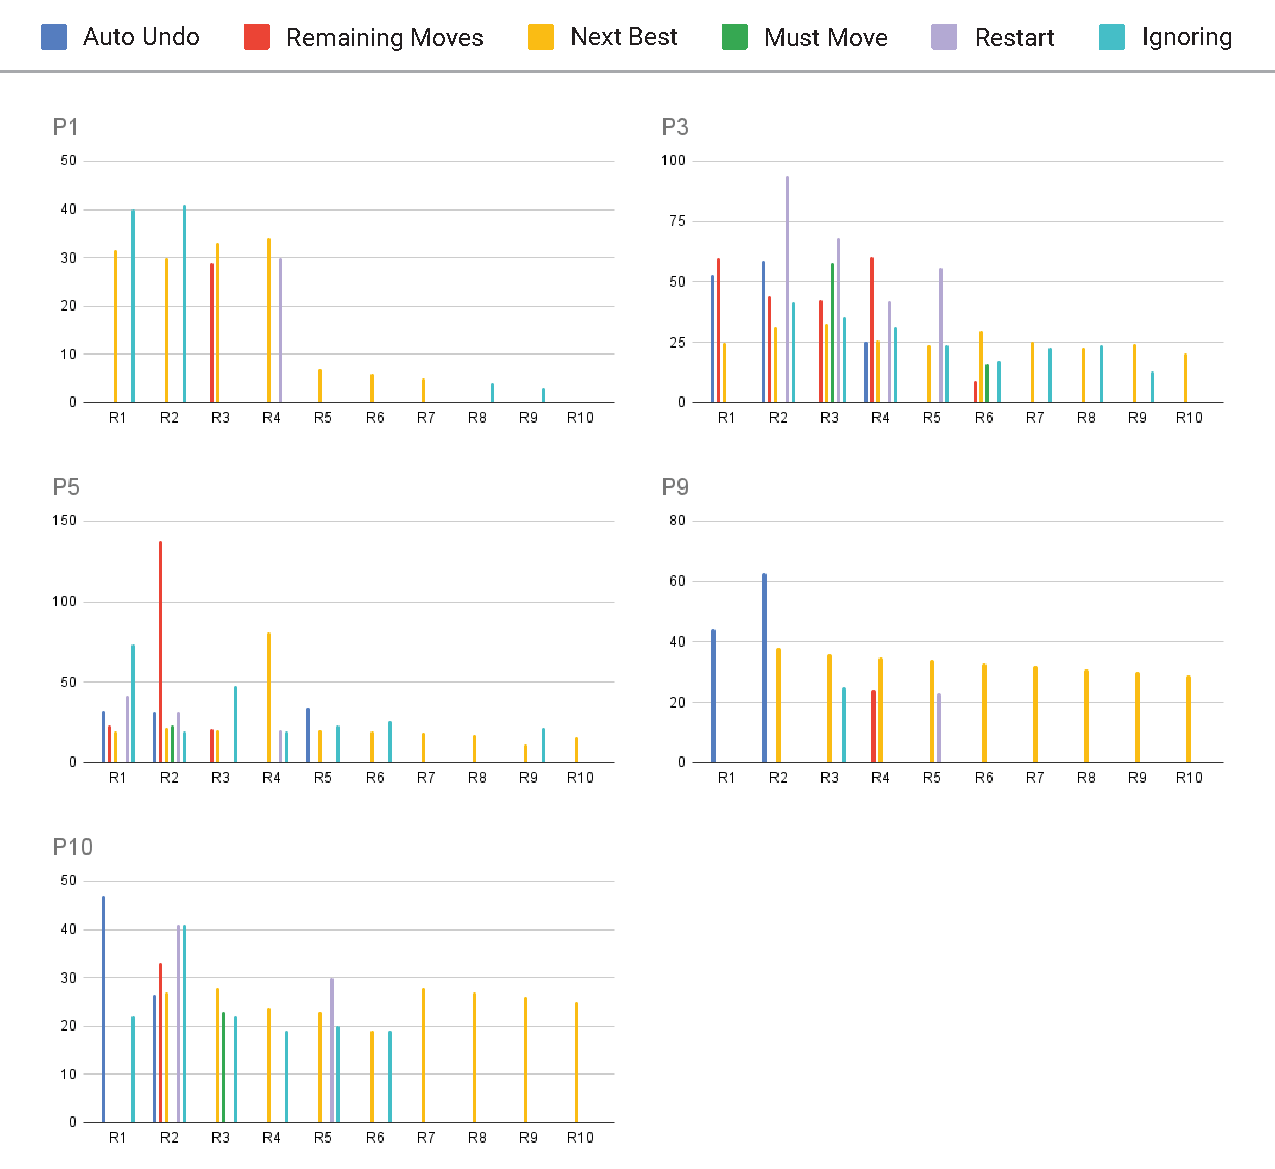
\includegraphics[width=\columnwidth]{img/set-3d.pdf}
  \caption{Hint request distribution for type E planning tasks}
  \label{fig:requesttypee}
\end{figure}

Figure~\ref{fig:requesttypem} illustrates how users request hints in type M planning tasks.
Table~\ref{tab:requesttypem} in the Appendix~\ref{apx:hintsstudy} contains the data used to generate the graphs in Figure~\ref{fig:requesttypem}.
Similar to type C and E, the hint ``Show the next best move'' is requested often in type M planning tasks.
For the planning task P7, the hint ``Show the remaining number of moves is requested more often compared to the other planning tasks in type M.
The ``Restart'' hint is not a common choice among subjects who attempted type M puzzles.
Only users attempting P13 planning task requested a restart.
The users attempting P13 planning task also moved the forbidden vehicle multiple times.
For the planning task P12, we only have one subject using the hints.
The subject requested the hint ``Show the vehicles that must be moved'' early in the planning task.
Then the user requested the ``Show the next best move'' hint 3 times and closer toward the end of the task opted to turn off the hints.

\begin{figure}[tpb]
  \centering
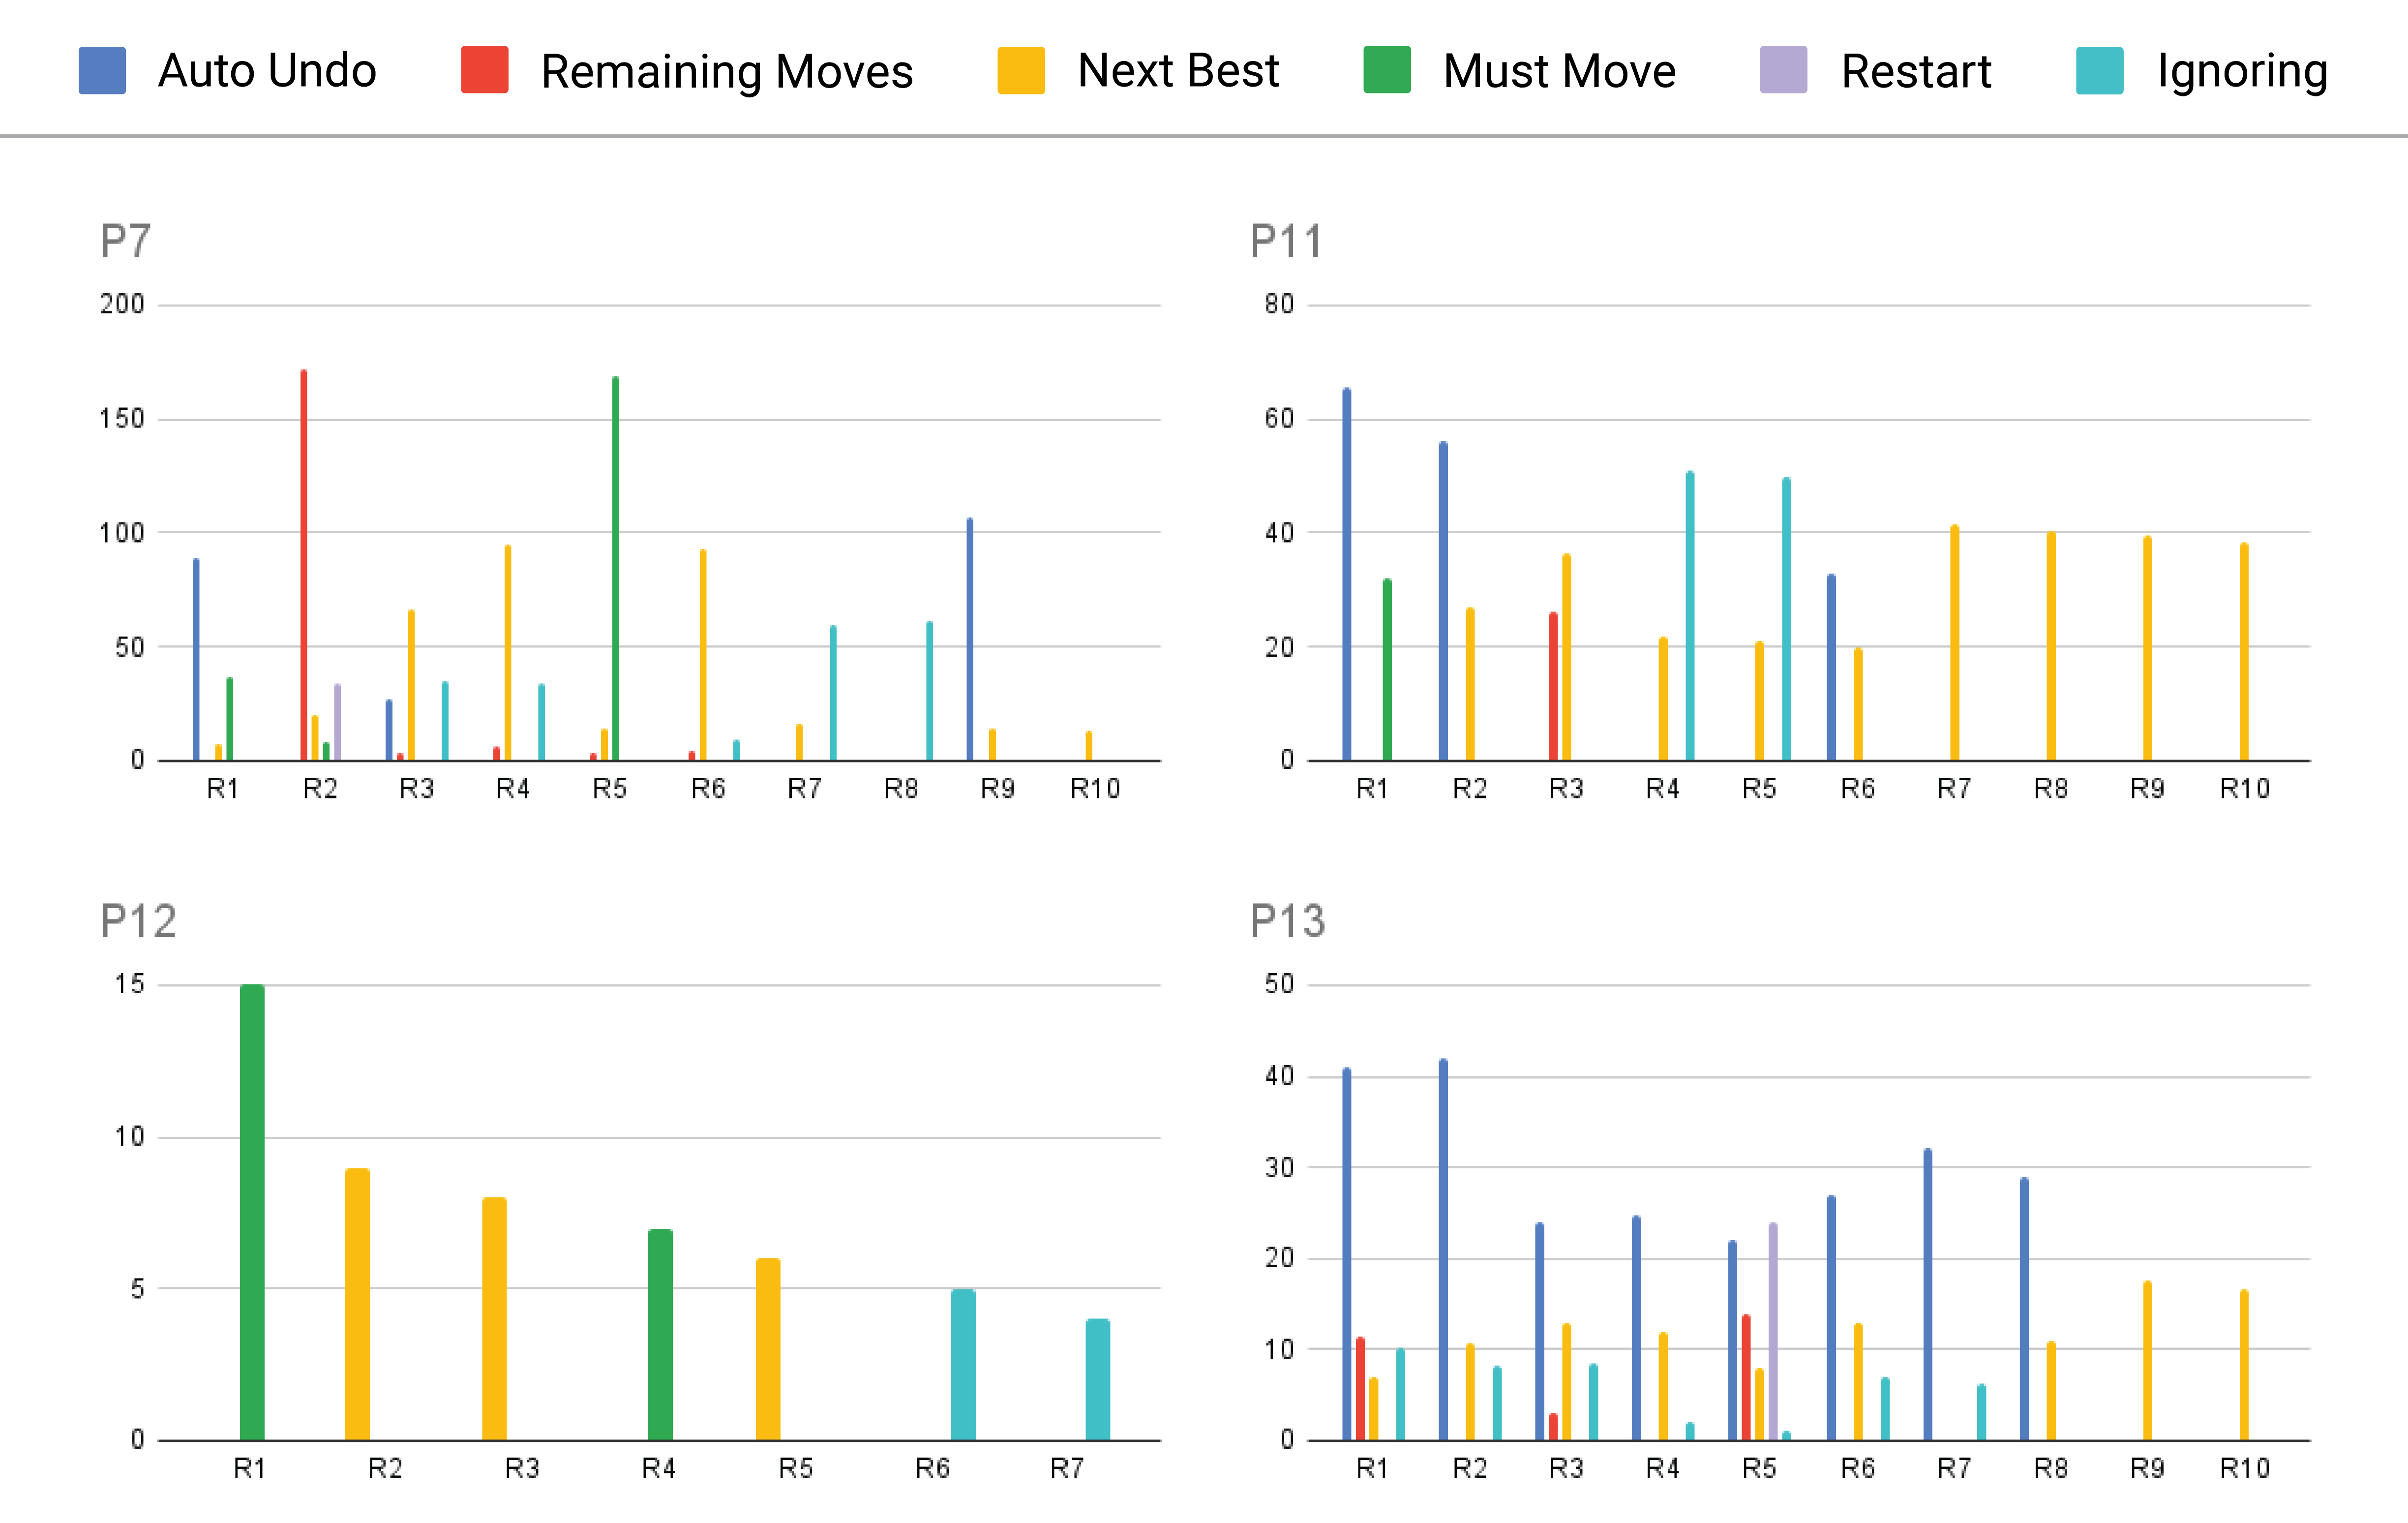
\includegraphics[width=\columnwidth]{img/requesttypem.png}
  \caption{Hint request distribution for type M planning tasks}
  \label{fig:requesttypem}
\end{figure}

\subsection{The Effectiveness of the Interactive Human-aware Intervention}
In Section~\ref{sec:relationshipavoidingforbidden}, we conclude that in order help the user avoid the forbidden vehicle, the Interactive Human-aware Intervention agent must direct the user toward the cost optimal solution for the planning task.
In this section, we evaluate how successful the interactive Human-aware Intervention model has been in moving the user's solution closer to the cost optimal solution using the hints.
Recall that the hints are properties derived from the cost optimal solution and the fact landmarks of $P_{observer}$.
We want to address the following questions:
\begin{enumerate}
\item Does the Interactive Human-aware Intervention have an effect on the solution length?
\item Does the Interactive Human-aware Intervention help move the user closer to the optimal solution?
\item Does seeing a help video move the user closer to the optimal solution?
\end{enumerate}

We introduce the following evaluation metrics.
\begin{enumerate}
\item The number of moves in the human user's solution
\item The difference from the cost optimal solution (defined later)
\item The latest time a fact landmark is eventually achieved 
\item The number of times a fact landmark is lost and regained
\end{enumerate}
The question 1 is answered using the evaluation metric 1.
The question 2 is answered using the evaluation metrics 2, 3 and 4.
The question 3 is answered using the evaluation metrics 2, 3 and 4.
We use the data from the control and condition groups for the planning tasks P1, P2, P4, P6, P7, P8, P9 and P10 for the evaluation.
We remove the planning tasks P3 and P5 because for those two tasks, the cost optimal solution while moving the forbidden vehicle is shorter than the cost optimal solution without moving the forbidden vehicle.
We also remove the planning tasks P11, P12 and P13 because these tasks are only used in the condition group.

\subsubsection{Using the Landmarks}
\label{sec:usingthelandmarks}
To derive the landmark based evaluation metrics, we examine how landmarks are achieved in cost optimal solutions generated by an automated planner for a given Rush Hour planning task.
We use the algorithm advanced by Hoffmann et al. \citeyear{hoffman2004lm} to generate the \textit{Greedy Necessary Fact Landmarks} for the planning task $P_{observer}$ and the actions that have the landmarks as post-conditions.
The algorithm uses a data structure called the Landmark Generation Graph (LGG) to find the landmarks and the greedy necessary orders between them. 
Nodes in LGG are the fact landmarks and the edges are the greedy necessary orders. 
Starting from the goal (the first landmark candidates), the algorithm uses the back-chaining process to find the earliest actions that can be used to achieve each landmark. 
Here, early means a greedy approximation of reachability from the initial state. 
The landmark achievers are actions grounded with the objects that must be moved to solve the planning task from the current state.

In order to analyze how the landmarks are achieved in the solution, we use the Fast Downward planner configured with the admissible heuristic Landmark-cut (\texttt{lmcut}) to generate 100 cost optimal plans for each planning task.
Figure~\ref{fig:achievement} illustrates how landmarks are achieved in five cost optimal plans for the planning tasks P1, P2, P4, P6, P7, P8, P9 and P10.
\begin{figure}[tpb]
  \centering
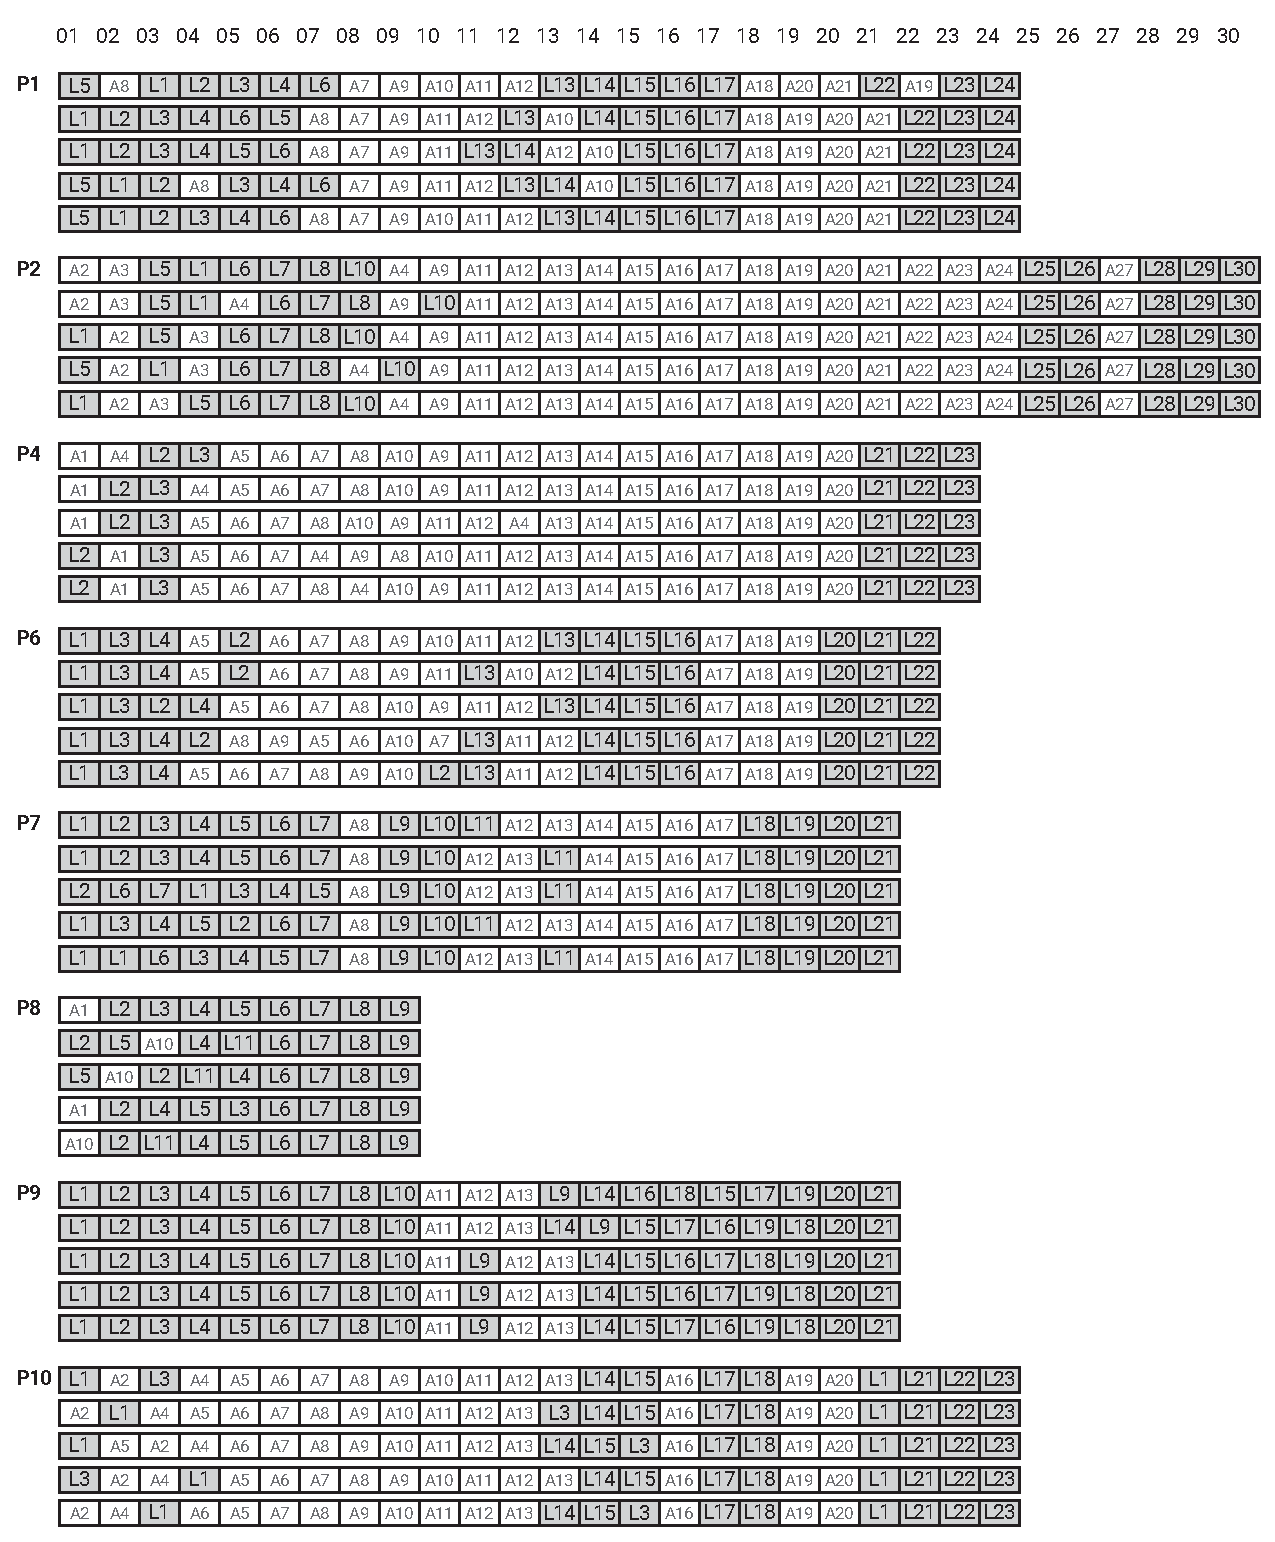
\includegraphics[width=\columnwidth]{img/landmarks.pdf}
  \caption{Landmark achieving patterns in five cost optimal solutions generated by the automated planner. The figures are scaled to reflect the solution length. Actions that achieve the landmarks are in gray cells. Other actions are in white cells. Note that the landmark identifiers L1, L2, $\ldots$ are unique to the planning task.}
  \label{fig:achievement}
\end{figure}
We manually examine the 100 cost optimal plans for each planning task identify frequently occurring landmark achievement patterns.
We see that in all cost optimal solutions the landmarks are achieved in \textit{clusters}.
We use the notation $[ Lj, \ldots ]$ to represent a \textbf{landmark cluster}, where $Lj, j\in\mathbb{N}$ refers to the landmark identifier.
Actions that are not landmarks that appear in the cost optimal plan are denoted with the identifier $(Ak, \ldots), k\in\mathbb{N}$.
Actions that the users execute, but do not appear in the cost optimal plans are denoted with the identifier $(Ul, \ldots), l\in\mathbb{N}$.
The landmark and action identifiers are unique to the planning task.
We denote this as $\langle Pi\rangle [Lj, \ldots] (Ak, \ldots) $, where $Pi$ refers to the planning task identifier, $i=\lbrace 1, 2, 4, 6, 7, 8, 9, 10\rbrace$.

There are groups of actions that achieve some landmarks early in the solution.
For example, consider the cost optimal solutions for the planning task P1 in Figure~\ref{fig:achievement}.
The cost optimal solution for P1 has 24 moves.
The cluster $[L1, L2, L3, L4, L5, L6]$ in the planning task P1 appear very early in the cost optimal solution.
The cluster $[L22, L23, L24]$ appear at the end most of the time.
The cluster $[L15, L16, L17]$ appear together in the middle after $L14$ has been achieved.
The cluster $[L13, L14]$ appear together in the middle before  the cluster $[L15, L16, L17]$.
The condensed representation applied to the cost optimal plans for the planning tasks P1, P2, P4, P6, P7, P8, P9, P10 are as follows:
\begin{itemize}
\item $\langle P1\rangle [L1, L2, L3, L4, L5, L6] (A8) (A7,A9) (A12) [L13, L14] (A10)$ \\ $[L15, L16, L17] (A18, A19, A20, A21) [L22, L23, L24]$
\item  $\langle P2\rangle [L1, L5, L6, L7, L8, L10] (A2, A3, A4, A9)$ \\ $(A11, A12, A13, A14, A15, A16, A17, A18, A19, A20, A21, A22, A23, A24)$ \\ $[L25 L26](A27)[L28, L29, L30]$
\item  $\langle P4\rangle [L2, L3](A1, A4, A5, A6, A7, A8, A9, A10, A11, A12, A13, A14, A15, A16, A17, A18, A19, A20)$\\$[L21, L22, L23]$
\item  $\langle P6\rangle [L1, L2,L3,L4](A5, A6, A7, A8, A9, A10)$ \\ $(A11,A12) [L13][L14, L15, L16](A17,A18,A19)[L20, L21, L22]$
\item  $\langle P7\rangle [L1, L2,L3,L4,L5,L6,L7,L9,L10](A8)[L11]$ \\ $(A12, A13, A14, A15, A16, A17)[L18,L19,L20,L21]$
\item  $\langle P8\rangle (A1,A10) [L2,L3,L4,L5,L6,L7,L8,L9,L10]$
\item  $\langle P9\rangle [L1,L2,L3,L4,L5,L6,L7,L8,L9,L10](A11, A12, A13)$\\$[L14,L15,L16,L17,L18,L19,L20,L21]$
\item  $\langle P10\rangle [L1,L3] (A2,A4,A5) (A6,A7,A8,A9,A10,A11,A12,A13) [L13,L14,L15](A16)$ \\ $[L17,L18] (A19,A20) [L1,L21,L22,L23]$
\end{itemize}

\begin{figure}[tpb]
\centering
	\begin{minipage}[b]{0.46\columnwidth}
	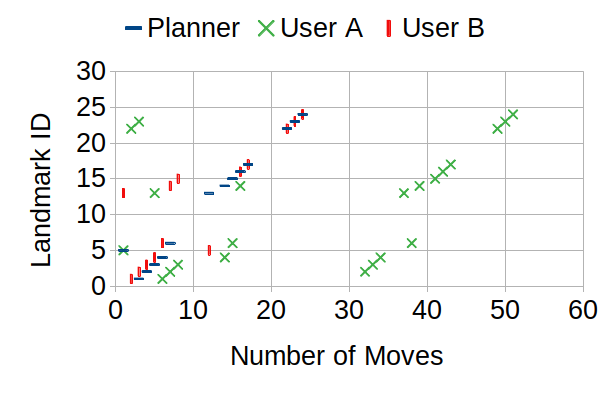
\includegraphics[width=\columnwidth]{img/landmarkp1.png}
	\caption{Human users achieving landmarks for the planning task P1}			
	\label{fig:p1}
	\end{minipage}
	\quad
	\begin{minipage}[b]{0.50\columnwidth}
	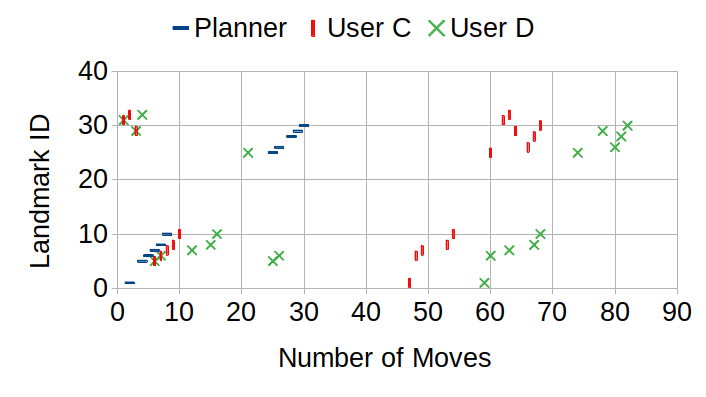
\includegraphics[width=\columnwidth]{img/landmarkp2.png}
	\caption{Human users achieving landmarks for the planning task P2}
	\label{fig:p2}
	\end{minipage}
\end{figure}

Although we can extract common patterns in achieving landmarks when the planning task is solved by an automated planner, this is not the case when human users solve planning tasks.
Figure~\ref{fig:p1} illustrates how two human subjects: A and B achieve the landmarks for the planning task P1 compared to an automated planner.
User B has achieved the landmarks for P1 similar to the automated planner.
There are also a few instances where the same landmark was lost and regained later (i.e. same y-value for different x-values).
Because user B achieved the landmarks similar to the automated planner, the user has been able to solve the planning task in fewer number of moves compared to the user A.
In contrast, user A has taken more number of moves to achieve the landmarks.
Consequently, user A's solution is longer.
Both user A and B has eventually achieved the landmark clusters similar to the automated planner.
Figure~\ref{fig:p2} illustrates how human subjects C and D achieve the landmarks for the planning task P2.
Here too, we can see how the landmark clusters are distributed within the solution produced by the automated planner.
We can see that user C has achieved the early landmark cluster similar to the automated planner.
However, some actions the user executed have caused him/her to lose those landmarks and having to regain them later around the $50^{th}$ move.
User D has lost the early landmark cluster twice before eventually regaining them around the $60^{th}$ move.
User C's solution is shorter compared to user D.
Therefore, when evaluating the human user solutions we monitor only the planning task's landmarks for when they are achieved for the last time and also how often they are regained.

We modify the condensed plan representation discussed above to include the two landmark evaluation metrics: (1) the latest time a fact landmark is eventually achieved and (2) the number of times a fact landmark is lost and regained.
We remove the actions that are not landmarks that appear in the cost optimal plan, i.e., $(Ak, \ldots), k\in\mathbb{N}$ as well as the actions that the users execute, but do not appear in the cost optimal plans, i.e., $(Ul, \ldots), l\in\mathbb{N}$.
The landmark cluster notation is modified as $[Lj(n), \ldots]$, where $Lj, j\in\mathbb{N}$ refers to the landmark identifier and $n\in\mathbb{N}$ corresponds to the evaluation metric value.
For example, if we use the new condensed plan representation for user A's solution to denote the latest time the landmarks are achieved, it will be as follows:
\begin{multline}
\langle P1\rangle [L1(6), L2(32), L3(33), L4(34), L5(1), L6(38)] [L13(37), L14(39)] \\ [L15(41), L16(42), L17(43)] [L22(49), L23(50), L24(51)]
\end{multline}
Using the new condensed plan representation for user A's solution to denote the number of times the landmarks are lost and regained:
\begin{multline}
\langle P1\rangle [L1(1), L2(2), L3(2), L4(2), L5(1), L6(2)] [L13(2), L14(2)] \\ [L15(1), L16(1), L17(1)] [L22(2), L23(2), L24(1)]
\end{multline}
The latest times when the landmarks are achieved by the human subjects attempting the planning tasks P1, P2, P4, P6, P7, P8, P9 and P10 with the Interactive Human-aware Intervention are shown in Tables~\ref{tab:p1landmarkachievement}, ~\ref{tab:p2landmarkachievement}, ~\ref{tab:p4landmarkachievement}, ~\ref{tab:p6landmarkachievement}, ~\ref{tab:p7landmarkachievement}, ~\ref{tab:p8landmarkachievement}, ~\ref{tab:p9landmarkachievement}, and ~\ref{tab:p10landmarkachievement} respectively.
The number of times a landmark is lost and regained for the planning tasks are shown in Tables~\ref{tab:p1landmarkregain}, ~\ref{tab:p2landmarkregain}, ~\ref{tab:p4landmarkregain}, ~\ref{tab:p6landmarkregain}, ~\ref{tab:p7landmarkregain}, ~\ref{tab:p8landmarkregain}, ~\ref{tab:p9landmarkregain}, and ~\ref{tab:p10landmarkregain}.

\subsubsection{Data Preparation}
We use the R statistical software for our analysis.
The control group has 113 observations.
The condition group has 68 observations.
Figure~\ref{fig:fullhisto} illustrates the frequency probability distribution of the number of moves in the solutions produced by the human users in the control and the condition groups. 
The data is highly skewed with a skewness factor +3.4.
\begin{figure}[tpb]
  \centering
\includegraphics[width=0.7\columnwidth]{img/histo_length.png}
  \caption{Frequency probability distribution of the number of moves}
  \label{fig:fullhisto}
\end{figure}

We remove 15 data points from the sample (8\%) to reduce the skewness and approximate the distribution of the number of moves to a normal distribution.
This adjustment resulted in 166 observations for the control and the condition groups.
The skewness factor of the adjusted sample is +0.89.
Given the skewness factor and also the sample size 166, greater than the recommended size by the Central Limit Theorem, we assume that this is a normal distribution.
Figure~\ref{fig:b1} shows the box plot for the distribution of the number of moves before the reduction of observations.
Figure~\ref{fig:b2} shows the box plot for the same after the reduction.
We use the adjusted sample for the statistical analyses that follow.

\begin{figure}[tpb]
\centering
	\begin{minipage}[b]{0.46\columnwidth}
	\includegraphics[width=\columnwidth]{img/outliers.png}
	\caption{Distribution of the number of moves before removing the outliers}			
	\label{fig:b1}
	\end{minipage}
	\quad
	\begin{minipage}[b]{0.50\columnwidth}
	\includegraphics[width=\columnwidth]{img/outliers_fixed.png}
	\caption{Distribution of the number of moves after removing the outliers}
	\label{fig:b2}
	\end{minipage}
\end{figure}

\subsubsection{Effect on the Number of Moves}
We address the question ``\textit{Does using the Interactive Human-aware Intervention (i.e., the hints) have an effect on the number of moves''}?
We propose the following study design.
\begin{itemize}
\item \textbf{Dependent variable}: Number of  moves
\item \textbf{Independent variables:}
\begin{itemize}
\item Used the Interactive Human-aware Intervention (Yes / No)
\item Planning Task Id (P1, P2, P4, P6, P7, P8, P9, P10)
\item Planning Task Type (C, E, M)
\end{itemize}
\end{itemize}

\noindent In Figure~\ref{fig:lenbypid}, the blue box plots represent the human subjects who used the Interactive Human-aware Intervention, while the red box plots represent the human subjects who did not.
We see that the median number of moves for planning tasks such as P1, P2, P4, and P6, the human subjects who used the Interactive Human-aware Intervention is higher.
On the other hand, the median number of moves is lower for the human subjects who solved the planning tasks P10, P7, and P9 using Interactive Human-aware Intervention.
For the planning task P8, the medians are almost the same between those who used the Interactive Human-aware Intervention and those who did not.
\begin{figure}[tpb]
  \centering
\includegraphics[width=0.9\columnwidth]{img/lenbypid.png}
  \caption{Box plot for the number of moves in the condition and the control group for each planning task}
  \label{fig:lenbypid}
\end{figure}

Figure~\ref{fig:lenbytype} shows the effect on the number of moves with the number of moves and planning task type (C, E, M) as factors.
Here too, the blue box plots represent the human subjects who used the Interactive Human-aware Intervention, while the red box plots represent the human subjects who did not.
Using the Interactive Human-aware Intervention, human subjects who solved type M planning tasks have been able to reduce the median number of moves.
In contrast, when using the Interactive Human-aware Intervention on type E and C puzzles the median number of moves have increased.

\begin{figure}[tpb]
  \centering
\includegraphics[width=0.7\columnwidth]{img/lenbytype.png}
  \caption{Box plot for the number of moves in the condition and the control group for each planning task type}
  \label{fig:lenbytype}
\end{figure}

We verify whether or not the observed differences in the number of moves between the control and the condition group are statistically significant.
Let $\mu_N$ be the mean number of moves in a solution from the control group (did not the Interactive Human-aware Intervention) and $\mu_H$ be the mean number of moves in a solution from the condition group (used the Interactive Human-aware Intervention).
Then, we define the null ($H_0$) and the alternative ($H_A$) hypotheses as follows.
\begin{itemize}
\item $H_0: \mu_N = \mu_H$, the means of the control and the condition group are the same.
\item $H_A: \mu_N \neq \mu_H$, the means of the control and the condition group are different.
\end{itemize}
Throughout, we use two-way ANOVA with the type \RomanNumeralCaps{3} correction to account for the unbalanced group design with $\alpha=0.05$.

When considering the planning task id and the usage of the Interactive Human-aware Intervention as factors, the effect of the planning task id on the number of moves is significant ($F<<<0, df=7$).
However, the effect of the usage of the Interactive Human-aware Intervention is not significant ($F=0.52, df=1$).
The interaction effect of the usage of the Human-aware Intervention and the planning task id is also not significant ($F=0.31, df=7$).
However, the Levene's Test to test the homogeneity of variance fails ($F=0.0007, df=15$) when considering the planning task id and the usage of the Human-aware Intervention as factors.
The homogeneity of variance is a critical requirement for the ANOVA test.
As it fails for this design, we ignore the results and do not draw any conclusions from the analysis.

In contrast, considering the planning task type and the usage of the Interactive Human-aware Intervention as factors, the Levene's Test to test the homogeneity of variance passes ($F=0.43, df=5)$.
Therefore, we report the conclusions from this design.
The effect of the planning task type on the number of moves is significant ($F<<<0, df=2$).
However, the effect of the usage of the Interactive Human-aware Intervention is not significant ($F=0.18, df=1$).
The interaction effect of the usage of the Human-aware Intervention and the planning task type on the number of moves is also not significant ($F=0.07, df=2$) at $\alpha=0.05$.
However, this interaction effect becomes significant at $\alpha=0.1$.
Therefore, at $\alpha=0.05$ we do not reject $H_0$ with respect to the usage of Interactive Human-aware Intervention and its effect on the number of moves.


\subsubsection{Effect on the Difference from the Number of Moves in the Cost Optimal Solution}
We address the question ``\textit{Does using the Interactive Human-aware Intervention (i.e., the hints) have an effect on the difference from the optimal''}?
This metric indicates how close the human user's solution has got to the cost optimal solution for the planning task in terms of the number of moves.
We propose the following study design.
\begin{itemize}
\item \textbf{Dependent variable}: 
\begin{multline}
\textup{Difference from the optimal} = \textup{Number of  moves in the user's solution}\\ - \textup{Number of moves in the cost optimal solution}
\end{multline}
\item \textbf{Independent variables:}
\begin{itemize}
\item Used the Interactive Human-aware Intervention (Yes / No)
\item Planning Task Id (P1, P2, P4, P6, P7, P8, P9, P10)
\item Planning Task Type (C, E, M)
\end{itemize}
\end{itemize}

In Figure~\ref{fig:lenoptbypid}, the blue box plots represent the human subjects who used the Interactive Human-aware Intervention, while the red box plots represent the human subjects who did not.
Similar to the case where the number of moves was the dependent variable, the median is higher for the human subjects who used the Interactive Human-aware Intervention for the planning tasks P1, P2, P4, and P6.
The human subjects who solved the planning tasks P10, P7, and P9 with the Interactive Human-aware Intervention resulted in a lower median.
For the planning task P8, there seems to be no difference between the medians of two groups.
\begin{figure}[tpb]
  \centering
\includegraphics[width=0.9\columnwidth]{img/lenoptbypid.png}
  \caption{Box plot for the difference from the optimal in the condition and the control group for each planning task id}
  \label{fig:lenoptbypid}
\end{figure}

Figure~\ref{fig:lenoptbytype} shows the effect on the  dependent variable by planning task type (C, E, M).
Using the Interactive Human-aware Intervention, human subjects who solved type M planning tasks have been able to reduce the median difference to the optimal.
In contrast, when using the Interactive Human-aware Intervention on type E and C planning task, the median differences to the optimal have increased.

\begin{figure}[tpb]
  \centering
\includegraphics[width=0.7\columnwidth]{img/lenoptbytype.png}
  \caption{Box plot for the difference from the optimal in the condition and the control group for each planning task type}
  \label{fig:lenoptbytype}
\end{figure}

We verify whether or not the observations for dependent variable between the control and the condition group are statistically significant.
Let $\mu_N$ be the mean difference to the optimal in a solution from the control group (did not the Interactive Human-aware Intervention) and $\mu_H$ be the mean difference to the optimal in a solution from the condition group (used the Interactive Human-aware Intervention).
Then, we define the null ($H_0$) and the alternative ($H_A$) hypotheses as follows.
\begin{itemize}
\item $H_0: \mu_N = \mu_H$, the means of the control and the condition group are the same.
\item $H_A: \mu_N \neq \mu_H$, the means of the control and the condition group are different.
\end{itemize}
Throughout, we use two-way ANOVA with the type \RomanNumeralCaps{3} correction to account for the unbalanced group design with $\alpha=0.05$.

As in the case where the dependent variable is the number of moves, the Levene's Test to test the homogeneity of variance fails ($F=0.0007, df=15$) for the design where we consider the planning task id and the usage of the Interactive Human-aware Intervention as factors.
Therefore, we ignore the results and do not draw any conclusions from the ANOVA.

In contrast, considering the planning task type and the usage of the Interactive Human-aware Intervention as factors, the Levene's Test to test the homogeneity of variance passes ($F=0.41, df=5)$.
Therefore, we report the conclusions from this design.
The effect of the planning task type on the differences to the optimal is significant ($F=0.001, df=2$).
However, the effect of the usage of the Interactive Human-aware Intervention on the differences to the optimal is not significant ($F=0.98, df=1$).
The interaction effect of the usage of the Human-aware Intervention and the planning task type on the differences to the optimal is also not significant ($F=0.01, df=2$) at $\alpha=0.05$.
However, this interaction effect becomes significant at $\alpha=0.1$.
Therefore, at $\alpha=0.05$ we do not reject $H_0$ with respect to the usage of Interactive Human-aware Intervention and its effect on the differences to the optimal.



\subsubsection{Computing the Evaluation Metric and the Data Preparation}
We use Figure~\ref{fig:latest} as an example to compute the evaluation metric, the latest time the landmarks are achieved.
In Figure~\ref{fig:latest}, there are three plans for the same planning task produced by an automated planner, user X and user Y respectively.
The plans are drawn in proportion to the number of steps.
The plan produced by the automated planner has 10 steps.
User X has produced a 20 step plan.
User Y has produced 25 step plan.
Let us assume L1, L2 and L3 are the landmarks for the planning task.
\begin{figure}[tpb]
  \centering
\includegraphics[width=\columnwidth]{img/latest.png}
  \caption{Plans produced by an automated planner (top), User X (middle) and User Y (bottom) achieving the same three landmarks.}
  \label{fig:latest}
\end{figure}
Table~\ref{tab:latest} shows the latest time in number of steps each landmark is achieved.
Note that User Y has initially achieved the L1 at step 8 but has lost and regained it at step 10.
Therefore the latest landmark achievement time for L1 for User Y is 10.
We compute the landmark achievement metric as follows:
\begin{equation}
\textup{landmark achievement} = \frac{\sum_{Li \in Landmarks} \left | (Li \textup{ latest achivement for user} - Li  \textup{ latest achievement for planner}) \right |}{|Landmarks|} 
\end{equation}
For the example in Figure~\ref{fig:latest}:
\begin{itemize}
\item landmark achievement for User X $= |(11-3)| + |(13-7)| + |(17-8)| = 23/3 \approx 8 steps$
\item landmark achievement for user Y $=|(10-3)| + |(16-7)| + |(22-8)|=30/3 = 10 steps$
\end{itemize}
Note that we compute the landmark achievement averaged over the number of landmarks in the planning task.
This is because different planning tasks used in this study have different number of landmarks.
In Section~\ref{sec:usingthelandmarks} we saw that the human users who achieve the landmarks for a planning task similar to the automated planner, find the solution to the planning task faster compared to human users who do not.
The landmark achievement metric captures this intuition.
The closer the user's solution is to the solution of the planner, the smaller the sum of the differences of achievement will be.
Thus, the metric indicates whether the user is getting closer to the optimal solution to the planning task or not.
Therefore, we use the landmark achievement metric to evaluate whether the Interactive Human-aware Intervention is helpful in moving the human user closer to the optimal solution produced by a planner.

\begin{table}[tpb]
\centering
\resizebox{0.25\textwidth}{!}{%
\begin{tabular}{|l|l|l|l|}
\hline
\multicolumn{1}{|c|}{\multirow{2}{*}{Plan}} & \multicolumn{3}{c|}{Landmark} \\ \cline{2-4} 
\multicolumn{1}{|c|}{} & L1 & L2 & L3 \\ \hline
Planner & 3 & 7 & 8 \\ \hline
User X & 11 & 13 & 17 \\ \hline
User Y & 10 & 16 & 22 \\ \hline
\end{tabular}%
}
\caption{Latest Landmark Achievement Times}
\label{tab:latest}
\end{table}

The control group has 113 observations.
The condition group has 68 observations.
Figure~\ref{fig:histach} illustrates the frequency probability distribution of the landmark achievement in the solutions produced by the human users in the control and the condition groups. 
The data is highly skewed with a skewness factor +4.2.
\begin{figure}[tpb]
  \centering
\includegraphics[width=0.7\columnwidth]{img/histo_ach.png}
  \caption{Frequency probability distribution of the landmark achievement}
  \label{fig:histach}
\end{figure}

We remove 24 data points from the sample (13\%) to reduce the skewness and approximate the distribution of the landmark achievement to a normal distribution.
This adjustment resulted in 159 observations for the control and the condition groups.
The skewness factor of the adjusted sample is +0.95.
Given the skewness factor and also the sample size 159, greater than the recommended size by the Central Limit Theorem, we assume that this is a normal distribution.
Figure~\ref{fig:b3} shows the box plot for the distribution of the landmark achievement before the reduction of observations.
Figure~\ref{fig:b4} shows the box plot for the same after the reduction.
We use the adjusted sample for the statistical analyses that follow.

\begin{figure}[tpb]
\centering
	\begin{minipage}[b]{0.46\columnwidth}
	\includegraphics[width=\columnwidth]{img/outliers_ach1.png}
	\caption{Distribution of the landmark achievement before removing the outliers}			
	\label{fig:b3}
	\end{minipage}
	\quad
	\begin{minipage}[b]{0.50\columnwidth}
	\includegraphics[width=\columnwidth]{img/outliers_ach2.png}
	\caption{Distribution of the landmark achievement after removing the outliers}
	\label{fig:b4}
	\end{minipage}
\end{figure}

\subsubsection{Effect on the Latest Time the Landmarks Are Achieved}
We address the question ``Does using the Interactive Human-aware Intervention have an effect on the landmark achievement?''
We propose the following study design.
\begin{itemize}
\item \textbf{Dependent variable}: landmark achievement
\item \textbf{Independent variables:}
\begin{itemize}
\item Used the Interactive Human-aware Intervention (Yes / No)
\item Planning Task Id (P1, P2, P4, P6, P7, P8, P9, P10)
\item Planning Task Type (C, E, M)
\end{itemize}
\end{itemize}

In Figure~\ref{fig:achbypid}, the blue box plots represent the human subjects using the Interactive Human-aware Intervention, while the red box plots represent the human subjects who do not.
The median landmark achievement for the human subjects using the Interactive Human-aware Intervention for the planning tasks P1, P2, P4, and P6 is higher.
The median landmark achievement for P10 when using Interactive Human-aware Intervention is slightly higher.
The human subjects who solved the planning tasks P7, and P9 with the Interactive Human-aware Intervention reported lower median landmark achievement.
For the planning task P8, there is a slight reduction in the median landmark achievement when using Interactive Human-aware Intervention.
\begin{figure}[tpb]
  \centering
\includegraphics[width=0.9\columnwidth]{img/achbypid.png}
  \caption{Box plot for the landmark achievement in the condition and the control group for each planning task id}
  \label{fig:achbypid}
\end{figure}

Figure~\ref{fig:achbytype} shows the effect on the dependent variable by planning task type (C, E, M).
Using the Interactive Human-aware Intervention, human subjects who solved type M planning tasks have been able to reduce the median landmark achievement.
In contrast, when using the Interactive Human-aware Intervention on type E and C planning task, the median landmark achievement have increased.
\begin{figure}[tpb]
  \centering
\includegraphics[width=0.7\columnwidth]{img/achbytype.png}
  \caption{Box plot for the landmark achievement in the condition and the control group for each planning task type}
  \label{fig:achbytype}
\end{figure}

We verify whether or not the observations for dependent variable between the control and the condition group are statistically significant.
Let $\mu_N$ be the mean landmark achievement in a solution from the control group (did not the Interactive Human-aware Intervention) and $\mu_H$ be the mean landmark achievement in a solution from the condition group (used the Interactive Human-aware Intervention).
Then, we define the null ($H_0$) and the alternative ($H_A$) hypotheses as follows.
\begin{itemize}
\item $H_0: \mu_N = \mu_H$, the means of the control and the condition group are the same.
\item $H_A: \mu_N \neq \mu_H$, the means of the control and the condition group are different.
\end{itemize}
Throughout, we use two-way ANOVA with the type \RomanNumeralCaps{3} correction to account for the unbalanced group design with $\alpha=0.05$.

When using Interactive Human-aware Intervention and the planning task id as factors to the dependent variable landmark achievement, the Levene's Test to test the homogeneity of variance fails ($F=0.0001, df=15$) for the design.
Therefore, we ignore the results and do not draw any conclusions from the ANOVA.

In contrast, considering the planning task type and the usage of the Interactive Human-aware Intervention as factors, the Levene's Test to test the homogeneity of variance passes ($F=0.14, df=5)$.
Therefore, we report the conclusions from this design.
The effect of the planning task type on the landmark achievement is significant ($F=0.003, df=2$).
The effect of the usage of the Interactive Human-aware Intervention on the landmark achievement is also significant ($F=0.04, df=1$) at $\alpha=0.05$.
The interaction effect of the usage of the Human-aware Intervention and the planning task type on the landmark achievement is not significant ($F=0.64, df=2$).
Therefore, at $\alpha=0.05$ we reject $H_0$ with respect to landmark achievement considering the usage of Interactive Human-aware Intervention and the planning task type.
We conduct TukeyHSD post-hoc analysis to identify whether the landmark achievement difference changes significantly based on whether the subject use Interactive Human-aware Intervention or not (i.e. the combinations, Y:C-N:C, Y:M-N:M and Y:E-N:E). 
The result show that the differences in the mean landmark achievement is not significant for any of the three categories.


\subsubsection{Computing the Evaluation Metric and the Data Preparation}
We use the example illustrated in Figure~\ref{fig:latest} to compute the evaluation metric, the number of times the landmarks are regained.
In the example, the planner has achieved each landmark L1, L2, L3 only once.
User X has also achieved each landmark only once.
User Y has achieved the landmark L1 twice: initially achieved the at step 8 but has lost and regained it at step 10.
Therefore, Y has regained the landmark once.
Additionally Y has achieved the landmarks L2 and L3 only once.
We compute the landmark regain metric as follows:
\begin{equation}
\textup{landmark regain} = \sum_{Li \in Landmarks} \left | (\textup{number of times } Li \textup{ appears in the solution} - 1) \right |
\end{equation}
For the example in Figure~\ref{fig:latest}:
\begin{itemize}
\item landmark regain for User X $= |(1-1)| + |(1-1)| + |(1-1)| = 0$
\item landmark regain for user Y $=|(2-1)| + |(1-1)| + |(1-1)| = 1$
\end{itemize}
In Section~\ref{sec:usingthelandmarks} we saw that the human users who achieve the landmarks for a planning task similar to the automated planner, find the solution to the planning task faster compared to human users who do not.
The landmark achievement metric captures this intuition.
Furthermore, for the Rush Hour planning tasks the cost optimal solutions achieve each landmark only once in most cases.
When the user gains a landmark and loses it by executing another action, it indicates that the user is getting away from the solution.
The closer the user's solution is to the solution of the planner, the smaller the landmark regain value will be.
Thus, the metric indicates whether the user is getting closer to the optimal solution to the planning task or not.
Therefore, we use the landmark regain metric to evaluate whether the Interactive Human-aware Intervention is helpful in moving the human user closer to the optimal solution.


The control group has 113 observations.
The condition group has 68 observations.
Figure~\ref{fig:histreg} illustrates the frequency probability distribution of the landmark achievement in the solutions produced by the human users in the control and the condition groups. 
The data is highly skewed with a skewness factor +3.5.
\begin{figure}[tpb]
  \centering
\includegraphics[width=0.7\columnwidth]{img/histo_regain.png}
  \caption{Frequency probability distribution of the landmark regain}
  \label{fig:histreg}
\end{figure}

We remove 18 data points from the sample (10\%) to reduce the skewness and approximate the distribution of the landmark achievement to a normal distribution.
This adjustment resulted in 163 observations for the control and the condition groups.
The skewness factor of the adjusted sample is +1.3
There are many zeros in the data set, indicating that many subjects achieved the landmarks only once.
Given the sample size 163 being greater than the recommended size by the Central Limit Theorem, we assume that this is a normal distribution.
Figure~\ref{fig:b5} shows the box plot for the distribution of the landmark achievement before the reduction of observations.
Figure~\ref{fig:b6} shows the box plot for the same after the reduction.
We use the adjusted sample for the statistical analyses that follow.

\begin{figure}[tpb]
\centering
	\begin{minipage}[b]{0.46\columnwidth}
	\includegraphics[width=\columnwidth]{img/outliers_regain.png}
	\caption{Distribution of the landmark regain before removing the outliers}			
	\label{fig:b5}
	\end{minipage}
	\quad
	\begin{minipage}[b]{0.50\columnwidth}
	\includegraphics[width=\columnwidth]{img/outliers_regain_fixed.png}
	\caption{Distribution of the landmark regain after removing the outliers}
	\label{fig:b6}
	\end{minipage}
\end{figure}


\subsubsection{Effect on Regaining Landmarks}
We address the question ``Does using the Interactive Human-aware Intervention have an effect on the landmark regain?''
We propose the following study design.
\begin{itemize}
\item \textbf{Dependent variable}: landmark regain
\item \textbf{Independent variables:}
\begin{itemize}
\item Used the Interactive Human-aware Intervention (Yes / No)
\item Planning Task Id (P1, P2, P4, P6, P7, P8, P9, P10)
\item Planning Task Type (C, E, M)
\end{itemize}
\end{itemize}

In Figure~\ref{fig:regainbypid}, the blue box plots represent the human subjects using the Interactive Human-aware Intervention, while the red box plots represent the human subjects who do not.
The median landmark regain for the human subjects using the Interactive Human-aware Intervention for the planning tasks P1, P4, and P6 is higher.
The median landmark regain for the human subjects using the Human-aware Intervention for the planning tasks P2, P7 and P9 is lower.
The medians for P8 and P10 are almost the same.

\begin{figure}[tpb]
  \centering
\includegraphics[width=0.9\columnwidth]{img/regainbypid.png}
  \caption{Box plot for the landmark regain in the condition and the control group for each planning task id}
  \label{fig:regainbypid}
\end{figure}

Figure~\ref{fig:regainbytype} shows the effect on the dependent variable by planning task type (C, E, M).
Using the Interactive Human-aware Intervention, human subjects who solved type M planning tasks have been able to reduce the median landmark regain.
In contrast, when using the Interactive Human-aware Intervention on type E and C planning task, the median landmark regain have increased.
\begin{figure}[tpb]
  \centering
\includegraphics[width=0.7\columnwidth]{img/regainbytype.png}
  \caption{Box plot for the landmark regain in the condition and the control group for each planning task type}
  \label{fig:regainbytype}
\end{figure}

We verify whether or not the observations for dependent variable between the control and the condition group are statistically significant.
Let $\mu_N$ be the mean landmark regain in a solution from the control group (did not the Interactive Human-aware Intervention) and $\mu_H$ be the mean landmark regain in a solution from the condition group (used the Interactive Human-aware Intervention).
Then, we define the null ($H_0$) and the alternative ($H_A$) hypotheses as follows.
\begin{itemize}
\item $H_0: \mu_N = \mu_H$, the means of the control and the condition group are the same.
\item $H_A: \mu_N \neq \mu_H$, the means of the control and the condition group are different.
\end{itemize}
Throughout, we use two-way ANOVA with the type \RomanNumeralCaps{3} correction to account for the unbalanced group design with $\alpha=0.05$.

When using Interactive Human-aware Intervention and the planning task id as factors to the dependent variable landmark achievement, the Levene's Test to test the homogeneity of variance fails ($F<<<0, df=15$) for the design.
The  Levene's test also fails for the design that considers the Interactive Human-aware Intervention and the planning task type ($F=0.04, df=5$).
Therefore, we ignore the results and do not draw any conclusions from the ANOVA.

\subsubsection{Effect of Help Video}

control and condition group are from the hints study
use the same evaluation metrics


///////////////////////////////////////////////////////////////////////////////////////

///////////////////////////////////////////////////////////////////////////////////////

///////////////////////////////////////////////////////////////////////////////////////
\section{Discussion}
next best move tells them what to do directly
remaining + landmark metric is more abstract information



\chapter{Concluding Remarks}
In this dissertation we introduce the Intervention Problem and discuss three solutions addressing different properties of the problem.
Intervention is important when an agent or a human user is executing tasks in an unfamiliar environment and unknown facts about the environment may cause the tasks to have unintended, perhaps dangerous consequences.
It is also important that upon recognizing that intervention is needed, there is a system in place to guide the agent (or the human user) toward the goal, while avoiding the undesirable consequences.
Thus, we propose intervention as a utility for online assistive agents and safety critical decision making for human users.
The underlying assumption about the agent's (or the human user's) environment is that it can be modeled as a state transition system that consists of actions and states.
Some states in the environment are undesirable and the agent (or the human user) does not have the ability to recognize them.
An observer monitors what the agent is doing and wants to help the agent avoid the undesirable state.

\begin{figure}[tpb]
 \centering{\includegraphics[width=\columnwidth]{img/summary.pdf}}
   \caption{The Intervention Framework}
\label{fig:summary}
\end{figure}

\section{The Intervention Recognition Problem}
As illustrated in Figure~\ref{fig:summary}, we model the Intervention Problem consisting of two sub problems.
The first sub problem, known as \textbf{The Undesirable State Recognition Process}, the observer automatically detects that an undesirable state is developing.
We present three intervention models each considering the properties: (1) actors in the environment, (2) goals hidden to the observer, (3) types of observations (4) noise in observations and (5) handling intervention recovery.
In all three models, a key objective we want to address during the recognition process is ensuring the safety while allowing some freedom for the agent.

\subsection{Intervention by Recognizing Actions Enabling Multiple Undesirable Consequences}
Using the cyber security domain as the motivation, we model an environment consisting of three agents: the user, the attacker and the observer.
The observer wants to help the user reach a hidden desirable goal, while avoiding multiple undesirable states enabled by an attacker.
Because the undesirable states are hidden to the user, he becomes an unwitting accomplice to security breaches.
The observations that are used to make the intervention decision have missing and extraneous actions.
The intervention recovery process is to simply block the recognized undesirable action by issuing an alert.
Our approach views the intervention decision as a multi-factor decision problem modeled with three domain-independent metrics: \textbf{certainty}, \textbf{timeliness} and \textbf{desirability}.
The observer projects the possible plans to reach the undesirable states using automated planning and traces back to find actions that are critical to the occurrence of the undesirable states.
We simulate the trade-off between the safety and freedom of the agent (or the human user) when selecting actions requiring intervention by factoring in the domain-independent metrics with varying degrees of importance.
Our experiments find that the certainty and desirability  metrics deal well to the extraneous actions in the observation trace, while the timeliness metric is sensitive to the missing actions.

\subsection{Intervention as Classical Planning}
Using the benchmark planning domains, we model scenarios where the user the observer and an optional competitor attempt to achieve different goals in the same environment.
A key difference in this form of intervention is that the observer is aware of  the user's desirable goal and the undesirable state.
Partial knowledge about the domain precludes the user from reaching his own goal and avoid facilitating the goal pursued by the competitor.
In another scenario, the user may also unwittingly reach a hidden undesirable state on his own.
The Intervention as Planning model allows the observer to intervene and guide the user towards his own goal while avoiding undesirable outcomes (i.e., the competitor's goal or hidden undesirable states) or frustration.
The observer projects the possible plans to reach the undesirable and desirable states exactly and approximately using automated planning.
To decide if intervention is necessary, the observer analyzes the plan suffixes leading to the user's desirable goal and the undesirable state.
In one method, the observer uses the Intervention Graph, a data structure that represents the plan space to derive domain-independent metrics to analyze the suffixes of partially executed plans.
In another method, the observer uses plan distance metrics to measure the differences between a projected plan hypothesis to the safe and the unsafe plans generated by an automated planner.
In both cases, the observer uses the metrics to learn the differences between the safe and the unsafe suffixes (using off-the-shelf classification algorithms) and balance specific unsafe actions with those that are necessary for allowing the user some freedom.
We compare the two intervention models to intervention by plan recognition for benchmark planning domains and show that our proposed approaches outperform three existing plan recognition algorithms.

\subsection{Human-aware Intervention}
In the two previous intervention models, we assume the user is an agent(s) using automated planners to generate the plans to achieve the desirable (and albeit by mistake, the undesirable states).
When human users plan, especially for a cognitively taxing task, they do not have the ability to use heuristics to search for the best solutions.
They often make mistakes and spend time exploring the search space of a planning problem, which in turn may cause them to accidentally reach undesirable states.
To the Intervention Problem, what this means is that deciding to intervene by analyzing plan suffixes generated by an automated planner is not feasible when human users plan.
Using the Rush Hour puzzle as the case study, we conduct a human subject experiment to analyze how human users solve a cognitively engaging puzzle as a planning task.
We use the findings of this study to develop a Human-aware Intervention model combining automated planning and machine learning, where the observer must decide in real time whether to intervene for human user using a domain specific feature set more appropriate for human behavior.
We show that the Human-aware Intervention model outperforms in recognizing undesirable outcomes in advance, compared to the existing plan recognition algorithms.


\section{The Intervention Recovery Problem}
The second sub problem, known as \textbf{The Recovery Process}, we go beyond the typical preventive measures to help the human user recover from intervention and interactively guide him toward safety using a new feedback technique called the \textbf{Interactive Human-aware Intervention}.
In this planning task, the environment contains the human user and the observer who recognizes intervention using the Human-aware Intervention model.
The observer is aware of the user's goal and also the undesirable states that are hidden from the user.
We introduce a forbidden vehicle, which does not have to be moved to solve the Rush Hour planning task.
Since the forbidden vehicle move is unnecessary, if the user moves that vehicle it indicates that the user has moved away from the solution to the planning task (the solution an automated planner would produce) and as a result needs intervention.
We design an interactive feedback process where the observer, upon recognizing that the human user needs help, suggests information about the search space of the planning task as hints for the user.
The hints are: \textbf{the number of remaining moves}, \textbf{the next best move}, \textbf{the vehicles that must be moved} and \textbf{restart the planning task}.
We evaluate the effectiveness of the Interactive Human-aware Intervention using the evaluation metrics that combine the cost optimal solutions produced by automated planners and also the planning landmarks:
\begin{enumerate}
\item The number of moves in the solution
\item The cost difference compared to the cost optimal solution
\item The latest time a fact landmark is eventually achieved
\item The number of times a fact landmark is lost and regained
\end{enumerate}
When considering the number of moves as the evaluation metric, we observe that for some Rush Hour planning tasks, using the Interactive Human-aware Intervention reduces the solution length. 
However, this effect is not statistically significant compared to human users solving the same planning tasks without the Interactive Human-aware Intervention.
For the evaluation metrics 2, 3, and 4, we observe a similar effect where for some Rush Hour planning tasks, using the Interactive Human-aware Intervention pushes the user closer to the optimal.
However, here too, the effects are not statistically significant.


\section{Future Work}
Finally, we discuss possible extensions for our study of the Intervention problem.

\subsection{Exploring Different Models of the Environment}
The planning model is concerned with the Intervention Recognition sub problem, which requires some way to model how the agents (human or artificial) in the environment execute actions and how the actions modify the state.
The intervention recognition models in our current implementations assume STRIPS planning models, where
the world state is represented by a set of ground atomic literals and a plan is produced by chaining a sequence of ground actions, where each action has pre and post conditions.
Another planning model that is useful, particularly in describing complex tasks is the Hierarchical Task Networks (HTN) \cite{erol1995htn}.
The HTN planning model decomposes the events that take place in the environment into tasks and sub-tasks.
The HTN planner receives a set of tasks to be performed and a plan is produced by repeatedly decomposing tasks into smaller and smaller sub-tasks until primitive tasks that can not be further decomposed are found.
For intervention to be meaningful the scenario modeled in the planning domain must be complex, where one task may have several ways to be subverted (maliciously or by constraints in the environment).
An example for a complex domain is Search and Rescue (SaR).
In a SaR environment actors with specialized capabilities (e.g., police, victims, ambulance units, mission commanders) will collaborate to complete a rescue activity. 
All actors do not have full domain knowledge and as a result their actions may prevent other actors from reaching their own goals. 
SaR domain allows us to address situation-specific intervention where the intervention process need to account for different goals of agents collaborating to achieve a common higher-level goal.

\subsection{Domain Abstraction Techniques to Explain Intervention}
This issue focuses on the Intervention Recovery sub problem.
The Interactive Human-aware Intervention model we have presented in this dissertation is different from the existing explanation types in the Explainable Artificial Intelligence Planning (XAIP), where the explainee can ask why-questions like ``Why did you do action A?'', ``Why didn't you do something else that I would have done?'' and ``Why can't you do that?''.
For these questions, the XAIP literature suggests extracting contrastive or selective explanations from the planning domain to give an answer describing the cause and the effect relationship of the event in question \cite{miller2017}.
Our intention with the interactive Human-aware Intervention model is to guide the human user toward the solution, without giving away the solution directly.
However, in complex planning domains the causal explanation model is also useful to help the user understand the intervention, by explaining what caused the intervention.
The downside of complex planning domains, as required for intervention is that the plans used in the intervention decision process may be too difficult to understand for the human user.
For example, in the cyber-security domain, many actions are possible, the human user only performs a limited set of actions.
Even fewer number of actions trigger the security breaches.
By simplifying the model the planner may find shorter plans, which in turn may result in simpler causal models for producing explanations.
It is possible to explore the use of \textbf{macro-actions}: a domain abstraction technique to simplify the causal models and plans generated from complex domains \cite{macro207}.

\subsection{Ensuring the Longevity of the Interactive Intervention Models}
Intervention models designed for human user-agent collaborations must be robust to phenomena that have not been explicitly modeled.
Even if the task is unfamiliar in the beginning, human users may learn over time, while interacting with the system
The actor's goals may not be explicit, which requires the intervention agent to incorporate goal recognition as a prerequisite for the intervention model.
Explanations for intervention must be catered toward human users having different expertise levels.
Human users, and even artificial agents operating with partial information may make mistakes collaborating in a complex domain.
Intervention can also be used to help the actors learn over time.
It will be interesting to explore how the domain model itself can be learned from observations to account for human user's gaining experience and learning over time so that the longevity of the intervention model can be ensured.
Maintaining portfolios of explainable models combining explainable black-box learning models and causal explainable models can be helpful in producing explanations catered toward end users with different domain levels of domain expertise.


\begin{center}
\textbf{\textsc{the end}}
\end{center}


%%%%%%%%%%%%%%%%%%%%%%%%%%%%%%%%%%%%%%%%%%%%%%%%%%%%%%%%%%%%%%%%%%%
%  Appendices
%
%%%%%%%%%%%%%%%%%%%%%%%%%%%%%%%%%%%%%%%%%%%%%%%%%%%%%%%%%%%%%%%%%%%
\backmatter % starts unnumbered supplementary material
\appendix
\chapter{Cyber-security Experiment Materials: Pre-Study Survey}
\label{apx:cypre}
Dear Participant,\\
Thank you for participating in our user computer usage study. Please complete the following questionnaire as accurately as possible before completing the experiment tasks. The purpose of this questionnaire is to gather information about your computer usage patterns. The information you provide will be kept anonymous.\\
Please answer ALL questions.

\begin{enumerate}[topsep=-4em]
\item State your age in years
\begin{itemize}[topsep=-6em, label={o}]
\itemsep-1em 
\item 20 -- 25
\item 26 -- 30
\item 31 -- 35
\item 36 -- 40
\item 41 and above
\item I do not want to give that information
\end{itemize}
\item State your gender
\begin{itemize}[topsep=-6em, label={o}]
\itemsep-1em 
\item Male
\item Female
\item I do not want to give that information
\end{itemize}
\item State your education level
\begin{itemize}[topsep=-6em, label={o}]
\itemsep-1em 
\item Not currently in college - no bachelors or associates degree completed
\item Currently in college and working towards an associates degree
\item Currently in college and working towards a bachelors degree
\item Not currently in college - have completed bachelors degree within the last 5 years
\item Currently in college and working towards a graduate degree
\item Not currently in college - have a completed graduate degree
\item Other \rule{4cm}{0.4pt}
\item I do not want to give that information
\end{itemize}
\item How long have you been using computers?
\begin{itemize}[topsep=-6em, label={o}]
\itemsep-1em 
\item 1 -- 2 years
\item 3 -- 4 years
\item 5 -- 6 years
\item more than 6 years
\end{itemize}
\item How many hours per day do you use the computer?
\begin{itemize}[topsep=-6em, label={o}]
\itemsep-1em 
\item less than 2 hours
\item 2 -- 5 hours
\item 5 -- 8 hours
\item more than 8 hours
\end{itemize}
\item Which of the following computing devices do you own? (Select all that apply)
\begin{itemize}[topsep=-6em, label={o}]
\itemsep-1em 
\item Desktop PC
\item Laptop
\item Smart Phone
\item Tablet PC
\item E-reader
\item Other \rule{4cm}{0.4pt}
\end{itemize}
\item What software applications do you use regularly? (Select all that apply)
\begin{itemize}[topsep=-6em, label={o}]
\itemsep-1em 
\item Web browser (Internet Explorer, Firefox, Chrome)
\item Office application suite (Word processors, spreadsheets etc.)
\item Media players (windows media player, QuickTime, VLC media player etc.)
\item Adobe Acrobat Reader (for PDF files)
\item Computer games
\item Design and image processing applications (Adobe Photoshop, Flash, GIMP etc.)
\item Software development tools (Eclipse, Netbeans, IntelliJ IDEA)
\item Other \rule{4cm}{0.4pt}
\end{itemize}
\item For what purposes do you often use the computer? (Select all that apply)
\begin{itemize}[topsep=-6em, label={o}]
\itemsep-1em 
\item work/business
\item Education
\item Gathering information from the Internet (online news, weather, sports etc.)
\item Communicating with others (instant messaging, email, Facebook, Twitter etc)
\item Preparing documents, spreadsheets, presentations
\item Playing computer games
\item Financial activities (e.g. banking, online shopping, budgeting etc.)
\item Programming and other software design and development tasks
\item Other \rule{4cm}{0.4pt}
\end{itemize}
\item Which of the following tasks related to computer usage do you find most challenging? (Select all that apply)
\begin{itemize}[topsep=-6em, label={o}]
\itemsep-1em 
\item Finding application software that matches my requirements
\item Installing, configuring and getting a software application ready to be used
\item Finding and using help manuals
\item Identifying actions that may harm the computer
\item Taking steps to ensure the safety of the computer
\item Other \rule{4cm}{0.4pt}
\end{itemize}
\item Have you had any formal training to use the computer?
\begin{itemize}[topsep=-6em, label={o}]
\itemsep-1em 
\item I have taken computer programming courses (in college/university, online)
\item I have taken courses in using computer applications (in college/university, online)
\item I have followed online tutorials to learn how to use the computer
\item I have taken part in face-to-face seminars/tutorial classes on using the computer
\item Other \rule{4cm}{0.4pt}
\end{itemize}
\item Where do you go when you need help in how to use the computer? (Select all that apply)
\begin{itemize}[topsep=-6em, label={o}]
\itemsep-1em 
\item Internet
\item Relatives
\item Friends
\item Local stores (e.g., Apple Genius Bar)
\item Other \rule{4cm}{0.4pt}
\end{itemize}
\item Have you installed any anti-virus software in your personal computer?
\begin{itemize}[topsep=-6em, label={o}]
\itemsep-1em 
\item Yes
\item No
\end{itemize}
\item Which of the following commonly used software have you installed in your personal computer? (Select all that apply)
\begin{itemize}[topsep=-6em, label={o}]
\itemsep-1em 
\item Google Chrome
\item Mozilla Firefox
\item Microsoft Office Package (Microsoft Word, Microsoft Excel, PowerPoint etc.)
\item Opensource Office Package (LibreOffice, OpenOffice)
\item Apple QuickTime media player
\item VLC Media Player
\item Adobe Flash Player
\item Adobe Acrobat Reader
\item Skype
\item Third-party email clients (Thunderbird, Eudora, Outlook Express)
\item Other \rule{4cm}{0.4pt}
\end{itemize}
\end{enumerate}

\chapter{Cyber-security: Post-survey}
\label{apx:cypost}
\begin{enumerate}[noitemsep]
\item What was the full name you used for this study?
\item How difficult was it for you complete the Install and configure Antivirus software task?\\
Very Hard \hspace{1cm} Hard \hspace{1cm} Neither easy nor hard \hspace{1cm} Easy \hspace{1cm} Very easy 
\item I feel confident in my ability to configure and use an antivirus software.
\par Strongly Disagree \hspace{1cm} Disagree\hspace{1cm}Neutral\hspace{1cm} Agree\hspace{1cm} Strongly agree
\item I feel confident in my ability to select an antivirus software that matches my security requirements.
\par Strongly Disagree \hspace{1cm} Disagree\hspace{1cm}Neutral\hspace{1cm} Agree\hspace{1cm} Strongly agree
\item I feel confident in my ability to identify legitimate antivirus software.
\par Strongly Disagree \hspace{1cm} Disagree\hspace{1cm}Neutral\hspace{1cm} Agree\hspace{1cm} Strongly agree
\item I feel confident in my ability to identify and remove suspicious files on my computer using an antivirus software.
\par Strongly Disagree \hspace{1cm} Disagree\hspace{1cm}Neutral\hspace{1cm} Agree\hspace{1cm} Strongly agree
\item I feel confident in my ability to identify and remove suspicious files on my computer using an antivirus software without help.
\par Strongly Disagree \hspace{1cm} Disagree\hspace{1cm}Neutral\hspace{1cm} Agree\hspace{1cm} Strongly agree
\item Before choosing a source to download software, I first check if it is hosted by a trustworthy provider as it may expose me to a security threat.
\par Strongly Disagree \hspace{1cm} Disagree\hspace{1cm}Neutral\hspace{1cm} Agree\hspace{1cm} Strongly agree
\item I choose an antivirus software, which allows me to customize its features to match my security requirements.
\par Strongly Disagree \hspace{1cm} Disagree\hspace{1cm}Neutral\hspace{1cm} Agree\hspace{1cm} Strongly agree
\item I always use an antivirus software, configured to my preferred settings in my computer system.
\par Strongly Disagree \hspace{1cm} Disagree\hspace{1cm}Neutral\hspace{1cm} Agree\hspace{1cm} Strongly agree
\item Using an antivirus software to identify and remove suspicious files in my computer is important to me.
\par Strongly Disagree \hspace{1cm} Disagree\hspace{1cm}Neutral\hspace{1cm} Agree\hspace{1cm} Strongly agree
\item How difficult was it for you complete the Respond to direct messages from twitter account task?
\par Very Hard \hspace{1cm} Hard \hspace{1cm} Neither easy nor hard \hspace{1cm} Easy \hspace{1cm} Very easy
\item I feel confident in my ability to use the direct messaging feature in Twitter.
\par Strongly Disagree \hspace{1cm} Disagree\hspace{1cm}Neutral\hspace{1cm} Agree\hspace{1cm} Strongly agree
\item I feel confident in my ability to identify suspicious messages on Twitter.
\par Strongly Disagree \hspace{1cm} Disagree\hspace{1cm}Neutral\hspace{1cm} Agree\hspace{1cm} Strongly agree
\item I feel confident in my ability to identify suspicious messages on Twitter without help.
\par Strongly Disagree \hspace{1cm} Disagree\hspace{1cm}Neutral\hspace{1cm} Agree\hspace{1cm} Strongly agree
\item I feel confident in my ability to identify suspicious messages on Twitter even if it is the first time I had seen one.
\par Strongly Disagree \hspace{1cm} Disagree\hspace{1cm}Neutral\hspace{1cm} Agree\hspace{1cm} Strongly agree
\item Before following a link on Twitter, I first check if it was sent by an unknown sender or contains suspicious information.
\par Strongly Disagree \hspace{1cm} Disagree\hspace{1cm}Neutral\hspace{1cm} Agree\hspace{1cm} Strongly agree
\item I practice caution when I follow links sent to me on messages on Twitter as they may expose me to a security threat.
\par Strongly Disagree \hspace{1cm} Disagree\hspace{1cm}Neutral\hspace{1cm} Agree\hspace{1cm} Strongly agree
\item I do not follow links sent to me on Twitter messages, if the content looks suspicious.
\par Strongly Disagree \hspace{1cm} Disagree\hspace{1cm}Neutral\hspace{1cm} Agree\hspace{1cm} Strongly agree
\item When I see a message warning me about the security of a web site (e.g., expired certificate, http:// instead of https://) I am about to visit, I do not visit that web site.
\par Strongly Disagree \hspace{1cm} Disagree\hspace{1cm}Neutral\hspace{1cm} Agree\hspace{1cm} Strongly agree
\item I practice caution when responding to email from senders I am not familiar with.
\par Strongly Disagree \hspace{1cm} Disagree\hspace{1cm}Neutral\hspace{1cm} Agree\hspace{1cm} Strongly agree
\item I practice caution downloading attachments in emails from senders I am not familiar with.
\par Strongly Disagree \hspace{1cm} Disagree\hspace{1cm}Neutral\hspace{1cm} Agree\hspace{1cm} Strongly agree
\item When prompted to change default passwords I always change the password.
\par Strongly Disagree \hspace{1cm} Disagree\hspace{1cm}Neutral\hspace{1cm} Agree\hspace{1cm} Strongly agree
\item When I am changing passwords, I am confident in my ability to choose a strong password.
\par Strongly Disagree \hspace{1cm} Disagree\hspace{1cm}Neutral\hspace{1cm} Agree\hspace{1cm} Strongly agree
\item Are you capable of recognizing secure web pages from non-secure web pages?
\par Yes \hspace{1cm} No \hspace{1cm} I do not know
\item Was Twitter.com page you saw during the experiment a secure web page?
\par Yes \hspace{1cm} No \hspace{1cm} I do not know
\item When you are asked to submit private information to websites, are you concerned about the safety of information you give?
\par Yes \hspace{1cm} No \hspace{1cm} I do not know
\item  When you submit private information (passwords, email addresses) to websites, do you verify that the site is secure and your information is safe?
\par Yes \hspace{1cm} No \hspace{1cm} I do not know
\item During the experiment did you download the antivirus software from a secure web page?
\par Yes \hspace{1cm} No \hspace{1cm} I do not know
\item The descriptions given for two anti-virus programs (Security Shield and PCDoctor) were helpful in choosing what software to install.
\par Strongly Disagree \hspace{1cm} Disagree\hspace{1cm}Neutral\hspace{1cm} Agree\hspace{1cm} Strongly agree
\item How do you recognize a legitimate web page hosted by a trusted party from a illegitimate,
unsafe website? (Select all that apply)
\begin{itemize}[topsep=-6em, label={o}]
\itemsep-1em 
\item professional appearance (e.g, less flashy, formal writing etc.)
\item contact information (email, address, phone numbers) specified on the website
\item URL starting with https:\verb|//|
\item Content, and photos on the website look original and related to the host's products
\item Not displaying advertisements that belong to third parties
\item website is well known and popular
\item I do not know
\end{itemize}
\item How do you recognize harmful email (spam/phishing)? (Select all that apply)
\begin{itemize}[topsep=-6em, label={o}]
\itemsep-1em 
\item Email address is from a unrecognizable/unheard of domain and not relevant to the person or company represented in the email
\item contact information (email, address, phone numbers) specified on the website
\item Links on the email are not legitimate and not relevant to the person or company represented in the email
\item Incorrect grammar/spelling
\item Email greeting is not personalized (e.g., Dear Customer instead of Dear (Your Name) )
\item Email message contains attachments that seem irrelevant to email message
\item Email messages with threats (e.g., discontinuing a service if not responded, changing passwords and other private information without your acknowledgment etc.)
\item I do not know
\end{itemize}
\item  When installing a software do you usually read the end user license agreement?
\par Yes \hspace{1cm} No
\item If you answered NO, why did you decide not to read the license agreement? (Select the choice that seems MOST important)
\begin{itemize}[topsep=-6em, label={o}]
\itemsep-1em 
\item It is too long to read
\item It is worded in technical terms I do not understand
\item I do not ever read license agreements and no harm has happened to me
\item I have no choice but to click on accept, if I want to use the software
\item I do not think information on the license agreement is relevant to me
\end{itemize}
\item  Did you read the end user license agreement when downloading the anti-virus software during the experiment task?
\par Yes \hspace{1cm} No
\end{enumerate}
\chapter{Rush Hour Experiment Materials: Intervention Design Post-Survey}
\label{apx:rushpre}
Dear Participant,\\
Thank you for participating in our study. Please complete the following questionnaire as accurately as possible. The purpose of this questionnaire is to gather information about your interests in logic puzzle solving (e.g., Rush Hour, Sudoku, sliding puzzles). The information you provide will be kept anonymous. \\
Please answer ALL questions.

\begin{enumerate}[topsep=-4em]
\item State your age in years
\begin{itemize}[topsep=-6em, label={o}]
\itemsep-1em 
\item less than 20
\item 20 -- 25
\item 26 -- 30
\item 31 -- 35
\item 36 -- 40
\item 41 and above
\item I do not want to give that information
\end{itemize}
\item State your gender
\begin{itemize}[topsep=-6em, label={o}]
\itemsep-1em 
\item Male
\item Female
\item I do not want to give that information
\end{itemize}
\item Do you like solving logic puzzles in general (e.g., Sudoku, Sliding block puzzles)?
\par Strongly Disagree \hspace{1cm} Disagree\hspace{1cm}Neutral\hspace{1cm} Agree\hspace{1cm} Strongly agree
\item Did you like the Rush Hour puzzle solving task?
\par Strongly Disagree \hspace{1cm} Disagree\hspace{1cm}Neutral\hspace{1cm} Agree\hspace{1cm} Strongly agree
\item How many hours per day do you use the computer?
\begin{itemize}[topsep=-6em, label={o}]
\itemsep-1em 
\item less than 2 hours
\item 2 -- 5 hours
\item 5 -- 8 hours
\item more than 8 hours
\end{itemize}
\item What about solving logic puzzles that interest you the most? (Select all that apply)
\begin{itemize}[topsep=-6em, label={o}]
\itemsep-1em 
\item Fun and relaxing
\item Sharpens my critical thinking skills
\item Challenge my friends and family to beat my time/score
\item Other \rule{4cm}{0.4pt}
\end{itemize}
\item How often do you solve logic puzzles?
\begin{itemize}[topsep=-6em, label={o}]
\itemsep-1em 
\item More than once a day
\item Once a day
\item Once every two to three days
\item Once a week
\item Once every two to three weeks
\item Once a month
\item Other \rule{4cm}{0.4pt}
\end{itemize}
\item If the puzzle you are solving appear to be difficult, what do you most often do?
\begin{itemize}[topsep=-6em, label={o}]
\itemsep-1em 
\item Give up
\item Keep trying until I solve it
\item Ask for help (help guides, online forums etc.)
\item Other \rule{4cm}{0.4pt}
\end{itemize}
\item Imagine you are solving an all new puzzle that you have not seen before. If you were to get stuck while solving the puzzle, which of these options would you most like to be available?
\begin{itemize}[topsep=-6em, label={o}]
\itemsep-1em 
\item A suggestion/tip to help me get past the problem I am in now
\item A timely warning that lets me know my current strategy is faulty
\item A timely warning plus an explanation on how to avoid similar problems in the future
\item I do not want outside help. I want to solve a puzzle on my own
\item Other \rule{4cm}{0.4pt}
\end{itemize}
\item  What do you play logic puzzles on? (Select all that apply)
\begin{itemize}[topsep=-6em, label={o}]
\itemsep-1em 
\item Mobile
\item Gaming consoles (e.g., XBox)
\item Personal computer/laptop
\item Puzzle books, magazines, news papers
\item Other \rule{4cm}{0.4pt}
\end{itemize}
\end{enumerate}
\chapter{Rush Hour Intervention Hints: Post-survey}
\label{apx:rushpost}
Dear Participant,\\
Thank you for participating in our study. Please complete the following questionnaire as accurately as possible. The purpose of this questionnaire is to gather information about your general impression on helpful hints that were produced during the Rush Hour puzzle solving task. The information you provide will be kept anonymous. \\
Please answer ALL questions.

\begin{enumerate}[topsep=-4em]
\item State your age in years
\begin{itemize}[topsep=-6em, label={o}]
\itemsep-1em 
\item less than 20
\item 20 -- 25
\item 26 -- 30
\item 31 -- 35
\item 36 -- 40
\item 41 and above
\item I do not want to give that information
\end{itemize}
\item What is your education background?
\begin{itemize}[topsep=-6em, label={o}]
\itemsep-1em 
\item Arts/Humanities
\item Business
\item Computer Science
\item Engineering
\item Other \rule{4cm}{0.4pt}
\end{itemize}
\item Have you solved a Rush Hour puzzle before?
\begin{itemize}[topsep=-6em, label={o}]
\itemsep-1em 
\item Yes
\item No
\end{itemize}
\item Did you see hint notifications during the puzzle solving task?
\begin{itemize}[topsep=-6em, label={o}]
\itemsep-1em 
\item Yes
\item No
\end{itemize}
\item The hints helped me avoid moving the forbidden vehicle while solving the puzzle BEFORE I knew what the forbidden vehicle was.
\par Strongly Disagree \hspace{1cm} Disagree\hspace{1cm}Neutral\hspace{1cm} Agree\hspace{1cm} Strongly agree
\item Rate the four hints based on how helpful they were for you to avoid moving the forbidden vehicle
\begin{itemize}[topsep=-6em, label={o}]
\itemsep-1em 
\item Hint 1: See the minimum remaining number of moves
\par (low) \hspace{0.5cm}1 \hspace{1cm} 2\hspace{1cm}3\hspace{1cm} 4\hspace{1cm} 5 \hspace{0.5cm} (high)
\item Hint 2: See the next best move 
\par (low) \hspace{0.5cm}1 \hspace{1cm} 2\hspace{1cm}3\hspace{1cm} 4\hspace{1cm} 5 \hspace{0.5cm} (high)
\item Hint 3: See the vehicles that must be moved
\par (low) \hspace{0.5cm}1 \hspace{1cm} 2\hspace{1cm}3\hspace{1cm} 4\hspace{1cm} 5 \hspace{0.5cm} (high)
\item Hint 4: Restart puzzle
\par (low) \hspace{0.5cm}1 \hspace{1cm} 2\hspace{1cm}3\hspace{1cm} 4\hspace{1cm} 5 \hspace{0.5cm} (high)
\end{itemize}

\end{enumerate}
\chapter{Rush Hour Intervention Human Subject Experiment}
\label{apx:rushintervention}
We discuss details about the Rush Hour human subject study and the findings. The following sections present the evidence on which we based the design choices for the Rush Hour planning task. The sections are cross-referenced throughout the main content.

\section{Rush Hour Human Subject Study: Pilot Experiment}
\label{ap:pilot}
Before the study was actually administered to our recruited subjects, a pilot study was conducted with nine graduate students to assess whether they would be able to solve the puzzles within a reasonable amount of time. The pilot study participants solved their assigned puzzles within 5-10 minutes. The pilot study participants were also interviewed informally to get their perception of the puzzle difficulty. The participants commented that the puzzles were ``\textit{challenging}'' and ``\textit{forced me to think}''. The same puzzles used in the pilot were used in the actual study.\\

\section{Demography Survey Findings}
\label{ap:demographics}
Majority of the participants (39) were below the age of 20, while 38 subjects were between the age 20-25. Maximum age was 41 years. 70 of the 117 participants were male. When asked if they liked puzzle solving tasks, 78\% of the participants either agreed or strongly agreed with the statement. Specifically to the Rush Hour game 79\% of the participants liked or strongly liked Rush Hour. The most common reason as to why the participants liked puzzle solving tasks was that puzzle solving stimulates critical thinking skills. 30\% of the participants usually did a puzzle solving task once a month, while 21\% of the participants solved a puzzle once a week. When asked about strategies the participants used to solve difficult puzzles, 79\% of the group said that they kept trying until the puzzle was eventually solved, while 12\% of the participants said that they would ask for help. 

Given a new puzzle that they have not seen before, if they get stuck while solving the puzzle, 26\% said that they would not like any outside help. 47\% of the participants said that they would like a suggestion/tip that would get them past the current situation. 15\% said that they would like a warning, which indicated that their current approach would lead to a dead-end. 8\% of the participants said that they would like a warning and an explanation to help them prevent getting stuck in the future.  The most common medium for solving puzzles was using their mobile devices (42\%). 31\% of the participants used the personal computers/laptops to solve puzzles. 19\% of the participants solved puzzles using physical means (e.g., puzzle books, newspapers and physical puzzles such as Rubik's  cubes).\\

\section{User Solutions Grouped by Length}
\label{ap:lengroups}
For each puzzle, we sorted the solutions by the number of moves (in the complete solution) in the ascending order and split them into three groups (fast, medium, slow). We ensured that the three groups for each puzzle contained approximately equal number of users. Table \ref{tab:solvergroups} summarizes the findings. There were 46 users in the fast group, 42 in the medium and 48 in the slow group. Mean refers to the mean number of moves in a solution produced by users who solved a specific puzzle. Forbidden moves refers to the number of times, the users who solved a specific puzzle moved the forbidden vehicle.

\begin{table}[ptb]
\begin{tabular}{|l|l|l|l|l|l|l|}
\hline
\multicolumn{1}{|c|}{\multirow{2}{*}{PID}} &
  \multicolumn{2}{c|}{Fast (46)} &
  \multicolumn{2}{c|}{Medium (42)} &
  \multicolumn{2}{c|}{Slow (48)} \\ \cline{2-7} 
\multicolumn{1}{|c|}{} &
  \multicolumn{1}{c|}{Mean} &
  \multicolumn{1}{c|}{\begin{tabular}[c]{@{}c@{}}Forbidden\\ Moves\end{tabular}} &
  \multicolumn{1}{c|}{Mean} &
  \multicolumn{1}{c|}{\begin{tabular}[c]{@{}c@{}}Forbidden\\ Moves\end{tabular}} &
  \multicolumn{1}{c|}{Mean} &
  \multicolumn{1}{c|}{\begin{tabular}[c]{@{}c@{}}Forbidden\\ Moves\end{tabular}} \\ \hline
P1  & 25.5 & 0  & 41.7  & 0  & 64.7  & 0  \\ 
P2  & 74.7 & 4  & 137.7 & 16 & 277   & 28 \\ 
P3  & 26.5 & 8  & 36.2  & 9  & 43.7  & 6  \\ 
P4  & 25.2 & 1  & 32    & 4  & 76    & 28 \\ 
P5  & 18.3 & 3  & 26    & 2  & 44.75 & 13 \\ 
P6  & 22   & 0  & 24.5  & 0  & 39.6  & 0  \\ 
P7  & 38.5 & 5  & 53.3  & 16 & 120   & 37 \\ 
P8  & 9    & 0  & 9     & 0  & 10    & 0  \\ 
P9  & 27.8 & 8  & 48.6  & 12 & 99    & 28 \\ 
P10 & 50.3 & 11 & 66    & 14 & 127.3 & 46 \\ \hline
\end{tabular}
\caption{Plans produced by human users grouped by the mean number of moves and the number of forbidden moves}
\label{tab:solvergroups}
\end{table}

\section{Solution Length Distribution}
\label{ap:distribution}
\begin{figure}[tpb]
  \centering
\includegraphics[width=\columnwidth]{img/figure7.jpg}
  \caption{Number of moves in the users' solution compared to the optimal number of moves $\alpha$, 1.2$\alpha$, 1.4$\alpha$, 1.6$\alpha$, 1.8$\alpha$ for puzzles P1 through P10}
  \label{fig:difficulty}
\end{figure}

Figure~\ref{fig:difficulty} illustrates how the number of moves in users' solutions compare to a set of threshold values derived from the optimal solution for each Rush Hour planning task. We define the threshold set $\theta$ as: given the optimal number of moves  $\alpha$ for a puzzle, $\theta=\lbrace \alpha, 1.2\alpha, 1.4\alpha, 1.6\alpha, 1.8\alpha\rbrace$. The letter in parenthesis indicates the puzzle group (see Figure~\ref{fig:ui}(B) for the three puzzle types) of each puzzle.

It can be seen that human solvers' solutions to P8 were very close to the optimal solution in the number of moves. Human solvers' found it very difficult to find a solution closer to the optimal number of moves for P2.
Users who attempted P3 and P5 found solutions shorter than the safe, optimal. Shorter solutions for these two puzzles all required the user to move the forbidden vehicles.
\chapter{Interactive Human-aware Intervention}
\label{apx:hintsstudy}
We present the raw data for the usage of hints during the Interactive Human-aware Intervention human subject experiment and the evaluation metric values obtained for the control and the condition groups.

\begin{table}[tpb]
\centering
\caption{Users who saw the forbidden car alert message as the first hint. PID is the planning task identifier. $\textup{percent complete} = \frac{\textup{moves until the forbidden alert}}{\textup{number of moves}}$. Threshold indicates the number of moves  from the start during which the Human-aware Intervention agent did not function}
\label{tab:firsthint}
\resizebox{0.8\columnwidth}{!}{%
\begin{tabular}{|l|l|l|l|l|l|}
\hline
User & PID & Total Number of Moves & Moves Until Forbidden Alert & Percent Complete & Threshold Number of Moves \\ \hline
1 & P9 & 58 & 1 & 0.02 & 21 \\ \hline
2 & P3 & 106 & 16 & 0.15 & 25 \\ \hline
3 & P5 & 41 & 7 & 0.17 & 14 \\ \hline
4 & P2 & 81 & 22 & 0.27 & 30 \\ \hline
5 & P10 & 53 & 5 & 0.09 & 24 \\ \hline
6 & P13 & 55 & 1 & 0.02 & 21 \\ \hline
7 & P5 & 45 & 12 & 0.27 & 14 \\ \hline
8 & P3 & 47 & 16 & 0.34 & 25 \\ \hline
9 & P10 & 59 & 16 & 0.27 & 24 \\ \hline
10 & P6 & 62 & 19 & 0.31 & 22 \\ \hline
11 & P11 & 95 & 10 & 0.11 & 26 \\ \hline
12 & P3 & 93 & 14 & 0.15 & 25 \\ \hline
13 & P9 & 36 & 1 & 0.03 & 21 \\ \hline
14 & P5 & 34 & 8 & 0.24 & 14 \\ \hline
15 & P11 & 50 & 4 & 0.08 & 26 \\ \hline
16 & P5 & 40 & 6 & 0.15 & 14 \\ \hline
17 & P7 & 44 & 4 & 0.09 & 21 \\ \hline
18 & P3 & 121 & 19 & 0.16 & 25 \\ \hline
19 & P4 & 61 & 25 & 0.41 & 23 \\ \hline
20 & P4 & 60 & 23 & 0.38 & 23 \\ \hline
21 & P3 & 43 & 14 & 0.33 & 25 \\ \hline
22 & P5 & 40 & 6 & 0.15 & 14 \\ \hline
23 & P4 & 37 & 8 & 0.22 & 23 \\ \hline
24 & P2 & 111 & 24 & 0.22 & 30 \\ \hline
25 & P13 & 30 & 1 & 0.03 & 21 \\ \hline
26 & P4 & 78 & 10 & 0.13 & 23 \\ \hline
27 & P3 & 56 & 22 & 0.39 & 25 \\ \hline
28 & P10 & 69 & 18 & 0.26 & 24 \\ \hline
29 & P13 & 50 & 3 & 0.06 & 21 \\ \hline
30 & P2 & 189 & 20 & 0.11 & 30 \\ \hline
31 & P9 & 22 & 4 & 0.18 & 21 \\ \hline
32 & P2 & 172 & 42 & 0.24 & 30 \\ \hline
33 & P5 & 45 & 15 & 0.33 & 14 \\ \hline
34 & P5 & 38 & 6 & 0.16 & 14 \\ \hline
35 & P3 & 57 & 24 & 0.42 & 25 \\ \hline
36 & P3 & 71 & 20 & 0.28 & 25 \\ \hline
37 & P2 & 88 & 7 & 0.08 & 30 \\ \hline
38 & P4 & 37 & 9 & 0.24 & 23 \\ \hline
39 & P9 & 28 & 1 & 0.04 & 21 \\ \hline
40 & P3 & 64 & 15 & 0.23 & 25 \\ \hline
41 & P4 & 87 & 6 & 0.07 & 23 \\ \hline
42 & P10 & 60 & 23 & 0.38 & 24 \\ \hline
43 & P10 & 74 & 12 & 0.16 & 24 \\ \hline
44 & P4 & 49 & 7 & 0.14 & 23 \\ \hline
45 & P7 & 57 & 4 & 0.07 & 21 \\ \hline
46 & P10 & 46 & 13 & 0.28 & 24 \\ \hline
47 & P4 & 60 & 6 & 0.10 & 23 \\ \hline
48 & P4 & 27 & 5 & 0.19 & 23 \\ \hline
49 & P9 & 61 & 1 & 0.02 & 21 \\ \hline
50 & P9 & 71 & 2 & 0.03 & 21 \\ \hline
51 & P3 & 69 & 19 & 0.28 & 25 \\ \hline
52 & P10 & 59 & 5 & 0.08 & 24 \\ \hline
53 & P9 & 30 & 12 & 0.40 & 21 \\ \hline
54 & P7 & 195 & 22 & 0.11 & 21 \\ \hline
55 & P2 & 67 & 15 & 0.22 & 30 \\ \hline
56 & P13 & 35 & 1 & 0.03 & 21 \\ \hline
57 & P3 & 49 & 15 & 0.31 & 25 \\ \hline
\end{tabular}%
}
\end{table}


\begin{table}[tpb]
\centering
\caption{Mean number of remaining moves for the first ten hint requests for the Rush Hour type C planning tasks: P2, P4, P6 and P8}
\label{tab:requesttypec}
\resizebox{\textwidth}{!}{%
\begin{tabular}{|l|cccccccccc|}
\hline
\multicolumn{11}{|c|}{P2} \\ \hline
\multicolumn{1}{|c|}{} & \multicolumn{1}{c|}{Request 1} & \multicolumn{1}{c|}{Request 2} & \multicolumn{1}{c|}{Request 3} & \multicolumn{1}{c|}{Request 4} & \multicolumn{1}{c|}{Request 5} & \multicolumn{1}{c|}{Request 6} & \multicolumn{1}{c|}{Request 7} & \multicolumn{1}{c|}{Request 8} & \multicolumn{1}{c|}{Request 9} & Request 10 \\ \hline
Undo & 96 & - & 90 & 54 & 0 & 379 & 375 & 374 & 366 & 320 \\ \cline{1-1}
Remaining & 387 & - & - & - & - & - & - & - & - & - \\ \cline{1-1}
Next Best & 99 & 145 & 90 & 54 & 59 & 44 & 43 & 42 & 41 & 40 \\ \cline{1-1}
Must Move & - & 98 & 50 & - & - & - & - & - & - & - \\ \cline{1-1}
Restart & - & - & 97 & - & - & - & - & - & - & - \\ \cline{1-1}
Ignore & - & 96 & 95 & 172 & 383 & - & - & - & - & - \\ \hline
\multicolumn{11}{|c|}{P4} \\ \hline
Undo & 44 & 70 & - & - & - & - & - & - & - & - \\ \cline{1-1}
Remaining & - & - & 35 & - & - & 33 & 34 & - & - & - \\ \cline{1-1}
Next Best & 31 & 34 & 30 & 41 & 23 & 22 & 21 & 25 & 27 & 24 \\ \cline{1-1}
Must Move & - & 12 & 50 & 9 & 32 & - & 30 & - & - & - \\ \cline{1-1}
Restart & - & 33 & - & 49 & 59 & - & - & - & - & - \\ \cline{1-1}
Ignore & - & 12 & 11 & 42 & 22 & 7 & - & - & 16 & 22 \\ \hline
\multicolumn{11}{|c|}{P6} \\ \hline
Undo & 43 & - & - & - & - & - & - & - & - & - \\ \cline{1-1}
Remaining & - & - & - & - & - & - & - & - & 3 & 2 \\ \cline{1-1}
Next Best & - & 24 & 9 & 8 & - & - & 5 & - & - & - \\ \cline{1-1}
Must Move & 11 & - & - & - & 7 & 6 & - & 4 & - & - \\ \cline{1-1}
Restart & 22 & - & - & - & - & - & - & - & - & - \\ \cline{1-1}
Ignore & - & - & 37 & - & - & - & - & - & - & - \\ \hline
\multicolumn{11}{|c|}{P8} \\ \hline
Undo & - & - & - & - & - & - & - & - & - & - \\ \cline{1-1}
Remaining & - & - & - & - & - & - & -- & - & - & - \\ \cline{1-1}
Next Best & 4 & 3 & - & - & - & - & - & - & - & - \\ \cline{1-1}
Must Move & - & - & - & - & - & -- & - & - & - & - \\ \cline{1-1}
Restart & - & - & - & - & - & - & - & - & - & - \\ \cline{1-1}
Ignore & - & - & 2 & 1 & - & - & - & - & - & - \\ \hline
\end{tabular}%
}
\end{table}

\begin{table}[tpb]
\centering
\caption{Mean number of remaining moves for the first ten hint requests for the Rush Hour type E planning tasks: P1, P3, P5, P9 and P10}
\label{tab:requesttypee}
\resizebox{\textwidth}{!}{%
\begin{tabular}{|l|cccccccccc|}
\hline
\multicolumn{11}{|c|}{P1} \\ \hline
 & \multicolumn{1}{l|}{Request 1} & \multicolumn{1}{l|}{Request 2} & \multicolumn{1}{l|}{Request 3} & \multicolumn{1}{l|}{Request 4} & \multicolumn{1}{l|}{Request 5} & \multicolumn{1}{l|}{Request 6} & \multicolumn{1}{l|}{Request 7} & \multicolumn{1}{l|}{Request 8} & \multicolumn{1}{l|}{Request 9} & \multicolumn{1}{l|}{Request 10} \\ \hline
Undo & - & - & - & - & - & - & - & - & - & - \\ \cline{1-1}
Remaining & - & - & 29 & - & - & - & - & - & - & - \\ \cline{1-1}
Next Best & 32 & 30 & 33 & 34 & 7 & 6 & 5 & - & - & - \\ \cline{1-1}
Must Move & - & - & - & - & - & - & - & - & - & - \\ \cline{1-1}
Restart & - & - & - & 30 & - & - & - & - & - & - \\ \cline{1-1}
Ignore & 40 & 41 & - & - & - & - & - & 4 & 3 & 0 \\ \hline
\multicolumn{11}{|c|}{P3} \\ \hline
Undo & 53 & 59 & - & 26 & - & - & - & - & - & - \\ \cline{1-1}
Remaining & 60 & 44 & 42 & 61 & - & 9 & - & - & - & - \\ \cline{1-1}
Next Best & 25 & 31 & 33 & 26 & 24 & 30 & 26 & 23 & 24 & 21 \\ \cline{1-1}
Must Move & - & - & 58 & - & - & 16 & - & - & - & - \\ \cline{1-1}
Restart & - & 94 & 68 & 42 & 56 & - & - & - & - & - \\ \cline{1-1}
Ignore & - & 42 & 36 & 31 & 24 & 18 & 23 & 24 & 13 & - \\ \hline
\multicolumn{11}{|c|}{P5} \\ \hline
Undo & 32 & 31 & - & - & 34 & - & - & - & - & - \\ \cline{1-1}
Remaining & 24 & 138 & 21 & - & - & - & - & - & - & - \\ \cline{1-1}
Next Best & 20 & 22 & 20 & 81 & 21 & 20 & 19 & 18 & 11 & 16 \\ \cline{1-1}
Must Move & - & 23 & - & - & - & - & - & - & - & - \\ \cline{1-1}
Restart & 42 & 31 & - & 20 & - & - & - & - & - & - \\ \cline{1-1}
Ignore & 74 & 20 & 47 & 19 & 23 & 26 & - & - & 22 & - \\ \hline
\multicolumn{11}{|c|}{P9} \\ \hline
Undo & 44 & 63 & - & - & - & - & - & - & - & - \\ \cline{1-1}
Remaining & - & - & - & 24 & - & - & - & - & - & - \\ \cline{1-1}
Next Best & - & 38 & 36 & 35 & 34 & 33 & 32 & 31 & 30 & 29 \\ \cline{1-1}
Must Move & - & - & - & - & - & - & - & - & - & - \\ \cline{1-1}
Restart & - & - & - & - & 23 & - & - & - & - & - \\ \cline{1-1}
Ignore & - & - & 25 & - & - & - & - & - & - & - \\ \hline
\multicolumn{11}{|c|}{P10} \\ \hline
Undo & 47 & 27 & - & - & - & - & - & - & - & - \\ \cline{1-1}
Remaining & - & 33 & - & - & - & - & - & - & - & - \\ \cline{1-1}
Next Best & - & 27 & 28 & 24 & 23 & 19 & 28 & 27 & 26 & 25 \\ \cline{1-1}
Must Move & - & - & 23 & - & - & - & - & - & - & - \\ \cline{1-1}
Restart & - & 41 & - & - & 30 & - & - & - & - & - \\ \cline{1-1}
Ignore & 22 & 41 & 22 & 19 & 20 & 19 & - & - & - & - \\ \hline
\end{tabular}%
}
\end{table}

\begin{table}[tpb]
\centering
\caption{Mean number of remaining moves for the first ten hint requests for the Rush Hour type M planning tasks: P7, P11, P12 and P13}
\label{tab:requesttypem}
\resizebox{\textwidth}{!}{%
\begin{tabular}{|l|cccccccccc|}
\hline
\multicolumn{11}{|c|}{P7} \\ \hline
 & \multicolumn{1}{l|}{Request 1} & \multicolumn{1}{l|}{Request 2} & \multicolumn{1}{l|}{Request 3} & \multicolumn{1}{l|}{Request 4} & \multicolumn{1}{l|}{Request 5} & \multicolumn{1}{l|}{Request 6} & \multicolumn{1}{l|}{Request 7} & \multicolumn{1}{l|}{Request 8} & \multicolumn{1}{l|}{Request 9} & \multicolumn{1}{l|}{Request 10} \\ \hline
Undo & 89 & - & 27 & - & - & - & - & - & 107 & - \\ \cline{1-1}
Remaining & - & 172 & 3 & 6 & 3 & 4 & - & - & - & - \\ \cline{1-1}
Next Best & 7 & 20 & 66 & 95 & 14 & 93 & 16 & - & 14 & 13 \\ \cline{1-1}
Must Move & 37 & 8 & - & - & 169 & - & - & - & - & - \\ \cline{1-1}
Restart & - & 34 & - & - & - & - & - & - & - & - \\ \cline{1-1}
Ignore & - & - & 35 & 34 & - & 9 & 59 & 61 & - & - \\ \hline
\multicolumn{11}{|c|}{P11} \\ \hline
Undo & 66 & 56 & - & - & - & 33 & - & - & - & - \\ \cline{1-1}
Remaining & - & - & 26 & - & - & - & - & - & - & - \\ \cline{1-1}
Next Best & - & 27 & 37 & 22 & 21 & 20 & 42 & 41 & 40 & 39 \\ \cline{1-1}
Must Move & 32 & - & - & - & - & - & - & - & - & - \\ \cline{1-1}
Restart & - & - & - & - & - & - & - & - & - & - \\ \cline{1-1}
Ignore & - & - & - & 51 & 50 & - & - & - & - & - \\ \hline
\multicolumn{11}{|c|}{P12} \\ \hline
Undo & - & - & - & - & - & - & - & - & - & - \\ \cline{1-1}
Remaining & - & - & - & - & - & - & - & - & - & - \\ \cline{1-1}
Next Best & - & 9 & 8 &  & 6 & - & - & - & - & - \\ \cline{1-1}
Must Move & 15 & - & - & 7 & - & - & - & - & - & - \\ \cline{1-1}
Restart & - & - & - & - & - & - & - & - & - & - \\ \cline{1-1}
Ignore & - & - & - & - & - & 5 & 4 & - & - & - \\ \hline
\multicolumn{11}{|c|}{P13} \\ \hline
Undo & 41 & 42 & 24 & 25 & 22 & 27 & 32 & 29 & - & - \\ \cline{1-1}
Remaining & 12 & - & 3 & - & 14 & - & - & - & - & - \\ \cline{1-1}
Next Best & 7 & 11 & 13 & 12 & 8 & 13 & - & 11 & 18 & 17 \\ \cline{1-1}
Must Move & - & - & - & - & - & - & - & - & - & - \\ \cline{1-1}
Restart & - & - & - & - & 24 & - & - & - & - & - \\ \cline{1-1}
Ignore & 10 & 8 & 9 & 2 & 1 & 7 & 6 & - & - & - \\ \hline
\end{tabular}%
}
\end{table}


\begin{table}[tpb]
\centering
\caption{Latest time the landmarks are achieved in number of moves for the solutions produced by an automated planner and the human subjects who solved the planning task P1}
\label{tab:p1landmarkachievement}
\resizebox{\textwidth}{!}{%
\begin{tabular}{l|llllllllllllll|}
\cline{2-15}
 & \multicolumn{14}{c|}{Landmark Id} \\ \cline{2-15}
& \multicolumn{1}{l|}{L1} & \multicolumn{1}{l|}{L2} & \multicolumn{1}{l|}{L3} & \multicolumn{1}{l|}{L4} & \multicolumn{1}{l|}{L5} & \multicolumn{1}{l|}{L6} & \multicolumn{1}{l|}{L23} & \multicolumn{1}{l|}{L22} & \multicolumn{1}{l|}{L14} & \multicolumn{1}{l|}{L13} & \multicolumn{1}{l|}{L24} & \multicolumn{1}{l|}{L16} & \multicolumn{1}{l|}{L15} & L17 \\ \hline
\multicolumn{1}{|l|}{Planner} & 3 & 4 & 5 & 6 & 7 & 7 & 23 & 22 & 14 & 13 & 24 & 16 & 15 & 17 \\ \cline{1-1}
\multicolumn{1}{|l|}{0ED65A48A0} & 2 & 3 & 4 & 5 & 12 & 6 & 23 & 22 & 7 & 1 & 24 & 16 & 8 & 17 \\ \cline{1-1}
\multicolumn{1}{|l|}{60FDED5C54} & 18 & 21 & 50 & 51 & 59 & 55 & 79 & 78 & 56 & 54 & 80 & 70 & 57 & 73 \\ \cline{1-1}
\multicolumn{1}{|l|}{8A59F99069} & 31 & 32 & 33 & 34 & 36 & 38 & 55 & 54 & 39 & 35 & 56 & 48 & 40 & 49 \\ \cline{1-1}
\multicolumn{1}{|l|}{88C193253A} & 6 & 32 & 33 & 34 & 1 & 38 & 50 & 49 & 39 & 37 & 51 & 42 & 41 & 43 \\ \cline{1-1}
\multicolumn{1}{|l|}{2A7F3CC18D} & 1 & 3 & 4 & 5 & 13 & 6 & 37 & 36 & 22 & 21 & 38 & 26 & 25 & 27 \\ \cline{1-1}
\multicolumn{1}{|l|}{9CA55504A0} & 30 & 33 & 34 & 40 & 14 & 41 & 51 & 50 & 42 & 38 & 52 & 44 & 43 & 45 \\ \hline
\end{tabular}%
}
\end{table}

\begin{table}[tpb]
\centering
\caption{The number of times each landmark is regained during the solution produced by the human subjects who solved the planning task P1}
\label{tab:p1landmarkregain}
\resizebox{\textwidth}{!}{%
\begin{tabular}{l|llllllllllllll|}
\cline{2-15}
 & \multicolumn{14}{c|}{Landmark Id} \\ \hline
\multicolumn{1}{|l|}{User} & \multicolumn{1}{l|}{L1} & \multicolumn{1}{l|}{L2} & \multicolumn{1}{l|}{L3} & \multicolumn{1}{l|}{L4} & \multicolumn{1}{l|}{L5} & \multicolumn{1}{l|}{L6} & \multicolumn{1}{l|}{L23} & \multicolumn{1}{l|}{L22} & \multicolumn{1}{l|}{L14} & \multicolumn{1}{l|}{L13} & \multicolumn{1}{l|}{L24} & \multicolumn{1}{l|}{L16} & \multicolumn{1}{l|}{L15} & L17 \\ \hline
\multicolumn{1}{|l|}{0ED65A48A0} & 1 & 1 & 1 & 1 & 1 & 1 & 1 & 1 & 1 & 1 & 1 & 1 & 1 & 1 \\ \cline{1-1}
\multicolumn{1}{|l|}{60FDED5C54} & 2 & 2 & 3 & 3 & 2 & 2 & 2 & 2 & 2 & 2 & 1 & 2 & 1 & 3 \\ \cline{1-1}
\multicolumn{1}{|l|}{8A59F99069} & 2 & 2 & 2 & 2 & 2 & 2 & 2 & 2 & 2 & 3 & 1 & 1 & 3 & 1 \\ \cline{1-1}
\multicolumn{1}{|l|}{88C193253A} & 1 & 2 & 2 & 2 & 1 & 2 & 2 & 2 & 2 & 2 & 1 & 1 & 1 & 1 \\ \cline{1-1}
\multicolumn{1}{|l|}{2A7F3CC18D} & 1 & 1 & 1 & 1 & 1 & 1 & 1 & 1 & 2 & 2 & 1 & 1 & 1 & 1 \\ \cline{1-1}
\multicolumn{1}{|l|}{9CA55504A0} & 2 & 2 & 2 & 2 & 1 & 2 & 2 & 2 & 2 & 2 & 1 & 1 & 2 & 1 \\ \hline
\end{tabular}%
}
\end{table}


\begin{table}[tpb]
\centering
\caption{Latest time the landmarks are achieved in number of moves for the solutions produced by an automated planner and the human subjects who solved the planning task P2}
\label{tab:p2landmarkachievement}
\resizebox{\textwidth}{!}{%
\begin{tabular}{l|lllllllllllll|}
\cline{2-14}
 & \multicolumn{13}{c|}{Landmark Id} \\ \cline{2-14} 
 & \multicolumn{1}{l|}{L1} & \multicolumn{1}{l|}{L30} & \multicolumn{1}{l|}{L5} & \multicolumn{1}{l|}{L6} & \multicolumn{1}{l|}{L10} & \multicolumn{1}{l|}{L32} & \multicolumn{1}{l|}{L7} & \multicolumn{1}{l|}{L31} & \multicolumn{1}{l|}{L8} & \multicolumn{1}{l|}{L25} & \multicolumn{1}{l|}{L26} & \multicolumn{1}{l|}{L29} & L28 \\ \hline
\multicolumn{1}{|l|}{Planner} & 5 & 30 & 5 & 6 & 10 & 27 & 8 & 26 & 9 & 25 & 26 & 29 & 28 \\ \cline{1-1}
\multicolumn{1}{|l|}{8A3F5735FF} & 166 & 190 & 143 & 167 & 176 & 63 & 171 & 153 & 175 & 182 & 188 & 186 & 189 \\ \cline{1-1}
\multicolumn{1}{|l|}{8D843DCF85} & 129 & 174 & 130 & 148 & 163 & 152 & 132 & 146 & 161 & 164 & 165 & 160 & 166 \\ \cline{1-1}
\multicolumn{1}{|l|}{6773F93121} & 81 & 112 & 90 & 91 & 98 & 107 & 92 & 106 & 96 & 104 & 110 & 108 & 111 \\ \cline{1-1}
\multicolumn{1}{|l|}{9FF52D67E8} & 61 & 89 & 46 & 62 & 65 & 49 & 63 & 1 & 64 & 80 & 82 & 88 & 83 \\ \cline{1-1}
\multicolumn{1}{|l|}{F776AEF9AB} & 47 & 68 & 6 & 48 & 54 & 63 & 49 & 62 & 53 & 60 & 66 & 64 & 67 \\ \cline{1-1}
\multicolumn{1}{|l|}{1FDFF7AC44} & 404 & 426 & 394 & 406 & 412 & 421 & 407 & 420 & 411 & 415 & 424 & 422 & 425 \\ \cline{1-1}
\multicolumn{1}{|l|}{1402D73F90} & 59 & 82 & 25 & 60 & 68 & 4 & 63 & 1 & 67 & 74 & 80 & 78 & 81 \\ \cline{1-1}
\multicolumn{1}{|l|}{E1F19B9461} & 107 & 131 & 82 & 108 & 126 & 123 & 112 & 122 & 125 & 127 & 129 & 124 & 130 \\ \hline
\end{tabular}%
}
\end{table}

\begin{table}[tpb]
\centering
\caption{The number of times each landmark is regained during the solution produced by the human subjects who solved the planning task P2}
\label{tab:p2landmarkregain}
\resizebox{\textwidth}{!}{%
\begin{tabular}{l|lllllllllllll|}
\cline{2-14}
 & \multicolumn{13}{c|}{Landmark Id} \\ \cline{1-14} 
\multicolumn{1}{|l|}{User} & \multicolumn{1}{l|}{L1} & \multicolumn{1}{l|}{L30} & \multicolumn{1}{l|}{L5} & \multicolumn{1}{l|}{L6} & \multicolumn{1}{l|}{L10} & \multicolumn{1}{l|}{L32} & \multicolumn{1}{l|}{L7} & \multicolumn{1}{l|}{L31} & \multicolumn{1}{l|}{L8} & \multicolumn{1}{l|}{L25} & \multicolumn{1}{l|}{L26} & \multicolumn{1}{l|}{L29} & L28 \\ \hline
\multicolumn{1}{|l|}{8A3F5735FF} & 1 & 1 & 5 & 7 & 6 & 1 & 9 & 2 & 7 & 3 & 1 & 2 & 1 \\ \cline{1-1}
\multicolumn{1}{|l|}{8D843DCF85} & 1 & 1 & 5 & 5 & 3 & 3 & 5 & 2 & 4 & 1 & 1 & 3 & 1 \\ \cline{1-1}
\multicolumn{1}{|l|}{6773F93121} & 1 & 1 & 5 & 5 & 3 & 3 & 3 & 3 & 3 & 3 & 1 & 3 & 1 \\ \cline{1-1}
\multicolumn{1}{|l|}{9FF52D67E8} & 1 & 1 & 3 & 4 & 2 & 2 & 2 & 1 & 2 & 2 & 1 & 5 & 1 \\ \cline{1-1}
\multicolumn{1}{|l|}{F776AEF9AB} & 1 & 1 & 1 & 2 & 2 & 2 & 2 & 2 & 2 & 1 & 1 & 2 & 1 \\ \cline{1-1}
\multicolumn{1}{|l|}{1FDFF7AC44} & 1 & 1 & 14 & 16 & 9 & 6 & 12 & 5 & 10 & 6 & 1 & 2 & 1 \\ \cline{1-1}
\multicolumn{1}{|l|}{1402D73F90} & 1 & 1 & 2 & 3 & 2 & 1 & 2 & 1 & 2 & 2 & 1 & 2 & 1 \\ \cline{1-1}
\multicolumn{1}{|l|}{E1F19B9461} & 2 & 1 & 6 & 7 & 5 & 3 & 6 & 3 & 6 & 2 & 1 & 3 & 1 \\ \hline
\end{tabular}%
}
\end{table}

\begin{table}[tpb]
\centering
\caption{Latest time the landmarks are achieved in number of moves for the solutions produced by an automated planner and the human subjects who solved the planning task P4}
\label{tab:p4landmarkachievement}
\resizebox{0.5\textwidth}{!}{%
\begin{tabular}{l|lllll|}
\cline{2-6}
 & \multicolumn{5}{c|}{Landmark Id} \\ \cline{2-6} 
 & \multicolumn{1}{l|}{L2} & \multicolumn{1}{l|}{L3} & \multicolumn{1}{l|}{L21} & \multicolumn{1}{l|}{L23} & L22 \\ \hline
\multicolumn{1}{|l|}{Planner} & 3 & 4 & 21 & 23 & 22 \\ \cline{1-1}
\multicolumn{1}{|l|}{9D60146003} & 1 & 2 & 23 & 25 & 24 \\ \cline{1-1}
\multicolumn{1}{|l|}{81F7253198} & 41 & 44 & 77 & 79 & 78 \\ \cline{1-1}
\multicolumn{1}{|l|}{EA49D74485} & 54 & 55 & 76 & 78 & 77 \\ \cline{1-1}
\multicolumn{1}{|l|}{5E63E3F41A} & 21 & 22 & 59 & 61 & 60 \\ \cline{1-1}
\multicolumn{1}{|l|}{D8E9B03AEA} & 29 & 36 & 59 & 61 & 60 \\ \cline{1-1}
\multicolumn{1}{|l|}{5D801D87B4} & 1 & 2 & 60 & 62 & 61 \\ \cline{1-1}
\multicolumn{1}{|l|}{B72E231048} & 31 & 32 & 87 & 89 & 88 \\ \cline{1-1}
\multicolumn{1}{|l|}{C00FB34570} & 28 & 29 & 48 & 50 & 49 \\ \cline{1-1}
\multicolumn{1}{|l|}{65DAA1BD3C} & 2 & 3 & 36 & 38 & 37 \\ \cline{1-1}
\multicolumn{1}{|l|}{E53ED6E96E} & 1 & 7 & 26 & 28 & 27 \\ \cline{1-1}
\multicolumn{1}{|l|}{A11273007C} & 21 & 22 & 36 & 38 & 37 \\ \cline{1-1}
\multicolumn{1}{|l|}{802B116E16} & 2 & 8 & 32 & 34 & 33 \\ \cline{1-1}
\multicolumn{1}{|l|}{1917B3DAA5} & 1 & 2 & 25 & 27 & 26 \\ \cline{1-1}
\multicolumn{1}{|l|}{DF981E4FEB} & 1 & 14 & 27 & 29 & 28 \\ \hline
\end{tabular}%
}
\end{table}

\begin{table}[tpb]
\centering
\caption{The number of times each landmark is regained during the solution produced by the human subjects who solved the planning task P4}
\label{tab:p4landmarkregain}
\resizebox{0.5\textwidth}{!}{%
\begin{tabular}{l|lllll|}
\cline{2-6}
 & \multicolumn{5}{c|}{Landmark Id} \\ \hline
\multicolumn{1}{|l|}{User} & \multicolumn{1}{l|}{L2} & \multicolumn{1}{l|}{L3} & \multicolumn{1}{l|}{L21} & \multicolumn{1}{l|}{L23} & L22 \\ \hline
\multicolumn{1}{|l|}{9D60146003} & 1 & 1 & 1 & 1 & 1 \\ \cline{1-1}
\multicolumn{1}{|l|}{81F7253198} & 2 & 3 & 1 & 1 & 1 \\ \cline{1-1}
\multicolumn{1}{|l|}{EA49D74485} & 3 & 3 & 1 & 1 & 1 \\ \cline{1-1}
\multicolumn{1}{|l|}{5E63E3F41A} & 2 & 2 & 1 & 1 & 1 \\ \cline{1-1}
\multicolumn{1}{|l|}{D8E9B03AEA} & 2 & 2 & 1 & 1 & 1 \\ \cline{1-1}
\multicolumn{1}{|l|}{5D801D87B4} & 1 & 1 & 1 & 1 & 1 \\ \cline{1-1}
\multicolumn{1}{|l|}{B72E231048} & 3 & 3 & 1 & 1 & 1 \\ \cline{1-1}
\multicolumn{1}{|l|}{C00FB34570} & 2 & 2 & 1 & 1 & 1 \\ \cline{1-1}
\multicolumn{1}{|l|}{65DAA1BD3C} & 1 & 1 & 1 & 1 & 1 \\ \cline{1-1}
\multicolumn{1}{|l|}{E53ED6E96E} & 1 & 1 & 1 & 1 & 1 \\ \cline{1-1}
\multicolumn{1}{|l|}{A11273007C} & 2 & 2 & 1 & 1 & 1 \\ \cline{1-1}
\multicolumn{1}{|l|}{802B116E16} & 1 & 2 & 1 & 1 & 1 \\ \cline{1-1}
\multicolumn{1}{|l|}{1917B3DAA5} & 1 & 1 & 1 & 1 & 1 \\ \cline{1-1}
\multicolumn{1}{|l|}{DF981E4FEB} & 1 & 1 & 1 & 1 & 1 \\ \hline
\end{tabular}%
}
\end{table}

\begin{table}[tpb]
\centering
\caption{Latest time the landmarks are achieved in number of moves for the solutions produced by an automated planner and the human subjects who solved the planning task P6}
\label{tab:p6landmarkachievement}
\resizebox{0.8\textwidth}{!}{%
\begin{tabular}{l|lllllllllll|}
\cline{2-12}
 & \multicolumn{11}{c|}{Landmark Id} \\ \cline{2-12} 
 & \multicolumn{1}{l|}{L16} & \multicolumn{1}{l|}{L15} & \multicolumn{1}{l|}{L1} & \multicolumn{1}{l|}{L2} & \multicolumn{1}{l|}{L3} & \multicolumn{1}{l|}{L4} & \multicolumn{1}{l|}{L21} & \multicolumn{1}{l|}{L20} & \multicolumn{1}{l|}{L22} & \multicolumn{1}{l|}{L14} & L13 \\ \hline
\multicolumn{1}{|l|}{Planner} & 16 & 15 & 2 & 12 & 3 & 4 & 21 & 20 & 22 & 14 & 13 \\ \cline{1-1}
\multicolumn{1}{|l|}{2CCC425959} & 54 & 53 & 22 & 6 & 43 & 44 & 62 & 61 & 63 & 52 & 45 \\ \cline{1-1}
\multicolumn{1}{|l|}{8CABBDE04E} & 30 & 29 & 20 & 6 & 21 & 22 & 37 & 36 & 38 & 24 & 23 \\ \cline{1-1}
\multicolumn{1}{|l|}{43F9EF2E21} & 17 & 16 & 3 & 1 & 4 & 5 & 23 & 22 & 24 & 7 & 6 \\ \cline{1-1}
\multicolumn{1}{|l|}{752BC37F0E} & 17 & 16 & 2 & 4 & 3 & 6 & 24 & 23 & 25 & 15 & 7 \\ \cline{1-1}
\multicolumn{1}{|l|}{36E7258DD8} & 18 & 17 & 3 & 1 & 4 & 5 & 27 & 26 & 28 & 16 & 6 \\ \cline{1-1}
\multicolumn{1}{|l|}{658D25A080} & 38 & 37 & 25 & 24 & 26 & 27 & 44 & 43 & 45 & 36 & 28 \\ \cline{1-1}
\multicolumn{1}{|l|}{6C5A7EE30F} & 15 & 14 & 1 & 3 & 2 & 4 & 21 & 20 & 22 & 13 & 5 \\ \cline{1-1}
\multicolumn{1}{|l|}{49F9D4E78F} & 19 & 18 & 25 & 5 & 28 & 6 & 33 & 30 & 34 & 17 & 7 \\ \cline{1-1}
\multicolumn{1}{|l|}{FA5C924928} & 27 & 26 & 12 & 6 & 14 & 15 & 34 & 33 & 35 & 17 & 16 \\ \hline
\end{tabular}%
}
\end{table}

\begin{table}[tbp]
\centering
\caption{The number of times each landmark is regained during the solution produced by the human subjects who solved the planning task P6}
\label{tab:p6landmarkregain}
\resizebox{0.8\textwidth}{!}{%
\begin{tabular}{l|lllllllllll|}
\cline{2-12}
 & \multicolumn{11}{c|}{Landmark Id} \\ \hline
\multicolumn{1}{|l|}{User} & \multicolumn{1}{l|}{L16} & \multicolumn{1}{l|}{L15} & \multicolumn{1}{l|}{L1} & \multicolumn{1}{l|}{L2} & \multicolumn{1}{l|}{L3} & \multicolumn{1}{l|}{L4} & \multicolumn{1}{l|}{L21} & \multicolumn{1}{l|}{L20} & \multicolumn{1}{l|}{L22} & \multicolumn{1}{l|}{L14} & L13 \\ \hline
\multicolumn{1}{|l|}{2CCC425959} & 1 & 1 & 1 & 1 & 1 & 1 & 3 & 3 & 1 & 1 & 1 \\ \cline{1-1}
\multicolumn{1}{|l|}{8CABBDE04E} & 1 & 1 & 1 & 1 & 1 & 1 & 2 & 2 & 1 & 1 & 1 \\ \cline{1-1}
\multicolumn{1}{|l|}{43F9EF2E21} & 1 & 1 & 1 & 1 & 1 & 1 & 1 & 1 & 1 & 1 & 1 \\ \cline{1-1}
\multicolumn{1}{|l|}{752BC37F0E} & 1 & 1 & 1 & 1 & 1 & 1 & 1 & 1 & 1 & 1 & 1 \\ \cline{1-1}
\multicolumn{1}{|l|}{36E7258DD8} & 1 & 1 & 1 & 1 & 1 & 1 & 1 & 1 & 1 & 1 & 1 \\ \cline{1-1}
\multicolumn{1}{|l|}{658D25A080} & 2 & 2 & 2 & 2 & 3 & 3 & 1 & 1 & 1 & 2 & 3 \\ \cline{1-1}
\multicolumn{1}{|l|}{6C5A7EE30F} & 1 & 1 & 1 & 1 & 1 & 1 & 1 & 1 & 1 & 1 & 1 \\ \cline{1-1}
\multicolumn{1}{|l|}{49F9D4E78F} & 1 & 1 & 2 & 1 & 3 & 1 & 2 & 1 & 1 & 1 & 1 \\ \cline{1-1}
\multicolumn{1}{|l|}{FA5C924928} & 1 & 1 & 1 & 1 & 1 & 1 & 2 & 2 & 1 & 1 & 1 \\ \hline
\end{tabular}%
}
\end{table}

\begin{table}[tpb]
\centering
\caption{Latest time the landmarks are achieved in number of moves for the solutions produced by an automated planner and the human subjects who solved the planning task P7}
\label{tab:p7landmarkachievement}
\resizebox{\textwidth}{!}{%
\begin{tabular}{l|llllllllllllll|}
\cline{2-15}
 & \multicolumn{14}{c|}{Landmark Id} \\ \cline{2-15} 
 & \multicolumn{1}{l|}{L1} & \multicolumn{1}{l|}{L2} & \multicolumn{1}{l|}{L3} & \multicolumn{1}{l|}{L4} & \multicolumn{1}{l|}{L5} & \multicolumn{1}{l|}{L6} & \multicolumn{1}{l|}{L10} & \multicolumn{1}{l|}{L21} & \multicolumn{1}{l|}{L7} & \multicolumn{1}{l|}{L20} & \multicolumn{1}{l|}{L9} & \multicolumn{1}{l|}{L11} & \multicolumn{1}{l|}{L18} & L19 \\ \hline
\multicolumn{1}{|l|}{Planner} & 4 & 7 & 5 & 6 & 8 & 8 & 10 & 21 & 9 & 20 & 9 & 13 & 18 & 19 \\ \cline{1-1}
\multicolumn{1}{|l|}{EE81806F5A} & 171 & 142 & 172 & 176 & 179 & 161 & 181 & 197 & 162 & 196 & 180 & 193 & 192 & 194 \\ \cline{1-1}
\multicolumn{1}{|l|}{4833E5FF23} & 6 & 1 & 27 & 29 & 30 & 9 & 32 & 45 & 10 & 44 & 31 & 33 & 42 & 43 \\ \cline{1-1}
\multicolumn{1}{|l|}{2769B127DC} & 16 & 23 & 17 & 45 & 46 & 24 & 48 & 59 & 33 & 58 & 47 & 49 & 56 & 57 \\ \cline{1-1}
\multicolumn{1}{|l|}{563D8B218B} & 1 & 6 & 2 & 3 & 4 & 7 & 9 & 22 & 11 & 21 & 5 & 19 & 18 & 20 \\ \cline{1-1}
\multicolumn{1}{|l|}{756F7DB232} & 9 & 1 & 10 & 13 & 14 & 2 & 16 & 31 & 3 & 30 & 15 & 17 & 28 & 29 \\ \cline{1-1}
\multicolumn{1}{|l|}{BE69ABDC80} & 7 & 2 & 8 & 11 & 12 & 3 & 14 & 27 & 4 & 26 & 13 & 15 & 24 & 25 \\ \cline{1-1}
\multicolumn{1}{|l|}{CA8A9046B0} & 25 & 27 & 34 & 35 & 36 & 42 & 38 & 59 & 43 & 58 & 37 & 39 & 56 & 57 \\ \hline
\end{tabular}%
}
\end{table}

\begin{table}[tpb]
\centering
\caption{The number of times each landmark is regained during the solution produced by the human subjects who solved the planning task P7}
\label{tab:p7landmarkregain}
\resizebox{\textwidth}{!}{%
\begin{tabular}{l|llllllllllllll|}
\cline{2-15}
 & \multicolumn{14}{c|}{Landmark Id} \\ \hline
\multicolumn{1}{|l|}{User} & \multicolumn{1}{l|}{L1} & \multicolumn{1}{l|}{L2} & \multicolumn{1}{l|}{L3} & \multicolumn{1}{l|}{L4} & \multicolumn{1}{l|}{L5} & \multicolumn{1}{l|}{L6} & \multicolumn{1}{l|}{L10} & \multicolumn{1}{l|}{L21} & \multicolumn{1}{l|}{L7} & \multicolumn{1}{l|}{L20} & \multicolumn{1}{l|}{L9} & \multicolumn{1}{l|}{L11} & \multicolumn{1}{l|}{L18} & L19 \\ \hline
\multicolumn{1}{|l|}{EE81806F5A} & 8 & 3 & 7 & 8 & 8 & 4 & 3 & 1 & 6 & 1 & 8 & 4 & 6 & 1 \\ \cline{1-1}
\multicolumn{1}{|l|}{4833E5FF23} & 1 & 1 & 2 & 2 & 2 & 1 & 1 & 1 & 1 & 1 & 2 & 1 & 3 & 1 \\ \cline{1-1}
\multicolumn{1}{|l|}{2769B127DC} & 1 & 2 & 1 & 2 & 3 & 2 & 2 & 1 & 3 & 1 & 2 & 2 & 3 & 1 \\ \cline{1-1}
\multicolumn{1}{|l|}{563D8B218B} & 1 & 1 & 1 & 1 & 1 & 1 & 1 & 1 & 1 & 1 & 1 & 1 & 1 & 1 \\ \cline{1-1}
\multicolumn{1}{|l|}{756F7DB232} & 1 & 1 & 1 & 1 & 1 & 1 & 1 & 1 & 1 & 1 & 1 & 1 & 2 & 1 \\ \cline{1-1}
\multicolumn{1}{|l|}{BE69ABDC80} & 1 & 1 & 1 & 1 & 1 & 1 & 1 & 1 & 1 & 1 & 1 & 1 & 2 & 1 \\ \cline{1-1}
\multicolumn{1}{|l|}{CA8A9046B0} & 2 & 2 & 2 & 2 & 2 & 2 & 1 & 1 & 2 & 1 & 2 & 1 & 3 & 1 \\ \hline
\end{tabular}%
}
\end{table}

\begin{table}[tpb]
\centering
\caption{Latest time the landmarks are achieved in number of moves for the solutions produced by an automated planner and the human subjects who solved the planning task P8}
\label{tab:p8landmarkachievement}
\resizebox{0.5\textwidth}{!}{%
\begin{tabular}{l|llllll|}
\cline{2-7}
 & \multicolumn{6}{c|}{Landmark Id} \\ \cline{2-7} 
 & \multicolumn{1}{l|}{L1} & \multicolumn{1}{l|}{L5} & \multicolumn{1}{l|}{L6} & \multicolumn{1}{l|}{L7} & \multicolumn{1}{l|}{L8} & L9 \\ \hline
\multicolumn{1}{|l|}{Planner} & 1 & 5 & 6 & 7 & 8 & 9 \\ \cline{1-1}
\multicolumn{1}{|l|}{B538F2D64C} & 5 & 3 & 6 & 7 & 8 & 9 \\ \cline{1-1}
\multicolumn{1}{|l|}{7C7475AFF6} & 5 & 2 & 6 & 7 & 8 & 9 \\ \cline{1-1}
\multicolumn{1}{|l|}{5B02E63E95} & 1 & 3 & 6 & 7 & 8 & 9 \\ \cline{1-1}
\multicolumn{1}{|l|}{64C02661E5} & 7 & 10 & 11 & 12 & 13 & 14 \\ \cline{1-1}
\multicolumn{1}{|l|}{B1640D5588} & 3 & 2 & 6 & 7 & 8 & 9 \\ \cline{1-1}
\multicolumn{1}{|l|}{9FBF05CEC9} & 1 & 3 & 6 & 7 & 8 & 9 \\ \cline{1-1}
\multicolumn{1}{|l|}{86CD8F3D28} & 5 & 2 & 6 & 7 & 8 & 9 \\ \cline{1-1}
\multicolumn{1}{|l|}{CC65B278A9} & 5 & 2 & 6 & 7 & 8 & 9 \\ \cline{1-1}
\multicolumn{1}{|l|}{6FBFA33753} & 3 & 2 & 6 & 7 & 8 & 9 \\ \hline
\end{tabular}%
}
\end{table}

\begin{table}[tpb]
\centering
\caption{The number of times each landmark is regained during the solution produced by the human subjects who solved the planning task P8}
\label{tab:p8landmarkregain}
\resizebox{0.5\textwidth}{!}{%
\begin{tabular}{l|llllll|}
\cline{2-7}
 & \multicolumn{6}{c|}{Landmark Id} \\ \hline
\multicolumn{1}{|l|}{User} & \multicolumn{1}{l|}{L1} & \multicolumn{1}{l|}{L5} & \multicolumn{1}{l|}{L6} & \multicolumn{1}{l|}{L7} & \multicolumn{1}{l|}{L8} & L9 \\ \hline
\multicolumn{1}{|l|}{B538F2D64C} & 1 & 1 & 1 & 1 & 1 & 1 \\ \cline{1-1}
\multicolumn{1}{|l|}{7C7475AFF6} & 1 & 1 & 1 & 1 & 1 & 1 \\ \cline{1-1}
\multicolumn{1}{|l|}{5B02E63E95} & 1 & 1 & 1 & 1 & 1 & 1 \\ \cline{1-1}
\multicolumn{1}{|l|}{64C02661E5} & 1 & 1 & 1 & 1 & 1 & 1 \\ \cline{1-1}
\multicolumn{1}{|l|}{B1640D5588} & 1 & 1 & 1 & 1 & 1 & 1 \\ \cline{1-1}
\multicolumn{1}{|l|}{9FBF05CEC9} & 1 & 1 & 1 & 1 & 1 & 1 \\ \cline{1-1}
\multicolumn{1}{|l|}{86CD8F3D28} & 1 & 1 & 1 & 1 & 1 & 1 \\ \cline{1-1}
\multicolumn{1}{|l|}{CC65B278A9} & 1 & 1 & 1 & 1 & 1 & 1 \\ \cline{1-1}
\multicolumn{1}{|l|}{6FBFA33753} & 1 & 1 & 1 & 1 & 1 & 1 \\ \hline
\end{tabular}%
}
\end{table}

\begin{table}[tpb]
\centering
\caption{Latest time the landmarks are achieved in number of moves for the solutions produced by an automated planner and the human subjects who solved the planning task P9}
\label{tab:p9landmarkachievement}
\resizebox{\textwidth}{!}{%
\begin{tabular}{l|llllllllllllllllll|}
\cline{2-19}
 & \multicolumn{18}{c|}{Landmark Id} \\ \cline{2-19} 
 & \multicolumn{1}{l|}{L1} & \multicolumn{1}{l|}{L2} & \multicolumn{1}{l|}{L3} & \multicolumn{1}{l|}{L4} & \multicolumn{1}{l|}{L5} & \multicolumn{1}{l|}{L6} & \multicolumn{1}{l|}{L10} & \multicolumn{1}{l|}{L21} & \multicolumn{1}{l|}{L7} & \multicolumn{1}{l|}{L20} & \multicolumn{1}{l|}{L8} & \multicolumn{1}{l|}{L9} & \multicolumn{1}{l|}{L14} & \multicolumn{1}{l|}{L16} & \multicolumn{1}{l|}{L15} & \multicolumn{1}{l|}{L18} & \multicolumn{1}{l|}{L17} & L19 \\ \hline
\multicolumn{1}{|l|}{Planner} & 2 & 3 & 4 & 5 & 6 & 7 & 10 & 21 & 8 & 20 & 9 & 14 & 14 & 18 & 17 & 19 & 18 & 19 \\ \cline{1-1}
\multicolumn{1}{|l|}{E71D2E46E0} & 38 & 39 & 40 & 41 & 48 & 49 & 52 & 63 & 50 & 62 & 51 & 47 & 56 & 60 & 57 & 61 & 58 & 59 \\ \cline{1-1}
\multicolumn{1}{|l|}{01C9FBDD1D} & 38 & 39 & 40 & 42 & 43 & 44 & 48 & 59 & 45 & 58 & 47 & 3 & 54 & 52 & 55 & 53 & 56 & 57 \\ \cline{1-1}
\multicolumn{1}{|l|}{8BAF28A2FC} & 1 & 2 & 3 & 6 & 7 & 8 & 11 & 23 & 9 & 22 & 10 & 18 & 15 & 16 & 19 & 17 & 20 & 21 \\ \cline{1-1}
\multicolumn{1}{|l|}{EE70D41DF8} & 6 & 7 & 8 & 9 & 15 & 16 & 19 & 31 & 17 & 30 & 18 & 26 & 25 & 23 & 27 & 24 & 28 & 29 \\ \cline{1-1}
\multicolumn{1}{|l|}{51DF9C4A10} & 12 & 13 & 14 & 15 & 16 & 17 & 20 & 31 & 18 & 30 & 19 & 1 & 24 & 28 & 25 & 29 & 26 & 27 \\ \cline{1-1}
\multicolumn{1}{|l|}{A3809304FB} & 8 & 9 & 10 & 11 & 12 & 14 & 17 & 29 & 15 & 28 & 16 & 3 & 22 & 26 & 23 & 27 & 24 & 25 \\ \cline{1-1}
\multicolumn{1}{|l|}{E8BBAA27C4} & 52 & 53 & 54 & 55 & 56 & 58 & 61 & 73 & 59 & 72 & 60 & 51 & 65 & 66 & 69 & 67 & 70 & 71 \\ \cline{1-1}
\multicolumn{1}{|l|}{305ED31CDD} & 28 & 29 & 30 & 31 & 32 & 34 & 37 & 49 & 35 & 48 & 36 & 1 & 41 & 42 & 45 & 43 & 46 & 47 \\ \cline{1-1}
\multicolumn{1}{|l|}{38F4766DE8} & 27 & 9 & 10 & 11 & 12 & 14 & 17 & 37 & 15 & 36 & 16 & 3 & 30 & 34 & 31 & 35 & 32 & 33 \\ \hline
\end{tabular}%
}
\end{table}

\begin{table}[tpb]
\centering
\caption{The number of times each landmark is regained during the solution produced by the human subjects who solved the planning task P9}
\label{tab:p9landmarkregain}
\resizebox{\textwidth}{!}{%
\begin{tabular}{l|llllllllllllllllll|}
\cline{2-19}
 & \multicolumn{18}{c|}{Landmark Id} \\ \hline
\multicolumn{1}{|l|}{User} & \multicolumn{1}{l|}{L1} & \multicolumn{1}{l|}{L2} & \multicolumn{1}{l|}{L3} & \multicolumn{1}{l|}{L4} & \multicolumn{1}{l|}{L5} & \multicolumn{1}{l|}{L6} & \multicolumn{1}{l|}{L10} & \multicolumn{1}{l|}{L21} & \multicolumn{1}{l|}{L7} & \multicolumn{1}{l|}{L20} & \multicolumn{1}{l|}{L8} & \multicolumn{1}{l|}{L9} & \multicolumn{1}{l|}{L14} & \multicolumn{1}{l|}{L16} & \multicolumn{1}{l|}{L15} & \multicolumn{1}{l|}{L18} & \multicolumn{1}{l|}{L17} & L19 \\ \hline
\multicolumn{1}{|l|}{E71D2E46E0} & 1 & 1 & 1 & 2 & 2 & 1 & 1 & 1 & 1 & 2 & 1 & 3 & 3 & 2 & 2 & 2 & 2 & 2 \\ \cline{1-1}
\multicolumn{1}{|l|}{01C9FBDD1D} & 1 & 1 & 1 & 2 & 2 & 1 & 1 & 1 & 1 & 2 & 1 & 1 & 2 & 2 & 2 & 2 & 2 & 2 \\ \cline{1-1}
\multicolumn{1}{|l|}{8BAF28A2FC} & 1 & 1 & 1 & 1 & 1 & 1 & 1 & 1 & 1 & 1 & 1 & 1 & 1 & 1 & 1 & 1 & 1 & 1 \\ \cline{1-1}
\multicolumn{1}{|l|}{EE70D41DF8} & 1 & 1 & 1 & 1 & 1 & 1 & 1 & 1 & 1 & 1 & 1 & 2 & 2 & 1 & 2 & 1 & 1 & 1 \\ \cline{1-1}
\multicolumn{1}{|l|}{51DF9C4A10} & 1 & 1 & 1 & 1 & 1 & 1 & 1 & 1 & 1 & 1 & 1 & 1 & 2 & 1 & 2 & 1 & 1 & 1 \\ \cline{1-1}
\multicolumn{1}{|l|}{A3809304FB} & 1 & 1 & 1 & 1 & 1 & 1 & 1 & 1 & 1 & 1 & 1 & 1 & 2 & 1 & 2 & 1 & 1 & 1 \\ \cline{1-1}
\multicolumn{1}{|l|}{E8BBAA27C4} & 2 & 1 & 1 & 3 & 3 & 1 & 1 & 1 & 1 & 2 & 1 & 2 & 2 & 2 & 2 & 2 & 2 & 2 \\ \cline{1-1}
\multicolumn{1}{|l|}{305ED31CDD} & 1 & 1 & 1 & 1 & 1 & 1 & 1 & 1 & 1 & 2 & 1 & 1 & 2 & 2 & 2 & 2 & 2 & 2 \\ \cline{1-1}
\multicolumn{1}{|l|}{38F4766DE8} & 2 & 1 & 1 & 1 & 1 & 1 & 1 & 1 & 1 & 1 & 1 & 1 & 3 & 2 & 2 & 2 & 1 & 1 \\ \hline
\end{tabular}%
}
\end{table}

\begin{table}[tpb]
\centering
\caption{Latest time the landmarks are achieved in number of moves for the solutions produced by an automated planner and the human subjects who solved the planning task P10}
\label{tab:p10landmarkachievement}
\resizebox{0.6\textwidth}{!}{%
\begin{tabular}{l|lllllllll|}
\cline{2-10}
 & \multicolumn{9}{c|}{Landmark Id} \\ \cline{2-10} 
 & \multicolumn{1}{l|}{L15} & \multicolumn{1}{l|}{L18} & \multicolumn{1}{l|}{L17} & \multicolumn{1}{l|}{L1} & \multicolumn{1}{l|}{L3} & \multicolumn{1}{l|}{L21} & \multicolumn{1}{l|}{L23} & \multicolumn{1}{l|}{L22} & L14 \\ \hline
\multicolumn{1}{|l|}{Planner} & 15 & 18 & 17 & 21 & 15 & 22 & 24 & 23 & 14 \\ \cline{1-1}
\multicolumn{1}{|l|}{8487A4F67A} & 63 & 66 & 65 & 67 & 34 & 68 & 70 & 69 & 60 \\ \cline{1-1}
\multicolumn{1}{|l|}{B7624D7774} & 52 & 55 & 54 & 58 & 57 & 59 & 61 & 60 & 49 \\ \cline{1-1}
\multicolumn{1}{|l|}{59E4C8FB8E} & 38 & 42 & 41 & 45 & 10 & 46 & 48 & 47 & 36 \\ \cline{1-1}
\multicolumn{1}{|l|}{B76828B194} & 70 & 73 & 72 & 68 & 39 & 69 & 75 & 74 & 65 \\ \cline{1-1}
\multicolumn{1}{|l|}{D50CD07A0B} & 43 & 45 & 44 & 42 & 1 & 46 & 48 & 47 & 39 \\ \cline{1-1}
\multicolumn{1}{|l|}{155852E072} & 46 & 48 & 47 & 51 & 25 & 52 & 54 & 53 & 44 \\ \cline{1-1}
\multicolumn{1}{|l|}{EE2F19282A} & 51 & 54 & 53 & 57 & 33 & 58 & 60 & 59 & 50 \\ \cline{1-1}
\multicolumn{1}{|l|}{29AD5E25AE} & 53 & 56 & 55 & 57 & 39 & 58 & 60 & 59 & 49 \\ \cline{1-1} \hline
\end{tabular}%
}
\end{table}

\begin{table}[tpb]
\centering
\caption{The number of times each landmark is regained during the solution produced by the human subjects who solved the planning task P10}
\label{tab:p10landmarkregain}
\resizebox{0.6\textwidth}{!}{%
\begin{tabular}{l|lllllllll|}
\cline{2-10}
 & \multicolumn{9}{c|}{Landmark Id} \\ \hline
\multicolumn{1}{|l|}{User} & \multicolumn{1}{l|}{L15} & \multicolumn{1}{l|}{L18} & \multicolumn{1}{l|}{L17} & \multicolumn{1}{l|}{L1} & \multicolumn{1}{l|}{L3} & \multicolumn{1}{l|}{L21} & \multicolumn{1}{l|}{L23} & \multicolumn{1}{l|}{L22} & L14 \\ \hline
\multicolumn{1}{|l|}{8487A4F67A} & 2 & 2 & 2 & 3 & 2 & 3 & 1 & 1 & 2 \\ \cline{1-1}
\multicolumn{1}{|l|}{B7624D7774} & 2 & 3 & 3 & 4 & 2 & 3 & 1 & 1 & 2 \\ \cline{1-1}
\multicolumn{1}{|l|}{59E4C8FB8E} & 2 & 2 & 2 & 2 & 1 & 2 & 1 & 1 & 2 \\ \cline{1-1}
\multicolumn{1}{|l|}{B76828B194} & 3 & 2 & 2 & 3 & 2 & 3 & 1 & 1 & 3 \\ \cline{1-1}
\multicolumn{1}{|l|}{D50CD07A0B} & 1 & 1 & 1 & 3 & 1 & 3 & 1 & 1 & 1 \\ \cline{1-1}
\multicolumn{1}{|l|}{155852E072} & 2 & 2 & 2 & 2 & 1 & 2 & 1 & 1 & 2 \\ \cline{1-1}
\multicolumn{1}{|l|}{EE2F19282A} & 2 & 2 & 2 & 2 & 2 & 1 & 1 & 1 & 3 \\ \cline{1-1}
\multicolumn{1}{|l|}{29AD5E25AE} & 2 & 1 & 1 & 3 & 3 & 2 & 1 & 1 & 2 \\ \hline
\end{tabular}%
}
\end{table}
\newpage
%%%%%%%%%%%%%%%%%%%%%%%%%%%%%%%%%%%%%%%%%%%%%%%%%%%%%%%%%%%%%%%%
% Bibliography
%%%%%%%%%%%%%%%%%%%%%%%%%%%%%%%%%%%%%%%%%%%%%%%%%%%%%%%%%%%%%%%%
% unsorted BibTeX style
% check here for more:  https://www.sharelatex.com/learn/Bibtex_bibliography_styles
\bibliographystyle{apacite} % apa style bibliography
\bibliography{refsicaps19.bib}
%%%%%%%%%%%%%%%%%%%%%%%%%%%%%%%%%%%%%%%%%%%%%%%%%%%%%%%%%%%%%%%%
\end{document}
